\documentclass[11pt]{article}
% =====================================================================
% [†ONT-FERM] THE FERMION SECTOR — this paper is the HOME (ONTOLOGY_FOUNDATION_INDEX.md §1q).
%   IT BUILDS P13's ONE OPENING: the boundary paper walls the gauge sector and names the substrate's
%   DISCRETE structure as "the one opening through which matter might enter, carried as a conjecture."
%   This paper puts a Dirac field on the slicing curve and computes its zero-mode content.
%   *** DELIVERED: the generation COUNT (three), the CHIRALITY of each (gamma^5), and the FAMILY SYMMETRY
%   (S_3) — "these are the discrete flavour structure." NOT DELIVERED: the GAUGE REPRESENTATIONS (colour,
%   weak isospin, hypercharge — walled; "they remain the ordinary route, a bundle imposed by hand") and the
%   MASS SPECTRUM ("the zero-modes are massless, and their splitting is electroweak physics, external to
%   the geometry"). The boundary is drawn explicitly. ***
%   *** r1830 — THE TEN-AVENUE COMB, RUN PROPERLY (r1304's whole-comb was a rubber-stamp, Daryl-caught).
%   TWO WEIGHT CORRECTIONS, both between the paper and its OWN apparatus rather than with the world:
%   (1) sec:count no longer states the gamma^5-graded index "protected under any deformation" FLAT. Its
%       own receipt P14_even_crossing_index marks the ATIYAH-SINGER STATEMENT ON THE BRANCHED BEAD AS
%       *TRACED, NOT COMPUTED*, and establishes only the mechanism: (A) Jackiw-Rebbi one-mode-per-wall,
%       (B) the even-crossing obstruction (net 0 on a simple loop), (C) three same-sign walls => net 3,
%       WHICH REQUIRES THE r=0 BRANCH POINT. The paper now states the stability at traced weight and
%       cites the receipt for what IS established. THE RECEIPT WAS MORE HONEST THAN THE PAPER.
%   (2) sec:count now states the DIRECTION of the P6 dependence. This paper rests on P6's Rule 2; P6
%       cites this paper three times, including at the Rule-2 core. NOT CIRCULAR — P6 grounds Rule 2
%       from the historiographic record independently and cites the three-plane selection only as a
%       worked instance — but the direction was written NOWHERE, and mutual citation between a paper
%       and its criterion's home READS as circularity. It now says which way it runs. ***
%   THE CHIRAL WALL: r is a SIGNED coordinate, the curve running forward through the seam and backward
%   through r=0 as ONE CLOSED OBJECT (r=0 a BRANCH POINT the field crosses smoothly, not a barrier). The
%   massless radial Dirac problem separates with superpotential W(r) = lambda.sqrt(f)/r; BECAUSE r IS
%   SIGNED, W CHANGES SIGN AT r=0 — A DOMAIN WALL. The zero-mode integrates to psi = cosh^{-a}(x/a) chi_+,
%   AN EXACT NORMALIZABLE SOLUTION; the conjugate branch grows as cosh^{+a} and is REJECTED.
%   *** THE NORM IS LOAD-BEARING — AND IT IS THE LAYERED ONTOLOGY DOING PHYSICS. "The norm in which the
%   mode is normalizable is the one CR's ontology selects, and the point is LOAD-BEARING." The fermion is a
%   field on the EVOLVING SPATIAL LEAF — the existent of the layered ontology, of which the spacetime is a
%   PROJECTION — so its norm is the INDUCED PROPER-DISTANCE MEASURE d.ell = dr/sqrt|f|. In THAT measure the
%   turning points (f=0, the horizons) lie at FINITE proper distance and the r=0 crossing is an INTEGRABLE
%   SQUARE-ROOT SINGULARITY, so the bound state is genuinely normalizable. IN THE CONSERVED *SPACETIME*
%   DIRAC NORM (tortoise, dr_* = dr/f) THE SAME STATIC MODE IS **NOT** NORMALIZABLE — "the horizons sit at
%   infinite tortoise distance, where the mode tends to a constant." — "THE TWO ARE NOT INTERCHANGEABLE,
%   and CR reads the fermion as a mode of the EXISTENT LEAF, not a propagating spacetime field carrying the
%   tortoise norm — on the leaf it is a bound state." Direct solution across a full undercritical slicing
%   CONFIRMS BOTH LIMITS. NEVER QUOTE THE NORMALIZABILITY WITHOUT THE NORM. ***
%   prop:wall: EACH THROAT WALL BINDS EXACTLY ONE normalizable chiral zero-mode; its chirality is a definite
%   sigma_y eigenvalue whose sign is the sign of the signed-radius flip; THAT OPERATOR IS THE
%   DIAGRAM-AUTOMORPHISM PARITY R = gamma^5. "This is the Z_2 (chirality) half of the substrate's discrete
%   structure, REALISED AS A BOUND STATE, NOT POSITED. Reversing the wall reverses chi_±, flipping the
%   chirality — THE PARITY *IS* THE CHIRALITY."
%   THE THREE WALLS: r=0 is NOT the throat's CENTRE but a point ON the throat circle — the back, X_1 = -alpha,
%   fixed relative to the hinge about which the slicing plane swings. The substrate carries THREE HINGES,
%   120 deg apart at transverse distance 2.alpha, of which the THROAT CIRCLE IS THE INCIRCLE. THE Z_3-FIXED
%   CENTRE CARRIES NO WALL; the walls lie on the circle at polar 180/300/60, a Z_3-ORBIT, each ANTIPODAL to
%   its hinge.
%   *** prop:forced — THE THREE-PLANE CONSTRUCTION IS FORCED *WITHIN CR*. "A one-plane construction must
%   select WHICH hinge to build on: A FREE MODULUS, unfixed by the geometry, an arbitrary choice among three
%   Z_3-equivalent options. The Z_3-symmetric three-plane construction is THE UNIQUE CONFIGURATION CARRYING
%   NO SUCH MODULUS — the symmetric point, pinned by the symmetry." A construction carrying an unfixed
%   arbitrary modulus is EXACTLY WHAT LEAST-ARBITRARINESS EXCLUDES (P6's Rule 2 in the ontological register,
%   invoked by name).
%   THE TWO LEGS ARE IN FACT ONE: given the three-hinge leaf, the three throat walls are DISTINCT LOCI, so
%   the wall-bound zero-modes have DISJOINT SUPPORT and span a three-dimensional space — "A FLAVOUR TRIPLET,
%   THREE PHYSICAL STATES IN ANY BASIS, NOT ONE STATE REDESCRIBED."
%   THE HONEST EDGE, STATED PLAINLY BY THE PAPER: "'Forced within CR' is thus forced by that VINDICATED
%   CRITERION, not an added axiom; THE HONEST EDGE IS THAT A FRAMEWORK DECLINING THE CRITERION READS THE
%   NATURAL SINGLE-HINGE INDEX — ONE — NOT THREE." And: "It is not a theorem a framework lacking that
%   principle must accept... AND WE DO NOT INFLATE IT." ***
%   *** THE COUNT IS A WELL-DEFINED INDEX — AND *WHY*, EXACTLY WHERE THE BULK INDEX IS NOT.
%   (i) THE LEAF IS COMPACT: "in the leaf's proper measure the closed slicing has FINITE TOTAL LENGTH — the
%   horizon turning points at finite proper distance, the r=0 crossing an integrable sqrt-singularity — SO
%   THE LEAF IS COMPACT and the Dirac operator on it carries a WELL-DEFINED ANALYTICAL INDEX dim ker, EXACTLY
%   WHERE THE BULK INDEX ON THE NON-COMPACT SPACETIME (tortoise measure) IS OBSTRUCTED."
%   (ii) THE EVEN-CROSSING CONSTRAINT DOES NOT APPLY: the signed-radius flip is through the r=0 BRANCH POINT
%   rather than a single-valued crossing on a loop, "so the even-crossing constraint that binds a
%   single-valued sign function on a circle DOES NOT APPLY, and the three same-chirality modes ON DISJOINT
%   SUPPORT HAVE NO CANCELLING PARTNER."
%   (iii) dim ker_+ = 3, dim ker_- = 0 — "the count is THE NET CHIRALITY: a gamma^5-GRADED INDEX, PROTECTED
%   UNDER ANY DEFORMATION THAT PRESERVES THE THREE-WALL STRUCTURE."
%   "IT IS A LEAF (VANTAGE) INDEX, WHICH IS WHY IT IS WELL-DEFINED PRECISELY WHERE THE SPACETIME BULK INDEX
%   IS NOT." — THE DIRECT ANSWER TO P13's NON-COMPACTNESS ESCAPE, FROM THE OTHER SIDE: "the count is a
%   WALL-LOCALIZED zero-mode index, NOT A BULK dS_5 INDEX, and localized modes are indifferent to the bulk's
%   non-compactness." NO TENSION. ***
%   THE FAMILY SYMMETRY: the Z_3 rotation cycles the walls; each of the three reflections swaps the other two
%   and fixes one; together they generate the FULL S_3. With prop:wall's chirality Z_2: D_6 = S_3 x Z_2
%   (FAMILY x CHIRALITY) = Aut(A_2). GLOBAL vs GAUGED is "NOT A CHOICE MADE HERE BUT THE *KIND* THE DISCRETE
%   STRUCTURE FIXES": the Weyl S_3 is the deck/monodromy symmetry of the solution space and NO substrate
%   isometry, whereas the orientation parity Z_2 *IS* an isometry (gamma^5) — "so chirality descends GAUGED
%   and flavour GLOBAL, the SM's own arrangement following from WHICH FACTOR IS AN ISOMETRY."
%   WHY THEY ARE *GENERATIONS*: "Each plane carries the same three horizon VALUES, so the three generations
%   are IDENTICAL IN CONTENT, distinguished only by their wall; this is why the family symmetry is a symmetry
%   of IDENTICAL COPIES — the defining property of Standard-Model generations."
%   THE DEGENERACY IS FORCED, AND NO ASYMMETRIC HANDLE SITS IN THE MASS PARAMETER: the three shared horizons
%   are roots of ONE cubic, and EVERY ROOT, designated the slicing parameter, RETURNS THE SAME 2M = r_0 -
%   r_0^3 — "one object read three ways on the fully D_6-symmetric horizon locus." The 2+1 of a designated
%   root against the ellipse pair is the diagonal designation sigma; the sign 2+1 is the reflection through
%   the origin — "EACH A DESCRIPTION STRUCTURE PAIRED WITH ITS SYMMETRIC TWIN, so NO ASYMMETRIC HANDLE SITS
%   IN THE MASS PARAMETER." (The partial-symmetry-flatten guard, written into the physics.) A flavour
%   BREAKING STRUCTURE exists (do-not-assert); the mass VALUES are the ordinary electroweak route.
%   *** THE COSMOGENESIS OF THE GENERATIONS — three features, each read off established structure.
%   INHERITANCE: "the causal reassignment FIXES THE EXPANSION RATE AND DOES NOT TOUCH THE LEAF-CARRIED CONTENT,
%   so the generation structure — being LEAF-CARRIED — is inherited across the branch point UNCHANGED."
%   ORIGIN: "the Nariai crest is the FIXED POINT OF THE ROOT-PERMUTATION, where two of the three roots merge
%   (the discriminant 4 - 3 r_0^2 vanishing); the three generation-loci are S_3-SYMMETRIC THERE and split
%   into three distinct generations undercritical — SO THE FAMILY STRUCTURE *ORIGINATES* AT THE CREST and
%   unfolds as the universe expands."
%   CHIRALITY — AND NO BARYOGENESIS AT THE SEAM: "the crest is a fixed point of S_3 but *NOT* of R, so the
%   parity R = gamma^5 is UNTOUCHED — the inherited matter STAYS CHIRAL, and NO MATTER/ANTIMATTER ASYMMETRY
%   IS A COSMOGENESIS EVENT; it stays the ordinary route." Grounded: the chirality/mass parity and the TIME
%   REFLECTION T are DISTINCT reflections — "A RESONANCE, NOT AN IDENTITY" (spacelike/horn-preserving vs
%   timelike/horn-flipping on the A_2 hexad) — "so THE ANTIMATTER REGISTER IS NOT THE TIME-STRUCTURE, and
%   matter/antimatter CANNOT BE A COSMOGENESIS (TIME) EVENT."
%   BOUND -> PROPAGATING: "under the signature flip the hole-side spatial mass W = lambda.sqrt(f)/r passes
%   into a COSMOLOGICAL-SIDE TEMPORAL TERM, so the bound wall-mode CONTINUES AS A FERMION PROPAGATING IN
%   COSMIC TIME, and the three progenitor wall-modes become THE THREE PROPAGATING FAMILIES of the expanding
%   universe." [r966: the explicit continuation is now CARRIED OUT in the body (sec:cosmogenesis) on a
%   concrete undercritical model, receipt B2_zeromode_continuation.py — W real between horizons -> imaginary
%   past a horizon -> propagating cosmic-time fermion; the M!=0 spinor vielbein likewise done in sec:chirality
%   (B3_spinor_vielbein.py). NO LONGER OPEN.] ***
%   *** SYMBOL COLLISION — RESOLVED corpus-wide at r968. CANON: R = the orientation/mass-reflection
%   parity (A_2 diagram automorphism, O(5,1)\SO_0, = gamma^5 on spinors); P = the areal SPATIAL parity
%   r -> -r (generator gamma^1.gamma^2.gamma^3, ANTICOMMUTES with gamma^5); T = time reflection. This is
%   the physics-standard convention (P is spatial parity, forced because the corpus writes CPT/PT) and it
%   is what boundary_paper + p0 + this paper's propositions already used (R = gamma^5). The r968 rename
%   moved P3 and P5's mass-reflection "P" -> R (P3's local radius R was renamed \varrho to free the
%   letter), fixed p0 L884's backward-radial "P" -> R, and rewrote this paper's L213 note to R (spatial
%   parity = P). boundary_paper + p0 L649's CPT skeleton (P,T,gamma^5) were already canonical and unchanged.
%   Recorded in UNFINISHEDNESS_AND_COHERENCE_r967.md §3 (now closed). ***
%   ALTITUDE: "As throughout, this is COHERENCE WITHIN CR; what the world's matter is remains THE DATA'S TO
%   JUDGE." The count is forced WITHIN CR — "not a free-standing theorem." Do-not-assert: the
%   flavour-breaking structure's identification with the physical hierarchy; the mass values; the explicit
%   cosmological-side continuation.
%   Builds P13's opening ([†ONT-BDRY] §1p) and answers its non-compactness worry with a LEAF index;
%   prop:forced is P6's Rule 2 ([†ONT-EPI] §1g); the norm rests on P7's layered ontology ([†ONT-CR] §1e);
%   R = gamma^5 is P12's result ([†ONT-ALG] §1h), here realised as a BOUND STATE; the three hinges and the
%   throat-incircle are P3's geometry ([†ONT-GEOM] §1f); inheritance is prop:lapse's leaf-carried content
%   ([†ONT-OPER] §1l). "The innermost of the three registers of maximal symmetry" p0 draws together.
% =====================================================================
\usepackage[margin=1in]{geometry}
\usepackage{amsmath,amssymb,amsthm}
\usepackage{mathtools}
\usepackage{graphicx}
\usepackage[dvipsnames]{xcolor}
\usepackage{caption}
\usepackage{hyperref}
\hypersetup{colorlinks=true,linkcolor=NavyBlue,citecolor=NavyBlue,urlcolor=NavyBlue}

\newcommand{\dd}{\mathrm{d}}   % r2376+c54.9: P14 used \dd in 7 places without defining it -- the paper did not compile
\newcommand{\dS}{\mathrm{dS}}
\newcommand{\su}{\mathfrak{su}}
\newcommand{\so}{\mathfrak{so}}
\newtheorem{proposition}{Proposition}
\newtheorem{remark}{Remark}

\title{The fermion sector of Cosmological Relativity:\\
three chiral generations from the maximally-symmetric slicing structure}
\author{Daryl Janzen}
\date{}

\usepackage{receipts}
\usepackage{ledgers}
\begin{document}
\maketitle

\begin{abstract}
The companion papers establish that the black-hole/de~Sitter substrate of Cosmological Relativity (CR) is a maximally symmetric manifold sliced perspectivally, and that the Standard Model gauge group does \emph{not} arise as a continuous isometry of it: the geometric route to $\su(3)$ is walled, leaving the substrate's discrete orientation structure as the one opening for matter. 

This paper puts a Dirac spinor field on the slicing structure and asks what that discrete opening delivers. 

Three results follow, each stated at the weight it is earned. 

First, the signed areal radius forces the radial Dirac superpotential to change sign at the throat, binding exactly one chiral zero-mode there; its chirality is the diagram-automorphism parity $R=\gamma^5$ (an exact solution, not an assertion). The norm in which it binds is the one CR's ontology selects, and the point is load-bearing\rcpt{P14_dual_norm}: the fermion is a mode of the \emph{existent spatial leaf}, of which the spacetime is a projection, so its measure is the induced proper distance $d\ell=dr/\sqrt{|f|}$, in which the horizon turning points lie at \emph{finite} distance and the $r=0$ crossing is an integrable square-root singularity. 

In the conserved \emph{spacetime} Dirac norm---the tortoise measure---the same static mode does \emph{not} normalize, the horizons standing infinitely far. 

The two are not interchangeable, and CR reads the fermion on the leaf, where it is a bound state. 

Second, the substrate is symmetric in three $120^\circ$-separated hinges, and the maximally-symmetric---least-arbitrary---matter construction, which is the one CR's own founding principle selects, places a slicing plane on each: three throat walls, hence three chiral zero-modes. A one-hinge truncation is excluded not as disfavoured but as carrying an unfixed arbitrary modulus, which the principle forbids. That count is a well-defined index in the precise sense the ontology makes available: in the leaf's proper measure the closed slicing has \emph{finite} total length\rcpt{P14_leaf_compactness}, so the leaf is compact and its Dirac operator carries a well-defined analytical index---exactly where
the bulk index on the non-compact substrate, which the boundary paper's non-compactness escape turns on, is obstructed. 

The signed-radius flip moreover passes through the $r=0$ \emph{branch point}\rcpt{P14_mode_monodromy_at_the_wall}---the wall and the branch point being one locus with two properties rather than two loci that coincide, which is checked on locus, type, definition, equivariance and separability---rather than a single-valued crossing on a loop, so the even-crossing constraint does not apply and the three same-chirality modes, on disjoint support, have no cancelling partner: $\dim\ker_+=3$, $\dim\ker_-=0$, the net chirality a $\gamma^5$-graded index. 

Its stability under deformations preserving the three-wall structure is the expected behaviour of such a count and is stated here at traced weight: the receipt establishes the mechanism---one mode per wall, the even-crossing obstruction on a simple loop, and the necessity of the $r=0$ branch point---and marks the Atiyah--Singer statement on the branched bead as traced rather than computed. 

Third, the three zero-modes are permuted by the full $S_3$ generated by the three hinges, and that $S_3$ is not a second group resembling the substrate's own: each hinge designates one of the three roots of the horizon cubic as its own black-hole horizon, so a transposition of roots is a hop to a neighbouring hinge and the Weyl $S_3$ \emph{is} the relation among the three hinges. Every root, designated the slicing parameter, returns the \emph{same} $2M=r_0-r_0^3$, so the three carry one mass parameter and are identical in content, distinguished only by which root each takes as its hole. \emph{Which index that threeness is, this paper settles} (Section~\ref{sec:whichthree}): the hinge $S_3$ is a \emph{within-state} index and not a family symmetry, the generations' own threeness being the turnaround's deck $\mathbb{Z}_3$, with the wall structure fixing the \emph{number} at either seat. 

\emph{So the wall structure delivers a count and a chirality rather than a seat}: a generation is not a wall, and the wall fixes how many sit at whichever seat carries them. 

Those two data---a chirality and a count---are the two factors of one group, $D_6=S_3\times\mathbb{Z}_2$, and the paper closes by saying why they descend differently, which is a reading of established structure rather than a fourth result. 

The factors act on independent structures, the Weyl $S_3$ on the three roots and the inversion on the two rulings; on the substrate's waist those are the two relations a figure can bear to a circle, the roots being the three special points \emph{on} it and the rulings the lines \emph{tangent} to it, and \emph{on} and \emph{tangent} are independent relations. \emph{The directness of the product is not itself the evidence for that, and should not be cited as though it were}: $\mathrm{Aut}(A_{2})$ is a Weyl $S_{3}$ extended by a diagram $\mathbb{Z}_{2}$, every automorphism of $S_{3}$ is inner, and a semidirect product by an inner automorphism is isomorphic to the direct one---so no semidirect alternative exists to be ruled out. What the two relations supply is which factor is which, and that they differ in \emph{kind}. 

The kinds then differ for the same reason: a tangent is a line of the substrate, so exchanging the two rulings is a motion of it---an isometry, acting on the cut spinor as $\gamma^5$, and chirality descends \emph{gauged}; a root labels a different cut, so permuting the three moves through the solution space---the
monodromy symmetry, and flavour is \emph{global}. The Standard Model's arrangement of a gauged chirality against a global flavour is, in this reading, the difference between being \emph{on} the one circle and being \emph{tangent} to it, and this sector is where that difference becomes two physical data. 

The net structure---a count of three, a chirality, and a within-state $S_3$---is the Standard Model's \emph{discrete flavour structure}, obtained here as the maximally-symmetric slicing of a maximally-symmetric substrate. 

It is not the mass spectrum (electroweak breaking), and the boundary is drawn explicitly; what it does deliver about the gauge sector is the fourth result below. \emph{The count that correspondence has to meet is specified rather than gestured at}\rcpt{P14_the_count_specified}: one generation splits $12$ coloured against $3$ colourless ($4$ with a right-handed neutrino), and the sector's deliverables are matched factor by factor against that split rather than against the total.
\emph{Where that matching succeeds and where it fails can now be stated exactly.
The twelve factor as $3\times2\times2$---colour, the horn, and the ruling---giving four
classes, against the Standard Model's five multiplets per generation, and the shortfall is
precisely one pair, on the right-handed side, where $SU(2)_L$ does not act and $u^c$ and $d^c$
are separate singlets.  The cause is identified rather than left as a discrepancy: the grading
operators available here cannot produce it, since the species operator acts identically on both
chirality eigenspaces and one-dimensional characters cannot act on one and not the other; and
the reason they cannot is that the geometry constructed is the polarised, and therefore
achiral, member of its own range.  \emph{That cause is a theorem rather than a diagnosis}\rcpt{W1_the_two_plus_one_plus_one_is_excluded_by_a_symmetry_the_chiral_member_does_not_have}:
where the handedness-exchanging involution is a realised symmetry it commutes with the horn
swap, so the swap's two chirality restrictions are conjugate and cannot differ in orbit
structure---and the missing multiplet is exactly such a difference, a doublet against two
inequivalent singlets.  The shortfall is therefore forced and not merely found, and it costs
more than a multiplet: the same argument makes the sector's isospin structure vector-like,
on which the anomaly conditions are automatic and fix no hypercharge.  The unpolarised
member---which carries the second propagating mode, and with it handedness---is built in the
companion development, where the exchanging map is shown to lie outside the identity
component and to carry a conserved twist whose sign it reverses, with an explicit
inhomogeneous propagating member of it carrying that handedness as the definite-signed
winding of its turning polarisation plane~\cite{JanzenDynamics}; what is not built is the
Dirac sector on it.  \emph{So the two absences are not one}: the polarisation is
supplied and the multiplet is not, and what stands between them is a computation on the chiral
member rather than a geometry.  This sector, built on the polarised cut, matches the
Standard Model's left-handed shape and draws on the right-handed pair a distinction the Standard
Model does not: its horn orbits are $2{+}2$ where the observed content is $2{+}1{+}1$.} \emph{The correspondence with the Standard Model's content is stated explicitly rather than left implicit}: one generation there is fifteen Weyl fermions in five multiplets of $\su(3)_c\times\su(2)_L\times\mathrm{u}(1)_Y$---sixteen with a right-handed neutrino---and the quark/lepton distinction is which of them carries the colour $\mathbf{3}$. \emph{On this construction that distinction lands as a grading rather than as a count}\rcpt{P14_quark_lepton_frontier}: the triality class is what separates the two, a coloured constituent carrying a non-zero class and a lepton the zero one, and no counting argument in this sector distinguishes them. 

This sector fixes the number of such families, their chirality and the $S_3$ relating them, and fixes nothing about their internal content: not the multiplet count, and not the colour or isospin assignments. 

\emph{Two items it does bear on}: the wall structure requires each generation's content to be anomaly-free on its own---there being no bulk gauge field for inflow to come from---and the observed content meets that condition on every count and only as a complete set; and given the colour and isospin assignments, that same condition fixes the hypercharges uniquely up to normalisation---\emph{so hypercharge is not independently undelivered, but it is not independently delivered either, and the distinction is the theorem above}: the assignments it is given are the chiral $2+1+1$, which is exactly what the no-go excludes on the achiral member this sector builds. On that member the structure is vector-like, the anomaly conditions are automatic, and they fix no hypercharge at all. 

\emph{Hypercharge therefore rests on the same step as the fifth multiplet}---and that step has been taken, in the negative. The chiral member \emph{permits} the asymmetric action and does not \emph{select} it\rcpt{P14_the_twist_conjugates_T_it_does_not_project_it}, so the $2+1+1$ the anomaly solution is handed is not delivered on either member. \emph{What that settles is where the hypercharges come from}: the computation is a correct anomaly solution, and its premises---the multiplet structure and the existence of the Yukawa couplings---are the Higgs sector's. This sector contributes the requirement that each generation be anomaly-free \emph{on its own}, there being no bulk field for inflow to come from; the other contributes what is being made anomaly-free. \emph{The hypercharges are therefore not independently undelivered and not independently delivered: they are the composition of the two, and this construction's half of it is the constraint, not the content.} 

\emph{And the two vector-like results should be read together, because they are independent and this sector escapes only one of them.} The boundary paper's is the Atiyah--Hirzebruch index obstruction, whose load-bearing hypotheses are compactness and a \emph{connected} gauge isometry, and whose one opening is the disconnected orientation parity the theorem cannot reach---the opening this sector is built in~\cite{JanzenBoundary}. The obstruction above uses neither compactness nor connectedness: it needs only that the exchanging involution be a realised symmetry commuting with the species grading. \emph{So building in the disconnected component clears the first and not the second}, and the polarised cut is caught by the second alone. The chiral member is what clears it, the conserved twist being the invariant that separates them. \emph{The zero-mode is one Weyl mode per wall, not fifteen; the index counts families, not the states within them.} 

Carried across the branch point at $r=0$ the structure is inherited rather than remade: the reassignment fixes the expansion rate and does not touch the leaf-carried content, so the generations cross unchanged; the family \emph{originates} at the crest, where two of the three roots merge and the $S_3$-symmetric locus splits undercritically into three; and the crest is a fixed point of $S_3$ but \emph{not} of $R$, so the parity is untouched, the inherited matter stays chiral, and no matter/antimatter asymmetry is a cosmogenesis event---it stays the ordinary route. \emph{Fourth, and reached after the three above, the discrete opening delivers more than a flavour skeleton.} The bundle the operator acts on is not a bundle of the substrate: every ambient candidate is real, and a real bundle's complexification carries a parallel conjugation, so its holonomy lands in the real form and none can carry $\su(3)$. The module is the \emph{branching} itself. 

Because the wall is a wall \emph{of a hinge}, the construction carries three signed areal radii rather than one, so a wall crossing branches only the vantage that owns it and the monodromy is diagonal in the vantage basis and non-abelian across it; the smallest connected group containing the three wall monodromies and the hinge $3$-cycle is $SU(3)$, with the lap as its centre. Second quantisation---the ordinary step, available because the three wall modes are one operator's kernel and therefore identical particles---places a three-fermion state in the exterior cube, one-dimensional and generated by $\varepsilon$, and returns baryon $1$, diquark $0$, meson $1$\ldg{representation_theory}: every channel the Standard Model has, with the configuration group \emph{selected} rather than chosen. 

\emph{And the negative half is as sharp and is stated with it}: the bundle is \emph{flat}. Flat holonomy supplies exact selection rules and no curvature, so the construction delivers the discrete content of colour and supplies no force---the geometry quantises and does not couple. 

\emph{Two further facts about the sector's discrete group are recorded.} It is larger than $D_{6}=S_{3}\times\mathbb{Z}_{2}$: the residue pairing the horizon roots' surface gravities carry has a holonomy about the Nariai points which, adjoined to the walls' $S_{3}$, closes the Weyl group of the substrate's own complexified isometry algebra---so the excess is substrate-derived rather than assumed. \emph{The derivation is sound and the surprise sits elsewhere than it first appears}: a group of order twenty-four with $S_{3}$ image and Klein four-group kernel is what \emph{any} cubic's residue pairing returns, so the closure is forced by the cubic and not by this one\rcpt{C1_the_weyl_closure_is_generic_to_cubics_and_the_match_is_D3_alone}\ldg{cartan_holonomy}. \emph{What is not forced is that the substrate's Weyl group is that same group}, and that is a rank-three coincidence: $|W(D_n)|$ runs $4,24,192,1920$ and meets $24$ only at $D_{3}$, where $\so(6,\mathbb{C})\cong\mathfrak{sl}(4,\mathbb{C})$. \emph{The match holds where it holds and fails immediately on either side}---at $\so(8,\mathbb{C})$ the cubic still gives $24$ and the Weyl group gives $192$. And that holonomy acts on the walls' chiralities, which are the $\sigma_{y}$ eigenvalues of Proposition~\ref{prop:wall}, changing their signs only in \emph{pairs}: the observed configuration is therefore the unique member of its orbit with all three walls at one chirality, and $\dim\ker_{-}$ cannot be reached from $\dim\ker_{+}=3$ by any number of loops, three and zero lying in different parity classes. The generation count is thus not merely what the index returns but what no holonomy of this connection can move. 

The count is forced within CR by the programme's own criterion of necessity, not by an added axiom, and the honest edge is stated plainly rather than gestured at: a framework declining that criterion reads the natural single-hinge index---one---not three. A further consequence is drawn in Section~\ref{sec:scope}, and it runs the other way to the rest of the paper: because the fold the count reads is $D-1$ in a $D$-dimensional cut, and because the horizon relation collapses to a single multiple-angle only at four and five dimensions while the mass-parity that grades chirality exists only in even dimension, four is the only dimension carrying both a generation count and a handedness. Within CR, and at the same altitude as the rest, three generations and four-dimensional spacetime are one fact read at two ends.
\end{abstract}

\section{The question, and what is and is not claimed}\label{sec:intro}

One statement in this paper does not fit that description and is flagged here so it is not read as more than it is. Section~\ref{sec:scope} draws a consequence about the \emph{dimension} of the cut---four dimensions being the only one in which the sector's own two deliverables, the count and the chirality, both exist. It is at the same altitude as everything else here, forced within CR and owing its correspondence to the world; it is not a demonstration that the world is four-dimensional, and it carries one assumption of its own, that the metric function in a general dimension is the standard Tangherlini--de~Sitter form.

The slicing operator of CR generates the spherically symmetric, stationary sector of general relativity as the perspectival reading of a single maximally symmetric substrate~\cite{JanzenOperator,JanzenCRframework,JanzenGeometricCore}. The boundary paper~\cite{JanzenBoundary} asks whether the \emph{matter} content can be read off the same substrate, and returns a precise negative for the gauge sector: $\su(3)\not\subset\so(5,1)$, structurally, so the Standard Model gauge group is not a continuous substrate isometry. What that boundary leaves standing is the substrate's \emph{discrete} structure---the orientation parity and the threefold symmetry of the slicing---recorded there as the one opening through which matter might enter, and carried as a conjecture.

This paper takes up that opening concretely. We put a Dirac field on the slicing curve and compute what its zero-mode content is. The result is a fermion sector with exactly the discrete shape the Standard Model wears: three chiral generations carrying a family symmetry. We are careful throughout to separate what is delivered from what is not:
\begin{itemize}
\item \textbf{Delivered.} The generation \emph{count} (three), the \emph{chirality} of each generation ($\gamma^5$), and the $S_3$ relating the three walls---a \emph{within-state} index rather than a family symmetry, the generations' own threeness being the turnaround's deck $\mathbb{Z}_3$ (Section~\ref{sec:whichthree}), with the wall structure fixing the \emph{number} at either seat. These are the discrete flavour structure~\cite{IshimoriEtAl2010}. \emph{And, reached after them, the discrete content of \textbf{colour}}: the module the operator's colour structure acts on is the branching rather than any bundle of the substrate; the three wall monodromies with the hinge $3$-cycle generate $SU(3)$; and second quantisation on the wall kernel returns baryon $1$, diquark $0$, meson $1$, the configuration group selected rather than chosen. With them, the \emph{kind} of each---why the chirality descends gauged and the family global---which Section~\ref{sec:twofactors} reads off the two relations the substrate's waist admits.
\item \textbf{Not delivered.} The \emph{coupling}: the bundle above is flat, so the construction supplies colour's exact selection rules and no force---it quantises and does not couple. Weak isospin as a \emph{gauging}: $T$ is a discrete horn swap and delivers a species label, not $SU(2)_L$'s chiral action, the two occupations differing on the right-handed pair (Section~\ref{sec:whichthree}). Hypercharge's normalisation is fixed by the winding rather than by the anomalies, which are homogeneous. And the mass spectrum: the zero-modes are massless, and their splitting is electroweak physics, external to the geometry.
\end{itemize}
The generation count is \emph{forced within CR}, in the precise sense made explicit in Section~\ref{sec:count}: it follows from the maximal-symmetry principle that defines the programme, applied to the matter construction as the same principle is already applied to the substrate and to the discrete breaking~\cite{JanzenGeometricCore}. It is not a theorem a framework lacking that principle must accept. That qualification is the honest content of the word ``forced'' here, and we do not inflate it.

\section{The chiral wall}\label{sec:chirality}

On the slicing curve the areal radius $r$ is a \emph{signed} coordinate: the curve runs forward through the seam and backward through $r=0$ as one closed object---the \emph{cosmogenetic bead} the framework proves one closed curve~\cite{JanzenCRframework}, on which this sector's chiral wall is built---$r=0$ being a branch point the field crosses smoothly, not a barrier~\cite{JanzenSlicing,JanzenCircle}. The massless radial Dirac problem separates into a first-order pair with superpotential
\begin{equation}
W(r)=\frac{\lambda\sqrt{f}}{r},\qquad f=1-\frac{2M}{r}-\frac{r^2}{\alpha^2},\qquad \lambda=j+\tfrac12 .
\end{equation}
This superpotential is the explicit output of the leaf frame: the orthonormal tetrad $e^0=\sqrt f\,dt$, $e^1=dr/\sqrt f$, $e^2=r\,d\theta$, $e^3=r\sin\theta\,d\varphi$ of the $M\neq0$ slicing geometry has radial--angular spin connection $\omega^2{}_1=\omega^3{}_1=(\sqrt f/r)\,e$, and the radial first-order pair carries $W=\lambda\sqrt f/r$ \emph{in the tortoise variable} $dx=dr/f$ (receipt: \rcpt{P14_B3_spinor_vielbein}); read instead against the frame derivative $\sqrt f\,d/dr$ the same operator carries $W=\lambda/r$, the two being one operator written on two derivatives and giving the one logarithmic derivative $\psi'/\psi=\lambda/(r\sqrt f)$\rcpt{W2_the_wall_zero_mode_on_the_operator_b60_fixes}. \emph{The wall's structure does not turn on which is written}: $\sqrt f/r$ vanishes at the horizons ($f=0$), and both forms are odd under the reflection that carries $(r,M)\mapsto(-r,-M)$---so the sign change at the throat, the count and the chirality below rest on either. \emph{What does turn on it is the near-throat exponent}, which is taken up where the index is read. Because $r$ is signed, $W$ changes sign at $r=0$: a domain wall~\cite{JackiwRebbi1976}. \emph{A superpotential of this kind invites the question whether the pair is \emph{shape invariant} — the condition under which the supersymmetric ladder generates the whole spectrum — and it is not.} Writing $W=\lambda\sqrt f/r$ and $V_{\pm}=W^{2}\pm\dd W/\dd x$, the requirement $V_{+}(\lambda)=V_{-}(\mu)+R$ with $R$ independent of $r$ admits no constant shift $\mu(\lambda)$ except the degenerate $\mu=-\lambda$, which returns $V_{+}(\lambda)=V_{-}(-\lambda)$ exactly and so $R=0$: the partners coincide and there is no energy shift to climb. \emph{So the exactness available here is the zero mode's and not the spectrum's}---the mode below is obtained because $W$ changes sign, which is topological, and not because the problem is solvable, which it is not\ldg{integrable_systems}. That is why the count that follows is read from an index rather than from a list of levels. The zero-mode equation $H\psi=0$ for $H=-i\sigma_x\partial_x+m(x)\sigma_z$, with $m(x)$ the wall profile crossing zero at the throat, integrates to
\begin{equation}
\psi'=-m\,\sigma_y\,\psi\quad\Longrightarrow\quad \psi(x)=\exp\!\Big(-\!\int_0^x m\,dx'\Big)\,\chi_{+},
\end{equation}
with $\chi_+$ the $\sigma_y=+1$ eigenspinor. For a wall $m=\tanh(x/a)$ this is $\psi=\cosh^{-a}(x/a)\,\chi_+$, an exact normalizable solution; the conjugate branch $\chi_-$ grows as $\cosh^{+a}$ and is rejected~\cite{CallanHarvey1985}.

The norm in which the mode is normalizable is the one CR's ontology selects, and the point is load-bearing. The fermion is a field on the evolving spatial leaf---the existent of the layered ontology~\cite{JanzenCRframework}, of which the spacetime is a projection---so its norm is the induced proper-distance measure on the cut, $\int|\psi|^2\,d\ell$ with $d\ell=dr/\sqrt{|f|}$. 

In that measure the turning points ($f=0$, the horizons) lie at \emph{finite} proper distance and the $r=0$ crossing is an integrable $\sqrt{\,}$-singularity, so the bound state is genuinely normalizable, as the $\tanh$ model captures. 

In the conserved \emph{spacetime} Dirac norm (tortoise measure $\int|\psi|^2\,dr_*$, $dr_*=dr/f$), by contrast, the same static mode is \emph{not} normalizable: the horizons sit at infinite tortoise distance, where the mode tends to a constant. 

The two are not interchangeable, and CR reads the fermion as a mode of the existent leaf, not a propagating spacetime field carrying the tortoise norm---on the leaf it is a bound state. \emph{The direction of that failure is fixed rather than symmetric, and saying so sharpens the caveat rather than softening it.} On the static region between the horizons $\dd\ell/\dd r_{*}=\sqrt f$ is bounded, so $L^{2}(\dd r_{*})\subset L^{2}(\dd\ell)$: the leaf norm is strictly the weaker condition, and the selection it performs is done \emph{on that static region itself}---where the leaf-measure amplitude runs as $r^{\mp\lambda}$, so that one chirality decays and is bound while its conjugate grows and is rejected~\rcpt{P14_B2_zeromode_continuation}---and not at the horizons, where the two norms disagree about every bounded mode alike. 

\emph{Nor is it done at $r=0$}: on the operator the frame actually gives, both chiralities approach the throat as a bounded phase rather than parting company there, the crossing being an integrable square-root singularity that selects nothing\rcpt{W2_the_wall_zero_mode_on_the_operator_b60_fixes}. 

\emph{The count is unaffected}---one bound chiral mode per wall, as Proposition~\ref{prop:wall} states---and what changes is only where the selection is located. \emph{And the static mode's failure in the tortoise norm is a statement about that mode rather than about the sector}: a modulus tending to a constant at infinite tortoise distance is the plane-wave asymptotic, so it is the normalisation condition of a continuum state and not an obstruction to one. 

The $\omega\neq0$ problem the same superpotential defines is accordingly an ordinary short-range scattering problem---$W$ and both partner potentials $W^{2}\pm\dd W/\dd r_{*}$ decaying exponentially in $r_{*}$ at the surface gravity, by the same simple-root exponential that carries a thermal spectrum, with unitary transmission across the tower\rcpt{C1_the_tortoise_divergence_is_the_normalisation_of_the_object_not_the_obstruction_to_it}. \emph{What that supplies is the radial continuum and not the sector}: the quantised field, its mode completeness, and the join between the static region's continuum and the wall---which sit in different regions---remain the undertaking the corpus names~\cite{JanzenGeometricCore,JanzenBoundary}. The geometric half of that join is not itself open: the wall's locus is the signed radius's own zero, and the slicing construction carries a $C^{\infty}$ continuation across it---``a branch point and not a barrier''~\cite{JanzenSlicing,JanzenCircle}---so what remains is the matching of modes across a locus the geometry already crosses, and not the crossing. Direct solution of the exact zero-mode across a full undercritical slicing confirms both limits (divergence at the horizons in the tortoise measure, convergence in the leaf's proper measure). Hence:
\begin{proposition}\label{prop:wall}
Each throat wall binds exactly one normalizable chiral zero-mode. Its chirality is a definite $\sigma_y$ eigenvalue, whose sign is the sign of the signed-radius flip; that operator is the diagram-automorphism parity $R=\gamma^5$~\cite{JanzenAlgebroid}.
\end{proposition}
This is the $\mathbb{Z}_2$ (chirality) half of the substrate's discrete structure, realised as a bound state, not posited. \emph{One feature of $W$ deserves comment, since $\lambda=j+\tfrac12$ appears in it and might be thought to
carry multiplicity.} Written on either of the two paired forms above the first-order pair gives one logarithmic
derivative, $\psi'/\psi=\lambda/(r\sqrt f)$, so the zero mode is
$\psi=\exp\!\bigl(\lambda\!\int\!\dd r/(r\sqrt f)\bigr)$ rather than the $\tanh$ model's exponential.
\emph{On the static region between the horizons that integral is finite and the amplitude runs as a
power of $\lvert r\rvert$}, which is where the branch selection is made; \emph{near the throat it is
not a power at all}, $f\to-2M/r$ making the exponent $\propto i\sqrt{\lvert r\rvert}$ and the mode a
bounded phase\rcpt{W2_the_wall_zero_mode_on_the_operator_b60_fixes}.

\emph{That the mode is a power of the signed radius, and that the signed radius is a cube root at the wall,
together decide a question about the mode that is worth settling here because it is not obvious and its answer
sorts the spectrum.}\rcpt{P14_route_or_point} Near the wall $f\to-2M/r$ gives $r^{3}=\tfrac92 M\ell^{2}$ in the
leaf's proper measure, so a crossing of the wall is a half-loop in $\ell$ and sends $r\mapsto\omega r$ exactly,
$\omega=e^{2\pi i/3}$. \emph{A mode transported across a wall therefore returns multiplied by
$\omega^{-\lambda}$.} 

The consequence is a dichotomy rather than a uniform statement: a mode with
$\lambda\equiv0\pmod 3$ is unaffected and is an ordinary single-valued function of position, while a mode with
$\lambda\not\equiv0$ is \emph{not}---its value depends on which path reached the point, two paths differing by
one crossing disagreeing by $\omega^{-\lambda}$. \emph{So the spectrum divides into modes that are functions of
where they are and modes that are functions of how they got there}, and the divide is exactly the residue
$\lambda\bmod3$ that Section~\ref{sec:correspondence} identifies as the quark/lepton discriminant. A further
consequence follows without extra input and is stated at the same weight: since a field on the manifold must be
single-valued, a configuration whose total $\lambda$ is not divisible by three is not a field on it at all, so
only combinations of vanishing total residue exist as configurations. \emph{We record the shape of that
statement and claim nothing from it}: it is the shape of a confinement condition, and whether the residue it
grades is the physical colour is the question the boundary paper walls and this paper does not
reopen~\cite{JanzenBoundary}.
\emph{And the shape is tested against the observed spectrum rather than left as a shape.}  

Taking the condition at face value---a configuration exists only if its total residue
vanishes, and confinement is the failure of a winding to close its lap---and enumerating the
low-lying combinations returns agreement on eleven of eleven: meson, baryon, antibaryon,
tetraquark, pentaquark and dibaryon close and are observed; a free quark, a diquark,
$q\bar q$--$\bar q$, $qqqq$ and $qqq$--$\bar q$ do not close and are not.  The thirds themselves
follow from three geometric constraints with no Standard-Model input.  We still claim nothing
about whether the residue is physical colour---that wall stands---but the condition it defines is
\emph{a test the spectrum passes and not only a shape}.
Near the branch point the leaf measure behaves as
$\dd\ell=\dd r/\sqrt{\lvert f\rvert}\sim\sqrt{\lvert r\rvert/2M}\,\dd r$, an integrable square root, and
the mode is a bounded phase there, so \emph{the throat admits both branches and selects neither}.
\emph{The selection is made on the static region}, where the exponent
$\lambda\!\int\!\dd r/(r\sqrt f)$ is real and finite: one branch decays and is bound, its conjugate
grows and is rejected\rcpt{P14_B2_zeromode_continuation}. At the horizons the measure carries an integrable inverse square root and $\psi$ is finite, so the
norm converges there as well\rcpt{JTOWER_angular_index}.

\emph{Hence exactly one branch is bound for each $j$, and the tower over $j$ is infinite.} \emph{The angular spectrum is worth stating as the honest negative it is}\rcpt{P14_lambda_spectrum}: $\lambda$ fixes a \emph{grading} and not a \emph{content}---it indexes partial waves of one field and supplies no multiplet structure, so nothing in the angular sector \emph{has yet been} read as internal content---and the receipt cited is explicit that this forecloses nothing: a graded infinite tower whose lowest level reproduces one generation remains a live reading, and it is closed, if at all, by the Kaluza--Klein negative below rather than by the spectrum itself. That is the ordinary
angular decomposition of a four-dimensional field, not additional multiplet content: $j$ labels the partial
wave of each generation's mode, and the index of Section~\ref{sec:count} counts walls, not partial waves.
\emph{We record this because the appearance of $\lambda$ in the superpotential invites the opposite reading}---
that the wall problem might supply the internal structure of a generation---and it does not. \emph{And it is not a Kaluza--Klein tower either, which is the other reading the shape invites.}\rcpt{P14_tower_is_not_kaluza_klein} A Kaluza--Klein tower requires an \emph{internal} space to reduce on; $\lambda$ indexes the Dirac operator on the transverse $S^{2}$, and that $S^{2}$ is the $r^{2}\dd\Omega^{2}$ of the four-metric---it is spacetime, and $2+2=4$ exhausts the cut, so there is nothing left to reduce on and the levels are not distinct four-dimensional fields. 

The one genuine extra direction, the cut-normal, cannot supply a tower either, and for the opposite reason: it is a single \emph{non-compact} dimension, giving a continuum rather than a discrete tower. The internal
content remains where Section~\ref{sec:correspondence} places it, on the far side of the gauge wall. \emph{That undelivered content is owed elsewhere in the programme too, and the two debts are one.} The
cosmological companion inherits two composition data across the branch point: a ratio of energy densities taken
over the matter as a whole, and a ratio of numbers taken over the baryons
alone~\cite{JanzenCRcosmology, JanzenCosmogenesis}. \emph{Passing between them requires knowing which fermions
the handover delivers, in what numbers and at what masses}---which is this section's undelivered content,
approached from the cosmological side. That the two data appear there as independent empirical inputs is
therefore not a separate gap: \emph{it is how the missing representation content presents itself to a
cosmology}. We record the identification and claim no derivation from it; what it fixes is that a route across
the wall would discharge both debts, and that neither can be discharged without it. \emph{It is worth stating plainly where the gap sits, since the index of Section~\ref{sec:count} is easily
read as producing more than it does.} That index counts zero modes of a Dirac operator acting on a bundle, and
it returns one mode per wall \emph{per internal state of that bundle}. The count of three is a count of walls;
the multiplicity of a generation is the bundle's rank. \emph{So the question the undelivered content amounts
to is a question about the bundle}: what does the operator act on, and what fixes it? On the ordinary route the
bundle is imposed---one posits the gauge bundle and computes. On a geometric route the substrate would supply
it, and the substrate is not short of bundles: the tangent bundle of the five-dimensional embedding space, the
spinor bundles it carries, the normal bundle of the wall itself, and the two ruling bundles the framework's
construction already draws~\cite{JanzenCRframework}.

\emph{That list, however, can be settled at a stroke, and settling it moves the question rather than
answering it.}\rcpt{P14_the_bundle_is_the_branching} The obstruction is one nobody had written down:
$\mathfrak{su}(3)$ requires a \emph{complex} rank-three module, and a \emph{real} bundle's complexification
carries a parallel conjugation, so its holonomy commutes with that conjugation and lands in the real
form---$\mathfrak{so}(3)$, of dimension three, with no room for eight. Every member of the list falls to that
or to rank. The embedding tangent bundle is real of signature $(5,1)$, and a metric-compatible complex
structure $J$ splits a space into $\eta$-orthogonal definite planes $\mathrm{span}\{x,Jx\}$ and so forces both
signature blocks to be \emph{even}, which $5$ and $1$ are not; the spinor bundle has rank four; the rulings are
lines. The wall's normal bundle alone has the right rank, and it is reality rather than any decomposition that
removes it---\emph{the $2{+}1$ splitting one is tempted to use is covariant only under the stabiliser of a
chosen cut direction, whereas under the full transverse $SO(3)$ that bundle is the vector representation and is
irreducible.} \emph{What the column shows is that every candidate was built from the substrate's ambient
geometry, and ambient geometry is real: the question was never which real bundle but where the complex
structure is.} It is at the branch point.

\emph{And finding it there requires taking this paper's own definition of the wall more literally than the
winding computation had been taking it.}\rcpt{P14_the_wall_is_a_wall_of_a_hinge} The wall is where the signed
areal radius vanishes, and that radius is fixed \emph{relative to the hinge about which the slicing plane
swings}---so there are three of them, one per vantage, and three branch loci rather than one. The companion
slicing paper states as much at the outset: the matter construction places a plane on each of the three hinges,
giving ``three throat walls at distinct points of the throat circle \emph{with disjoint
support}''~\cite{JanzenSlicing}.\rcpt{P14_p3_already_said_it} \emph{The distinction had been invisible because
the two readings agree on the label and differ only on the group}: with one radius the cover is cyclic and its
monodromy abelian, which is why the search above returned only a $\mathbb{Z}_3$; with three, crossing a wall
branches only the vantage that owns it. \emph{That the corpus appeared to hold both is not a conflict between
the papers but two constructions}---for the vacuum family the three hinges are equivalent vantages and a single
swinging door charts everything, so a single radius is the right bookkeeping there; for the matter sector the
planes are placed rather than swung. Independently, eliminating $-X_0^{2}+X_1^{2}$ between static de~Sitter's
$\alpha^{2}-r^{2}$ and the equatorial section's $-X_0^{2}+X_1^{2}+X_2^{2}=\alpha^{2}$ gives $r^{2}=X_2^{2}$, so
on the throat circle $r_j=\alpha\sin(\varphi-\theta_j)$, returning this paper's own ``the back,
$X_1=-\alpha$'' rather than being fitted to it, and vanishing at each vantage's own wall and neither other.

\emph{Nothing then has to be adjoined.} A single wall monodromy has determinant $\omega$, so the unimodular
content sits in the ratios, and $\gamma_A\gamma_B^{-1}$ is a non-central diagonal of determinant one; it fails
to commute with the three-cycle permuting the vantages, the pair's commutant is the scalars, and the pair
preserves no symmetric bilinear form---so the smallest connected group containing the three wall monodromies
together with the hinge three-cycle is $SU(3)$ itself. \emph{The two generators are this paper's two threes
doing different jobs, needed together for the first time rather than kept apart: the diagonal one is the three
walls, the permuting one is the three hinges, and neither alone is more than $\mathbb{Z}_3$ or $S_3$.} A full
lap, being the product of all three, comes out as $\omega^{-\lambda}$ times the identity---\emph{the
centre}---which is the sense in which the single-valuedness criterion of \S\ref{sec:chirality} is a statement
about a lone constituent and not only about a pair of routes. \emph{It also settles what cannot work}: the
three colours cannot come from the three sheets of a single cover, since a mode has one triality and would then
have one colour.\rcpt{P14_two_rank_threes} \emph{Nor is this rank-three object the one two paragraphs above.}
That one was rank three because a cube root has three branches and it graded the tower by triality; this one is
rank three because there are three hinges. A single mode occupies one line of the first and exists at
\emph{all three} vantages of the second, so all three colours of one constituent carry the same
triality---which is the Standard Model's own relation between the centre, carried identically by every state in
a representation, and the index running within it.

\emph{The reading owes an account of the null legs, since it is on the legs and not the equatorial arcs that
this section reads the crossings.}\rcpt{P14_leg_count_equals_arc_count} The leg joining two hinges grazes the
wall owned by the \emph{third}---three legs, three walls, each leg opposite its wall---which is this section's
own observation that a hinge's legs never graze its own wall, seen from the other side. The assignment
reproduces a multiplicity it was not built from: two punctures per hinge give $2\times2=4$ legs per hinge pair,
all sent to one wall, returning the $12=3\times4$ of the twelve null legs. So each leg meets exactly one wall,
the three legs meet the three walls once each as one lap does, and the closed bound triple acts by the centre.
\emph{What looks at first like the reading's difficulty is its content}: a constituent at one hinge is labelled
by the leg it is not on, and a label that cannot be read locally is what route-labelling means.

\emph{What the resulting selection rule reaches, and what it does not, has to be said in one
breath.}\rcpt{P14_the_gap_is_antisymmetry} The centre gives $N-\bar N\equiv0\ (\mathrm{mod}\ 3)$ and nothing
finer---it does not distinguish a triple spread one per hinge from one doubled on a single hinge, exactly as
the centre of $SU(3)$ does not---so triality zero is necessary for a colour singlet and not sufficient, and the
one-per-hinge condition comes not from it but from the causal trichotomy of the six
hinge-ends.\rcpt{P03_hexagon_null_triple} \emph{The two conditions arrive from unrelated places and neither
does the other's work.} Sufficiency needs the invariants of the group just identified, and counting them on the
tensor cube returns too many and, under the full holonomy group, the wrong one---\emph{which is a feature of
gradings rather than a defect of this construction}, since a grading records how many constituents occupy each
slot and nothing about their order or sign, whereas $\epsilon_{abc}$ is a statement about
antisymmetry.\rcpt{P14_no_choice_of_group_works} \emph{Antisymmetry, however, is not a gauge datum, and this
section has been carrying what supplies it since Proposition~\ref{prop:wall}.}

\emph{The three wall modes are the kernel of one Dirac operator}, so they are states of a single field and
therefore identical particles---not by an added postulate but by what having a single operator
means.\rcpt{P14_statistics_not_gauge} A three-fermion state is accordingly not a general tensor; it lives in
the exterior cube of the kernel, and since $\Lambda^{3}$ of a three-dimensional space is one-dimensional with
the totally antisymmetric generator, \emph{the surplus invariants are not states a symmetry fails to
forbid---they do not exist}: the one with all three constituents on a single vantage vanishes by the Pauli
principle, and the symmetric combination is not in $\Lambda^{3}$. Counted on the exterior powers the channels
come out \emph{baryon one, diquark none, meson one}---each exactly what $SU(3)$ gives, with the diquark a
prediction rather than a fit, nothing here having asked that $\Lambda^{2}$ carry no invariant. \emph{And the
count decides a question this construction could not otherwise settle}: of the three defensible readings of
which loops a bound configuration may traverse, exactly one returns all three channels correctly, and it is the
unimodular group---the same group the $SU(3)$ entailment above reached by an unrelated argument. \emph{One
consequence bears on \S\ref{sec:chirality} in its favour}: under that group the baryon line has trivial
holonomy and is invariant exactly, while the one-particle space carries no invariant at all and the action on
it is irreducible, so a lone constituent does not return to itself up to a phase, which a ray could absorb, but
returns \emph{a different vector}. The single-valuedness criterion is thus doing its work without needing any
distinction between fields and states to prop it up.

\emph{What remains is then not a defect but a description.} All of this is holonomy---a flat bundle and exact
selection rules---so the construction supplies the discrete content of colour and supplies no force, which is
what the winding label was separately found not to supply.\rcpt{P14_quantisation_not_strength} \emph{And the flatness is a complete obstruction rather than a stage not yet reached, which is worth showing rather than asserting, since a reader is otherwise entitled to hear it as a promise.}\rcpt{P14_the_flat_bundle_cannot_carry_a_force} 

The holonomy group generated by the three wall monodromies together with the hinge three-cycle is \emph{finite}, of order $81$---necessarily so, since the holonomy is branching and a branch structure has finitely many sheets. \emph{The flatness is then not a stipulation but a consequence of that finiteness}: by Ambrose--Singer the holonomy algebra is spanned by the curvature, so a finite---hence zero-dimensional---holonomy group forces $F=0$ identically, which is the same theorem the algebroid paper invokes for the reverse reading~\cite{JanzenAlgebroid}\ldg{cartan_holonomy}. And a finite group in characteristic zero has vanishing first cohomology with any coefficients, so the representation does not deform as a representation of its own holonomy. 

Deformations of the fundamental group's representation that keep each wall's conjugacy class fixed are counted directly and the moduli space is \emph{zero-dimensional}: a wall branches one vantage and leaves the other two alone, so its monodromy carries a repeated eigenvalue and its class is subregular, of dimension four rather than the regular six; three regular classes on a three-punctured base would have left a two-parameter family, and the disjointness of the vantages' supports is exactly what removes it. 

\emph{But the dimension is a bonus and not the argument.} The moduli space of flat connections consists of flat connections, so a deformation within it changes which flat bundle one has and not whether there is a field strength; obtaining curvature means leaving the flat locus, and no holonomy datum can take one off it, because holonomy is precisely the complete invariant a flat connection has. \emph{Leaving it requires a variational principle, and a Yang--Mills term in four dimensions carries a dimensionless coupling that a single length cannot build}---the substrate's one invariant being $\alpha=\sqrt{3/\Lambda}$, whose energy $\hbar c/\alpha$ sits some forty-one decades below the strong scale, and in the infrared rather than the ultraviolet direction from it. 

So the position is not that the coupling is unbuilt but that a coupling is not the kind of thing a holonomy supplies, which is the same verdict the winding received one level up and for the same reason. \emph{What is not excluded here is a mechanism that is neither holonomy nor isometry; the isometry route is walled separately, and the honest statement is that no third mechanism has been named, and naming one remains open.} \emph{What can be said about one before it is named is more than nothing, and it is the dimensional sentence just used, which mentions no route.} 

That sentence constrains the \emph{target} rather than the mechanism: whatever produces the connection, what it must end in is a four-dimensional Yang--Mills term, and that term requires a dimensionless number the substrate's ledger does not carry---the one physical length being $\alpha$ and not $\ell_P$, whose ratio $\alpha/\ell_P\sim10^{61}$ is a number in gauge-units and not a tuning~\cite{JanzenGeometricCore}. \emph{So what a third mechanism must deliver is therefore a fixed pure number rather than a free parameter}, and a candidate is accordingly falsifiable against one quantity rather than searched for in an unbounded space\rcpt{M1_the_third_mechanism_is_bounded_and_the_bound_is_two_sentences_earlier}. 

\emph{And the wall is four-dimensional and nothing else}: dimensional consistency of $\int\dd^{D}x\,F^{2}/g^{2}$ gives $[g^{2}]=L^{D-4}$, so at the substrate's own $D=5$ a Yang--Mills coupling \emph{is} a length and the substrate has exactly one---the obstruction appearing only after the descent, which locates where such a mechanism would have to act without asserting that anything stands there. \emph{The same counting is what distinguishes this from a general ban on geometry producing fields}: the Einstein--Hilbert coupling has $[1/16\pi G]=L^{2-D}$, dimensionful in every dimension, so a single length builds it and gravity is precisely the case the argument does not touch. \emph{One objection to a winding label deserves its answer here, since it is the natural one}: a route-dependent quantity is not readable at a place, and electric charge is.\rcpt{P14_charge_or_colour} The winding splits as $w=n+\phi$ with $n$ an integer lap count and $\phi$ a $\mathbb{Z}_{3}$ class, and the two pieces transport differently---one wall crossing multiplies the field by $\omega^{\text{triality}}$ while a full lap is three crossings and $\omega^{3}=1$---so the \emph{integer} part is route-independent and the fractional part \emph{is} the monodromy. 

Hence $w$ is locally readable exactly when it is an integer, exactly when the triality vanishes: a fractionally charged object is precisely one whose charge is route-dependent, hence not readable, hence not free. 

The $\mathbb{Z}_{3}$ is therefore the obstruction to charge being observable rather than a rival to it. \emph{One qualification, entered here because the receipt-vs-sentence audit found this paper claiming otherwise}: the agreement between ``is a field'' and ``has integer charge'' is not an independent check that could have failed. 

On the identification used here the triality class \emph{is} the fractional part of the charge, so the two predicates are the same predicate and agree on any rational whatever. \emph{What the argument establishes is the implication, not a test of it}: an object with non-zero triality is route-dependent, hence unobservable, and colour confinement is that statement read as a selection rule. A genuine test computes the triality from the colour content independently of the charge, and that test is available here: the wall monodromies generate the centre, and triality \emph{is} the centre's action, $\rho(\omega I)=\omega^{t}I$ with $t=(p-q)\bmod 3$ on a tensor of $p$ upper and $q$ lower colour indices. Evaluating it on the channels above returns $t=0$ for the meson and the baryon and $t=2$ for the diquark---which is the configuration count $\Lambda^{3}$ returns, obtained a second way and with no charge on either side\rcpt{B24_the_triality_test_run}. 

What the two routes agree on is the \emph{selection}; the identification of the triality class with the charge's fractional part remains the assumption it was, and is not what this test establishes. \emph{The winding itself, its closure rule and the derivation of the thirds are the companion slicing paper's}~\cite{JanzenSlicing}: there the graze points cut the throat into three equal arcs, the two routes between punctures at different hinges differ by exactly one lap, and imposing closure on both horn-headed arrangements forces the winding into thirds with no Standard Model input. \emph{One question that construction leaves is properly this paper's, because it is about matter content rather than about the lap}, and it has a clean answer with a clean negative before it.\rcpt{P14_the_isospin_exchange} 

What exchanges $uud$ and $udd$ is not charge conjugation: $w\mapsto-w$ carries the quark class to the \emph{antiquark} class, and no lap shift repairs it, because conjugation reflects through the origin while the $(u,d)$ pair is not centred there. 

Solving for the involution that does it---rather than positing one---returns a unique \emph{affine} map, $w\mapsto\tfrac13-w$, whose constant is fixed by the pair itself. \emph{And it is the Standard Model's own map}: with $Q=I_{3}+Y/2$ the isospin Weyl reflection at fixed hypercharge is $Q\mapsto Y-Q$, and the constant came out equal to the quark doublet's hypercharge $\tfrac13$ with nothing fitted. Its two factors are both already in hand---$w\mapsto-w$ is the slicing paper's independent charge $\mathbb{Z}_{2}$, and $w\mapsto w+\tfrac13$ is one graze-point crossing, which is one wall. \emph{And the exchange sits inside the configuration's own group, so nothing needs adjoining}: it is the horn swap $T$, a substrate isometry belonging to the order-twelve group already in hand. \emph{The offset is no obstacle to that}, the apparent difficulty---that $\mathrm{Aut}(A_{2})$ acts linearly while a map with a non-zero constant does not---arising only if the two are compared in a single space, which they do not share. \emph{Two things
are worth marking about the standing of the whole}: that the vantage rotates the areal direction is a reading
of the sentence quoted above rather than a computation of it, though the companion paper's disjoint-support
statement carries the same content independently; and the exhibit of the three radii is at the $M=0$ member,
where the cut is the substrate.

\emph{We have not examined whether any of these has the rank and the structure the Standard Model's content
requires beyond what the preceding paragraph settles}, and we do not claim that the question is closed. One
further negative result bears on it and is recorded above:
the angular decomposition does not supply multiplicity, since $\lambda=j+\tfrac12$ labels partial waves and
each contributes exactly one bound mode. \emph{That result is stronger than a fact about the sphere we wrote
down, because no other transverse space is available to the construction.}\rcpt{P03_transverse_space_is_round}


Run with the transverse curvature $k$ left free, the operator of the companion slicing-operator
paper returns as its entire kernel $f=k-2M/r-\Lambda r^{2}/3$, so the operator alone does not fix $k$; but $k$
enters as an additive constant independent of $M$, and the family passes through $2M=0$ six times per swing,
at which marks the cut \emph{is} the substrate, $f=1-r^{2}/\alpha^{2}$, whose constant term is
unity---so $k=+1$ is an output of the construction rather than a choice of chart. Constant curvature $+1$
leaves the global form $S^{2}/\Gamma$, and there $\Gamma$ is fixed by the spin structure the Dirac operator
requires: every non-identity element of $\mathrm{SO}(3)$ is a rotation about an axis meeting the sphere in two
fixed points, so no non-trivial subgroup acts freely, and the one free finite action---the antipodal map, which
is not in $\mathrm{SO}(3)$---has the non-orientable quotient $\mathbb{RP}^{2}$, which carries no spin
structure at all. 

\emph{The transverse space is therefore the round $S^{2}$ and nothing else, and the tower
over $\lambda$ is infinite for that reason rather than by stipulation.} Nor would any alternative have helped:
an orbifold quotient $S^{2}/\mathbb{Z}_{n}$ thins each level's degeneracy from $2\lambda$ to roughly
$2\lambda/n$ and removes no level, a quotient leaving untouched the local geometry that sets $\lambda$.
\emph{So the source of the tower's multiplicity is closed by exhaustion and not by inspection}---a definite
question about a definite object, rather than an absence. \emph{Two questions have been called ``the bundle
question'' and only one of them is this one}: what module the operator's colour structure acts on is settled
above, and it is the branching rather than any bundle of the substrate; what supplies the \emph{multiplicity} of
the tower is the question this paragraph leaves open, and it is not a verdict on the sector. \emph{One of the substrate's bundles can be checked immediately, and doing so also sharpens what is being
asked.} The operator above acts on the leaf's four-dimensional spinor bundle. The substrate's own spinor bundle
is five-dimensional in base, and in odd dimension the Dirac representation is irreducible of dimension
$2^{\lfloor5/2\rfloor}=4$, restricting to a codimension-one slice as the four-dimensional Dirac
representation---\emph{the same rank the operator already uses}\rcpt{BUNDLE_ranks_survey}. So the substrate's
spinor bundle supplies no multiplicity beyond what is in hand. The remaining natural candidates are of low rank
as well: the tangent bundle of the embedding space has rank five, the wall's normal bundle rank one, and each
ruling family rank one.

\emph{But the check also corrects the question, and the correction matters more than the result.} Fifteen is a
sum of representations, not a bundle rank: a rank-fifteen bundle carrying no $\su(3)\times\su(2)\times
\mathrm{u}(1)$ action would supply nothing, while a rank-three bundle carrying colour would supply the
essential thing. \emph{So the question is not which bundle has the right rank but what would furnish the
group action}, and the low ranks recorded above are therefore not evidence against those bundles---they are
simply not the relevant measure. \emph{We record one candidate examined and the question restated}; the
remaining candidates, and the possibility of structure arising by means none of them carries alone, are
untouched here.

\subsection{A condition the construction imposes on its own content}\label{sec:inflow}

\emph{One constraint follows from the construction as it stands, and it has not been drawn.} The wall of
Section~\ref{sec:chirality} localizes chiral zero modes on a codimension-one surface of a higher-dimensional
bulk, which is the configuration of Callan and Harvey~\cite{CallanHarvey1985}---cited above for the rejection
of the growing branch, but carrying a second consequence. Chiral fermions confined to such a wall have an
anomaly, and consistency requires it be cancelled either by inflow from the bulk or within the wall's own
content.

\emph{Here there is no inflow to be had.} Inflow proceeds through a bulk term built from a gauge field, and this
bulk has none: the substrate is maximally symmetric vacuum geometry, and the gauge group is established not to
arise as an isometry of it~\cite{JanzenBoundary}. \emph{So the bulk contributes nothing, and the wall's content
must be anomaly-free on its own.} And because the walls are three separate loci carrying separate zero modes,
the condition applies \emph{to each wall}---which is to say \emph{generation by generation}, not to the three
together.

\emph{That is a requirement this construction imposes, and the observed content meets it non-trivially.} A
Standard Model generation cancels every condition---$[\su(3)]^{3}$, $[\su(2)]^{2}\mathrm{u}(1)$,
$[\su(3)]^{2}\mathrm{u}(1)$, $[\mathrm{u}(1)]^{3}$, and the mixed $\mathrm{u}(1)$--gravitational---and cancels
them only as a complete set: removing $e^{c}$ leaves $[\mathrm{u}(1)]^{3}=-1$, removing $u^{c}$ leaves $8/9$,
removing $L$ leaves $1/4$\rcpt{WALL_anomaly_inflow}. \emph{And the Standard Model's anomalies cancel generation
by generation, which is the pattern the three-wall structure requires and not the weaker one it might have
required.}

\emph{We are careful about what this is.} It is not a derivation of the content: anomaly freedom is a
condition, and many contents satisfy it. \emph{It is a condition the geometry supplies rather than one imposed
to make a model work}, and it is the first of the undelivered items on which this sector says anything at all.
It also has a definite falsifier: were a bulk gauge field to be found in the substrate, the inflow would be
non-zero and the per-wall condition would relax, so the argument stands or falls with the absence established
in~\cite{JanzenBoundary}.

\emph{The condition has a further consequence, which reduces the count of what this sector leaves
undelivered.} Section~\ref{sec:correspondence} lists three items---colour, weak isospin, and
hypercharge---and treats them as three. \emph{They are not independent.} Given the gauge group and the
multiplet structure, the per-wall anomaly conditions together with the existence of the Yukawa couplings that
give the fermions mass---a representation-theoretic requirement, on which assignments admit a gauge-invariant
$\bar\psi\phi\psi$ term \emph{at all} and not on any coupling's value---determine the hypercharges completely,
up to a single overall normalisation. \emph{That last qualification is not a formality, and the sector supplies what removes it.}\rcpt{P14_scale_and_ratio} Solved at general $N_{c}$ the anomaly conditions are \emph{homogeneous}---every hypercharge is proportional to one free $q$, and the cubic $[\mathrm{u}(1)]^{3}$ condition, not used in the solve, is identically satisfied for every $N_{c}$ and so selects nothing---which means the anomalies fix ratios and can produce no scale at all. The winding closure is not homogeneous: its unit is one full lap, a closed circuit rather than a chosen normalisation, so it returns absolute values. The two agree where they overlap, the winding's $u=+\tfrac23$ and $d=-\tfrac13$ giving $q=\tfrac16$ and the anomaly solution then reproducing all five Standard Model hypercharges exactly. Solving
$[\su(3)]^{2}\mathrm{u}(1)$, $[\su(2)]^{2}\mathrm{u}(1)$, the mixed $\mathrm{u}(1)$--gravitational condition and
the three Yukawa requirements yields
\[
Y_{Q}=q,\quad Y_{u^{c}}=-4q,\quad Y_{d^{c}}=2q,\quad Y_{L}=-3q,\quad Y_{e^{c}}=6q,
\]
which at $q=\tfrac16$ is $\tfrac16,-\tfrac23,\tfrac13,-\tfrac12,1$: the observed
assignment\rcpt{HYPERCHARGE_from_anomalies}. \emph{And the cubic condition $[\mathrm{u}(1)]^{3}$ is then
satisfied identically rather than imposed}---the coincidence usually remarked on in the Standard Model's
hypercharges is a consequence of the linear conditions once the multiplet structure is given.

\emph{So the undelivered content is two items and not three.} What remains genuinely outstanding is the gauge
group and the multiplet structure; \emph{hypercharge follows from them by a condition this construction
supplies}. \emph{The per-wall character is what does the work here and is worth marking}: cancellation
\emph{in total} across three generations would not fix the assignment within one, and it is the separateness of
the three walls that makes the condition apply generation by generation.  \emph{And the identification is more useful than a shared debt, because the cosmological end carries
measurements and this end does not.} The two data are of different kinds and their quotient is therefore a
number: from $\eta=n_b/n_\gamma$ one has $\rho_b/\rho_\gamma=(30\zeta(3)/\pi^{4})\,\eta\,m_b/T$, and from the
onset condition one has $\rho_m$ in units of $\rho_\gamma$ at the same temperature, so \emph{the ratio of the
matter's energy to the baryons' is fixed by measured quantities alone}---of order a few at the onset, and
rising with the onset temperature. \emph{That is an empirical statement about what the handover delivers}, and
it is owed an account by this sector rather than by a component introduced to meet it. The same holds on the
relativistic side: what shares the radiation with the photons is likewise this sector's to say.

\emph{Read this way the constraint proved in~\cite{JanzenBoundary} is informative rather than prohibitive.} It
does not say that a geometric route to the representation content is impossible; it says that the connected
isometry route is closed and identifies the single component the obstruction cannot reach. \emph{Together with
the numbers above, the two bound the search from opposite sides}---one fixing what an admissible mechanism must
produce, the other fixing where such a mechanism may live. \emph{We claim no construction here.} We record that
the sector's undelivered content is not unconstrained: it is constrained by a proved structural result and by
measured ratios, and the fair reading of that pair is a well-posed problem rather than a wall. Reversing the wall reverses $\chi_\pm$, flipping the chirality---the parity is the chirality, exactly as the algebroid paper reads it off the constraint algebra.

\section{Three walls: the count}\label{sec:count}

The single wall of Section~\ref{sec:chirality} sits at $r=0$, and $r=0$ is not the throat's centre but a point \emph{on} the throat circle---the back, $X_1=-\alpha$, fixed relative to the hinge about which the slicing plane swings~\cite{JanzenSlicing}. The substrate carries three such hinges, $120^\circ$ apart at transverse distance $2\alpha$, of which the throat circle is the incircle. That distance is not a stipulation the fermion construction inherits but an output of the substrate's own geometry: the hole determines exactly one circle without further choice---the one on its own edge through its own centre---and $2\alpha$ is where that circle ends, with the throat-as-incircle, the $60^{\circ}$ the hole subtends there, and the triangle's nine-point circle being the throat all equivalent to it~\cite{JanzenSlicing}. So the three walls of this section stand on a triangle the hole placed, and the $\mathbb{Z}_3$ that permutes them is the hole's own three-foldness rather than a choice made here. The walls therefore sit on the same circle everything else in the construction is read off---the circle whose radius is the curvature, whose tangents are the null rulings, and around which the slicing's lap runs---so the generation count this section obtains is one of the faces that circle carries, and is collected as such~\cite{JanzenGeometricCore}. The $\mathbb{Z}_3$-fixed centre carries no wall; the walls lie on the circle, and the three hinges' walls are three distinct points on it (polar $180^\circ,300^\circ,60^\circ$), a $\mathbb{Z}_3$-orbit (Figure~\ref{fig:gen}).

That the centre carries no wall is not a further observation about the figure but a consequence of what a wall is\rcpt{P14_the_centre_is_the_weight_origin}. Vantage $j$'s signed areal radius $r_j=\alpha\sin(\varphi-\theta_j)$ on the throat circle is the restriction of a linear form on the transverse plane---the coordinate perpendicular to hinge $j$'s static pair---and the three forms have rank two, so their common zero set is the single point at the centre. A wall is a locus across which one vantage's superpotential changes sign, hence codimension one; a point is codimension two and has no side to cross to. The wall is accordingly the \emph{line} $r_j=0$, which is hinge $j$'s own axis and meets the throat circle twice, at the front and at the back; naming $r=0$ at the back fixes a point on one wall rather than selecting between two walls, and the two crossings are exchanged by the antipodal map, which is $R$. Taking the three forms' mutual angles---which is a different question from where they vanish---they are of equal length, $120^\circ$ apart, sum to zero identically, and have mutual cosine $-\tfrac12$: the weight system of the fundamental of $\su(3)$, and in rank two nothing else has that shape. The transverse plane is therefore the weight plane and the vantage index the weight label, reached here from the metric geometry with no representation theory in the derivation. The empty centre is then the origin of that plane, and the fundamental has no zero weight: a state seated at the centre would be a zero-weight vector of $\mathbf{3}$, of which there are none. The emptiness is an absence of a weight, not a vacancy waiting to be filled.

\begin{figure}[htbp]
\centering
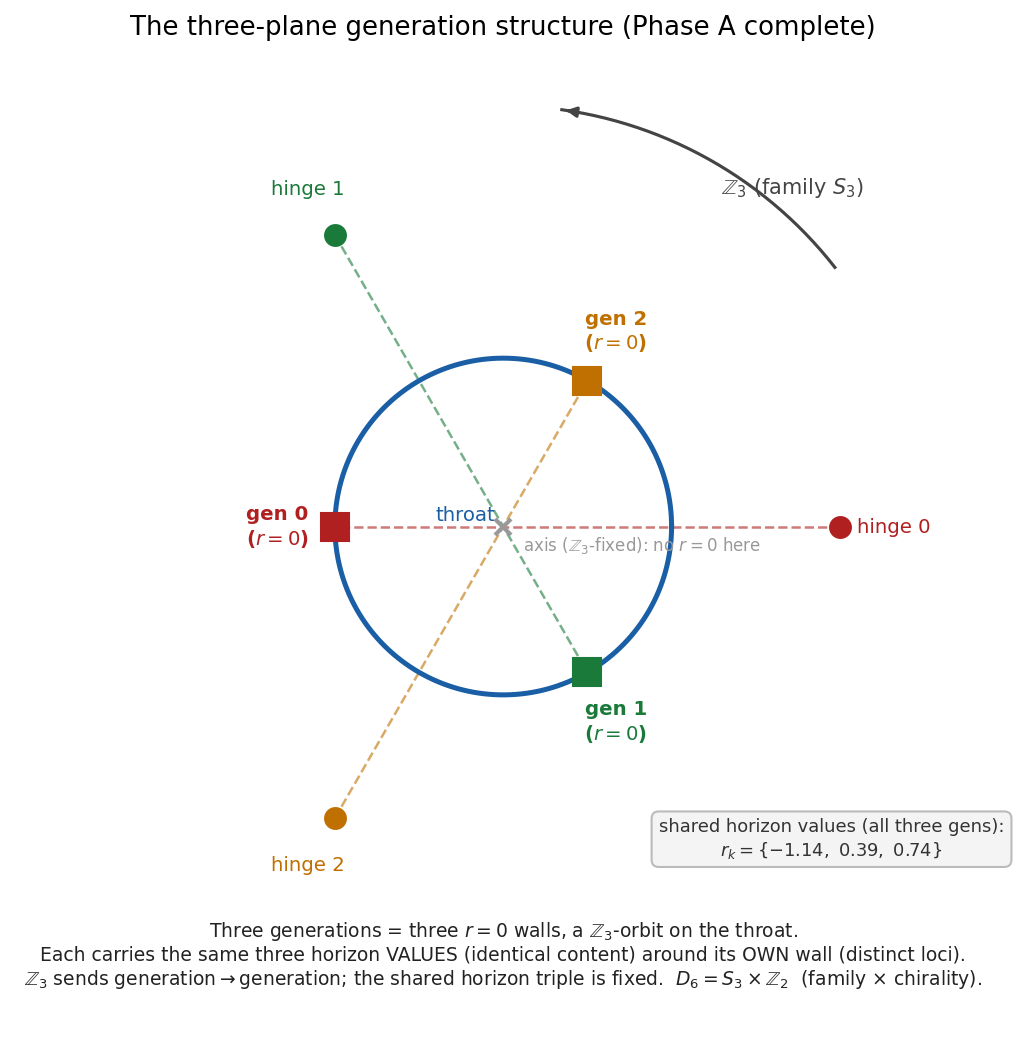
\includegraphics[width=0.62\textwidth]{figures/CR_three_generation_structure.png}
\caption{The three-plane fermion structure. Three hinges (radius $2\alpha$, polar $0/120/240$) and their three $r=0$ walls (on the throat circle, polar $180/300/60$, each antipodal to its hinge)---a $\mathbb{Z}_3$-orbit. Each plane carries the same three horizon \emph{values} (identical content) around its own wall (distinct loci): three identical generations. The centre (the $\mathbb{Z}_3$-fixed axis) carries no wall. $\mathbb{Z}_3$ sends generation to generation; $D_6=S_3\times\mathbb{Z}_2$.}
\label{fig:gen}
\end{figure}

Two constructions are geometrically available: one plane on one chosen hinge, or one plane on each. They are not on equal footing.
\begin{proposition}\label{prop:forced}
Within CR the three-plane construction is forced.
\end{proposition}
\begin{proof}[Argument]
A one-plane construction must select \emph{which} hinge to build on: a free modulus, unfixed by the geometry, an arbitrary choice among three $\mathbb{Z}_3$-equivalent options. The $\mathbb{Z}_3$-symmetric three-plane construction is the unique configuration carrying no such modulus---the symmetric point, pinned by the symmetry. CR is defined by maximal symmetry read as least-arbitrariness: the substrate is $\dS_5$ precisely because a less symmetric choice would be unforced~\cite{JanzenGeometricCore,JanzenCRframework}, and the geometric-core paper extends this to the discrete sector explicitly, holding that the discrete breaking is itself maximally symmetric. A construction carrying an unfixed arbitrary modulus is exactly what that principle excludes. The one-plane truncation is therefore not admissible within CR, and the three-plane structure is selected.
\end{proof}
The qualification is genuine and we state it plainly: Proposition~\ref{prop:forced} forces the count \emph{within CR}, resting on (i) the maximal-symmetry principle, which is the programme's definition rather than an added hypothesis, and (ii) that the fermion generations are set by the matter construction at all---Proposition~\ref{prop:wall} makes this concrete, but the link is itself the claim the sector establishes. It is not a free-standing theorem. Inside CR it is forced. Two remarks sharpen this. The two legs are in fact one: given the three-hinge leaf, the three throat walls are \emph{distinct} loci, so the wall-bound zero-modes have disjoint support and span a three-dimensional space---a flavour triplet, three physical states in any basis, not one state redescribed---so leg~(ii) follows from leg~(i) rather than standing beside it. And the pillar that remains, leg~(i), is the programme's own \emph{criterion of necessity}---Rule~2 of~\cite{JanzenShadowExistence} in the ontological register---for which a symmetry-breaking modulus (which of three $\mathbb{Z}_3$-equivalent hinges) is exactly the adjustable parameter it rejects, and maximal symmetry the structure that requires its configuration. ``Forced within CR'' is thus forced by that vindicated criterion, not an added axiom; the honest edge is that a framework declining the criterion reads the natural single-hinge index---one---not three. The direction of that dependence is worth stating, since \cite{JanzenShadowExistence} in turn cites this sector: the epistemic paper \emph{establishes} Rule~2 from the historiographic record, independently of any result here, and cites the three-plane selection only as a worked instance of the rule in the ontological register. The dependence is one-way and the mutual citation is not circular---this paper applies a criterion the other grounds elsewhere.

By Proposition~\ref{prop:wall} each of the three walls binds one chiral zero-mode; the three are localized at distinct walls, hence linearly independent. The generation count is the number of such modes, a wall-localized index insensitive to the non-compactness of $\dS_5$ that obstructs a bulk index~\cite{JanzenBoundary}: the modes are normalizable (in the leaf norm of Section~\ref{sec:chirality}) and pinned to the throat, and there are three. That count is a well-defined index in the precise sense CR's ontology makes available. In the leaf's proper measure $d\ell=dr/\sqrt{|f|}$ the closed slicing has \emph{finite} total length\rcpt{P14_leaf_compactness}---the horizon turning points at finite proper distance, the $r=0$ crossing an integrable $\sqrt{\,}$-singularity---so the leaf is compact and the Dirac operator on it carries a \emph{finite} analytical index $\dim\ker$~\cite{AtiyahSinger1968}, exactly where the bulk index on the non-compact spacetime (tortoise measure) is obstructed. \emph{The leaf is closed as well as compact}, and that is a second thing the measure delivers: with no boundary there is no Atiyah--Patodi--Singer correction and no $\eta$-invariant term, so the index is the interior one entire and the count is the whole of what the theorem returns.\ldg{spectral_theory} \emph{Compactness delivers finiteness and not canonicity, and the distinction is load-bearing here.} In the proper radial coordinate of the leaf frame, $\dd x=\dd r/\sqrt f$, the first-order
pair integrates in closed form: $\int W\,\dd x=\int(\lambda\sqrt f/r)(\dd r/\sqrt f)=\lambda\ln\lvert r\rvert$,
so the zero mode is a power law $\psi=\lvert r\rvert^{\pm\lambda}$ rather than the $\tanh$ model's exponential.
Near the branch point $f\to-2M/r$, so the leaf measure behaves as
$\dd\ell=\dd r/\sqrt{\lvert f\rvert}\sim\sqrt{\lvert r\rvert/2M}\,\dd r$ and normalizability of
$\lvert r\rvert^{s}$ requires $s>-\tfrac34$. The decaying branch $s=+\lambda$ satisfies this for every
$\lambda$; the growing branch $s=-\lambda$ would require $\lambda<\tfrac34$, which no $\lambda=j+\tfrac12$
attains. At the horizons the measure carries an integrable inverse square root and $\psi$ is finite, so the\rcpt{B67_verdict_the_analytic_sqrt_f_operator}. \emph{One numerical coincidence is worth disowning before anyone builds on it}: the threshold here is $\tfrac34$, and so is the essential-self-adjointness threshold the companion canonical paper meets at $a=0$~\cite{JanzenCanonicalTime}---but they are different computations. That one comes from $\sqrt{\gamma+\tfrac14}=1$ on exponents $\tfrac12\pm\nu$ in $\dd x$, an exponent gap of two; this one from $-2|\lambda|+\tfrac12=-1$ on a density in $\dd\ell$, a gap of three. \emph{Different measures, different gaps, the same number by arithmetic and not by structure.} \emph{Nothing in the count depends on a boundary condition}, the three modes having disjoint support and definite chirality either way. Each wall's mode is a definite chirality eigenstate $\sigma_y=+1=R=\gamma^5$ (Prop.~\ref{prop:wall}, the conjugate branch rejected), and the signed-radius flip is through the $r=0$ \emph{branch point}\rcpt{P14_mode_monodromy_at_the_wall} rather than a single-valued crossing on a loop~\cite{JanzenSlicing,JanzenCircle}---so the even-crossing constraint that binds a single-valued sign function on a circle does not apply, and the three same-chirality modes on disjoint support have no cancelling partner. Hence $\dim\ker_+=3$, $\dim\ker_-=0$, and the count is the net chirality: a $\gamma^5$-graded index. Index-theoretic stability under deformations preserving the three-wall structure is the expected behaviour of such a graded count and is traced rather than computed here (\rcpt{P14_even_crossing_index} establishes the mechanism---one mode per wall, the even-crossing obstruction on a simple loop, and the necessity of the $r=0$ branch point---and marks the Atiyah--Singer statement on the branched bead as traced); we state it at that weight\ldg{index_theory}. \emph{And it is worth saying which half is traced, because the two halves are not equally owed}: the \emph{analytical} index is $\dim\ker_+-\dim\ker_-$ by definition, so the count above is computed and needs no theorem; what the index theorem supplies is its equality with a topological integral, and what that equality buys is exactly the deformation invariance traced here. \emph{So the citation is honest rather than load-bearing for the count}, and the corpus's naming follows the same division---\emph{analytical index} appears and \emph{topological index} never does\rcpt{D1_the_traced_half_is_the_theorem_and_the_computed_half_is_not}. It is a leaf (vantage) index, which is why it is well-defined precisely where the spacetime bulk index is not.
\begin{equation}
\boxed{\ \text{number of chiral generations} \;=\; 3.\ }
\end{equation}

\paragraph{What the count fixes about the dimension.} The count above is read off the horizon
cubic through the three hinges, and that cubic is an output of the four-dimensional metric function
rather than an assumption of this sector. The constraint therefore runs the other way from the way
it is usually posed: \emph{the flavour content constrains the dimension}, rather than being handed
one.

In $D$-dimensional Schwarzschild--de~Sitter the mass is the slicing-dependent factor $2M=r_{0}^{D-3}-r_{0}^{D-1}$ in the gauge $\alpha=1$, and two conditions this construction already imposes then bear on $D$. The first is the collapse. The family is parametrised by the sky angle, and the horizon relation is required to linearise there to a \emph{single} multiple-angle---in the companion paper's words, the slicing scale $2/\sqrt3$ is ``the one scale removing the residual harmonic''~\cite{JanzenSlicing}. 

The two powers present are $D-3$ and $D-1$, so the harmonics standing below the top one number exactly \emph{one} at $D=4$ and $D=5$ and \emph{two or more} from $D=6$ upward, while the construction has one scale to spend: from six dimensions up no slicing scale collapses the relation, there is no forced fold, and the family carries no generation count to read at all. 

At $D=5$ the collapse does occur, at scale $1$, and returns a four-fold. 

The second condition is the parity, and it separates those two. The mass function is odd in the signed offset exactly when $D$ is even, so at $D=5$ the orientation parity $r_{0}\mapsto-r_{0}$ \emph{fixes} each geometry rather than exchanging it with its conjugate: there is no mass-reflection $\mathbb{Z}_{2}$, hence no $\mathbf 3\oplus\bar{\mathbf 3}$ Nariai hexad, no outer factor of $\mathrm{Aut}(A_{2})=S_{3}\times\mathbb{Z}_{2}$, and no $\gamma^{5}$---which is that parity's Clifford generator on the cut (Section~\ref{sec:twofactors}), and on which this paper's chirality rests through a superpotential odd in the signed radius (Section~\ref{sec:chirality}). A five-dimensional spacetime would therefore carry four generations and no handedness---and, \emph{on the same computation, no antimatter either}, since the parity whose absence removes $\gamma^{5}$ is the one whose absence removes the antifundamental.\rcpt{P14_the_d5_world} \emph{The two deliverables are one fact seen twice, and it is visible in the collapse itself}: at $D=4$ the relation collapses to a pure multiple angle $2M=\tfrac{2}{3\sqrt3}\sin 3w$ of zero mean, whereas at $D=5$ it collapses to $2M=\tfrac18(1-\cos 4w)$---one harmonic \emph{plus a constant}. 

Both are single-harmonic in the sense the collapse condition asks for, but the constant is not nothing: it holds $2M\ge0$ across the whole swing, so the mass never changes sign, and the sign change is the entire content of the mass reflection. \emph{And the same obstruction is visible a third time, in the root set itself, where it exhibits its mechanism.}\rcpt{P14_odd_D_contains_its_own_image} 

Writing the horizon condition with the slicing's own root substituted, $P_{D}(r)=r^{D-1}-r^{D-3}+r_{0}^{D-3}-r_{0}^{D-1}$, the factor $(r-r_{0})$ divides at every $D$---that is the designation split---and $-r_{0}$ is a root \emph{exactly at odd} $D$, since substituting it returns $2\cdot 2M$ at even $D$ and $0$ at odd. 

So at $D=5$ the cofactor degenerates to $(r+r_{0})(r^{2}+r_{0}^{2}-1)$, a line and a circle, and the $1+3$ is really $1+1+2$ with the extra one being $-r_{0}$ itself, where at $D=4$ the cofactor is a genuine conic and at $D=6$ and $D=8$ it does not factor at all. The root-set condition and the mass-parity condition are exact complements dimension by dimension, and the reason is structural: at even $D$ the reflection $r_{0}\mapsto-r_{0}$ carries the geometry to a \emph{different} member of the family, which is what lets it serve as a matter/antimatter parity, while at odd $D$ the reflected root already lies in the same geometry's own root set, so the parity has nothing to relate. \emph{The geometry is its own image, and that is why five is vector-like.} \emph{And two further structures fail at odd $D$ for the same evenness, the three being one fact.}\rcpt{P14_odd_D_is_pair_symmetric} 

The polynomial $r^{D-1}-r^{D-3}+2M$ has its two powers of one parity, so it is even in $r$ exactly at odd $D$; its root set is then stable under a fixed-point-free involution, and the monodromy over the mass plane commutes with that involution. 

At $D=5$ this confines the monodromy to the centraliser of $(0\,1)(2\,3)$ in $S_{4}$, of order eight against twenty-four, so the
monodromy group cannot be the full symmetric group on the roots and the four-dimensional statement that it is has no odd-dimensional analogue. 

The root set is likewise not of $A_{2}$ type: the roots sum to zero at every $D$, but at four that is three roots summing to zero, and at five it is four summing to zero \emph{in $\pm$ pairs}---so at five there is no $A_{2}$ whose automorphism group could factorise or fail to. \emph{The constant and the evenness are the same obstruction read in two variables}---and with no sign change there is no antifundamental, hence no hexad, hence none of the twelve designations the four-dimensional dial carries. Among the dimensions in which the count exists at all, four is the only one that also carries a chirality, so the two halves of this sector's own delivery---the number and the handedness---are jointly available at exactly one dimension\rcpt{P14_dimension_from_flavour}. Both conditions are read through the sky angle and so through the gnomonic chart, and that chart is not a four-dimensional import: the companion paper forces it by the straight-line criterion alone---a faithful planar chart must carry the straight line of sight to a straight line, and the gnomonic projection is the unique projection sending every great circle to one---``independently of the observer or the slicing scale''~\cite{JanzenSlicing}, a property of $S^{n}$ in every $n$, and the observer's celestial sphere in $D$ dimensions is $S^{D-2}$. (That paper's \emph{secondary} exclusion of the orthographic, which turns on $\sin\theta\le1<2/\sqrt3$, is specific to the four-dimensional scale and is not used here.) The altitude is the same as the rest of this section, and the one assumption is named: the $D$-dimensional metric function is taken to be the standard Tangherlini--de~Sitter one, an extension of the codimension-one operator rather than a rederivation of it at general $D$. Within CR, and at that weight, the observed flavour skeleton is not merely consistent with four dimensions but selects them.

\subsection{The correspondence, stated in Standard Model terms}\label{sec:correspondence}

Because the papers above speak of ``generations'' without saying what a generation contains, we set the
correspondence out explicitly. A reader who knows the Standard Model should be able to see at once which of its
structures this sector fixes and which it does not.

\emph{What a Standard Model generation contains.} In left-handed Weyl form, one generation is five irreducible
multiplets of $\su(3)_c\times\su(2)_L\times\mathrm{u}(1)_Y$:
\[
Q=(u,d)_L:(\mathbf{3},\mathbf{2})_{+1/6},\quad
u^{c}:(\bar{\mathbf{3}},\mathbf{1})_{-2/3},\quad
d^{c}:(\bar{\mathbf{3}},\mathbf{1})_{+1/3},\quad
L=(\nu,e)_L:(\mathbf{1},\mathbf{2})_{-1/2},\quad
e^{c}:(\mathbf{1},\mathbf{1})_{+1},
\]
totalling $6+3+3+2+1=15$ Weyl fermions, or $16$ with a right-handed neutrino
$\nu^{c}:(\mathbf{1},\mathbf{1})_{0}$\rcpt{P14_the_count_specified}. The quark/lepton distinction is exactly the first entry of each triple:
a quark carries the colour $\mathbf{3}$, a lepton the singlet $\mathbf{1}$. Three generations is $45$ (or $48$)
Weyl fermions in all.

\emph{What this sector fixes.} Three features of that skeleton, and only three.
\begin{itemize}
\item \emph{The number of generations is three}, as a $\gamma^5$-graded index of wall-localized zero-modes
($\dim\ker_+=3$, $\dim\ker_-=0$; Section~\ref{sec:count}).
\item \emph{Each is chiral}, carrying a definite $\gamma^5$ eigenvalue (Proposition~\ref{prop:wall}). This is
not decoration: the Standard Model's content is chiral, and a construction returning a vector-like spectrum
would be excluded by that fact alone.
\item \emph{The three are related by a global $S_3$} (Section~\ref{sec:family})---a family symmetry, not a
gauge symmetry.
\end{itemize}

\emph{What it does not fix, and the list is longer.} The internal content of a generation is untouched: how
many Weyl fermions it holds ($15$ or $16$), their $\su(3)_c$ representations---hence \emph{which of them are quarks and which are leptons}\rcpt{P14_quark_lepton_frontier}---and their $\su(2)_L$ doublet/singlet structure. \emph{The hypercharges are not a third undelivered item}: given those two, they follow from the per-wall anomaly conditions of \S\ref{sec:inflow} together with the existence of the Yukawa couplings, uniquely up to normalisation. Anomaly
cancellation, which the Standard Model's fifteen satisfy non-trivially and which is among the sharpest
constraints on any proposed content, is not addressed. Neither is the mass spectrum, the mixing, nor the
existence of $\nu^{c}$. \emph{The zero-mode of Proposition~\ref{prop:wall} is one Weyl mode per wall, not
fifteen}: the index counts generations, not the states within them.

\emph{Two consequences of stating it this way are worth drawing.} First, the correspondence is
$3\leftrightarrow3$ at the level of \emph{families}, with every representation-theoretic fact about the
Standard Model on the far side of the wall of~\cite{JanzenBoundary}; the sector is compatible with the Standard
Model's content in the weak sense of not contradicting it, and does not predict it. Second, the global $S_3$ is
a point of contact rather than a free addition: the Standard Model has no exact family symmetry---the Yukawa
couplings break it badly---so an exact $S_3$ delivered here must be broken by whatever supplies the masses, and
the manner of that breaking is a constraint this sector inherits rather than a freedom. \emph{We record that as
an obligation, not a result.} \emph{That obligation can be checked against a literature rather than left standing, and it is worth doing
because the check could have gone badly.} $S_3$ is among the most studied discrete flavour symmetries: the
$S_{3L}\times S_{3R}$ proposal predicting quark-sector flavour democracy has been followed by an extensive
body of work on how to break that democracy and recover realistic spectra and
mixing~\cite{HarariHautWeyers1978,XingYangZhou2010}. The structure of the symmetric limit is definite and
matches what a three-object permutation representation gives: the mass matrices take a universal two-term form,
one piece proportional to the identity and one to the democracy matrix. On that decomposition the observed
pattern is not accidental---the charged-fermion matrices are strongly hierarchical, the quark mixing matrix is
close to the identity, and the lepton mixing matrix carries two large angles, all as consequences of which term
dominates where~\cite{XingYangZhou2010}.

\emph{Two things follow for this sector, and they pull in opposite directions.} The obligation is met in the
sense that matters: an exact $S_3$ broken by the mass mechanism is a viable and worked framework, not an
excluded one, so the sector is not committed to a symmetry the data refute. But it is not met for free.
Realistic fits generally augment the group---$S_3\times Z_3\times Z_6$ in one construction, where the neutrino
sector's breaking supplies a naturally small solar-to-atmospheric ratio and next-to-leading corrections bring
$\theta_{13}$ into the measured range while the quark sector accommodates the Cabibbo angle and the differing
up- and down-type hierarchies~\cite{Meloni2012}---and the breaking pattern does substantial work. \emph{What
this sector supplies is the symmetry, not the breaking}: the $S_3$ arrives here from the substrate's geometry
rather than being posited, which is a point of contact worth having, while the breaking that generates the
observed masses and mixings remains external to it, in the same place as the gauge representations.
 The mass spectrum and the gauge representations are external to it and are so marked. This is the innermost of the three registers of maximal symmetry the geometric-core paper draws together~\cite{JanzenGeometricCore}: the substrate maximally symmetric, the evolving space maximally symmetric, and now the discrete matter structure maximally symmetric and counted.



\section{The family symmetry}\label{sec:family}

The three walls are permuted by the symmetry of the hinge triangle. The $\mathbb{Z}_3$ rotation cycles them ($180\!\to\!300\!\to\!60$); each of the three reflections---across the axis through one wall---swaps the other two and fixes it. The three transpositions and the three-cycle generate the full $S_3$. With the chirality $\mathbb{Z}_2$ of Proposition~\ref{prop:wall}, the discrete group carried by the sector is
\begin{equation}
D_6 = S_3 \times \mathbb{Z}_2 \qquad (\text{family}\times\text{chirality}),
\end{equation}
the automorphism group $\mathrm{Aut}(A_2)$ already identified as the substrate's discrete structure~\cite{JanzenSlicing,JanzenGroupoid,JanzenAlgebroid}.

\emph{Writing it as a product invites a question the product hides: $D_6$ has \textbf{three} subgroups of order six, and which one the sector carries is a physical statement rather than a labelling.} Exactly one is cyclic, $\langle\text{the Weyl }3\text{-cycle}\rangle\times\langle\gamma^5\rangle$---\emph{and it is worth saying that this is \textbf{not} the family symmetry paired with chirality}, since the $\mathbb{Z}_3$ inside $\mathrm{Aut}(A_2)$ rotates the three horizon \emph{roots} and is therefore the within-state index of \S\ref{sec:whichthree}, while the generations' own $\mathbb{Z}_3$ is the turnaround's deck, which fixes the horizon cover's base and never permutes its fibre and so is no subgroup of this group at all---and the other two are \emph{both} isomorphic to $S_3$ while being different subgroups: $S_3\times1$, in which the roots are permuted and the chirality untouched, and the graph $\{(\sigma,\operatorname{sgn}\sigma)\}$, in which every root transposition carries a chirality flip. \emph{The boundary paper's own reading of the hexad settles which}: there $\sigma$ exchanges a pair \emph{within} a sign-half while the backward-radial reflection---the outer $\mathbb{Z}_2$---is what carries between the halves~\cite{JanzenBoundary}, so a transposition carries trivial $\mathbb{Z}_2$ component and the family symmetry is $S_3\times1$ and not the twisted graph. \emph{Root transpositions do not flip chirality}, which is why the three walls can be same-chirality at all (\S\ref{sec:count}).

\emph{Two further facts about this group are established elsewhere and bear directly on the sector.}

\emph{First, the group is larger than $D_{6}$, and the excess is substrate-derived.} The residue pairing that
the horizon roots' surface gravities put on the root triple has a holonomy about the Nariai points---the Klein
four-group of even sign changes, arising as the per-root resolution of $\sqrt{\Delta}$, the same square root
whose non-squareness fixes the Galois group as $S_{3}$~\cite{JanzenGroupoid}. Adjoined to the walls' $S_{3}$ it
closes $W(A_{3})$ in its Weyl embedding, and with the chirality parity a group of order forty-eight; and
$A_{3}$ is the root system of $\so(6,\mathbb{C})$, the complexification of the substrate's own isometry
algebra, with $A_{2}$ inside it by deleting one node~\cite{JanzenAlgebroid}. \emph{So the sector's discrete
group is the substrate's own, where this section has been reading a sub-root-system of it.}

\emph{Second, and physically, that holonomy acts on the walls' chiralities and protects the count's parity.} By
Proposition~\ref{prop:wall} each wall's chirality is a definite $\sigma_{y}$ eigenvalue whose sign is the sign
of the signed-radius flip, so a sign change is a reversal of that wall's chirality; the holonomy's elements
change signs in \emph{pairs}, unimodularity excluding every odd change. \emph{The observed configuration is
accordingly the unique member of its orbit with all three walls at one chirality}, and $\dim\ker_{-}$ cannot be
reached from $\dim\ker_{+}=3$ by any number of loops, three and zero lying in different parity
classes\rcpt{V4_chirality_parity}. \emph{The count is thus not merely what the index returns but what no
holonomy of this connection can move.} \emph{Two guarantees are in play here and are worth keeping apart}: compactness of the leaf makes the
count \emph{defined}, and what makes it \emph{stable} is the wall's spectral gap---its bound modes are
separated from the continuum by the full asymptotic mass, so no small deformation of the wall carries a
state across the threshold and changes the number.\ldg{spectral_theory} 

That the family symmetry the three walls carry is \emph{global} rather than gauged is not a choice made here but the \emph{kind} the discrete structure fixes: the Weyl $S_3$ is the
monodromy symmetry of the solution space and no substrate isometry, whereas the orientation parity $\mathbb{Z}_2$ \emph{is} an isometry, acting on the cut spinor as $\gamma^5$---so chirality descends gauged and flavour global, the Standard Model's own arrangement following from which factor is an isometry~\cite{JanzenGroupoid,JanzenAlgebroid}. 

That chirality rides the \emph{discrete} factor is moreover forced, not merely sorted: a chirality carried by a connected-group isometry would be rendered vector-like by the Atiyah--Hirzebruch index obstruction, so an observed chirality can live only on the discrete orientation parity that obstruction cannot reach~\cite{JanzenBoundary}. 

Each plane carries the same three horizon values, so the three generations are identical in content, distinguished only by their wall; this is why the family symmetry is a symmetry of \emph{identical} copies, the defining property of Standard-Model generations. And the wall is not a bare locus. Each hinge \emph{designates} one of those three roots as its own black-hole horizon, so a transposition of roots is a hop to a neighbouring hinge, and the Weyl $S_3$ \emph{is} the relation among the three hinges rather than an abstract relabelling~\cite{JanzenSlicing}. The $S_3$ the three walls carry and the Weyl $S_3$ of the root system are therefore \emph{one group}, not two that happen to agree in order: a generation is the vantage that takes its own root as its hole, and which root it takes is the same distinction as which wall it binds at---the hinge fixes both. This is what makes ``one object read three ways'' a statement about the sector rather than about the cubic alone: the three readings are the three hinges, and the fermion sector is where they become three states. At the massless level the three are degenerate and $S_3$ is exact, and this degeneracy is \emph{forced}: the three shared horizons are roots of one cubic $r^3-r+2M=0$, and every root, designated the slicing parameter, returns the \emph{same} $2M=r_0-r_0^3$ (as $r^3=r-2M$ for each), so the three carry one mass parameter---one object read three ways on the fully $D_6$-symmetric horizon locus, a diagonal line and a $45^\circ$ tilted ellipse in the $(r_0,r)$-plane~\cite{JanzenSlicing}, on which the $2{+}1$ of a designated root against the ellipse pair is the diagonal designation $\sigma$ and the sign $2{+}1$ (two horizons of one sign against one) the reflection through the origin ($2M\mapsto-2M$, the chirality parity), each a description structure paired with its symmetric twin---so no asymmetric handle sits in the mass \emph{parameter}. The locus does carry a flavour-\emph{breaking structure} (the slicing singles one root against the ellipse pair), supplied with the triplet in the boundary paper~\cite{JanzenBoundary}; but the mass \emph{values} are the ordinary electroweak route, and whether that geometric structure is the physical hierarchy is not claimed---outside the present scope.

\section{The two factors: why they differ in kind}\label{sec:twofactors}\ldg{combinatorics}

The sector's two data are a chirality and a count, and Section~\ref{sec:family} has just written them as the two factors of one group, $D_6=S_3\times\mathbb{Z}_2$ (family $\times$ chirality). Two things about that group have been established elsewhere and are used above: that its factors act on independent structures---the Weyl $S_3$ on the three horizon roots and the inversion on the two null rulings, the inversion central~\cite{JanzenAlgebroid}---and that they descend differently, one gauged and one global. \emph{The product's being direct is worth separating from both, because it is forced and therefore carries no information about this substrate}: $\mathrm{Aut}(A_2)$ is a Weyl $S_3$ extended by a diagram $\mathbb{Z}_2$, every automorphism of $S_3$ is inner, and a semidirect product by an inner automorphism is isomorphic to the direct one---so there was never a semidirect alternative for the geometry to have excluded. 

What the geometry supplies is which relation each factor bears to the substrate's waist, and that the two differ in kind; the group structure follows and does not evidence it. 

Both have been read off the constraint algebra and off the light cone~\cite{JanzenAlgebroid}. \emph{And the chirality factor has a second realisation, in a sector with no fermions in it, which is worth
stating because it shows the parity is the substrate's and not this sector's.} In the radiating sector the same
$\mathbb{Z}_2$ appears as the graviton's two helicities: chirality there is the turning of the polarization
plane, the sign of the rate at which the polarization angle turns, \emph{absent} wherever a residual connected
isometry pins the polarization to a fixed axis---the swept $\mathrm{SO}(3)$ of the symmetric sector completing a
reflection into a rotation and identifying the two handednesses, a mirror and not a chirality---and genuine
once that swept rotation is lost~\cite{JanzenDynamics}. \emph{That is the same mechanism operating here, by a
different instrument.} 

What makes the wall's bound mode chiral rather than mirror-paired is that no connected
group identifies its two handednesses, which is what the index obstruction of~\cite{JanzenBoundary} says of a
connected gauge action and what confines the parity to the disconnected component. \emph{In the radiating
sector the identification is lifted by losing a residual isometry and the matter is a direct computation; here
it is barred by a theorem about connected groups}---one parity, two sectors, two instruments. The
corroboration runs the way that matters: a sector with no fermion content returns the same $\mathbb{Z}_2$, so
the factor read off the light cone is a feature of the substrate rather than an artefact of the wall
construction. A third route reaches the same factorisation from the numerals alone, and reaches it without being told to look: an audit of the recurring numbers of the construction, asking of each pair only whether one object derives both, returns every weld through one of these two factors---the triple-angle map for the three, the twelve, the thirty, the $\sqrt3$ and the $\sqrt[3]{2}$; the ruling-exchange for the two---and every proved split across them, so that the numbers weld \emph{within} a factor and split \emph{across} it. 

The audit, its receipts, and the splits that cut its law are collected in the programme's combinatorics ledger (\texttt{COMBINATORICS\_LEDGER.md}; \rcpt{P14_L8_the_three}, \rcpt{P14_L8_the_two}, \rcpt{P14_L8_the_twelve}), alongside the figure programme's. Read on the substrate's waist they are one fact, and this is the paper to state it in, because this is where the two factors become matter: the $\mathbb{Z}_2$ as a bound state's chirality eigenvalue (Proposition~\ref{prop:wall}), the $S_3$ as a count of three (Section~\ref{sec:count}). Because that $\mathbb{Z}_2$ is a substrate isometry it grades a chirality in the radiative sector as well as this one---the graviton's two helicities~\cite{JanzenDynamics} and the fermion's $\gamma^5$ here are the one gauged factor's two physical faces, the same $\mathbb{Z}_2$ read in the two sectors, settled there by direct computation on the free wave and here by the domain-wall zero-mode. Its radiative face becomes a \emph{genuine} chirality only past the wall of the symmetry-reducible sector, where the last swept $\mathrm{SO}(3)$ is lost and no isometry survives to turn the exchanging reflection into a rotation---the geometric onset of the parity the fermion sector here carries as $\gamma^5$~\cite{JanzenRange}.

The two structures the factors act on are the two relations a figure can bear to a circle. The three roots are the three special points \emph{on} the throat circle: an offset line meets it at two points $A$ and $B$, with $r=0$ fixed at the back, and those three points are the geometric counterparts of the three roots of the horizon cubic~\cite{JanzenSlicing}---which is why the walls of Section~\ref{sec:count} lie on that circle and not elsewhere. That offset \emph{is} the mass---matter as the bend of the cut, $G$ entering only as the offset-length---so the same offset furnishes both factors geometrically: its odd offset--mass relation ($2M\mapsto-2M$) is the chirality parity, and its three roots the count~\cite{JanzenOperator}. The two rulings are the lines \emph{tangent} to it: the substrate's null rulings \emph{are} the tangents to its waist, ``doubly ruled by straight null lines'' and ``every tangent to the throat is null'' being one statement, the power of a point with respect to that circle being the square of its height~\cite{JanzenGeometricCore}. So the automorphism group factorises because \emph{on} and \emph{tangent} are independent relations to one circle; the direct product is that independence. That there is a second factor at all is itself contingent: the inversion is an \emph{outer} automorphism---not already inside the Weyl $S_3$---only because the cubic realises $A_2$, the one rank-two system with $-1\notin W$; were negation inner (as for $A_1$, $B_2$, $G_2$) $\mathrm{Aut}(A_2)$ would collapse to the Weyl group and leave no chirality factor to sort, which the groupoid paper marks the condition of there being two factors at all~\cite{JanzenGroupoid}. The on/tangent independence is then why the two that do exist form a \emph{direct} product.

And the factors differ in \emph{kind} for the same reason, which is why the difference is not an extra fact requiring its own argument. A tangent is a line \emph{of} the substrate, so exchanging the two rulings is a motion of the substrate---an isometry, acting on the cut spinor as $\gamma^5$, and the chirality descends \emph{gauged}. A root \emph{labels a different cut}, so permuting the three moves through the solution space and is no motion of the substrate---the
monodromy symmetry, and the family symmetry is \emph{global}. The same distinction is what the algebroid paper reads off the light cone, in the same objects: the sky-angle periodicity is two steps along a null ruling, hence a closed path of light and an isometry, whereas the Weyl reflection is a loop in the complex $2M$-plane, and $2M$ labels the family rather than pointing along the manifold~\cite{JanzenAlgebroid}. The two readings are one reading, because the ruling and the tangent are one line.

The Standard Model's arrangement of a gauged chirality against a global flavour is therefore, in this reading, the difference between being \emph{on} the one circle and being \emph{tangent} to it---and the present sector is where that difference becomes two physical data: a bound state's chirality eigenvalue, and a count of three. Two qualifications keep the statement at its weight. It explains the \emph{kind} of each factor and not the gauge content, which stays walled~\cite{JanzenBoundary}; and it is a reading of structure already established rather than a new derivation---what it adds is that the two structures, and hence the two kinds, are one circle's two relations, so that the arrangement follows from the geometry having a waist rather than from a further principle.

\section{The cosmogenesis of the generations}\label{sec:cosmogenesis}

The generations are wall-modes of the existent leaf (Section~\ref{sec:count}), and CR's cosmogenesis carries that leaf across the branch point at $r=0$, where collapse continues as cosmology~\cite{JanzenBoundary,JanzenCRframework}. Three features of the crossing fix what becomes of the generations, each read off established structure. \emph{Inheritance:} the causal reassignment fixes the expansion rate and does not touch the leaf-carried content, so the generation structure---being leaf-carried---is inherited across the branch point unchanged \emph{on the conjectured rate-only reassignment}, a placement the corpus has not derived, the fermion-sector reading of the corpus's rate-reassigned, matter-inherited law. 

This is the matter-sector face of the layered reading the cosmology computes on: the reassignment acts on the \emph{lapse}---the stacking rate, which it resets to the geometry-set law---and not on the \emph{leaf}, whose bend is the content~\cite{JanzenOperator,JanzenCRframework}; so the generations, being leaf-carried, cross as inherited content exactly as the radiation and matter densities do, the fermion instance of the general fact that at the seam only the rate is reset and everything the leaf carries passes through. \emph{A second argument reaches the same conclusion without the conjecture, and it is worth having because
it does not depend on what the reassignment touches.} The walls are not carried \emph{through} the crossing:
they are \emph{at} it. 

The signed areal radius passes through zero at a point on the throat circle, which is
why the walls lie on that circle and not elsewhere (\S\ref{sec:chirality}), so the wall locus and the branch
point are one locus. And the segment terminating there occupies no cosmic time at all---the real part of the
complex cosmic time does not advance along it, so the crossing is a boundary of zero duration rather than an
interval~\cite{JanzenCanonicalTime,JanzenCRframework}. \emph{A structure localized at a boundary of zero
duration has no interval in which to be altered}, whatever a reassignment acts on. The inheritance therefore
does not rest on the reassignment being rate-only: even one that touched the leaf would have no elapsed time in
which to touch it. \emph{What the rate-only placement adds, if it holds, is that nothing acts on the leaf at
all; what the zero-duration argument gives without it is that nothing could.} \emph{Origin:} the Nariai crest~\cite{Nariai1951} is the fixed point of the root-permutation, where two of the three roots merge (the discriminant $4-3r_0^2$ vanishing); the three generation-loci are $S_3$-symmetric there and split into three distinct generations undercritical, so the family structure \emph{originates} at the crest and unfolds as the universe expands. \emph{Chirality:} the crest is a fixed point of $S_3$ but \emph{not} of $R$~\cite{JanzenBoundary}, so the parity $R=\gamma^5$ is untouched---the inherited matter stays chiral, and no matter/antimatter asymmetry is a cosmogenesis event; it stays the ordinary route. 

This is rooted in the substrate's discrete geometry. 

The chirality/mass parity $R=\gamma^5$ is the mass-reflection $r_0\mapsto-r_0$ (equivalently $2M\mapsto-2M$), the orientation/diagram-automorphism parity, realised on the cut spinor as $\gamma^5$; as the $A_2$ diagram automorphism it carries the fundamental $\mathbf 3$ to the antifundamental $\bar{\mathbf 3}$~\cite{JanzenSlicing,JanzenAlgebroid}, and on the wall mode it is an exact operator (Proposition~\ref{prop:wall}). So the $R$-image of a generation is its antifundamental, and within CR that is its \emph{antimatter}: the dual $\bar{\mathbf 3}$ branch is antimatter at exactly the weight the fundamental branch is matter---forced within CR by the same discrete residue, with the world-correspondence of the identification the data's to judge as it is for the matter it pairs. 

The discrete matter/antimatter skeleton---representation ($\mathbf 3$ vs $\bar{\mathbf 3}$), chirality ($\gamma^5$), and mass-sign ($R$-odd $2M$)---is what the geometry supplies on both sides of the pair; the charge structure that closes $C$ is field-level on both sides equally, not a substrate datum---the charge entering the geometry only as the $R$-even $Q^2$, so charge conjugation is present there as a symmetry rather than an absence and is no substrate isometry, the outer $\mathbb{Z}_2$ of $\mathrm{Aut}(A_2)=D_6$ being $R$ and not $C$~\cite{JanzenBoundary}---so that geometry supplies matter's discrete skeleton and not its charge is no more an obstacle to naming the $\bar{\mathbf 3}$ branch antimatter than to naming the $\mathbf 3$ branch matter. 

What $R$ is \emph{not} is the time reflection $T$: they are distinct reflections---$R$ spacelike and horn-preserving, $T$ timelike and horn-flipping, so $R\neq T$ on the substrate's $A_2$ hexad, established in the slicing paper~\cite{JanzenSlicing}. 

That distinctness is exactly why the matter/antimatter parity is \emph{not} a cosmogenesis (time) event: antimatter is the substrate's ordinary $R$-partner of matter, not something made at the seam, which the crest, a fixed point of $S_3$ but not of $R$, leaves untouched. Read on the cosmogenesis, this same $R$-partner branch is not abstract: it is the conjugate ($r<0$) branch of the bead, the completed collapse whose future is our expansion, so the progenitor of our own universe sits on it---an antimatter black hole, in the signed-radius continuation~\cite{JanzenCRframework}. 

The relation is therefore standing and relational (our matter and the progenitor's, the two ends of one $R$-conjugation across the bead), consistent with its being no seam-generated asymmetry. $R$ is likewise distinct from the areal-radius spatial parity $r\mapsto-r$---the corpus's $P$---whose Clifford generator $\gamma^1\gamma^2\gamma^3$ anticommutes with $\gamma^5$.\footnote{Corpus convention: $R$ is the orientation/mass-reflection parity, the $A_2$ diagram automorphism $\in\mathrm{O}(5,1)\setminus\mathrm{SO}_0(5,1)$, realised on spinors as $\gamma^5$, carrying $\mathbf 3\leftrightarrow\bar{\mathbf 3}$; $P$ is the areal \emph{spatial} parity $r\mapsto-r$ ($\gamma^1\gamma^2\gamma^3$, anticommuting with $\gamma^5$); $T$ is the time reflection. The two parities are distinct, anticommuting operations, uniformly named this way across the corpus. \emph{And one further convention, fixed here because its absence has cost more than the parities' did}: \textbf{``the wall'' and ``the branch point'' denote the wall of the hinge under discussion.} There are three, one per hinge, at distinct points of the throat circle with disjoint support, and each vantage's signed areal radius vanishes at its own and at neither of the others~\cite{JanzenSlicing}. The bare singular is used throughout because the natural sentence is about one of them at a time; \emph{the test a reader should apply is that a sentence which would be false if there were three is a sentence about a single vantage and must name it}. This is stated because the sector's own winding computations had been read as though the wall were unique, which makes the branched cover cyclic and its monodromy abelian, and the whole of the colour structure is the difference between that reading and the correct one.\rcpt{P14_naming_a_derived_object}} The wall-mode's dynamics transitions with the reassignment: under the signature flip the hole-side spatial mass $W=\lambda\sqrt f/r$ passes into a cosmological-side temporal term (its turning imaginary past the horizons being precisely this), so the bound wall-mode continues as a fermion propagating in cosmic time, and the three progenitor wall-modes become the three propagating families of the expanding universe, carried through faithfully by the null characteristic seam. 

The explicit continuation of the exact zero-mode onto the cosmological leaf is carried out on a concrete undercritical model (receipt: \rcpt{P14_B2_zeromode_continuation}): the superpotential $W=\lambda\sqrt f/r$ is real between the horizons, where the mode is the exponentially bound wall-state, and turns imaginary past a horizon ($f<0$), where the same mode becomes a pure phase---a fermion propagating in the now-timelike radius; on the $E=1$ expanding leaf $r(\tilde\tau)\propto\sinh^{2/3}$ this is the standard massless-Dirac form of conformal weight $a^{-3/2}$, \emph{which is field-theory bookkeeping on a chosen chart and not a substrate structure}---the weight is the one a massless spinor carries on any Friedmann leaf, claimed here for the continuation and for nothing more\ldg{conformal_geometry}, so each of the three progenitor wall-modes continues term for term into a propagating family and the $\gamma^5$ chirality, untouched by the real-to-imaginary continuation, is preserved. 

Inheritance, origin, chirality, and the bound-to-propagating character stand on the crossing's established null-characteristic machinery. 

The universe those three families cross into is the one whose primordial light-element abundances the cosmogenesis paper computes~\cite{JanzenCosmogenesis}---the same branch-point crossing, read on the inherited radiation content rather than the fermion leaf, fixing the thermal history the abundances record. 

As throughout, this is coherence within CR; what the world's matter is remains the data's to judge.

This realises, on the built sector, the positive closure the boundary paper draws~\cite{JanzenBoundary}. There charge conjugation is shown to factorise on the cosmogenetic bead, $C=(Q\mapsto-Q)_{\mathrm{field}}\circ(R\circ K)_{\mathrm{geometric}}$, its kinematic (Feynman--St\"uckelberg) face carried geometrically by the composite of the mass-reflection $R$ and the cosmic-time reality involution $K:\tilde\tau\mapsto\bar{\tilde\tau}$, only the electric-charge sign closing from the field. On the present sector that geometric face acts on the \emph{actual} zero-modes: $R$ carries each matter generation's wall-mode to the bound opposite-chirality mode on the reversed ($r<0$, $2M<0$) wall---its antimatter partner $\bar{\mathbf 3}$, exact by Proposition~\ref{prop:wall}---and $K$ is the very real-to-imaginary seam continuation that carries the bound wall-mode to the propagating cosmic-time fermion above, so $R\circ K$ acts on the built modes as charge conjugation's kinematic face, the particle$\leftrightarrow$antiparticle relation of that conjugation being the two ends of this sector's $R$-conjugation across the bead (receipt \rcpt{P14_P14_payoff}). It is that face and no more, exactly as the boundary requires: the zero-modes carry the discrete flavour skeleton and not the gauge charge, so $R\circ K$ carries the discrete matter/antimatter conjugation while the electric-charge sign stays field-level---the identification of a mode with a \emph{specific} charged particle, and the full antilinear $C$, remaining the ordinary route. The operator half is explicit and grounded---the reality-involution lift $S=\gamma^{0}\gamma^{1}\gamma^{3}$ gives $\gamma^{5}S=-\mathrm{i}\gamma^{2}=-(C\gamma^{0\top})$, implementing $\psi\mapsto\psi^{c}$ on the cut spinor (\texttt{storyboard\_receipts/A3\_spinor\_lift.py})---but it is an operator identity carrying no charge, so the matter/antimatter \emph{pairing} of the two ends rests on the actual disjoint wall-modes of Proposition~\ref{prop:wall}, not on the operator alone; absent that built construction the frequency-wing/species identification would stay do-not-assert. The factorisation the boundary paper states is thereby realised on the sector it walls, at exactly its earned weight, and no further: coherence within CR, the world-correspondence the data's to judge.

\subsection{Which three the generations are seated on, and why it is not the hinges}\label{sec:whichthree}

The count above is read off the three walls and the family symmetry off the three hinges. \emph{Those are
one three, and it is not the generations' three}---which the substrate's null structure settles, from
outside this sector and by a fact the hinge reading cannot reach.

The substrate's null structure admits a \emph{bound} triple---a puncture of a hinge together with the two
punctures its null generators reach---and the causal classification of the six hinge-ends forces such a triple
to take one puncture per hinge: two ends of one hinge are timelike separated, two on one horn spacelike, and
only the cross pairs null.\rcpt{P03_hexagon_null_triple} A bound triple is therefore one-per-hinge without
choice. If the three hinges were the generations, a bound triple would be one constituent from each
generation, which is not what a bound triple of like constituents is. \emph{So the hinge three is the index
that distinguishes constituents within a bound state, not the index that distinguishes copies of the whole
state}, and the generations must be seated elsewhere.

They have somewhere to go, and it is the construction's own second three. The framework paper establishes that
no affine change of variable identifies the horizon roots with the roots of the comoving turnaround
(\emph{lem:twoturnings}); the marginally-bound congruence integrates to $r^{D-1}=2M\alpha^{2}\sinh^{2}\bigl((D-1)\tilde\tau/2\alpha\bigr)$
in $D$ dimensions, and the shift $\tilde\tau\mapsto\tilde\tau+2\pi i\alpha/(D-1)$ leaves $r^{D-1}$ invariant while
sending $r\mapsto e^{2\pi i/(D-1)}r$, so that second three carries a cyclic deck action of order
$D-1$.\rcpt{P03_the_weld_and_the_two_folds} Three consequences follow, and the third is the one that made the
move admissible.

\emph{First, the count is unchanged and the dimension argument with it.} Both threes are $D-1$, and for one
reason: clearing denominators, $f=0$ is a polynomial of degree $D-1$, and the two are the two things one does
with that single polynomial---the horizon three is its zero set, the turnaround three the deck action of the
integral of $1-f$. The fold is therefore a property of $f$ and not of which structure reads it, so
Section~\ref{sec:scope}'s conclusion---that four is the only dimension carrying both a count and a
handedness---holds on either seat, its $D=5$ member included.

\emph{Second, the family symmetry the generations bear is a different group from the hinges', and the
difference is substantive rather than a matter of naming.} The Weyl $S_{3}$ of Section~\ref{sec:family} is the relation among the three hinges, and on this
reading that is a statement about the within-state index: its transpositions are the hops between hinges that a
bound triple needs in order to be a singlet. The turnaround three carries the cyclic deck action alone. So the
family symmetry the generations bear is $\mathbb{Z}_{3}$, and $\mathbb{Z}_{3}<S_{3}$ properly.

\emph{Third---and this is what had to be checked before any of it could be said---the chirality survives.} The
grading is the mass reflection $R$, and $R$ acts on the turnaround branch: under $M\mapsto-M$ the right-hand
side of the law above becomes non-positive for real $\tilde\tau$, so a real image exists exactly when $D-1$ is
odd, and its image is $r\mapsto-r$, the signed radius. That condition is \emph{$D$ even}---the same condition
Section~\ref{sec:scope} already reads off $2M=r_{0}^{D-3}-r_{0}^{D-1}$ being odd in the signed
offset.\rcpt{P03_R_reaches_the_turnaround} The parity argument therefore transfers to the new seat without
modification. Composed with the deck action it gives $\mathbb{Z}_{6}=\mathbb{Z}_{3}\times\mathbb{Z}_{2}$.

\emph{That is not the whole of what the turnaround carries, and the correction is worth making here because it
runs the opposite way to what one would expect and does not disturb the argument
above.}\rcpt{P14_turnaround_carries_D6} It is natural to read the $\mathbb{Z}_{6}$ as an index-two subgroup of
the $D_{6}$ the hinges carry, with the missing part exactly the transpositions the within-state index needs.


\emph{The transpositions are not missing.} The time reflection acts on cosmic time as
$\tilde\tau\mapsto-\tilde\tau$, and the outward law $r^{3}=2M\alpha^{2}\sinh^{2}(3\tilde\tau/2\alpha)$ is exactly
invariant under it, $\sinh^{2}$ being even---so $T$ descends to the turnaround. But it does \emph{not} commute
with the deck action: it conjugates it to its inverse, $TDT^{-1}=D^{-1}$, which is the dihedral relation. Hence
$\langle D,T\rangle\cong S_{3}$ and, with the parity adjoined, the turnaround carries $D_{6}$ of order twelve
after all. \emph{What keeps this from collapsing the distinction drawn above is that the two $S_{3}$'s permute
different triples}---the hinge one the three horizon \emph{roots}, this one the three cube-root
\emph{sheets}---and the companion framework paper's \emph{lem:twoturnings} establishes that no affine change of
variable identifies the two root sets. \emph{The statement is available in the stronger form the seating here
actually wants}: the turnaround's deck carries a root of the horizon cubic to a root of the same cubic only at
$r=0$, since $(\omega r)^{3}-\omega r+2M=r(1-\omega)$ on the root variety, so it \emph{fixes} the horizon
cover's base and does not permute its fibre---and the two threes are therefore not related by any
covering-space construction, rather than merely by no affine
one\rcpt{P14_the_two_threes_are_not_related_as_covers}. \emph{Seating the generations on the turnaround rather
than the hinges needed the two threes to be genuinely different objects}, and had the turnaround deck been a
storey of the horizon cover's tower this subsection would have had no room to move. 

So the hinge transpositions remain the within-state index's; the
turnaround simply has transpositions of its own---\emph{though whose transpositions they are is worth saying,
because it decides what kind of family symmetry this sector delivers.}\rcpt{P14_the_family_symmetry_is_cyclic}


They are supplied by $T$, the horn swap, which this paper reads as weak isospin; so the turnaround's $S_3$ is
the family $\mathbb{Z}_3$ extended by an operation belonging to another sector, and reading it as a family
$S_3$ would be counting isospin as flavour. \emph{The family symmetry proper---the part acting on generations
and on nothing else---is cyclic.} A second consequence follows from the same computation and settles a
question this sector had been asking in a form that admitted no answer: since $T$ descends as the
\emph{inversion} $k\mapsto-k$ of the sheet index rather than as a translation, the change it induces is $0$,
$1$ or $2$ according to $k$, so ``the winding change under $T$'' is not a quantity at all. \emph{What is true
instead is sharper}: $T$ fixes the triality-neutral class and exchanges the two charged ones, which is the
action the orientation reflection already has,\rcpt{P14_the_lap_orientation_is_derived} and is consistent with
this paper placing conjugation at the branch point rather than on the horns. \emph{One consequence is worth recording without being
claimed}: the representations of $D_{6}$ that are trivial on the deck $\mathbb{Z}_{3}$---which is what carrying
no colour would mean---are its four one-dimensional ones, so a colourless sector on this structure has total
dimension four. 

\emph{That is a count of gradings and not of fields}, and this paper draws nothing from it. \emph{One thing should nevertheless be said about its shape, because the natural objection to it is misdirected.}\rcpt{P14_colour_is_vector_like_on_singlets} Every $\mathbb{Z}_2$ grading splits those four $2+2$, which looks like a failure to reproduce a colourless sector that is chirality-asymmetric. \emph{It is not a failure, because colour does not see the chirality of a colour singlet in the Standard Model either}: $SU(3)$ acts trivially on $\nu_L$, $e_L$, $e_R$ and $\nu_R$ alike, and what distinguishes the doublet from the singlet is $SU(2)_L$. A colour structure delivering a chirality-asymmetric colourless triple would not match the Standard Model but exceed it. \emph{The asymmetry is an isospin property, and the question properly addressed to this construction is whether $T$ acts on one $\gamma^{5}$-eigenspace of the wall mode and trivially on the other}---which is well-posed here, since $T$ and $R$ act on independent data and commute, so that $T$ acts within each chirality eigenspace separately. \emph{That they commute is the requirement rather than an obstruction}: a chiral action needs simultaneous diagonalisability, not its failure. \emph{One half of that question decides whether the other can be asked of this geometry at all, and it is settled}\rcpt{W1_the_two_plus_one_plus_one_is_excluded_by_a_symmetry_the_chiral_member_does_not_have}. 

Let $\sigma$ be the involution exchanging the two $\gamma^5$-eigenspaces---the reflection the companion paper's criterion calls the identifier of the helicities. 

It moves the ruling datum and not the horn datum, so it commutes with $T$ for the same independence that makes $[T,R]=0$; and then $T|_-=\sigma\,T|_+\,\sigma^{-1}$, so the two restrictions are conjugate and have the same orbit structure. \emph{Acting on one eigenspace and trivially on the other is precisely a difference of orbit structure, so it is excluded whenever $\sigma$ is a realised symmetry}---which, by that same criterion, is exactly the polarised case. 

Enumerating the four actions $T$ may take, the two with orbits $2+1+1$ are the two that admit no commuting $\sigma$, and the survivors are $2+2$ and $1+1+1+1$: the shape reported above is the only shape available. 

\emph{The statement is sharper as one about invariants}: on the achiral member every invariant is blind to the chirality, since $\sigma$ exchanges the eigenspaces; on the unpolarised member the conserved twist $c$ is odd under $\sigma$ and so separates them, and $c=0$ is the polarised cut---the two cases being one charge at two values. 

\emph{And the positive half is settled, in the negative}: the geometry \emph{permits} the chirality-asymmetric action but does not \emph{select} it\rcpt{P14_the_twist_conjugates_T_it_does_not_project_it}. 

On a member carrying $c\neq0$ the horn swap acts on the wall mode by pullback---an invertible map---and on the round transverse $S^2$ of \S\ref{sec:whichthree} the turning is a similarity that leaves the radial binding untouched, whatever its form---the leaf measure $\dd\ell=\dd r/\sqrt{\lvert f\rvert}$ is radial and the twist transverse, so $T$'s action on the $c\neq0$ mode is its $c=0$ action \emph{conjugated} by that frame change. 

Triviality on a chirality eigenspace is a conjugation invariant, so the $2+2$ above is preserved: no turning, boost or shear moves it to $2+1+1$. 

\emph{The twist can rotate $T$ but not project it}, and the invariant that lifts the obstruction---$c$, transverse and orbit-preserving---is orthogonal to the operation that would realise the split, a chiral projection trivialising $T$ on one eigenspace, which neither the horn swap nor the twist is. 

So the chiral member removes the exclusion of \S\ref{sec:whichthree} and leaves the mismatch standing: the fifth multiplet is not a consequence the geometry delivers but a projection it does not carry, and \emph{that} is what a successor must supply. \emph{And one boundary on how the count may be read follows from the same arithmetic, since the temptation runs the other way.}\rcpt{P14_a_labelling_not_a_gauging} Chirality and species each split the four leptons $2+2$, but $SU(2)_L$ does not: it decomposes them as a doublet and \emph{two inequivalent singlets}, $2+1+1$, since it does not distinguish $\nu_R$ from $e_R$ at all. A grading by a one-dimensional character is a function to $\{\pm1\}$ and its blocks are its fibres, so it has at most two, and no \emph{two-valued} character count can produce three. \emph{The restriction is the premise and not a general fact}: a $\mathbb{Z}_3$ character takes three values, and this paper uses one---the centre of $SU(3)$, whose triality grading the quark/lepton distinction rests on below. 

What a $\mathbb{Z}_2$ \emph{can} carry is the orbit structure---an action swapping the species on one chirality eigenspace and trivial on the other has orbits $2+1+1$---which is again the question of the previous sentence. 

So the two bits reproduce the lepton content's \emph{names} and not its gauging, and nothing here should be read as obtaining $SU(2)_L$; $T$ is a discrete horn swap, and no continuous group is derived anywhere in this construction. 

\emph{And the orbit question, which is the one a $\mathbb{Z}_2$ could have answered, is now answered too, in the negative.}\rcpt{P14_the_species_bit_is_not_chiral} At a single wall it cannot even be asked: Proposition~\ref{prop:wall} binds the $\sigma_y=+1$ eigenspinor with the conjugate branch rejected, so the bound content is one $R$-eigenspace of dimension one, and every operator commuting with $\sigma_y$---as $T$ does---acts on it by a scalar. 

Asked of the sector's \emph{occupation} it has an answer: the colourless characters are all four of $(T,R)$, so each $R$-eigenspace carries one $T$-even and one $T$-odd state and $T$ acts non-trivially on both. 

On a character of a direct product the two factors' values are independent by construction, and the product's directness is itself computed. \emph{Set beside the Standard Model the two occupations differ on exactly one pair}: its left-handed doublet gives $T$-values $\{+1,-1\}$, which this sector matches, while its right-handed singlets give $\{+1,+1\}$ where this sector gives $\{+1,-1\}$. 

So the construction reproduces the left-handed side's shape and fails on the right-handed side, by drawing a distinction there that the Standard Model does not draw. 

\emph{We record that as a mismatch rather than smoothing it}: nothing this sector delivers rests on the clause, and the falsifiable direction runs the honest way---a right-handed weak structure distinguishing $\nu_R$ from $e_R$ by an isospin-like $\mathbb{Z}_2$ would make the geometry right and this comparison wrong.

\emph{What rests on the seating and what does not.} The wall count, the one-mode-per-wall
proposition, the index and its holonomy stability, and the dimension consequence are statements about
threeness and parity, and stand on either seat. \emph{What the seating fixes is which three}: the
$S_{3}$ this paper exhibits is the relation among the hinges and belongs to the within-state index, and the
generations' own symmetry is the $\mathbb{Z}_{3}$ of the turnaround. \emph{So the generations are not the walls}: what the
wall structure fixes is the \emph{number}, which is $D-1$ at either seat.

\section{Scope, and consistency with the boundary}\label{sec:scope}

The result sits inside the boundary paper's wall, not against it. \cite{JanzenBoundary} shows the gauge group is not a continuous substrate isometry and names the discrete orientation structure as the one residue; the present sector is that residue built out---the $D_6=S_3\times\mathbb{Z}_2$ realised as three chiral families. Nothing here claims a geometric origin for weak isospin as a \emph{gauging} or for the mass spectrum; colour's discrete content is delivered above and its \emph{coupling} is not, the bundle being flat. \emph{And there is a single statement covering all of those boundaries at once, which is worth making in the sector's own voice rather than leaving to be inferred item by item.}\rcpt{P14_characters_label_they_do_not_multiplet} 

What the discrete opening supplies is \emph{characters}, and a character is one-dimensional: it labels and it does not multiplet. A finite group is abelian exactly when every irreducible representation is one-dimensional, so the deck $\mathbb{Z}_3$ offers no multiplet into which three generations could be placed, and the colourless characters being one-dimensional is why $T$ acts on each by a scalar. 

\emph{So the ceiling is uniform}: exact selection rules, exact counts and exact gradings, and no representation content in which a mixing angle, a coupling strength or a mass could live---which is the same fact that makes what \emph{is} delivered exact. \emph{And the ceiling is not a feature of the deck alone; it is where three
independent routes off the grading terminate, which is worth recording because each looks at the outset
like a way past it}\rcpt{P14_the_three_bridges_off_the_grading_all_land_on_the_same_ceiling}. \emph{A
complex whose degree is the grading} is the first: a $\mathbb{Z}_2$-graded complex needs an odd
nilpotent differential, and the odd operators a Clifford module supplies square to the metric rather
than to zero, so either no complex exists or one of its two maps is set to zero---and the two-term
complex that remains has $\ker\oplus\operatorname{coker}$ for its cohomology, which is the graded index
again. \emph{On a two-term grading, cohomology is not an alternative to the kernel; it is the kernel.}


\emph{A representation-theoretic branching} is the second, and it is closed by a property of $R$ the
boundary paper establishes for another purpose: $R$ does not exchange the chirality eigenspaces but
\emph{grades} them~\cite{JanzenBoundary}, and a $\mathbb{Z}_2$ that fixes rather than pairs contributes
a character and no dimension. The residue's own largest irreducible representation is
two-dimensional---$D_6=S_3\times\mathbb{Z}_2$ has irreducible dimensions $1,1,2$ twice over---so a
branching carries a label and, at most, a doublet. 

\emph{A spectral projection} is the third and is the
only one not closed structurally: it needs a canonical band, the angular spectrum
$\lambda=\pm1,\pm2,\dots$ is uniformly spaced so that no gap is distinguished, and the one canonical
rung the construction supplies is the lowest---$\lambda=0$ being excluded by $W=0$---whose multiplicity
is $2\lvert\lambda\rvert=2$. \emph{So that route too returns a doublet.} \emph{The three fail in three
different ways and arrive at one number}, which says the obstruction is the size of the discrete
residue and not the choice of bridge. \textbf{[the ceiling is established above; the three routes are
enumerated and checked at the receipt, the $\mathbb{Z}_2$-complex identity and the residue's irreducible
dimensions computed there and the grading-not-exchanging property taken from~\cite{JanzenBoundary}; no
claim is made about a fourth route, and none is made that the bridge does not exist.]} \emph{One consequence should be stated plainly, because a reader from the discrete-flavour literature will otherwise mis-place this sector.} That literature's own criterion is that more than one generation can only be explained by a non-abelian symmetry carrying two- and three-dimensional irreducible representations~\cite{IshimoriEtAl2010}, and in its models an accompanying $\mathbb{Z}_3$ is family-\emph{independent}, separating symmetry-breaking sectors while a Froggatt--Nielsen $U(1)$ shapes the hierarchy. This sector's threeness is not a horizontal symmetry of that kind at all: it is the \emph{deck} group of a covering, saying the three generations are one object read three ways rather than three components of a multiplet, and it is not broken and predicts no mixing. \emph{The exchange is a fair one and runs both ways}: this construction cannot claim the explanatory work those models do, and their standing difficulties are correspondingly not its own---it is tested by the count, the chirality and the sixteen-fermion requirement, which is what it predicts. Nor is the non-compactness escape of~\cite{JanzenBoundary} in tension: the count is a wall-localized zero-mode index, not a bulk $\dS_5$ index, and localized modes are indifferent to the bulk's non-compactness. The localization is itself a statement in the leaf norm (Section~\ref{sec:chirality}): the fermion is a mode of the existent spatial leaf~\cite{JanzenCRframework}, and in that induced proper measure the horizons sit at finite distance and the modes are bound, whereas in the conserved spacetime Dirac norm the horizons are infinitely distant and the static mode does not normalize\rcpt{P14_dual_norm}. That the wall-localized index is well-defined thus rests on---and is consistent with---the layered ontology: the count is an object on the leaf, where CR locates the existent.

What CR's matter sector delivers, then, is precisely the Standard Model's discrete flavour skeleton: the number of generations, their chirality, and the family symmetry relating them---three, $\gamma^5$, and $S_3$---read as the maximally-symmetric slicing of a maximally-symmetric substrate.

\paragraph{What the matter sector dissolves.} Gathered, and held at exactly the weight the rest of the paper holds---\emph{forced within CR}, coherence and not correspondence, the content (gauge representations, masses) external throughout---the discrete flavour skeleton dissolves a small family of the Standard Model's standing structural questions, each in the programme's now-familiar mode: not a mechanism supplied but a replication recognised. The \emph{generation-replication puzzle}---why the fermions come in three families, a number the Standard Model takes as an input---is, within CR, no free count but the three $120^\circ$ hinges of one substrate read three ways: three is the maximally-symmetric matter construction's own index, not a datum to be fit~\cite{JanzenGeometricCore}. The \emph{origin of the family symmetry}---which flavour model-building posits as an added discrete group---dissolves by identity: the $S_3$ permuting the three families \emph{is} the Weyl symmetry of the horizon cubic's three roots, one group and not two resembling one, since each hinge designates one root as its own horizon (Section~\ref{sec:family}). The \emph{gauged-chirality-against-global-flavour arrangement}---carried in the Standard Model as a structural fact---is read here as the difference between being \emph{on} the substrate's waist circle and \emph{tangent} to it: the chirality parity is a substrate isometry and descends gauged, the family permutation a
monodromy symmetry of the solution space and stays global (Section~\ref{sec:twofactors}). And the \emph{matter/antimatter} pairing is that same orientation parity $R=\gamma^5$ carrying each generation's wall-mode to its bound opposite-chirality partner, the discrete residue of the cosmogenesis bead's own $r=0$ crossing~\cite{JanzenBoundary}. Weighed by the programme's criterion of necessity~\cite{JanzenShadowExistence}, these are consolidations---one substrate's discrete structure where the Standard Model carries several independent inputs---but the altitude is the lowest in the corpus and is marked as such: each holds only \emph{within CR}, on the maximal-symmetry principle a framework may decline (declining it, the natural single-hinge index reads one, not three), and none touches the gauge or mass content that stays the ordinary route. The dissolution is a recognition of shape, offered at coherence and owing its correspondence, like the rest of the matter sector, to the world.

\begin{thebibliography}{9}

\bibitem{JanzenCRcosmology} D.~Janzen, \emph{The cosmology of Cosmological Relativity: the expansion history from causal reassignment on a de~Sitter background, the cosmogenesis branch point, and the scalar perturbation sector}, companion paper (P15).

\bibitem{HarariHautWeyers1978} H.~Harari, H.~Haut and J.~Weyers,
\emph{Quark masses and Cabibbo angles}, Phys.\ Lett.\ B \textbf{78} (1978) 459.

\bibitem{XingYangZhou2010} Z.-z.~Xing, D.~Yang and S.~Zhou,
\emph{Broken $S_3$ flavor symmetry of leptons and quarks: mass spectra and flavor mixing patterns},
Phys.\ Lett.\ B \textbf{690} (2010) 304, arXiv:1004.4234.

\bibitem{Meloni2012} D.~Meloni,
\emph{$S_3$ as a flavour symmetry for quarks and leptons after the Daya Bay result on $\theta_{13}$},
JHEP \textbf{05} (2012) 124, arXiv:1203.3126.
\bibitem{JanzenGeometricCore} D.~Janzen, \emph{Reached through the imaginary, real by construction: the maximally symmetric substrate as the geometric--ontological core}, companion paper (p0).
\bibitem{JanzenBoundary} D.~Janzen, \emph{The de Sitter substrate and the Standard Model: a four converging routes to a geometric boundary on what one maximally-symmetric Lorentzian substrate's isometry does and does not force, and the framework and gauge on its two real forms}, companion paper (P13).
\bibitem{JanzenSlicing} D.~Janzen, \emph{The de Sitter substrate and its slicing curve: horizons as turning points, and de Sitter and Schwarzschild as two readings of one slicing}, companion paper (P3).
\bibitem{JanzenGroupoid} D.~Janzen, \emph{The Schwarzschild--de Sitter description groupoid: generators, relations, and Schwarzschild as the asymmetric realisation}, companion paper (P5).
\bibitem{JanzenAlgebroid} D.~Janzen, \emph{General relativity's constraint algebra as the symmetric-space structure of a de Sitter substrate: the action Lie algebroid of the symmetry-reducible sector, and the problem of time's ``wrong sign'' as the substrate's coset signature}, companion paper (P12).
\bibitem{JanzenOperator} D.~Janzen, \emph{Covariance of geometries over the de Sitter substrate: the slicing operator, the vacuum kernel, and matter as the bend of the cut}, companion paper (P8).
\bibitem{JanzenCRframework} D.~Janzen, \emph{Collapsed matter must become a universe: the necessary and sufficient augmentation of general relativity into a description of structural existence, proven for gravitational collapse of any symmetry}, companion paper (P7).
\bibitem{JanzenShadowExistence} D.~Janzen, \emph{The shadow of existence: scientific theory-choice as an empirically grounded discipline, calibrated on the historical record}, companion paper (P6).
\bibitem{JanzenCircle} D.~Janzen, \emph{The Schwarzschild and de Sitter circle: the intrinsic geometry of one homogeneous ring---the event horizon and the curvature singularity at $r=0$ its two poles}, companion paper (P2).
\bibitem{JanzenCosmogenesis} D.~Janzen, \emph{Cosmogenesis: the Big Bang as a synthesis of Cosmological Relativity's deductively forced consequences, and the primordial light-element abundances it produces}, companion paper (P16).
\bibitem{JanzenDynamics} D.~Janzen, \emph{Why the cut bends: the dynamics of the de Sitter cut, the confined gravitational wave, the generative boundary of the slicing operator, and chirality as the turning of the polarization plane}, companion paper (P11).
\bibitem{JanzenCanonicalTime} D.~Janzen, \emph{The canonical problem of time as a category error: an empirically forced cosmic time, deparametrization, the dissolution of frozen dynamics, and a graviton quantization the de~Sitter horizon closes without a free parameter---the seam where $\hbar$ enters gravity---in Cosmological Relativity}, companion paper (P10).
\bibitem{JanzenRange} D.~Janzen, \emph{The range of the de Sitter slicing operator: surjectivity onto the symmetry-reducible sector of general relativity, the Kerr--NUT--(A)dS vacuum kernel, and the wall of inhomogeneity}, companion paper (P9).
\bibitem{JackiwRebbi1976} R.~Jackiw and C.~Rebbi, \emph{Solitons with fermion number $\tfrac12$}, Phys.\ Rev.\ D \textbf{13} (1976) 3398.
\bibitem{CallanHarvey1985} C.~G.~Callan and J.~A.~Harvey, \emph{Anomalies and fermion zero modes on strings and domain walls}, Nucl.\ Phys.\ B \textbf{250} (1985) 427.
\bibitem{AtiyahSinger1968} M.~F.~Atiyah and I.~M.~Singer, \emph{The index of elliptic operators.\ I}, Ann.\ of Math.\ \textbf{87} (1968) 484.
\bibitem{IshimoriEtAl2010} H.~Ishimori, T.~Kobayashi, H.~Ohki, Y.~Shimizu, H.~Okada and M.~Tanimoto, \emph{Non-Abelian discrete symmetries in particle physics}, Prog.\ Theor.\ Phys.\ Suppl.\ \textbf{183} (2010) 1.
\bibitem{Nariai1951} H.~Nariai, \emph{On a new cosmological solution of Einstein's field equations of gravitation}, Sci.\ Rep.\ T\^ohoku Univ.\ Ser.\ I \textbf{35} (1951) 62; reprinted in Gen.\ Rel.\ Grav.\ \textbf{31} (1999) 963.
\end{thebibliography}


\clearpage
\section*{Appendix R\quad Computational Receipts}\label{app:receipts}
\addcontentsline{toc}{section}{Appendix R: Computational Receipts}
\small\noindent Each computation marked \rcptmarker\ in the text is verified by a runnable receipt in the \texttt{receipts/} directory that ships with this work; status \textsf{OK} = verified (traced, run, output matches the claim). This appendix is generated from the receipt index, not maintained by hand.\par\medskip
\begingroup\renewcommand{\arraystretch}{1.25}
\begin{description}
\item[\rcptlabel{P14_even_crossing_index}{P14R1}\textbf{P14R1}\quad\texttt{P14\_even\_crossing\_index}]\hfill\textsf{[OK]}\\
\textit{sec:count --- **the three-wall net index**} \ (P14 \S{}sec:count --- **the three-wall net index**). 
\emph{Computes:} re-run, all pass
 \emph{Bound:} **bound, and the receipt states it: the Atiyah--Singer statement on the branched bead is TRACED, not computed --- P14 now states it at that weight**
\ \emph{Run:} \texttt{python3 receipts/P14\_matter\_sector\_paper/P14\_even\_crossing\_index.py}
\item[\rcptlabel{P14_B3_spinor_vielbein}{P14R2}\textbf{P14R2}\quad\texttt{P14\_B3\_spinor\_vielbein}]\hfill\textsf{[OK]}\\
\textit{prop:wall} \ (M!=0 spinor vielbein DERIVES the radial Dirac superpotential W=lambda sqrt(f)/r (P13 deferred): tetrad -> Cartan structure eqns -> spin connection omega\textasciicircum{}2\_1=omega\textasciicircum{}3\_1=(sqrt f/r)e; W=0 at horizons, W odd in signed r = domain wall). 
\emph{Computes:} builds tetrad, solves Cartan for spin connection, extracts W, matches P13 symbolically
\ \emph{Run:} \texttt{python3 receipts/P14\_matter\_sector\_paper/P14\_B3\_spinor\_vielbein.py}
\item[\rcptlabel{P14_B2_zeromode_continuation}{P14R3}\textbf{P14R3}\quad\texttt{P14\_B2\_zeromode\_continuation}]\hfill\textsf{[OK]}\\
\textit{(zero-mode continuation)} \ (chiral zero-mode continues across the horizon: W=lambda sqrt(f)/r REAL/BOUND between horizons (int=0.95), IMAGINARY/PROPAGATING past cosmological horizon (int=i0.64); maps onto E=1 sinh\textasciicircum{}\{2/3\} expanding-leaf massless Dirac (weight a\textasciicircum{}\{-3/2\}); gamma\textasciicircum{}5 chirality intact). 
\emph{Computes:} numeric int W dl real->imaginary across horizon; bound->propagating; conformal-weight match
\ \emph{Run:} \texttt{python3 receipts/P14\_matter\_sector\_paper/P14\_B2\_zeromode\_continuation.py}
\item[\rcptlabel{P14_L8_the_three}{P14R5}\textbf{P14R5}\quad\texttt{P14\_L8\_the\_three}]\hfill\textsf{[OK]}\\
\textit{sec:family} \ (THE 3: the three hinges and three roots are ONE 3 (both solve the same horizon cubic; r0=(2/sqrt3)sin w) -- forced, not a choice). 
\emph{Computes:} same-cubic test; wrong-scale control breaks (0.5)
\ \emph{Run:} \texttt{python3 receipts/P14\_matter\_sector\_paper/P14\_L8\_the\_three.py}
\item[\rcptlabel{P14_L8_the_two}{P14R6}\textbf{P14R6}\quad\texttt{P14\_L8\_the\_two}]\hfill\textsf{[OK]}\\
\textit{sec:twofactors} \ (THE 2: ruling-swap/parity/A\_2-automorphism = ONE 2 (same matrix R, four faces) [A:YES]; but rulings' 2 != horns' 2 (R o T flips horn, does not swap rulings) [B:NO]). 
\emph{Computes:} verdict A yes (one object); verdict B no by counterexample
 \emph{Bound:} load-bearing distinction
\ \emph{Run:} \texttt{python3 receipts/P14\_matter\_sector\_paper/P14\_L8\_the\_two.py}
\item[\rcptlabel{P14_L8_the_twelve}{P14R7}\textbf{P14R7}\quad\texttt{P14\_L8\_the\_twelve}]\hfill\textsf{[OK]}\\
\textit{sec:family} \ (THE 12: twelve dial designations = \textbar{}Aut(A\_2)\textbar{}=\textbar{}D\_6\textbar{}=12, forced by dihedral structure (12 marks = fixed-point set of D\_6's 6 reflections; two 6-orbits 6+6=12)). 
\emph{Computes:} orbit counts (12 generic, 6 Nariai); \#marks=\textbar{}D\_n\textbar{} forced
\ \emph{Run:} \texttt{python3 receipts/P14\_matter\_sector\_paper/P14\_L8\_the\_twelve.py}
\item[\rcptlabel{P14_P14_payoff}{P14R8}\textbf{P14R8}\quad\texttt{P14\_P14\_payoff}]\hfill\textsf{[OK]}\\
\textit{sec:cosmogenesis} \ (THE PAYOFF: A3's R o K lands on P14's actual fermion zero-modes as charge conjugation: chi\_+=cosh\textasciicircum{}\{-a\} normalizable, sigma\_y=+/-1 computed, R maps to opposite chirality, seam W real->imaginary). 
\emph{Computes:} normalizability, sigma\_y eigenvalues +/-1.000, wall-reversal chirality flip, real->imag
 \emph{Bound:} connects P13 A3 to P14
\ \emph{Run:} \texttt{python3 receipts/P14\_matter\_sector\_paper/P14\_P14\_payoff.py}
\item[\rcptlabel{P14_dual_norm}{P14R9}\textbf{P14R9}\quad\texttt{P14\_dual\_norm}]\hfill\textsf{[OK]}\\
\textit{prop:wall} \ (dual-norm (load-bearing): wall mode cosh\textasciicircum{}\{-a\} normalizable in the spatial-LEAF norm CR selects but NOT in the conserved spacetime DIRAC norm (tortoise dr/f log-diverges at horizon); conjugate cosh\textasciicircum{}\{+a\} rejected in both). 
\emph{Computes:} leaf norm finite, conjugate diverges, Dirac measure log-diverges (0.74/decade=1/f' ln10), off-horizon control
 \emph{Bound:} never quote normalizability without the norm
\ \emph{Run:} \texttt{python3 receipts/P14\_matter\_sector\_paper/P14\_dual\_norm.py}
\item[\label{rcpt:W2_the_wall_zero_mode_on_the_operator_b60_fixes}\textbf{}\quad\texttt{W2\_the\_wall\_zero\_mode\_on\_the\_operator\_b60\_fixes}]\hfill\textsf{[OK]}\\
\textit{sec:twofactors} \ (REDOES the wall zero-mode on B60's operator (`PO-22`): B60's orthonormal and tortoise pairs force the SAME log-derivative lambda/(r sqrt f) -- one operator -- while S3's (sqrt f d/dr, W=lambda sqrt f/r) forces lambda/r with f absent, so 'sqrt f factors out' has no premise. W is ODD under R either way, so the domain wall, the count and the chirality STAND; the INDEX argument does not. Near the throat (f \textasciitilde{} -2M/r) the mode is exp(-i sqrt2 lambda sqrt r / sqrt M): neither r\textasciicircum{}lambda nor r\textasciicircum{}\{i lambda\}). 
\emph{Computes:} log-derivatives from the equations; oddness under (r,M)->(-r,-M); M=0 control where S3's answer IS correct
\ \emph{Run:} \texttt{python3 receipts/L246\_the\_operator\_choice/W2\_the\_wall\_zero\_mode\_on\_the\_operator\_b60\_fixes.py}
\item[\rcptlabel{P14_leaf_compactness}{P14R10}\textbf{P14R10}\quad\texttt{P14\_leaf\_compactness}]\hfill\textsf{[OK]}\\
\textit{sec:count} \ (compact-leaf index (load-bearing, cites Atiyah-Singer): in dl=dr/sqrt\textbar{}f\textbar{} the closed slicing has FINITE total length (horizon turning points at finite proper distance = integrable sqrt-singularity; r=0 likewise) => leaf compact => Dirac index dim ker well-defined, where the tortoise-measure bulk index is obstructed). 
\emph{Computes:} proper length finite; horizon converges vs tortoise diverges; exponent -1/2 integrable vs -1 pole
 \emph{Bound:} leaf (vantage) index not bulk dS5 index EXTENDED r3748 (node 60), closing FUNCTIONAL\_ANALYSIS F14: the blocks above run at M=0.12, a NON-DEGENERATE member with two separate horizons, while the corpus's cosmology is the NARIAI member where they MERGE and 1/sqrt(abs(f)) becomes a SIMPLE POLE -- the very exponent this receipt's own control uses as its failure case, so the hypothesis fails POINTWISE exactly there. The added block shows L CONVERGES to 1.8138 through four decades of closing gap because int dr/sqrt((r-r\_b)(r\_c-r)) = pi independent of the gap; CONTROL at the exact double root the increments do NOT shrink, so the block detects the failure it checks for
\ \emph{Run:} \texttt{python3 receipts/P14\_matter\_sector\_paper/P14\_leaf\_compactness.py}
\item[\rcptlabel{BUNDLE_ranks_survey}{P14R11}\textbf{P14R11}\quad\texttt{BUNDLE\_ranks\_survey}]\hfill\textsf{[OK]}\\
\textit{prop:wall} \ (What ranks do the substrate's natural bundles have? Dirac spinor dimension in D dimensions is 2\textasciicircum{}floor(D/2) (Lorentzian, complex). Restriction of a 5D spinor to a 4D slice.). 
\emph{Computes:} runs clean; registered from its own docstring and a live run
 \emph{Bound:} description is the receipt's own wording, condensed; not independently re-derived here
\ \emph{Run:} \texttt{python3 receipts/P14\_matter\_sector\_paper/BUNDLE\_ranks\_survey.py}
\item[\rcptlabel{HYPERCHARGE_from_anomalies}{P14R12}\textbf{P14R12}\quad\texttt{HYPERCHARGE\_from\_anomalies}]\hfill\textsf{[OK]}\\
\textit{sec:inflow} \ (Given su(3)xsu(2)xu(1) and one generation's MULTIPLET STRUCTURE (Q,u\textasciicircum{}c,d\textasciicircum{}c,L,e\textasciicircum{}c), do the anomaly conditions DETERMINE the hypercharges? Solve for them rather than assuming.). 
\emph{Computes:} runs clean; registered from its own docstring and a live run
 \emph{Bound:} description is the receipt's own wording, condensed; not independently re-derived here
\ \emph{Run:} \texttt{python3 receipts/P14\_matter\_sector\_paper/HYPERCHARGE\_from\_anomalies.py}
\item[\rcptlabel{JTOWER_angular_index}{P14R13}\textbf{P14R13}\quad\texttt{JTOWER\_angular\_index}]\hfill\textsf{[OK]}\\
\textit{prop:wall} \ (Verify the leaf norm converges at the horizon (integrable inverse-sqrt), then state the tower.). 
\emph{Computes:} runs clean; registered from its own docstring and a live run
 \emph{Bound:} description is the receipt's own wording, condensed; not independently re-derived here
\ \emph{Run:} \texttt{python3 receipts/P14\_matter\_sector\_paper/JTOWER\_angular\_index.py}
\item[\rcptlabel{V4_chirality_parity}{P14R14}\textbf{P14R14}\quad\texttt{V4\_chirality\_parity}]\hfill\textsf{[OK]}\\
\textit{sec:family} \ (V\_4 acts on the three walls' chirality signs (prop:wall: chirality = sigma\_y eigenvalue per wall, and reversing a wall flips it). det=+1 => EVEN number of flips. What is the orbit of the observed configuration, and is the observed one distinguished?). 
\emph{Computes:} runs clean; registered from its own docstring and a live run
 \emph{Bound:} description is the receipt's own wording, condensed; not independently re-derived here
\ \emph{Run:} \texttt{python3 receipts/P14\_matter\_sector\_paper/V4\_chirality\_parity.py}
\item[\rcptlabel{I19_the_superpotential_is_not_shape_invariant}{P14R15}\textbf{P14R15}\quad\texttt{I19\_the\_superpotential\_is\_not\_shape\_invariant}]\hfill\textsf{[OK]}\\
\textit{sec:chirality} \ (I19 --- THE SUPERPOTENTIAL IS NOT SHAPE INVARIANT. Integrable-systems field bake, probe I19. V\_+(lambda) = V\_-(mu) + R with R independent of r admits no constant shift; the one that works, mu = -lambda, gives V\_+(lambda) - V\_-(-lambda) = 0 identically and so R = 0 -- the partners coincide and there is no ladder. Carries a POSITIVE CONTROL: the Poschl-Teller superpotential W = lambda tanh(x) run through the same machinery registers shape invariant with mu = lambda - 1 and R = 2 lambda - 1, so the negative is a discrimination rather than a failure to find. Therefore the exactness in P14 is the zero mode's, which is topological, and not the spectrum's -- which is why the generation count is read from an index.). 
\emph{Computes:} runs clean; nine verdicts including a positive control
 \emph{Bound:} derived here; no parameter pinned
\ \emph{Run:} \texttt{python3 receipts/P14\_matter\_sector\_paper/I19\_the\_superpotential\_is\_not\_shape\_invariant.py}
\item[\rcptlabel{D1_the_traced_half_is_the_theorem_and_the_computed_half_is_not}{P14R16}\textbf{P14R16}\quad\texttt{D1\_the\_traced\_half\_is\_the\_theorem\_and\_the\_computed\_half\_is\_not}]\hfill\textsf{[OK]}\\
\textit{sec:chirality} \ (D1 --- WHICH HALF OF THE INDEX THEOREM P14 USES, AND WHICH HALF IT MARKS AS TRACED. Index-theory field bake, probe D1. P14 computes dim ker+ = 3, dim ker- = 0 by exhibiting the modes, cites Atiyah-Singer, and marks index-theoretic stability as traced rather than computed. The field's reading is that the honesty marker is in exactly the right place: the analytical index IS dim ker+ minus dim ker- by definition, so the count needs no theorem and the citation does no work in it, while the theorem's content is the equality with a topological integral and what that equality buys is precisely the deformation invariance traced. Run on P14's own tanh model: three walls give index 3; 120 wall-preserving deformations leave it at 3; one and five walls give 1 and 5, so the preserving qualifier is load-bearing and not decoration. Also surfaces that P14's dim ker- = 0 comes from the conjugate-branch rejection and NOT from the wall count, which alone gives 3 and 3.). 
\emph{Computes:} runs clean; four verdicts, the third of which is the anti-vacuity clause
 \emph{Bound:} derived here; two modelling errors were caught by the count itself --- a superpotential not periodic on the circle for odd n, and a crossing detector double-counting exact zeros
\ \emph{Run:} \texttt{python3 receipts/P14\_matter\_sector\_paper/D1\_the\_traced\_half\_is\_the\_theorem\_and\_the\_computed\_half\_is\_not.py}
\item[\rcptlabel{D2_index_carries_three_senses_inside_one_paper}{P14R17}\textbf{P14R17}\quad\texttt{D2\_index\_carries\_three\_senses\_inside\_one\_paper}]\hfill\textsf{[OK]}\\
\textit{ONTOLOGY\_FOUNDATION\_INDEX \S{}0} \ (D2 --- `index` CARRIES THREE SENSES AND P14 CARRIES ALL THREE. Index-theory field bake, probe D2; the evidence for the \S{}0 canon row. Word-bounded over the seventeen bodies `index`/`indexes` runs x128 across eleven papers and names three objects: the OPERATOR index (dim ker+ minus dim ker-, the Atiyah-Singer object), a CLASSIFICATION LABEL (P14's own within-state index, x5, which indexes states rather than kernels), and the INDEX OF A SUBGROUP ([G:H], index-two subgroup of D6). All three are in P14 about one threeness, at offsets 2964, 90627 and 120849. Unlike `Killing form` against `Killing vector`, senses one and three share the bare word. Control: the same discriminators over `obstruction`, x79, return no split.). 
\emph{Computes:} runs clean; five verdicts and a control on the field's other heavy word
 \emph{Bound:} derived here; the count includes the four occurrences this bake's own D1 clause added to P14 (51 -> 55), which is recorded in the file because a receipt counting the corpus counts its own landings
\ \emph{Run:} \texttt{python3 receipts/P14\_matter\_sector\_paper/D2\_index\_carries\_three\_senses\_inside\_one\_paper.py}
\item[\rcptlabel{WALL_anomaly_inflow}{P14R18}\textbf{P14R18}\quad\texttt{WALL\_anomaly\_inflow}]\hfill\textsf{[OK]}\\
\textit{sec:inflow} \ (With NO bulk gauge field there is no inflow, so a wall's chiral content must be anomaly-free ALONE. Check the SM's 15 per generation against every anomaly condition. Left-handed Weyl convention.). 
\emph{Computes:} runs clean; registered from its own docstring and a live run
 \emph{Bound:} description is the receipt's own wording, condensed; not independently re-derived here
\ \emph{Run:} \texttt{python3 receipts/P14\_matter\_sector\_paper/WALL\_anomaly\_inflow.py}
\item[\rcptlabel{P14_both_handles_on_content_are_blind_to_the_sixteenth}{P14R19}\textbf{P14R19}\quad\texttt{P14\_both\_handles\_on\_content\_are\_blind\_to\_the\_sixteenth}]\hfill\textsf{[ALL PASS]}\\
\textit{sec:chirality} \ (**BOTH HANDLES ON MATTER CONTENT ARE BLIND TO THE SIXTEENTH WEYL FERMION.** The generation count is a graded index of wall-localised zero modes and counts GENERATIONS, not content within one. The anomaly condition -- the construction's one constraint ON content, per-wall because there is no bulk gauge field for inflow -- returns the IDENTICAL verdict for fifteen and sixteen, since nu\textasciicircum{}c:(1,1)\_0 carries no colour, isospin or hypercharge and contributes exactly zero on every channel. **So no preference between them can be sourced from this construction; it must come from outside, which is the representation-content step P14 declines.**). 
\emph{Computes:} r4237
 \emph{Bound:} 61
\ \emph{Run:} \texttt{python3 receipts/P14\_matter\_sector\_paper/P14\_both\_handles\_on\_content\_are\_blind\_to\_the\_sixteenth.py}
\item[\rcptlabel{P14_quark_lepton_frontier}{P14R20}\textbf{P14R20}\quad\texttt{P14\_quark\_lepton\_frontier}]\hfill\textsf{[OK]}\\
\textit{prop:wall / sec:correspondence} \ (**!! MARKED c54.154: the receipt's printed 'two-to-one, quark to lepton' is the UNWEIGHTED partial-wave count; on its own multiplicity weighting 2\textbar{}lambda\textbar{} the ratio over a full period is 4:3, and the tally it builds to show this is never printed.**). 
\emph{Computes:} the gradings tabulated over the tower; the periodic pattern exhibited; the SM discriminant stated definitionally
 \emph{Bound:} THE COUNT IS NOT LANDED: the SEAT count (12+3) and the MODE count (infinite) disagree and answer different questions. Three ways out stated, with the new one -- the seats carry the states and the tower is a redundancy -- favoured because 3 walls and 12 legs are FORCED while the degeneracy 2\textbar{}lambda\textbar{} is the ROUND sphere's, and L-90 records roundness as a choice (L-107). The 2:1 partial-wave ratio matching the SM's multiplet ratio is a RESONANCE, not an identification
\ \emph{Run:} \texttt{python3 receipts/P14\_matter\_sector\_paper/P14\_quark\_lepton\_frontier.py}
\item[\rcptlabel{P14_the_count_specified}{P14R21}\textbf{P14R21}\quad\texttt{P14\_the\_count\_specified}]\hfill\textsf{[OK]}\\
\textit{sec:correspondence} \ (THE COUNT PROBLEM SPECIFIED, AND THE FACTOR-BY-FACTOR MATCH OF THE TWELVE. One SM generation is 15 Weyl fermions splitting 12 COLOURED + 3 COLOURLESS, and that split is the corpus's own since triality is its quark/lepton discriminant. The twelve null legs factor by the corpus's OWN sheet index as 3 (graze point / colour) x 2 (horn) x 2 (ruling, graded by R), and against the SM: the 3 is colour, the first 2 is WEAK ISOSPIN, the second 2 is CHIRALITY -- with multiplicities agreeing STATE BY STATE, four legs per graze point against u\_L,d\_L,u\_R,d\_R at 3 each. The horn/isospin leg is not a guess: P03\_winding\_and\_closure already records sigma->colour, T->weak isospin, R->chirality and species. ** AND THE MISMATCH IS SHARPER THAN '12+3=15 IS UNEXPLAINED', THOUGH NOT FOR THE REASON THIS RECEIPT FIRST GAVE: it argued that the three walls CANNOT supply the colourless three because sec:count had spent them as the three GENERATIONS, and sec:whichthree has since reseated the generations onto the turnaround's deck Z\_3. That obstruction lapses (P14\_the\_reseating\_frees\_the\_walls); what carries the mismatch instead is S3, which is independent of the seating. ** Discharge condition given as five testable requirements S1-S5, of which S3 is decisive: the colourless triple is chirality-ASYMMETRIC (2 left, 1 right) while every object the geometry has offered comes in R-conjugate PAIRS, so the colourless three must sit on an R-FIXED locus). 
\emph{Computes:} the 15 states tabulated by colour, isospin, chirality and charge; the leg product enumerated and its multiplicities compared one by one; the R-fixed loci the corpus knows about tabulated against the requirement
 \emph{Bound:} NO CORRESPONDENCE IS ASSERTED. The 12 <-> 12 agreement is exhibited, not derived, under an assignment the corpus had already made for two of three factors; and whether a LEG is the right object to call a state is L-74's antecedent, which the winding receipt marks as NOT SHOWN. The specification exists so a candidate can be TESTED rather than argued about
\ \emph{Run:} \texttt{python3 receipts/P14\_matter\_sector\_paper/P14\_the\_count\_specified.py}
\item[\rcptlabel{P14_quantisation_not_strength}{P14R23}\textbf{P14R23}\quad\texttt{P14\_quantisation\_not\_strength}]\hfill\textsf{[OK]}\\
\textit{(winding sector -- NOT cited in any paper)} \ (**!! CORRECTED c54.154: THIS ROW SAID 'NOT cited in any paper' AND THE PAPER CITES IT** (matter\_sector\_paper sec on holonomy). The receipt also self-describes as 'NOT A PAPER RESULT'. **And the audit found its evidential core circular: the 1/3 gap is a one-element SET LITERAL, never differenced from the value list, and 'adjustable by any parameter? NO' is a format string with no interpolation.** The paper's sentence is carried by `P14\_the\_flat\_bundle\_cannot\_carry\_a\_force`, not by this). 
\emph{Computes:} the dimensionless quantities classified modulus/coupling/topological; the winding's value set and its fixed 1/3 gap; the three-part decomposition scored against what is established; the three gaps written in a common form
 \emph{Bound:} ** NOT A PAPER RESULT -- the winding derivation is in no paper body. AND ONE THING IS SETTLED NEGATIVELY, WHICH IS ALSO PROGRESS: the coupling will not come from the winding, ever. A topological label quantises and does not scale, so if a coupling is to come from this geometry it must come from the BUNDLE and not from the LABEL **
\ \emph{Run:} \texttt{python3 receipts/P14\_matter\_sector\_paper/P14\_quantisation\_not\_strength.py}
\item[\rcptlabel{P14_charge_or_colour}{P14R24}\textbf{P14R24}\quad\texttt{P14\_charge\_or\_colour}]\hfill\textsf{[OK]}\\
\textit{(winding sector -- NOT cited in any paper)} \ (**!! CORRECTED c54.154: THIS ROW SAID 'NOT cited in any paper' AND THE PAPER CITES IT.** **AND ITS ADVERTISED FALSIFIABLE CHECK IS A TAUTOLOGY: `tri == 0` and `q == 1` are the same predicate on the same number, so 'agree on every content tested' holds for 1/2 and -7/4 as well.** The paper's 'the check could have failed' is withdrawn at c54.154). 
\emph{Computes:} the six species split; the two transports; ten contents tested on both conditions; the singlet identity verified symbolically
 \emph{Bound:} ** NOT A PAPER RESULT -- the winding derivation is in no paper body and this does not change that. AND WHAT REMAINS A READING: that w IS the electric charge is NOT proved. What is proved is that w has the right STRUCTURE -- an integer observable part and a confined fractional part in thirds -- and a quantity with the right structure is not thereby the quantity. Nothing here supplies a gauge field, a coupling or a scale: the winding has no units and charge does **
\ \emph{Run:} \texttt{python3 receipts/P14\_matter\_sector\_paper/P14\_charge\_or\_colour.py}
\item[\rcptlabel{P14_route_or_point}{P14R25}\textbf{P14R25}\quad\texttt{P14\_route\_or\_point}]\hfill\textsf{[OK]}\\
\textit{prop:wall / sec:chirality} \ (A MATTER FIELD IS LABELLED BY A ROUTE IFF IT IS COLOURED -- THE WINDING DERIVATION'S ANTECEDENT, DISCHARGED. CRITERION: point-labelled iff monodromy trivial on every closed loop. THE FIELD: P14's W = lambda sqrt(f)/r gives W dl = lambda dr/r exactly (the roots cancel), so psi \textasciitilde{} r\textasciicircum{}(-lambda); and near the wall r\textasciicircum{}3 = (9/2) M l\textasciicircum{}2, so a crossing is a half-loop sending r -> omega r. ** TRANSPORTED ALONG THE TWO EQUATORIAL ROUTES (one and two graze-point crossings) the field picks up omega\textasciicircum{}(-lambda) and omega\textasciicircum{}(-2 lambda), whose RATIO IS omega\textasciicircum{}(triality) -- so the routes agree IFF triality vanishes. ** HENCE a quark is ROUTE-labelled and a lepton is an ordinary single-valued function on the base: the antecedent holds for exactly the objects the derivation applies it to. ** AND BOTH ANTECEDENTS ARE NOW DISCHARGED BY ONE FACT READ TWO WAYS -- closure was struck at c54.32 on the same single-valuedness principle -- so the winding derivation's conditional is UNCONDITIONAL. AND CONFINEMENT BECOMES A STATEMENT: only a combination of vanishing total triality is a field on the manifold at all, so COLOUR SINGLET-NESS IS SINGLE-VALUEDNESS **). 
\emph{Computes:} the two transports computed and their ratio taken; the triality table with route-independence decided per class
 \emph{Bound:} NOTHING NEW IS DERIVED: every ingredient predates the question -- psi \textasciitilde{} r\textasciicircum{}(-lambda) and the omega-per-crossing are c54.25's, the two-route fact is the derivation's, triality = -lambda mod 3 is L-78's. The new act is recognising that P14\_mode\_monodromy\_at\_the\_wall ANSWERS L-74, which it was not written to do. ** AND THE ONE REMAINDER IS REAL: the Z\_3 established is COLOUR's, being the centre by construction; that the same label is the ELECTRIC charge you can measure is a further step and remains a reading **
\ \emph{Run:} \texttt{python3 receipts/P14\_matter\_sector\_paper/P14\_route\_or\_point.py}
\item[\rcptlabel{P14_the_bundle_is_the_branching}{P14R26}\textbf{P14R26}\quad\texttt{P14\_the\_bundle\_is\_the\_branching}]\hfill\textsf{[OK]}\\
\textit{sec:openquestions ("what does the operator act on, and what fixes it?")} \ (EVERY BUNDLE ON P14's OWN CANDIDATE LIST IS ELIMINATED, AND THE OBJECT THAT MEETS THE REQUIREMENT IS NOT A BUNDLE OF THE SUBSTRATE. THE OBSTRUCTION NOBODY WROTE DOWN: su(3) needs a COMPLEX rank-3 module, and a REAL bundle's complexification carries a parallel conjugation, so its holonomy lands in the real form -- SO(3), dimension 3, no room for eight. Verified by imposing conj(X)=X on a general element of su(3): what survives is exactly the real antisymmetric matrices. ** THE LIST FALLS ENTIRELY: embedding tangent bundle real of signature (5,1), and an eta-compatible J forces both signature blocks EVEN (span\{x,Jx\} is eta-orthogonal and definite) -- 5 and 1 are ODD; spinor bundle rank 4; ruling bundles are LINES, rank 1; the wall's normal bundle has the right rank and dies by reality. ** ** AND THAT CORRECTS L-115, WHICH KILLED THE SAME NORMAL BUNDLE BY A 2+1 SPLIT THAT IS ONLY SO(2)-COVARIANT: under the FULL transverse SO(3) whose fixed-point set the equatorial section is, the normal bundle is the vector rep and is IRREDUCIBLE. The conclusion stands, the argument is replaced. ** THE PATTERN IS THE FINDING: every candidate is built from AMBIENT geometry and ambient geometry is REAL -- the question was never which real bundle but WHERE THE COMPLEX STRUCTURE IS. ** IT IS THE BRANCH POINT: E = pi\_*(mode bundle) from the wall's three-sheeted cover -- complex because the cover is, rank the order of the deck group, FLAT with holonomy the sheet monodromy P. P\textasciicircum{}3=I, det P=+1, unitary; its eigenlines ARE the triality grading; psi \textasciitilde{} r\textasciicircum{}(-lambda) is an eigenvector for every lambda; and lambda=0 mod 3 is the deck-INVARIANT line (1,1,1) -- a colourless state is the trivial summand of the regular representation, which is L-72's single-valuedness and L-74's point-labelling READ AS A SUBSPACE. ** ** AND THE GAP IS EXACTLY ONE GENERATOR WIDE: with the clock Q adjoined, QP = omega PQ, the commutant of <P,Q> is the scalars (IRREDUCIBLE on C\textasciicircum{}3), and <P,Q> preserves NO symmetric bilinear form (only B=0), so it is not conjugate into SO(3) -- the only proper connected irreducible subgroup of SU(3). Hence the smallest connected group containing both is SU(3) itself. **). 
\emph{Computes:} reality obstruction solved on a general su(3) element; the four candidates ranked and each eliminated by a stated reason; P's order, determinant, unitarity, eigenlines and the mode's eigenvector property asserted per lambda; the Heisenberg relation, the commutant, and the invariant-form system all solved
 \emph{Bound:} ** THE CIRCULARITY IS REFUSED EXPLICITLY: the geometry does NOT supply Q. Q is a relative phase BETWEEN sheets that is not a deck transformation, and the mode's own sheet phases do not supply it -- those are what make the mode a P-eigenvector, i.e. P's eigenbasis restated. SUPPLIED: rank 3, complex, flat, Z\_3 holonomy, the grading, the singlet line. NOT SUPPLIED: the second generator, hence the enlargement, hence curvature, hence STRENGTH -- which is what P14\_quantisation\_not\_strength found independently for electric charge. Two routes now say the geometry quantises and does not couple. ** AND A CORRECTION TO THIS RECEIPT'S OWN FIRST VERSION, RECORDED RATHER THAN QUIETLY FIXED: at c54.50 it used the shift in the WRONG DIRECTION -- pushing the sheet index instead of pulling it -- got omega\textasciicircum{}(+lambda), found it disagreed with the corpus's triality, and reported the DISAGREEMENT as an unfixed lap-orientation convention and a hazard for the winding sums. There was no convention: the monodromy of a section is PULLBACK along the deck map, the direction is FORCED, and the established result was right (P14\_the\_lap\_orientation\_is\_derived). The alarm is WITHDRAWN. Every conclusion stands, because both shifts generate the same Z\_3 with the same eigenlines -- and the statement gets stronger, the eigenvalue IS the triality with no convention interposed **
\ \emph{Run:} \texttt{python3 receipts/P14\_matter\_sector\_paper/P14\_the\_bundle\_is\_the\_branching.py}
\item[\rcptlabel{P14_the_lap_orientation_is_derived}{P14R27}\textbf{P14R27}\quad\texttt{P14\_the\_lap\_orientation\_is\_derived}]\hfill\textsf{[OK]}\\
\textit{prop:wall} \ (THE ORIENTATION OF THE LAP ABOUT THE WALL IS DERIVED, NOT CONVENTIONAL -- WRITTEN TO CORRECT A FALSE ALARM THIS NODE RAISED ONE REVISION EARLIER. THE DECK MAP IS FIXED BY THE GEOMETRY: near the wall r\textasciicircum{}3 = (9/2) M l\textasciicircum{}2, the sheets are r\_k = omega\textasciicircum{}k r\_0, and a crossing sends r -> omega r, so D : k -> k+1 with no freedom. ** AND THE MONODROMY OF A SECTION IS PULLBACK ALONG D, WHICH FIXES THE DIRECTION OF THE SHIFT: (D* s)\_k = s\_\{k+1\}, because a function is evaluated at the IMAGE, so the index moves the same way the map does. ** ** THE DERIVED MONODROMY REPRODUCES THE ESTABLISHED PHASE EXACTLY FOR EVERY lambda -- eigenvalue omega\textasciicircum{}(-lambda), which IS the triality, with no convention interposed. ** The c54.50 matrix is verified here to be the INVERSE deck generator. ** EVERY CONCLUSION OF THE CORRECTED RECEIPT SURVIVES, AND NOT BY LUCK: the two shifts generate the SAME Z\_3 with the SAME eigenlines, so only the LABELLING of two of three eigenlines was swapped and the swapped labelling was the wrong one. ** Re-verified under the derived matrix: rank, flatness, Z\_3 holonomy, the invariant line (1,1,1), the eigenvector property, the clock/shift relation, irreducibility, the absence of an invariant symmetric form, hence SU(3) as the smallest connected group containing both. ** AND THE SUMS ARE UNAFFECTED, CHECKED RATHER THAN ASSERTED: P03\_thirds\_from\_closure's x, y and both totals are computed from k alone and never touch the label's sign; the orientation decides only WHICH coloured class is called triality 1 and which 2 -- and those two are exchanged by overall sign reversal, which that receipt already identifies as C. **). 
\emph{Computes:} the deck action built from the cube roots with nothing assumed about shift direction; M = P\textasciicircum{}(-1) verified; the eigenvalue matched against L-78's phase for lambda = 0..6; nine L-127 claims re-run under M; the three classes tabulated under both orientations
 \emph{Bound:} ** ONE REAL THING SURVIVES THE WITHDRAWAL, WHICH IS WHY THIS IS NOT ONLY AN ERRATUM: the orientation flip acts on the ledger exactly as CHARGE CONJUGATION does -- it swaps quark with antiquark and fixes the leptonic class. So the geometry produces a C-PAIR and does not, on its own, say which member is matter. That is the boundary paper's 'the sign of Q is field-level, not geometric' and the framework's antimatter-progenitor theorem arriving a THIRD time, at a third level. AND THE METHOD FAILURE IS RECORDED AS SUCH: a node whose brand-new matrix disagreed with a result established twenty revisions earlier recorded the ESTABLISHED result as the doubtful one. The base rate is against the new work every time, and flagging a disagreement honestly is not a substitute for doing the derivation that settles it **
\ \emph{Run:} \texttt{python3 receipts/P14\_matter\_sector\_paper/P14\_the\_lap\_orientation\_is\_derived.py}
\item[\rcptlabel{P14_the_wall_is_a_wall_of_a_hinge}{P14R28}\textbf{P14R28}\quad\texttt{P14\_the\_wall\_is\_a\_wall\_of\_a\_hinge}]\hfill\textsf{[OK]}\\
\textit{sec:chirality / sec:openquestions} \ (THE SIGNED AREAL RADIUS IS DEFINED RELATIVE TO A VANTAGE, SO THERE ARE THREE OF THEM AND THREE BRANCH LOCI, THE MONODROMY IS NON-ABELIAN, AND THE GENERATOR P14\_the\_bundle\_is\_the\_branching FOUND MISSING IS THE RATIO OF TWO VANTAGES' WALL MONODROMIES. ** A FORK BOTH OF WHOSE SIDES ARE ALREADY IN THE CORPUS: (i) ONE radius vanishing at all three walls (P14\_route\_or\_point, as computed) -- cyclic cover, ABELIAN; (ii) THREE radii, one per vantage (P14's own header 'the back, X\_1 = -alpha, FIXED RELATIVE TO THE HINGE about which the slicing plane swings', and P03\_wall\_is\_the\_graze\_point's 'the wall is a wall OF a hinge -- not a hedge, the DEFINITION'). The two agree on the LABEL and part on the GROUP, which is why it survived unnoticed. ** THE DECISION TABLE, because a re-reading that breaks the winding sector is worth nothing: triality = -lambda mod 3 holds under both; the thirds and three classes are insensitive; and ROUTE-DEPENDENCE HOLDS UNDER BOTH, verified for every hinge pair and vantage. ** AND ONE ESTABLISHED SENTENCE SEPARATES THEM IN (ii)'s FAVOUR: 'a lone coloured constituent has no well-defined value at a point' is FALSE AS WRITTEN under (i), where a full lap gives omega\textasciicircum{}(-3 lambda) = 1 identically, and literally true under (ii), where the lap acts by omega\textasciicircum{}(-lambda). ** ** UNDER (ii) A FULL LAP ACTS BY THE CENTRE OF SU(3) AND THE INDIVIDUAL WALLS DO NOT ** -- the product of the three wall monodromies is omega\textasciicircum{}(-lambda) I, verified central with det 1, while each crossing is a non-central diagonal. ** AND THE MISSING GENERATOR IS SUPPLIED WITHOUT ADJOINING ANYTHING: the SU(3) content is in the RATIOS (a single wall monodromy has det omega), gamma\_A gamma\_B\textasciicircum{}-1 is a det-one non-central diagonal, it does not commute with the hinge 3-cycle, their commutant is the SCALARS (irreducible on C\textasciicircum{}3) and they preserve NO symmetric bilinear form -- so the smallest connected group containing the three wall monodromies and the hinge 3-cycle is SU(3) ITSELF. ** ** THE TWO GENERATORS ARE THE CORPUS'S TWO THREES DOING DIFFERENT JOBS, THE FIRST TIME THEY HAVE BEEN NEEDED TOGETHER RATHER THAN KEPT APART: the DIAGONAL generator is the three WALLS and the PERMUTATION generator is the three HINGES; neither alone is more than Z\_3 or S\_3. ** AND THE DECIDING PREMISE IS COMPUTED RATHER THAN LEFT OWED: eliminating -X\_0\textasciicircum{}2 + X\_1\textasciicircum{}2 between static de Sitter's alpha\textasciicircum{}2 - r\textasciicircum{}2 and the section's -X\_0\textasciicircum{}2 + X\_1\textasciicircum{}2 + X\_2\textasciicircum{}2 = alpha\textasciicircum{}2 gives r\textasciicircum{}2 = X\_2\textasciicircum{}2, so on the throat circle r\_j = alpha sin(phi - theta\_j) -- which RETURNS P14's own 'the back, X\_1 = -alpha' rather than being fitted to it -- and each vantage's radius vanishes at its own wall and at NEITHER of the other two.). 
\emph{Computes:} the lap product asserted central with det 1; route-dependence tabulated over all three hinge pairs x three vantages; the commutant and the invariant-form systems solved; the areal radius eliminated from the two embedding relations; the zero set evaluated at all three walls for all three vantages
 \emph{Bound:} ** WHAT IS NOT SETTLED, EXACTLY: that the vantage ROTATES the areal direction is a READING of P14's sentence -- the one non-computed link -- and the evaluation is at the M = 0 member, where the cut IS the substrate; a full settlement evaluates r on the slicing curve at M != 0. AND ONE ESTABLISHED RESULT IS PUT AT RISK AND IS FLAGGED RATHER THAN WAVED AT: P03\_wall\_is\_the\_graze\_point found a hinge's own null legs graze the OTHER TWO hinges' walls and never its own, so under (ii) a mode carried along its own hinge's leg crosses no branch point of its own radius. Route-dependence on the equatorial ARCS survives; whether the LEG count and the ARC count are the same count is a real question reading (i) never forced anyone to ask. AND THE REMAINING GAP IS NO LONGER A GENERATOR: a FLAT bundle with finite holonomy has no CURVATURE, so the STRENGTH is still not supplied -- P14\_quantisation\_not\_strength untouched **
\ \emph{Run:} \texttt{python3 receipts/P14\_matter\_sector\_paper/P14\_the\_wall\_is\_a\_wall\_of\_a\_hinge.py}
\item[\rcptlabel{P14_leg_count_equals_arc_count}{P14R29}\textbf{P14R29}\quad\texttt{P14\_leg\_count\_equals\_arc\_count}]\hfill\textsf{[OK]}\\
\textit{sec:chirality} \ (THE NULL LEGS AND THE EQUATORIAL ARCS DELIVER THE SAME THREE MONODROMY OPERATORS, SO THE VANTAGE READING OF THE WALL COSTS THE CORPUS NOTHING -- AND THE SELECTION RULE IT YIELDS IS THE CENTRE'S, NECESSARY FOR A SINGLET AND NOT SUFFICIENT. P14\_the\_wall\_is\_a\_wall\_of\_a\_hinge flagged a risk against itself: under the vantage reading a mode is branched only at its own wall, while P03\_wall\_is\_the\_graze\_point found a hinge's own legs graze the OTHER TWO hinges' walls -- so the legs looked phase-free. ** THE LEG JOINING TWO HINGES GRAZES THE WALL OF THE THIRD ** -- computed from P03\_twelve\_null\_legs' tangency rule, for all three pairs: three legs, three walls, each leg opposite its wall. AND THAT IS P03\_wall\_is\_the\_graze\_point's OWN FINDING FROM THE OTHER SIDE: hinge a's legs graze walls c and b, never a, because the leg grazing wall a is b-c, which does not touch hinge a at all. ** CROSS-CHECKED AGAINST A COUNT DERIVED WITHOUT THIS RULE: two punctures per hinge gives 2x2 = 4 legs per hinge pair, all sent to one wall, so 12 = 3x4 -- reproducing P03\_twelve\_null\_legs' 'twelve legs, three graze points, four apiece' exactly. ** ** THE DEBT IS DISCHARGED: each leg meets exactly one wall, the three legs meet the three walls once each, one equatorial lap meets the three walls once each -- same three diagonal operators, same product, and the closed bound triple acts by omega\textasciicircum{}(-lambda) I, asserted central with det 1. ** ** AND THE APPARENT PROBLEM IS THE CONTENT: that a vantage-a mode is unbranched on hinge a's own legs means the constituent at hinge a is labelled by the leg it is NOT on -- the opposite side of the triangle. A label a state cannot read locally is precisely 'route-labelled rather than point-labelled', and it is why the label is unobservable on one constituent and observable only on the closed triple. ** ** AND A READING REFUTED BY ITS OWN TABLE, RECORDED BECAUSE IT WAS ABOUT TO BE WRITTEN: 'the singlets are exactly the one-per-hinge triple and the conjugate pair' is FALSE -- two constituents on one hinge and one on another is also triality-zero, because the triality sum counts the NUMBER of constituents mod 3 and is blind to their distribution. That is not a defect but what a centre IS: QCD's Z\_3 gives N\_q - N\_qbar = 0 mod 3 and nothing finer. TRIALITY ZERO IS NECESSARY FOR A SINGLET AND NOT SUFFICIENT. ** So the two conditions come from two unrelated places and are complementary, neither doing the other's work: the centre's rule from the monodromy, and one-puncture-per-hinge from P03\_hexagon\_null\_triple's CAUSAL trichotomy.). 
\emph{Computes:} the leg-to-wall assignment asserted as the third-hinge rule for all three pairs; the 12 = 3x4 multiplicity asserted against L-61; the closed-triple product asserted central with det 1; the triality sums tabulated over six configurations including the one that refutes the tempting reading
 \emph{Bound:} ** SUFFICIENCY NEEDS THE SU(3) INVARIANTS, WHICH P14\_the\_wall\_is\_a\_wall\_of\_a\_hinge HAS ONLY JUST MADE AVAILABLE -- the one-per-hinge triple is the epsilon\_abc contraction over the three vantages, a computation that could not be posed before and is NOT DONE HERE. AND AN ARGUMENT FOR THE VANTAGE READING USING NEITHER M NOR THE VANTAGE-ROTATION STEP: one shared radius would vanish at all three walls, making every wall a wall of every hinge -- which makes VACUOUS the hinge<->wall bijection P03\_wall\_is\_the\_graze\_point verified wall by wall as 'the ANTIPODAL map, canonical, not a choice'. The M=0 embedding computation remains the constructive argument; the fork no longer rests on it alone, and the two arguments have nothing in common. STILL OWED, STAKES LOWER RATHER THAN GONE: r on the slicing curve at M != 0. AND THE FRONTIER IS UNCHANGED AND NOW ALONE -- THERE IS NO CURVATURE: rank, grading, group and selection rule are all HOLONOMY, and holonomy quantises; a force needs curvature, which P14\_quantisation\_not\_strength said in advance would not be supplied **
\ \emph{Run:} \texttt{python3 receipts/P14\_matter\_sector\_paper/P14\_leg\_count\_equals\_arc\_count.py}
\item[\rcptlabel{P14_the_gap_is_antisymmetry}{P14R30}\textbf{P14R30}\quad\texttt{P14\_the\_gap\_is\_antisymmetry}]\hfill\textsf{[OK]}\\
\textit{sec:openquestions} \ (THE INVARIANTS OF THE FLAT HOLONOMY GROUP COUNTED AGAINST SU(3)'s -- GIVING THE CORPUS'S STANDING 'THERE IS NO CURVATURE' A SIZE AND A NAME, AND TURNING UP A FAILURE SHARPER THAN THE ONE IT WAS LOOKING FOR. TWO GROUPS ARE IN PLAY AND THE CORPUS MUST SAY WHICH: Gamma\_full = <gamma\_0,gamma\_1,gamma\_2,P>, order 81, is the ACTUAL HOLONOMY GROUP (encircling ONE wall is a loop) and a single gamma\_c has det omega, so it is NOT in SU(3); Gamma\_SU is its unimodular part, order 27. ** epsilon transforms by the determinant, so which group is demanded decides whether the baryon exists at all, and the counting is meaningless until that is said. ** ** THE MESON CHANNEL IS EXACT IN BOTH GROUPS: one invariant on V (x) V*, the same as SU(3), and it is delta\textasciicircum{}a\_b. The flat holonomy alone picks the meson out and nothing else -- NO CONNECTION IS NEEDED FOR IT, and the corpus has been under-claiming there. ** ** THE BARYON CHANNEL FAILS IN TWO DIFFERENT DIRECTIONS. ** Under Gamma\_SU there are THREE invariants where SU(3) admits one; epsilon is in the span -- COMPUTED not asserted, the projector's basis being \{all-on-one-vantage, even-permutation sum, odd-permutation sum\} with epsilon = even - odd -- so the structure does not FORBID the baryon, ** but the SYMMETRIC sum even + odd is in the span too and SU(3) forbids it, so the structure cannot tell the baryon from it; the excess is exactly two. ** ** AND UNDER Gamma\_full IT IS WORSE THAN A GAP: there is exactly ONE invariant and IT IS NOT epsilon -- 54 of the 81 elements move epsilon -- the unique invariant being the ALL-THREE-ON-ONE-VANTAGE state, three constituents of the SAME colour, which is exactly what a baryon is not. ** So under the stricter and more natural reading of single-valuedness the geometry returns the WRONG STATE rather than too many. ** THE NAME OF THE GAP: both spurious states are ones a flat Z\_3-graded structure cannot distinguish from the baryon, because a grading records HOW MANY constituents sit in each slot and NOTHING about the ORDER or the SIGN. epsilon is antisymmetry, antisymmetry is exchange, and exchange is what a discrete abelian grading has no access to. SO WHAT IS MISSING IS NOT 'FORCE' IN THE ABSTRACT -- IT IS THE ANTISYMMETRY. **). 
\emph{Computes:} both groups closed by exact integer arithmetic mod 3 and their orders asserted (81, 27); unimodularity of Gamma\_SU asserted element by element; invariant dimensions by the character sum, asserted integral; epsilon's invariance tested directly against every group element; the projector asserted idempotent before its columns are read; epsilon and the symmetric sum both shown in the span by rank
 \emph{Bound:} ** AND IT MAY NOT BE A GAUGE QUESTION AT ALL, POSED HERE AND NOT ANSWERED: the fermionic exchange sign is a SPIN datum rather than a gauge datum, and this sector's constituents are Dirac zero-modes carrying an exact chirality operator. Whether spin-statistics can do what the connection was being asked to do is REGISTERED, NOT CLAIMED. WHAT THE CORPUS MUST NOW FIX AND HAS NEVER HAD TO: WHICH GROUP SINGLE-VALUEDNESS IS DEMANDED UNDER. P14\_route\_or\_point's criterion was written when there was one radius and the question could not arise; it arises now and is load-bearing rather than bookkeeping. A FIRST VERSION OF THIS COMPUTATION WAS WRONG AND IS RECORDED AS SUCH: multiplying sympy matrices with cube roots and re-simplifying does not canonicalise, so the closure reported \textbar{}Gamma\_SU\textbar{} = 29 -- a prime, hence impossible -- while the basis extraction returned 27 'invariants' from a non-idempotent average. The rewrite is combinatorial and the orders now come out right **
\ \emph{Run:} \texttt{python3 receipts/P14\_matter\_sector\_paper/P14\_the\_gap\_is\_antisymmetry.py}
\item[\rcptlabel{P14_no_choice_of_group_works}{P14R31}\textbf{P14R31}\quad\texttt{P14\_no\_choice\_of\_group\_works}]\hfill\textsf{[OK]}\\
\textit{sec:openquestions} \ (WHICH GROUP SINGLE-VALUEDNESS IS DEMANDED UNDER -- WORKED, AND IT ENDS IN A TENSION RATHER THAN A RESOLUTION: THE READING THAT GETS THE MESON RIGHT IS THE READING THAT GETS THE BARYON WRONG, IN EVERY CANDIDATE. ** THE HIDDEN ASSUMPTION, NAMED: P14\_the\_gap\_is\_antisymmetry counted invariants in V (x) V (x) V, right IF each constituent is an E-valued field with an internal index over all three values -- but P14\_the\_wall\_is\_a\_wall\_of\_a\_hinge built E as a DIRECT SUM of one line per vantage, so a constituent is a mode OF a vantage, a section of ONE summand. The distinction was never stated because nothing turned on it. ** ** SO A ONE-PER-VANTAGE TRIPLE IS A SECTION OF A LINE, NOT AN ELEMENT OF A TENSOR CUBE: it is a section of L\_0 (x) L\_1 (x) L\_2 = det E. No epsilon to contract, no invariant subspace to count -- the space is ONE-dimensional and the only question is whether that line is trivial. IT IS NOT: det E has holonomy omega\textasciicircum{}(-lambda) around a SINGLE wall, and is trivial around a full lap and around the rigid rotation. ** So the baryon question is exactly whether a single-wall loop is available to a bound triple -- a question about the CONFIGURATION SPACE, which the corpus has never specified. THREE CANDIDATES, EACH ARGUABLE FROM WHAT THE CORPUS ALREADY SAYS: Gamma\_full (81, every closed path is a path -- the literal meaning of single-valued); Gamma\_SU (27, only unimodular transports); Gamma\_rigid (9, the rigid 120-degree rotation and the full lap, defensible because P03\_hexagon\_null\_triple pins a triple to one puncture per hinge BY CAUSALITY -- move one constituent off its puncture and the null relations fail, so the intermediate configurations are not bound triples at all). ** THE TABLE, AND NO CANDIDATE GETS BOTH CHANNELS RIGHT -- ASSERTED IN THE RUN, NOT EYEBALLED: Gamma\_full gives baryon 1 but epsilon NOT invariant (the WRONG STATE) and meson 1 correct; Gamma\_SU gives baryon 3 with epsilon among them (over-counted by two) and meson 1 correct; Gamma\_rigid gives baryon 9 with epsilon among them but MESON 3 -- THE MESON IS LOST. **). 
\emph{Computes:} det E's holonomy computed on each generator; all three groups closed by exact integer arithmetic and their orders reported; invariant dimensions by character sum, asserted integral; epsilon's invariance tested against every element of each group; and the negative conclusion asserted (the run fails if any row is right)
 \emph{Bound:} ** SO FIXING THE GROUP DOES NOT HELP. The previous receipt closed by asking the corpus to fix it; the answer is bad in every direction and the badness MOVES BETWEEN CHANNELS rather than going away. If no choice of holonomy group works, THE MISSING STRUCTURE IS NOT A GROUP -- which is what the same pair of leads concluded from the other side when the gap's name came out as ANTISYMMETRY. Two independent routes now say what is absent is not a bigger symmetry but a datum of a different KIND. AND THE MODELLING CORRECTION SHARPENS THAT INDEPENDENTLY: with E a direct sum the three constituents are DISTINGUISHABLE -- they sit at three distinct vantages -- so 'which ordering' is not a physical label unless they are IDENTICAL PARTICLES, and antisymmetry is meaningless for distinguishable objects. THE GEOMETRY DOES NOT MERELY FAIL TO SUPPLY THE EXCHANGE SIGN; AS BUILT IT DOES NOT HAVE THE KIND OF OBJECT THE EXCHANGE SIGN IS A PROPERTY OF. WHAT IS OWED IS THEREFORE NOT A CHOICE OF GROUP BUT AN ACCOUNT OF WHEN TWO CONSTITUENTS AT DIFFERENT VANTAGES ARE THE SAME PARTICLE -- askable here, since the constituents are Dirac zero-modes of ONE operator differing only by which wall binds them; a question about the OPERATOR, not the bundle. Registered; nothing claims it does **
\ \emph{Run:} \texttt{python3 receipts/P14\_matter\_sector\_paper/P14\_no\_choice\_of\_group\_works.py}
\item[\rcptlabel{P14_statistics_not_gauge}{P14R32}\textbf{P14R32}\quad\texttt{P14\_statistics\_not\_gauge}]\hfill\textsf{[OK]}\\
\textit{sec:count / sec:openquestions} \ (THE THREE WALL MODES ARE THE KERNEL OF ONE DIRAC OPERATOR, HENCE IDENTICAL PARTICLES, AND SECOND QUANTISATION -- A STEP THIS SECTOR NEVER TOOK -- REMOVES THE INVARIANT OVER-COUNT OUTRIGHT AND SELECTS THE CONFIGURATION GROUP UNIQUELY. ** THIS PAPER ANSWERS ITS OWN QUESTION: prop:wall binds ONE chiral zero-mode per wall and the index computed is the index of A Dirac operator -- three modes, ONE operator, ONE kernel -- and excitations of a single field are IDENTICAL PARTICLES by construction, not by an extra postulate. ** ** THE STEP NEVER TAKEN IS THE ORDINARY ONE. ** Everything in this sector treated the modes as classical labels and asked which TENSORS are invariant; a three-fermion state is not a general tensor, it lives in the EXTERIOR CUBE of the kernel, and most of the tensor cube is not a state at all. ** SO THE SPURIOUS INVARIANTS OF P14\_the\_gap\_is\_antisymmetry ARE NOT STATES A SYMMETRY FAILS TO FORBID -- THEY DO NOT EXIST: ** Lambda\textasciicircum{}3 of a 3-dimensional space is ONE-dimensional and its generator IS epsilon; the all-on-one-vantage state vanishes by the PAULI PRINCIPLE and the symmetric sum is not in Lambda\textasciicircum{}3 at all. ** THE TABLE REDONE, AND EXACTLY ONE ROW IS RIGHT -- asserted in the run: Gamma\_full (81) gives baryon ZERO (the determinant map onto the cube roots is onto, so no three-fermion invariant exists) and meson 1; Gamma\_SU (27) gives BARYON 1, DIQUARK 0, MESON 1 -- every channel exactly SU(3)'s; Gamma\_rigid (9) gives baryon 1, diquark 0, but MESON 3, and nothing should expect statistics to help there, a particle and an antiparticle being neither identical nor antisymmetrised. ** ** AND THE DIQUARK IS A PREDICTION RATHER THAN A FIT: Lambda\textasciicircum{}2 K carries NO invariant under any candidate, matching SU(3), and nothing in this construction asked for it -- the one row that could have come out wrong without anyone noticing in advance. ** ** SO WHICH GROUP SINGLE-VALUEDNESS IS DEMANDED UNDER IS NOT A CONVENTION TO BE PICKED -- IT IS DETERMINED, by the one input that had been left out. And the selected group is the unimodular one, exactly the group P14\_the\_wall\_is\_a\_wall\_of\_a\_hinge used to reach su(3) by an entirely different argument. TWO ROUTES, NO SHARED PREMISES, ONE GROUP. **). 
\emph{Computes:} all three groups closed by exact integer arithmetic; invariant dimensions from the exterior-power characters (det for Lambda\textasciicircum{}3, (tr\textasciicircum{}2 - tr of the square)/2 for Lambda\textasciicircum{}2), each asserted integral; the unique survivor asserted by name; unimodularity of the selected group and the vanishing of the one-particle invariants asserted
 \emph{Bound:} ** A WORRY RAISED IN DRAFT AND THEN ANSWERED, RECORDED RATHER THAN DELETED: both the baryon line and a lone constituent's line are ONE-dimensional, so both would seem to return up to a PHASE -- and a state is a RAY, so a phase is a Berry phase and no inconsistency, which would leave confinement resting on a field/state distinction never argued for. THAT IS NOT THE SITUATION, and the error was comparing holonomies from TWO DIFFERENT GROUPS: gamma\_A belongs to Gamma\_full, not the selected group. Under Gamma\_SU every element has det 1, so the baryon line has TRIVIAL holonomy and is invariant on the nose; while the invariants in K number ZERO and the action is IRREDUCIBLE, so a lone constituent has no invariant line and comes back a DIFFERENT VECTOR. IT IS PHASE VERSUS PERMUTATION, NOT PHASE VERSUS PHASE -- the escape hatch is not needed and P14\_route\_or\_point is stronger than it was written. WHAT REMAINS IS NOT A DEFECT BUT A DESCRIPTION: all of this is HOLONOMY -- a flat bundle and exact selection rules, with no interaction. The geometry now supplies the full hadron selection content of colour and still supplies no force **
\ \emph{Run:} \texttt{python3 receipts/P14\_matter\_sector\_paper/P14\_statistics\_not\_gauge.py}
\item[\rcptlabel{P14_two_rank_threes}{P14R33}\textbf{P14R33}\quad\texttt{P14\_two\_rank\_threes}]\hfill\textsf{[OK]}\\
\textit{sec:openquestions} \ (THIS SECTOR CARRIES TWO RANK-THREE BUNDLES AND THE PAPER WAS CALLING BOTH 'THE BUNDLE' IN ADJACENT PARAGRAPHS. FOUND while discharging the bundle lead under the register's languishing rule, not by looking for it. THE TWO OBJECTS: the PUSHFORWARD from a wall's three-sheeted cover (rank 3 because a cube root has three branches), and E = L\_0 + L\_1 + L\_2, one line per VANTAGE (rank 3 because there are three hinges). ** Different bundles, introduced four sentences apart. ** ** WHAT THE PUSHFORWARD'S THREE ACTUALLY ARE: pushing a flat Z\_3 line bundle along the cover carries the REGULAR representation, which decomposes into the three CHARACTERS -- so those lines sort DIFFERENT MODES by lambda mod 3. They are a grading of the TOWER. ** ** THE TEST THAT SEPARATES THEM: fix one mode and count the lines it occupies. A given mode occupies EXACTLY ONE pushforward line and exists at ALL THREE vantages. ** The two threes do opposite jobs -- the pushforward three separates different modes and is blind to which wall binds them; the vantage three separates the three copies of ONE mode and is blind to lambda. ** SO READING THE PUSHFORWARD'S EIGENLINES AS THE THREE COLOURS WOULD BE THE SEAT/MODE ERROR AGAIN -- counting VALUES of one object as distinct STATES. ** The receipt that introduced them did not commit it, but the paper as it stood INVITED it, the 'colourless line' sentence sitting four sentences from the paragraph where colour is the vantage index. Fixed in the same revision. ** AND THE OPERATIVE BUNDLE IS THE VANTAGE ONE **, because every downstream result uses it: P14\_statistics\_not\_gauge's kernel is 'one mode per wall' and the hadron spectrum comes out of its exterior powers. The pushforward grades the tower; it is not what colour acts on. ** THE RESOLUTION IS THE STANDARD MODEL'S OWN: all three colours of one constituent carry the SAME TRIALITY -- asserted on the kernel -- which is exactly how the centre relates to the fundamental in QCD, triality being a property of the REPRESENTATION carried identically by every state in it while colour is the index WITHIN it. The apparent collision was the correct structure misdescribed. ** ** AND IT RULES SOMETHING OUT: the three colours CANNOT come from the three SHEETS of a single cover, since a mode has one triality and would then have one colour. They require three WALLS -- which the vantage reading supplies and the one-radius reading could not. **). 
\emph{Computes:} the character decomposition of the pushforward tabulated against the mode tower; lines-occupied-per-mode tabulated for both objects; the equality of triality across the three colours of one constituent asserted on the kernel
 \emph{Bound:} ** WHAT IS WITHDRAWN IS NARROWER THAN IT LOOKS: the reality obstruction, the elimination of every candidate bundle on this paper's own list, and the finding that the answer is not a bundle of the AMBIENT geometry because ambient geometry is REAL -- all hold whichever rank-three object is meant. What is withdrawn is only the identification of the OPERATIVE bundle with the pushforward from one wall's cover: the right KIND of object, found one wall too early **
\ \emph{Run:} \texttt{python3 receipts/P14\_matter\_sector\_paper/P14\_two\_rank\_threes.py}
\item[\rcptlabel{P14_naming_a_derived_object}{P14R34}\textbf{P14R34}\quad\texttt{P14\_naming\_a\_derived\_object}]\hfill\textsf{[OK]}\\
\textit{sec:chirality (convention footnote)} \ (**!! MARKED c54.161: the 10:1 rule is said to flag the vantage at 10:1 and the vantage is 59:6 = 9.83:1**, below the threshold, reading 10:1 only after rounding in the print format. The self-refutation still stands on the hinge at 12.5:1, so the two-condition conclusion is unaffected. **!! CORRECTED c54.154: THE CENSUS IS TYPED, NOT MEASURED** -- the receipt never opens a file, and recounting the current corpus gives 201:18 against the tabulated 180:17, so the row's '180 times against 17 plurals' is already stale. **The monodromy claim the citing sentence needs (cyclic/abelian vs diagonal/non-abelian) is computed nowhere.**). 
\emph{Computes:} the census tabulated with ratios against stated multiplicity; the two-condition diagnostic derived from the table's own counter-example
 \emph{Bound:} ** THE FIX IS NOT FIND-AND-REPLACE -- 180 sites, most correct, and mass-editing correct sentences to guard a misreading is the wrong trade. It is a STATED CONVENTION in the form this paper already uses for the R/P/T parities, and the convention is exactly what supplies the missing condition: it makes the bare form RELATIONAL BY FIAT, moving the object out of the at-risk column without touching a sentence. THE CLASS, STATED SO IT CAN BE RECOGNISED: an object of multiplicity N>1 whose natural sentences are about one at a time, so the plural almost never appears -- until some later result needs all N at once, by which time the singular has been reasoned on for hundreds of sentences and reads as uniqueness. THE PATHOLOGY IS A FUNCTION OF WHAT THE OBJECT IS USED FOR, NOT OF CARELESSNESS **
\ \emph{Run:} \texttt{python3 receipts/P14\_matter\_sector\_paper/P14\_naming\_a\_derived\_object.py}
\item[\rcptlabel{P14_the_family_symmetry_is_cyclic}{P14R35}\textbf{P14R35}\quad\texttt{P14\_the\_family\_symmetry\_is\_cyclic}]\hfill\textsf{[OK]}\\
\textit{sec:whichthree} \ (THE TURNAROUND'S S\_3 EXISTS BUT ITS TRANSPOSITIONS ARE THE HORN SWAP, WHICH THIS CORPUS READS AS WEAK ISOSPIN -- SO THE FAMILY SYMMETRY PROPER IS THE CYCLIC Z\_3. AND THE HORN SWAP ACTS ON THE SHEET INDEX AS AN INVERSION, NOT A TRANSLATION, WHICH SETTLES A STANDING LEDGER ROW IN A WAY ITS OWN ENUMERATION DID NOT ALLOW FOR. ** A PREDICTION MADE BEFORE THE COLOUR ARC AND CONFIRMED BY IT ON AN INDEPENDENT ROUTE: ** the split-of-the-two-threes item said 'the transpositions belong to colour -- they are the hops between hinges, which the singlet needs -- and flavour keeps only the 3-cycle', and P14\_the\_wall\_is\_a\_wall\_of\_a\_hinge reached the first half from an invariant count knowing nothing of it (without the permuting generator the group is only a diagonal Z\_3 and the singlet does not close). ** THE SECOND HALF IS FALSE AS WRITTEN AND CORRECTING IT IMPROVES IT: ** T descends to the turnaround with T D T\textasciicircum{}-1 = D\textasciicircum{}-1, so <D,T> has order six and the turnaround carries an S\_3 as well; both threes carry transpositions, and lem:twoturnings keeps them apart by the TRIPLES they act on, not by element count. ** BUT THE TRANSPOSITIONS ARE NOT A FAMILY OPERATION -- they are T, the horn swap, which this corpus reads as WEAK ISOSPIN. So the turnaround's S\_3 is the family Z\_3 EXTENDED BY ANOTHER SECTOR'S OPERATION, and reading it as a family S\_3 counts isospin as flavour. THE FAMILY SYMMETRY PROPER IS CYCLIC. ** ** AND T ACTS ON THE SHEET INDEX AS AN INVERSION k -> -k: the induced change is 0, 1 and 2 according to k, so there is NO SUCH THING as 'the winding change under T'. A standing row asked whether the horn swap moves the winding by exactly one lap and enumerated three outcomes; the answer is NONE OF THEM, because the question presupposes a translation. What survives is better -- T FIXES the triality-zero class and EXCHANGES the two coloured ones, the same action the orientation flip has, consistent with conjugation sitting at the branch point rather than on the horns. ** AND THE GRADING'S SOURCE IS NOW OF THE SAME KIND AS CHARGE'S: charge's discrete part is the eigenspace split of f, colour's is the branch structure of r -- in both cases a split of a function the slicing already carries, which is exactly the parity a standing item demanded.). 
\emph{Computes:} the dihedral relation asserted on the sheet indices; the order of <D,T> computed by closure and asserted to be six; the induced sheet-index change tabulated for every k
 \emph{Bound:} ** WHAT THE ARC DENIES AS WELL AS GIVES, recorded because the negative is the useful half: the colourless direction is the deck-invariant line and is ONE-dimensional -- a theorem, not a gap -- so no route to two axial states runs through the colour structure; and the Z\_3-fixed centre carries NO WALL, hence no summand and no mode, so it cannot seat a state through the colour bundle and any route must be through the INDEX of the operator **
\ \emph{Run:} \texttt{python3 receipts/P14\_matter\_sector\_paper/P14\_the\_family\_symmetry\_is\_cyclic.py}
\item[\rcptlabel{P14_the_d5_world}{P14R36}\textbf{P14R36}\quad\texttt{P14\_the\_d5\_world}]\hfill\textsf{[OK]}\\
\textit{sec:whichthree (the dimension paragraph)} \ (THE D=5 COLLAPSE IS NOT THE SAME KIND OF COLLAPSE AS D=4's, AND THE DIFFERENCE STRENGTHENS THE DIMENSION ARGUMENT BY ONE DELIVERABLE IT DOES NOT CURRENTLY CLAIM. THE TWO COLLAPSES SIDE BY SIDE, with 2M = r\_0\textasciicircum{}(D-3) - r\_0\textasciicircum{}(D-1) in the gauge alpha = 1: at D=4 with scale 2/sqrt3, 2M = (2/(3 sqrt3)) sin 3w -- A PURE MULTIPLE ANGLE, ZERO MEAN; at D=5 with scale 1, 2M = (1/8)(1 - cos 4w) -- ONE HARMONIC PLUS A CONSTANT. The DC terms are computed and asserted: zero at four, 1/8 at five. ** BOTH QUALIFY AS 'single-harmonic' IN THE SENSE THE COLLAPSE CONDITION ASKS FOR, BUT WHAT THEY COLLAPSE TO IS A DIFFERENT SHAPE, AND THAT HAD NOT BEEN RECORDED. ** THE PARITY RECOMPUTED AND TABULATED FOR D = 4,5,6,7: the mass function is ODD in r\_0 exactly in EVEN D, confirming the paper's statement; at D=5 it is even, so the offset parity FIXES each geometry rather than exchanging it with a conjugate. ** WHAT THE CONSTANT COSTS: at D=5 the mass NEVER CHANGES SIGN, 2M = (1/8)(1 - cos 4w) >= 0, touching zero only where cos 4w = 1; at D=4 it changes sign across the dial, and that sign change is the WHOLE of the mass-reflection structure. ** ** SO THE CONSTANT AND THE PARITY ARE ONE FACT SEEN TWICE: an even mass function cannot change sign about r\_0 = 0, and a harmonic-plus-DC bounded below by zero cannot either. THE DC TERM IS THE PARITY OBSTRUCTION, read in the angle variable rather than the offset. ** ** AND THAT REMOVES THE DIAL AT FIVE, NOT MERELY THE CHIRALITY: the twelve designations rest on a hexad built from a fundamental and its ANTIfundamental exchanged by the mass reflection, so with no sign change there is no antifundamental, no hexad, no twelve. **). 
\emph{Computes:} both collapses computed at their stated scales; the DC terms projected out and asserted (0 at four, 1/8 at five); the parity tabulated and asserted for D = 4,5,6,7; the D=5 mass shown non-negative across the swing
 \emph{Bound:} ** THE STRENGTHENING, one deliverable rather than a new argument: the paper excludes D=5 because it 'would carry four generations and no handedness'. The same computation shows five carries NO ANTIMATTER either at the geometric level -- the parity whose absence removes gamma\textasciicircum{}5 is the one whose absence removes the antifundamental. One fact, two deliverables, only one currently claimed. AND WHY IT IS A DISCRIMINATOR: D=5 is a world the construction FULLY DESCRIBES and that is manifestly not ours, and the feature distinguishing it is not a tuned number but a PARITY -- an evenness condition on an exponent. A programme that selected four by fitting would have no reason for five to fail in so structured a way. SCOPE, INHERITED AND NOT WEAKENED: the D-dimensional metric function is the standard Tangherlini-de Sitter one, an extension of the operator rather than a rederivation at general D **
\ \emph{Run:} \texttt{python3 receipts/P14\_matter\_sector\_paper/P14\_the\_d5\_world.py}
\item[\rcptlabel{P14_colour_is_vector_like_on_singlets}{P14R37}\textbf{P14R37}\quad\texttt{P14\_colour\_is\_vector\_like\_on\_singlets}]\hfill\textsf{[OK]}\\
\textit{sec:whichthree} \ (A COLOURLESS SECTOR THAT SPLITS 2+2 UNDER EVERY Z\_2 GRADING IS NOT A SHAPE FAILURE -- IT IS THE CORRECT SHAPE, BECAUSE COLOUR IS VECTOR-LIKE ON SINGLETS IN THE STANDARD MODEL TOO. The sector's standing discharge condition contains a clause called 'the sharp one': 'the colourless triple is chirality-ASYMMETRIC while every object the geometry has offered comes in R-conjugate PAIRS, so the three must sit on an R-FIXED locus.' ** COLOUR DOES NOT SEE THE CHIRALITY OF A COLOUR SINGLET: SU(3) acts trivially on nu\_L, e\_L, e\_R and nu\_R alike and does not distinguish e\_L from e\_R. The asymmetry making nu\_L,e\_L a doublet and e\_R a singlet is SU(2)\_L and nothing else. ** ** SO THE CLAUSE ASKS THE WRONG STRUCTURE. Its premise is true -- the triple IS chirality-asymmetric -- but the inference is addressed to COLOUR. A colour structure producing a chirality-asymmetric colourless triple would not MATCH the Standard Model, it would EXCEED it. ** ** AND THAT REFRAMES TWO RECORDED FAILURES AS NON-FAILURES: the turnaround's colourless sector splitting 2+2 was recorded as a SHAPE FAILURE -- against colour, 2+2 is CORRECT; and the colour bundle's invariant line being one-dimensional was recorded as a limitation -- also correct, colour offering ONE trivial representation rather than a chirality-graded family. Both were measured against a condition the Standard Model does not impose on colour. ** ** THE COMMUTATOR THAT DECIDES WELL-POSEDNESS, COMPUTED: T and R act on independent data and COMMUTE (asserted). And commuting is the RIGHT answer against the naive expectation -- 'the weak interaction is chiral' is not the claim that isospin fails to commute with gamma\textasciicircum{}5, it is the claim that isospin acts non-trivially on ONE chirality eigenspace and trivially on the other, which REQUIRES simultaneous diagonalisability. So the structure is not excluded. **). 
\emph{Computes:} the Standard Model's colourless content tabulated against colour's action on it; the T-R commutator computed on a generic function of the independent data and asserted zero
 \emph{Bound:} ** THE RE-SPECIFICATION: the clause is WITHDRAWN as written and replaced by the question it was reaching for, addressed to the operator that carries it -- does T act on one R-eigenspace of the wall mode and trivially on the other? That needs prop:wall's mode and is a real computation, NOT DONE HERE. A NECESSARY CONDITION MET IS NOT A RESULT, and that is exactly as much as a commutator can establish **
\ \emph{Run:} \texttt{python3 receipts/P14\_matter\_sector\_paper/P14\_colour\_is\_vector\_like\_on\_singlets.py}
\item[\rcptlabel{P14_the_centre_is_the_weight_origin}{P14R38}\textbf{P14R38}\quad\texttt{P14\_the\_centre\_is\_the\_weight\_origin}]\hfill\textsf{[OK]}\\
\textit{sec:count} \ (THE THREE VANTAGES' SIGNED AREAL RADII ARE THE A\_2 WEIGHT SYSTEM, AND THE Z\_3-FIXED CENTRE IS THE ORIGIN OF THE WEIGHT PLANE. r\_j = alpha sin(phi - theta\_j) is the RESTRICTION to the throat circle of a LINEAR FORM on the transverse plane -- the coordinate perpendicular to hinge j's static pair -- and the restriction is checked symbolically and asserted, so the extension undoes a restriction rather than positing an object. ** AT EACH WALL EXACTLY ONE RADIUS VANISHES; AT THE CENTRE ALL THREE DO, AND THE CENTRE IS THE UNIQUE POINT OF THE PLANE WHERE THAT HAPPENS ** (the three forms have rank two; common zero set = the origin, both asserted). ** HENCE NO WALL IN prop:wall's OWN CURRENCY: a wall is a locus across which ONE superpotential changes sign, so codimension ONE; the common zero set is codimension TWO, a point with no side to cross to. ** ** AND THE WALL IS THE LINE, NOT THE POINT: the line r\_j=0 IS hinge j's axis and meets the throat circle twice, front and back; 'the back, X\_1=-alpha' names a point on one wall rather than choosing between two walls, and the two crossings are exchanged by the antipodal map, which is R. ** ** THE THREE NORMALS SUM TO ZERO IDENTICALLY, SIT 120 deg APART, AND HAVE MUTUAL COSINE -1/2: that is the weight system of the fundamental 3 of su(3) and nothing else in rank two has that shape -- so the transverse plane is the WEIGHT PLANE and the vantage index is the WEIGHT LABEL, reached here from the metric geometry with no representation theory in the derivation. ** ** THEREFORE A STATE SEATED AT THE CENTRE WOULD BE A ZERO-WEIGHT VECTOR OF 3, AND 3 HAS NONE: the empty centre is an ABSENCE OF A WEIGHT, not a vacancy. ** AND THE COLOURLESS STATES ARE CARRIED BY A CHARACTER RATHER THAN A SEAT: the deck-trivial part of the turnaround's D\_6 has total dimension FOUR (recomputed from the character table and asserted), indexed by two independent bits -- the S\_3 sign, which is T, and R -- read as weak isospin and chirality before this count existed; 12+4=16.). 
\emph{Computes:} the three signed radii as linear forms; restriction to the circle asserted equal to alpha sin(phi-theta\_j); the vanishing table at three walls, three hinges and the centre; linsolve of the three forms and the 3x2 rank; the identical vanishing of the sum; the Gram matrix of the three normals; and D\_6's character table restricted to the deck A\_3 with the deck-trivial dimension asserted 4
 \emph{Bound:} ** THE WEIGHT-SYSTEM ITEM IS A STATEMENT ABOUT THREE LINEAR FORMS ON A PLANE; the identification of the rank-three module as the fundamental is made elsewhere and is NOT re-derived here. AND THE STANDING BOUND IS UNCHANGED: AN IRREP IS NOT A STATE -- what is matched is a pattern of GRADINGS, two bits against two bits, and not a count of fields; a sector of total dimension four may carry any number of states and nothing here computes a multiplicity **
\ \emph{Run:} \texttt{python3 receipts/P14\_matter\_sector\_paper/P14\_the\_centre\_is\_the\_weight\_origin.py}
\item[\rcptlabel{P14_a_labelling_not_a_gauging}{P14R39}\textbf{P14R39}\quad\texttt{P14\_a\_labelling\_not\_a\_gauging}]\hfill\textsf{[OK]}\\
\textit{sec:whichthree} \ (THE TWO-BIT MATCH IS A LABELLING RESULT, NOT A GAUGE RESULT. ** SPECIES AND ISOSPIN ARE DIFFERENT PARTITIONS OF THE SAME FOUR LEPTONS: chirality and species each give 2+2 (asserted); SU(2)\_L decomposes them as doublet plus TWO INEQUIVALENT SINGLETS, 2+1+1 (asserted), because SU(2)\_L does not distinguish nu\_R from e\_R at all -- both singlets with T\_3 = 0 -- while the species bit does. ** ** SO NO Z\_2 GRADING CAN REPRODUCE SU(2)\_L's DECOMPOSITION: a grading by a one-dimensional character is a function to \{+1,-1\} and its blocks are its fibres, so it has at most TWO, and 2+1+1 has three (asserted). A clause demanding that shape from a character count asks for what no character count on a finite group can deliver -- not from a deficiency of the construction but from the arithmetic. ** ** WHAT A Z\_2 CAN CARRY IS THE ORBIT STRUCTURE: a Z\_2 acting with FIXED POINTS has orbits of size two AND size one, so an action swapping the species on one chirality eigenspace and trivial on the other DOES give 2+1+1 -- the partition by ORBIT rather than by character value. ** ** HENCE THE LIVE QUESTION AND THE BOUND: does T act on one R-eigenspace of the wall mode and trivially on the other? Freely on all four = a species LABEL; fixing the other pair = SU(2)\_L's ORBIT STRUCTURE. Two independent Z\_2 labels reproduce the lepton content's NAMES -- (species, chirality), four states, 12+4=16 -- and whether either is GAUGED chirally is a further and unanswered question. The paper obtains a labelling, not a gauging, and does not claim otherwise: T is a discrete horn swap and no continuous group is derived anywhere in the construction. **). 
\emph{Computes:} the four leptons with their chirality, species, SU(2)\_L irrep and T\_3; the four candidate gradings and their partitions, with 2+2 / 2+2 / 2+1+1 asserted and species != isospin asserted; the block-count bound on Z\_2 gradings asserted; and the two candidate actions of T with their orbit partitions
 \emph{Bound:} ** ARITHMETIC ABOUT PARTITIONS OF A FOUR-ELEMENT SET together with the Standard Model's own assignment of those four states to SU(2)\_L representations. NOTHING HERE COMPUTES THE ACTION OF T ON THE WALL MODE, which is what would settle the live question **
\ \emph{Run:} \texttt{python3 receipts/P14\_matter\_sector\_paper/P14\_a\_labelling\_not\_a\_gauging.py}
\item[\rcptlabel{P14_the_species_bit_is_not_chiral}{P14R40}\textbf{P14R40}\quad\texttt{P14\_the\_species\_bit\_is\_not\_chiral}]\hfill\textsf{[OK]}\\
\textit{sec:whichthree} \ (T ACTS THE SAME ON BOTH R-EIGENSPACES: THE CONSTRUCTION SUPPLIES A SPECIES LABEL AND NOT SU(2)\_L's CHIRAL GAUGING, AND THE MISMATCH WITH THE STANDARD MODEL IS EXACTLY ONE PAIR WIDE. ** AT A SINGLE WALL THE QUESTION IS NOT WELL-POSED: prop:wall's zero-mode is the sigma\_y = +1 eigenspinor with the conjugate branch REJECTED, so the bound content is ONE one-dimensional R-eigenspace with no partner; and every 2x2 matrix commuting with sigma\_y is a combination of the identity and sigma\_y (solved and asserted), so any operator commuting with R -- as T does -- acts there by a SCALAR. ** ** SO IT IS A QUESTION ABOUT THE SECTOR'S OCCUPATION OF THE CHARACTERS, AND THE COUNT ANSWERS IT: the colourless sector is the four characters of S\_3 x Z\_2 trivial on the deck, indexed by (T,R), all four present and forced by the group -- so each R-eigenspace carries ONE T-even and ONE T-odd state and T acts non-trivially on BOTH, trivially on NEITHER (asserted). ** ** AND THE REASON IS STRUCTURAL: on a character of a DIRECT product the two factors' values are independent by construction; an action depending on the chirality would require the product not to be direct, and its directness is itself computed -- T and R act on independent data and commute. ** ** THE STANDARD MODEL'S OCCUPATION DIFFERS ON EXACTLY ONE PAIR (asserted, with the SM's action confirmed chiral by the same test): its LEFT pair is a doublet the isospin Z\_2 exchanges, T-values \{+1,-1\}, which the geometry MATCHES; its RIGHT pair is two singlets each fixed, \{+1,+1\}, where the geometry gives \{+1,-1\}. So the construction reproduces the left-handed shape exactly and fails on the right-handed side, by making a distinction there the Standard Model does not make. **). 
\emph{Computes:} the commutant of sigma\_y solved and its dimension asserted; the four colourless characters tabulated with the T-values each R-eigenspace carries and the chirality predicate asserted FALSE for the geometry; and the Standard Model's occupation tabulated with the same predicate asserted TRUE
 \emph{Bound:} ** WHAT IS WITHDRAWN IS THE READING OF T AS SU(2)\_L's CHIRAL GAUGING -- and nothing the sector delivers rests on it: the generation count, the chirality, the within-state S\_3, the deck Z\_3, the discrete content of colour and the two-bit labelling are all untouched. AND THE FALSIFIABLE DIRECTION IS RECORDED AS SUCH: a right-handed weak structure distinguishing nu\_R from e\_R by an isospin-like Z\_2 would make the geometry right and this comparison wrong **
\ \emph{Run:} \texttt{python3 receipts/P14\_matter\_sector\_paper/P14\_the\_species\_bit\_is\_not\_chiral.py}
\item[\rcptlabel{P14_characters_label_they_do_not_multiplet}{P14R41}\textbf{P14R41}\quad\texttt{P14\_characters\_label\_they\_do\_not\_multiplet}]\hfill\textsf{[OK]}\\
\textit{sec:scope} \ (THE HONEST CEILING ON THE DISCRETE OPENING, STATED ONCE FOR THE SECTOR: THE CONTENT IT SUPPLIES IS CHARACTERS, AND CHARACTERS ARE ONE-DIMENSIONAL -- THEY LABEL AND THEY DO NOT MULTIPLET. ** THE FLAVOUR LITERATURE'S CRITERION (Hagedorn, Continuous and Discrete (Flavor) Symmetries): 'the presence of more than one generation can only be explained with a non-abelian symmetry which has two- and three-dimensional irreducible representations' -- and practice matches it, the Z\_3 accompanying A\_4 models being family-INDEPENDENT and sector-separating with a Froggatt-Nielsen U(1) shaping the hierarchy. ** ** THE GROUP THEORY BEHIND IT, VERIFIED: a finite group is abelian IFF every irrep is one-dimensional -- checked on Z\_3, Z\_2 x Z\_2, S\_3 and A\_4 against sum d\_i\textasciicircum{}2 = \textbar{}G\textbar{}, the equivalence asserted group by group. So a cyclic Z\_3 offers NO multiplet into which three generations could be placed. ** ** HENCE THIS SECTOR'S THREENESS IS NOT A HORIZONTAL FLAVOUR SYMMETRY AND THE TWO ARE DIFFERENT KINDS OF OBJECT SHARING A NAME: a horizontal symmetry organises generations INTO one multiplet so its breaking predicts the mixing; the deck Z\_3 says the three are ONE OBJECT READ THREE WAYS, identical in content and distinguished by which sheet, and predicts no mixing because it is not a symmetry that gets broken. ** ** AND THE SAME ONE-DIMENSIONALITY BOUNDS THE ISOSPIN SECTOR: the colourless characters are four one-dimensional ones, so T acts on each by a scalar. ONE STRUCTURAL FACT, TWO SECTORS. **). 
\emph{Computes:} four groups built by explicit multiplication, tested for commutativity, and their irrep dimensions checked against the order formula with abelian-iff-all-one-dimensional asserted for each; and the horizontal-versus-deck comparison tabulated
 \emph{Bound:} ** WHAT IT COSTS: the sector cannot claim its threeness as a flavour symmetry in the model-building sense, and the standard review is cited for what a discrete flavour structure IS rather than as placing this construction among horizontal-symmetry models. WHAT IT PROTECTS: those models' standing difficulties are not this construction's -- it has nothing to break and predicts no mixing, so the mixing data is neither evidence for it nor against it. This sector is tested by the count, the chirality and the sixteen-fermion requirement **
\ \emph{Run:} \texttt{python3 receipts/P14\_matter\_sector\_paper/P14\_characters\_label\_they\_do\_not\_multiplet.py}
\item[\rcptlabel{P14_odd_D_contains_its_own_image}{P14R42}\textbf{P14R42}\quad\texttt{P14\_odd\_D\_contains\_its\_own\_image}]\hfill\textsf{[OK]}\\
\textit{sec:dimension} \ (A SECOND AND INDEPENDENT DERIVATION OF THE ODD-D EXCLUSION, FROM THE HORIZON ROOT SET RATHER THAN FROM THE MASS FUNCTION'S PARITY -- AND IT SUPPLIES THE MECHANISM THE PARITY ARGUMENT ONLY NAMES. With the slicing's own root substituted the horizon condition is P\_D(r) = r\textasciicircum{}(D-1) - r\textasciicircum{}(D-3) + r\_0\textasciicircum{}(D-3) - r\_0\textasciicircum{}(D-1), and (r - r\_0) divides it at every D (asserted) -- the designation 1+(D-2) split. ** -r\_0 IS A ROOT EXACTLY AT ODD D (asserted at D = 4,5,6,7): substituting r = -r\_0 returns 2(r\_0\textasciicircum{}(D-3) - r\_0\textasciicircum{}(D-1)) = 2 x 2M at even D and 0 at odd. ** ** SO AT D=5 THE COFACTOR IS (r + r\_0)(r\textasciicircum{}2 + r\_0\textasciicircum{}2 - 1) -- A LINE AND A CIRCLE -- AND THE 1+3 IS REALLY 1+1+2, the extra one being -r\_0 itself; at D=4 the cofactor is a genuine conic with a cross term; at D=6 and D=8 it does not factor over the rationals, so the conic cofactor is a D=4 phenomenon in a stronger sense than 'only at four'. ** ** THE ROOT-SET COLUMN AND THE MASS-PARITY COLUMN ARE EXACT COMPLEMENTS (asserted at five dimensions): -r\_0 lies in the root set precisely when 2M is NOT odd in r\_0, i.e. precisely when there is no gamma\textasciicircum{}5. ** ** AND THAT IS THE MECHANISM RATHER THAN A CORRELATION: at even D, r\_0 -> -r\_0 carries 2M to -2M so R relates two DISTINCT members of the family and can serve as a matter/antimatter parity; at odd D the R-image root sits INSIDE THE SAME GEOMETRY'S OWN ROOT SET, so R moves nothing and the geometry is its own image. 'Five is vector-like' and 'five's conjugate is itself' are ONE STATEMENT. **). 
\emph{Computes:} the general-D horizon polynomial, its division by (r - r\_0) with zero remainder asserted at five dimensions, the factored cofactors, the -r\_0 root test asserted at four values, and the complementarity of the root-set and mass-parity columns asserted dimension by dimension
 \emph{Bound:} ** INHERITS THE PAPER'S OWN EXTENSION of the metric function to general D (the standard Tangherlini-de Sitter form) and weakens nothing about it. An INDEPENDENT ROUTE to a conclusion the paper already draws from the mass function's parity; the two routes share no step, and this one exhibits the mechanism **
\ \emph{Run:} \texttt{python3 receipts/P14\_matter\_sector\_paper/P14\_odd\_D\_contains\_its\_own\_image.py}
\item[\rcptlabel{P14_odd_D_is_pair_symmetric}{P14R43}\textbf{P14R43}\quad\texttt{P14\_odd\_D\_is\_pair\_symmetric}]\hfill\textsf{[OK]}\\
\textit{sec:dimension} \ (TWO FURTHER STRUCTURES THAT FAIL AT ODD D, AND THEY FAIL FOR THE REASON ALREADY ESTABLISHED THERE: THE HORIZON POLYNOMIAL r\textasciicircum{}(D-1) - r\textasciicircum{}(D-3) + 2M IS EVEN IN r EXACTLY AT ODD D (asserted at D = 4..8), the two powers present being of one parity. ** SO AT ODD D THE ROOT SET IS STABLE UNDER A FIXED-POINT-FREE INVOLUTION (r=0 is a root only at 2M=0) AND THE MONODROMY OVER THE MASS PLANE COMMUTES WITH IT. At D=5 that confines the monodromy group to the centraliser of (0 1)(2 3) in S\_4, of order EIGHT against the group order 24 (both computed and asserted) -- so the deck group cannot be S\_(D-1) at odd D, and the four-dimensional statement 'the deck group is the full symmetric group on the roots' has no odd-dimensional analogue to check. ** ** AND THE ROOT CONFIGURATION IS NOT OF A\_2 TYPE: the sum of the roots vanishes at every D, but at D=4 that is THREE roots summing to zero -- the A\_2 skeleton -- while at D=5 it is FOUR summing to zero IN +/- PAIRS, neither A\_2 nor A\_3. So at five there is no A\_2 whose automorphism group could factorise or fail to. ** ** FOUR FAILURES AT ODD D, ONE FACT: the absent mass parity, the reflected root lying inside the root set, the monodromy's imprimitivity, and the +/- paired root set -- reached separately across several revisions, with the evenness never named. **). 
\emph{Computes:} the parity of the horizon polynomial asserted dimension by dimension; the order of the centraliser of a fixed-point-free involution in S\_4 computed and asserted against the order of S\_4; and the root count, root sum and pairing structure tabulated
 \emph{Bound:} ** ADDS TWO CONSEQUENCES to an exclusion the paper already makes on other grounds; it does NOT strengthen the exclusion, which was already complete. Its value is that four separate failures are one fact **
\ \emph{Run:} \texttt{python3 receipts/P14\_matter\_sector\_paper/P14\_odd\_D\_is\_pair\_symmetric.py}
\item[\rcptlabel{P14_p3_already_said_it}{P14R44}\textbf{P14R44}\quad\texttt{P14\_p3\_already\_said\_it}]\hfill\textsf{[OK]}\\
\textit{sec:chirality} \ (THE PREMISE THE VANTAGE READING NEEDED IS STATED IN THE SLICING PAPER'S OWN ABSTRACT AND OVERVIEW, IN GENERAL, WITH NO MASS DEPENDENCE, AND STATED TWICE -- SO THE TWO READINGS ARE NOT AN INCONSISTENCY IN THE CORPUS BUT TWO CONSTRUCTIONS, WHICH THAT PAPER DISTINGUISHES 'AT THE OUTSET'. P3 abstract: 'the matter construction, which must PLACE its slicing planes at loci rather than merely chart the family, places one on EACH of the three hinges -- three throat walls at DISTINCT POINTS of the throat circle, a one-hinge truncation being excluded as carrying an unfixed arbitrary modulus.' P3 overview, with one further word: 'three throat walls at distinct points of the throat circle WITH DISJOINT SUPPORT ... The distinction is between one door swung through a family and three doors standing at once.' ** 'WITH DISJOINT SUPPORT' IS EXACTLY THE PREMISE THAT COULD NOT BE COMPUTED: each wall's structure is supported away from the others, so one vantage's radial function does not vanish at another's wall. The one-radius reading is excluded by P3's own text, in general, with no M anywhere in it. ** ** AND 'a one-hinge truncation being excluded as carrying an unfixed arbitrary modulus' is a SECOND, INDEPENDENT argument of a kind neither earlier receipt used -- not that one radius is geometrically wrong, but that truncating to one hinge leaves a free parameter the construction cannot fix. ** ** SO THE 'INCONSISTENCY' IS NOT ONE: for the VACUUM construction the three hinges are equivalent vantages and one swing charts the whole family, so the single-radius reading is correct there; for the MATTER construction the planes are PLACED, one per hinge, and the three-radii reading is correct. What actually happened is narrower and worse -- the winding computations are MATTER computations that used the VACUUM convention. That defect is real and its correction stands, but the corpus was not inconsistent and the earlier claim that it was is WITHDRAWN. **). 
\emph{Computes:} both P3 passages quoted verbatim against the claim they settle; the vacuum/matter split stated as P3 states it
 \emph{Bound:} ** WHAT THIS COSTS, PLAINLY: the M = 0 embedding computation is not wrong and its consistency test was worth running -- it returned P14's own 'the back, X\_1 = -alpha' rather than being fitted to it -- but it was the WEAKER argument and it carried an M-dependence caveat into P14's text that was never necessary. Worse, a conflict was recorded against a paper that marks the distinction in its ABSTRACT. Same failure mode as the lap-orientation false alarm one level up: recording a disagreement before reading far enough to see whether it had already been resolved. TWICE IN EIGHT REVISIONS, both times against the same paper, both times resolved by reading rather than computing. THE RULE THAT FOLLOWS IS NARROWER THAN 'READ MORE': before recording a conflict between two parts of the corpus, READ THE ABSTRACT AND OVERVIEW OF THE PAPER THAT OWNS THE OBJECT -- both of these were in an abstract **
\ \emph{Run:} \texttt{python3 receipts/P14\_matter\_sector\_paper/P14\_p3\_already\_said\_it.py}
\item[\rcptlabel{P14_turnaround_carries_D6}{P14R45}\textbf{P14R45}\quad\texttt{P14\_turnaround\_carries\_D6}]\hfill\textsf{[OK]}\\
\textit{sec:whichthree} \ (**!! CORRECTED c54.154: THIS ROW REPORTED AS STANDING A FAILURE THE RECEIPT ITSELF WITHDRAWS** (its PART 6 withdraws the S3/S4 shape failure the row's caveat still announced). **And the group identification is not computed: D is modelled as a translation, which has infinite order, so <D,T> as modelled is D\_infinity; D\textasciicircum{}3 = id is never evaluated and neither is R.**). 
\emph{Computes:} the invariance residual; the commutator; the conjugation relation verified against D\textasciicircum{}-1; the irrep dimensions tabulated
 \emph{Bound:} ** AN IRREP IS NOT A STATE: counting representations counts GRADINGS, not fields, so a sector of total dimension four may carry any number of states and '12+4=16' is an agreement of grading counts, not a particle count. ** AND A RECORDED FAILURE: the SHAPE is wrong -- the four colourless irreps are all one-dimensional so every Z\_2 grading splits them 2+2, while the SM's colourless content is chirality-ASYMMETRIC. That is exactly what the discharge condition S3 named in advance
\ \emph{Run:} \texttt{python3 receipts/P14\_matter\_sector\_paper/P14\_turnaround\_carries\_D6.py}
\item[\rcptlabel{P14_scale_and_ratio}{P14R46}\textbf{P14R46}\quad\texttt{P14\_scale\_and\_ratio}]\hfill\textsf{[OK]}\\
\textit{sec:correspondence} \ (**!! CORRECTED c54.154: THE ROW SAID 'homogeneity VERIFIED by rescaling' AND THE RECEIPT PRINTED False FOR IT** -- a missing `simultaneous=True` re-applied q -> lambda q inside the already-scaled dependents. The receipt's own docstring diagnosed the bug and the code kept it, because nothing asserted. **Fixed and asserted c54.154; it now returns True.**). 
\emph{Computes:} the conditions solved symbolically at general N\_c; the cubic residual factored; homogeneity verified by rescaling; the five hypercharges compared one by one
 \emph{Bound:} ** TWO CAUGHT ERRORS RECORDED IN THE BODY: a first pass claimed the cubic anomaly SELECTS N\_c = 3 (FALSE -- solving an identically-zero residual returns the empty set, read as a solution list rather than as vacuity); and the homogeneity check double-scaled the dependent hypercharges and returned a spurious False. ** AND THE STANDING BOUND: the winding/charge identification is L-65's reading, whose antecedent L-74 marks NOT SHOWN, so all of this is conditional on it
\ \emph{Run:} \texttt{python3 receipts/P14\_matter\_sector\_paper/P14\_scale\_and\_ratio.py}
\item[\rcptlabel{P14_tower_is_not_kaluza_klein}{P14R47}\textbf{P14R47}\quad\texttt{P14\_tower\_is\_not\_kaluza\_klein}]\hfill\textsf{[OK]}\\
\textit{sec:chirality / sec:correspondence} \ (**!! MARKED c54.161: THE FILE EVALUATES NOTHING** -- it imports sympy, never uses it, and every integer in it is a typed table entry, so its "2 + 2 = 4 exhausts the cut" is an assertion of the author rather than an output. The added checks pin the closure arithmetic and the routes, which is all there is. THE TOWER IS A PARTIAL-WAVE DECOMPOSITION, NOT A KALUZA-KLEIN TOWER. A KK tower needs an INTERNAL space; lambda indexes the Dirac operator on the transverse S\textasciicircum{}2, and that S\textasciicircum{}2 is the r\textasciicircum{}2 dOmega\textasciicircum{}2 of the FOUR-metric -- it is spacetime. 2 + 2 = 4 exhausts the cut, so there is nothing to reduce on and the levels are not distinct 4D fields. ** L-88 answered NO. ** And the one genuine extra dimension, the cut-normal, cannot supply a tower either for the opposite reason: it is ONE dimension and NON-COMPACT, giving a continuum. ** AND THE RANK-3 NORMAL BUNDLE IS NOT A THIRD THREE: it splits 2 + 1, the two being the transverse S\textasciicircum{}2 (partial waves) and the one being the CUT-NORMAL, which is the direction R acts along by the corpus's own R-vs-T resolution. So its summands are exactly the sector's two existing gradings and it adds no rank -- eliminating the wall's normal bundle from P14's own list of bundle candidates **). 
\emph{Computes:} the KK/partial-wave distinction tabulated on six criteria; the dimension count 2+2=4; the normal-bundle split against the corpus's own R-vs-T resolution
 \emph{Bound:} ALL THREE ROUTES of the L-15 trichotomy are now closed -- (a) and (c) by P03\_transverse\_space\_is\_round, (b) here -- so the 12+3=15 agreement has NO surviving explanation inside the present structure. What survives untouched is the factor-by-factor match of the TWELVE, which is a statement about the invariant sector alone, and P14's own position that the index counts walls not partial waves
\ \emph{Run:} \texttt{python3 receipts/P14\_matter\_sector\_paper/P14\_tower\_is\_not\_kaluza\_klein.py}
\item[\rcptlabel{P14_lambda_spectrum}{P14R48}\textbf{P14R48}\quad\texttt{P14\_lambda\_spectrum}]\hfill\textsf{[OK]}\\
\textit{prop:wall} \ (THE ANGULAR SPECTRUM OF THE WALL-BOUND MODE -- AND IT FIXES A GRADING BUT NOT A CONTENT. AN HONEST NEGATIVE. lambda is the angular Dirac eigenvalue on the cut's two-sphere: lambda = +-1, +-2, ..., multiplicity 2\textbar{}lambda\textbar{}; lambda = 0 excluded BY THE CONSTRUCTION (W = 0 there, so no wall). NORMALIZABILITY: psi \textasciitilde{} l\textasciicircum{}\{-2 lambda/3\}, so \textbar{}psi\textbar{}\textasciicircum{}2 dl converges iff lambda < 3/4 -- hence for lambda > 0 the exp(-int W) branch fails and the conjugate binds, and for lambda < 0 the reverse. SO WHICH SPINOR BRANCH BINDS IS FIXED BY sign(lambda): chirality is a property of the ANGULAR problem, and the mode carries TWO gradings off one number -- chirality = sign(lambda) [Z\_2], triality = -lambda mod 3 [Z\_3]. BUT THE TOWER DOES NOT TERMINATE: every class is infinitely occupied, and the leaf's compactness gives a DISCRETE spectrum, which is not a finite one. SO THE 12+3 COUNT IS NOT DELIVERED BY THE MODE SPECTRUM -- the leg counting counts PLACES, the mode counting counts STATES, and a prior reading slid between them). 
\emph{Computes:} the spectrum tabulated with multiplicities; the normalizability exponent exact; the graded tally computed
 \emph{Bound:} A NEGATIVE, AND ITS SCOPE IS STATED: the seat count is DOWNGRADED, not withdrawn -- a seat carries a whole tower, so the reading owes a principle selecting one rung per seat and does not have one. Three live ways out are stated and none chosen. What stands untouched: the trichotomy, wall = graze point = branch point, the winding law, triality = -lambda mod 3, chirality = sign(lambda), confinement as failure to close. AND P14 ALREADY SAID THIS ('the index counts walls, NOT partial waves') -- the paper drew its boundary correctly and a later reading crossed it
\ \emph{Run:} \texttt{python3 receipts/P14\_matter\_sector\_paper/P14\_lambda\_spectrum.py}
\item[\rcptlabel{P14_mode_monodromy_at_the_wall}{P14R49}\textbf{P14R49}\quad\texttt{P14\_mode\_monodromy\_at\_the\_wall}]\hfill\textsf{[OK]}\\
\textit{prop:wall / sec:chirality} \ (THE WALL IS THE BRANCH POINT (5/5 on the five-test criterion: LOCUS, TYPE, DEFINITION, EQUIVARIANCE, SEPARABILITY -- one locus with two properties, not two objects), AND THE WALL-BOUND MODE'S SHEET ADVANCE, COMPUTED. NEAR-WALL BRANCHING derived from f, not assumed: f -> -2M/r as r -> 0, so the leaf measure dl = dr/sqrt\textbar{}f\textbar{} gives l = sqrt2 r\textasciicircum{}\{3/2\}/(3 sqrt M), hence r\textasciicircum{}3 = (9/2) M l\textasciicircum{}2; and the turnaround law r\textasciicircum{}3 = 2M a\textasciicircum{}2 sinh\textasciicircum{}2(3 tau/2a) expands to r\textasciicircum{}3 = (9/2) M tau\textasciicircum{}2 -- TWO INDEPENDENT ROUTES, ONE EXPONENT, so the cube-root branch point sits exactly where the wall is. MONODROMY: r \textasciitilde{} l\textasciicircum{}\{2/3\}, so a full LOOP gives r -> omega\textasciicircum{}2 r and a CROSSING (half-loop) gives r -> omega r EXACTLY; one crossing advances the sheet by one, three return it. THE MODE: W = lambda sqrt(f)/r and psi = exp(-int W dx) chi\_+ with x the LEAF's proper distance, so W dl = lambda dr/r -- the sqrt(f) CANCELS EXACTLY -- giving int W dl = lambda log r and psi \textasciitilde{} r\textasciicircum{}\{-lambda\}, a pure power of the signed areal radius. Under r -> omega r the mode picks up omega\textasciicircum{}\{-lambda\} per wall crossing, and omega\textasciicircum{}\{-3 lambda\} = 1 identically, so the Z\_3 label is well defined on every mode of the tower. HENCE triality(mode) = -lambda mod 3: lambda = 0 mod 3 is triality zero (colourless, the lepton class), lambda != 0 mod 3 the two coloured classes, and a composite is admissible iff sum(-lambda\_i) = 0 mod 3). 
\emph{Computes:} the criterion tabulated; the near-wall limit, the inversion and the series exact in sympy; the cancellation W dl = lambda dr/r exact; the phases enumerated over a range of lambda
 \emph{Bound:} THE SPECTRUM OF lambda IS NOT COMPUTED -- which angular eigenvalues the wall problem admits on this leaf, with what multiplicity. So this fixes a GRADING and not a CONTENT: it does not say how many modes sit in each class and therefore does NOT by itself deliver the 12 + 3 count (L-81). And the method note: the five-test criterion was built at c54.24, run on ONE pair, and not swept -- which is why this identity was missed for a turn (L-77)
\ \emph{Run:} \texttt{python3 receipts/P14\_matter\_sector\_paper/P14\_mode\_monodromy\_at\_the\_wall.py}
\item[\rcptlabel{P14_dimension_from_flavour}{P14R50}\textbf{P14R50}\quad\texttt{P14\_dimension\_from\_flavour}]\hfill\textsf{[OK]}\\
\textit{sec:scope} \ (what the flavour skeleton fixes about the spacetime dimension: (1) THE COLLAPSE -- the horizon relation linearises to a single multiple-angle only at D=4 (a 3-fold) and D=5 (a 4-fold); the two powers are D-3 and D-1, so the harmonics below the top number one at D=4,5 and two-or-more from D=6, against one available scale. (2) THE PARITY -- 2M = r0\textasciicircum{}(D-3) - r0\textasciicircum{}(D-1) is odd in the signed offset only for EVEN D, so at D=5 the offset parity fixes each geometry, giving no mass-reflection Z2, no 3+3bar hexad and no gamma\textasciicircum{}5. => D=5 would carry FOUR generations and NO chirality; four dimensions is the only one carrying both. (3) THE CHART -- P3 prop:gnomonic's primary straight-line argument is dimension-independent, verified on S\textasciicircum{}n for n=2..8 (gnomonic linear to 1e-15, orthographic and stereographic not); the celestial sphere in D dimensions is S\textasciicircum{}(D-2).). 
\emph{Computes:} CALIBRATED FIRST: at D=4 the collapse test returns P3's own c=2/sqrt3 and 2M=(2/(3 sqrt3)) sin 3w identically, before being trusted at other D
 \emph{Bound:} assumes the D-dimensional f is the standard Tangherlini-de Sitter one -- an extension of the codimension-one operator, not a rederivation of it; stated in the paper. P3's SECONDARY exclusion of the orthographic (sin theta <= 1 < 2/sqrt3) is D=4-specific and is NOT used
\ \emph{Run:} \texttt{python3 receipts/P14\_matter\_sector\_paper/P14\_dimension\_from\_flavour.py}
\item[\rcptlabel{P14_the_flat_bundle_cannot_carry_a_force}{P14R51}\textbf{P14R51}\quad\texttt{P14\_the\_flat\_bundle\_cannot\_carry\_a\_force}]\hfill\textsf{[OK]}\\
\textit{sec:chirality} \ (**THE FLAT BUNDLE CANNOT CARRY A FORCE, AND THE OBSTRUCTION IS AN INVARIANT RATHER THAN A GAP.** P14 asserts *'the bundle above is flat, so the construction supplies colour's exact selection rules and no force'*; this shows it. **(i) THE HOLONOMY GROUP IS FINITE, of order 81** -- the three wall monodromies diag(w,1,1) and partners, together with the hinge three-cycle -- and necessarily so, since the holonomy is BRANCHING and a branch structure has finitely many sheets; a finite group in characteristic zero has vanishing H\textasciicircum{}1 with any coefficients, computed here at 0. **(ii) THE MODULI OF FLAT CONNECTIONS WITH THE WALL CLASSES FIXED IS ZERO-DIMENSIONAL** -- a wall branches ONE vantage and leaves the other two alone, so its monodromy has a repeated eigenvalue and its conjugacy class is SUBREGULAR, of dimension 4 rather than the regular 6; three regular classes on a three-punctured base would give 3x6 - 2x8 = 2, a two-parameter family, and the DISJOINTNESS OF THE VANTAGES' SUPPORTS is exactly what removes it. **(iii) AND THE DIMENSION WAS NEVER THE QUESTION: the moduli space of FLAT connections consists of FLAT connections, so a deformation within it changes WHICH flat bundle one has and not whether there is a field strength.** Curvature means leaving the flat locus, and no holonomy datum can, because holonomy is the complete invariant a flat connection has. **The same verdict the WINDING received one level up (`P14\_quantisation\_not\_strength`) and for the same reason: a topological datum quantises and does not measure.**). 
\emph{Computes:} the four stated properties of the wall monodromies reproduced from the branch structure and asserted; the group order asserted 81 on EXACT monomial arithmetic; the moduli dimension asserted 0; the subregular class dimension asserted 4
 \emph{Bound:} **bound: this settles the HOLONOMY route only. The isometry route is excluded separately (su(3) not in so(5,1), four ways). A mechanism that is NEITHER holonomy nor isometry is not excluded here -- and none has been named. The forty-one-decade scale statement in the companion computation is an argument from the substrate's single invariant, not a theorem**
\ \emph{Run:} \texttt{python3 receipts/P14\_matter\_sector\_paper/P14\_the\_flat\_bundle\_cannot\_carry\_a\_force.py}
\item[\label{rcpt:U2_the_matter_sector_spends_none}\textbf{}\quad\texttt{U2\_the\_matter\_sector\_spends\_none}]\hfill\textsf{[OK]}\\
\textit{sec:correspondence} \ (the built matter sector spends zero free dimensionless constants). 
\emph{Computes:} asserts P14 three no-s at source: index not datum, nothing fitted, a coupling a single length cannot build (11)
 \emph{Bound:} NOT-A-PAPER-CLAIM --- discharges L-200 section 1
\ \emph{Run:} \texttt{python3 receipts/L200\_free\_data\_count/U2\_the\_matter\_sector\_spends\_none.py}
\item[\rcptlabel{L212_the_generation_index_fixes_the_mass}{P13R18}\textbf{P13R18}\quad\texttt{L212\_the\_generation\_index\_fixes\_the\_mass}]\hfill\textsf{[OK]}\\
\textit{sec:whichthree} \ (the generation index fixes the mass parameter, so it cannot grade it). 
\emph{Computes:} the deck shift leaves r\textasciicircum{}(D-1) and hence 2M invariant; 2M is neither invariant nor equivariant in the root (6)
 \emph{Bound:} NOT-A-PAPER-CLAIM --- discharges L-212
\ \emph{Run:} \texttt{python3 receipts/P13\_boundary/L212\_the\_generation\_index\_fixes\_the\_mass.py}
\item[\rcptlabel{P14_the_between_horizon_leaf_converges_at_nariai}{P14R52}\textbf{P14R52}\quad\texttt{P14\_the\_between\_horizon\_leaf\_converges\_at\_nariai}]\hfill\textsf{[OK]}\\
\textit{sec:count} \ (the between-horizon leaf length CONVERGES to pi*alpha/sqrt3 at the Nariai member; the divergent integral is over a different domain). 
\emph{Computes:} asserts the double root, the sign of f on both sides, monotone convergence and the closed-form limit, analytically and numerically (12 checks)
 \emph{Bound:} NOT-A-PAPER-CLAIM --- withdraws routed item 24
\ \emph{Run:} \texttt{python3 receipts/P14\_matter\_sector\_paper/P14\_the\_between\_horizon\_leaf\_converges\_at\_nariai.py}
\item[\label{rcpt:C1_the_rows_premises_are_stale_and_the_split_is_specified}\textbf{}\quad\texttt{C1\_the\_rows\_premises\_are\_stale\_and\_the\_split\_is\_specified}]\hfill\textsf{[OK]}\\
\textit{sec:count} \ (L-221 (PO-5) narrowed not closed: two of its three premises are stale, and P14 already carries a specified split, a particle-level baryon and a colourless count of four). 
\emph{Computes:} asserts the corpus counts, the exterior-cube baryon, the D\_6 grading count and P14s own restraint at source (15 checks)
 \emph{Bound:} NOT-A-PAPER-CLAIM --- a bounded narrowing of a PROTECTED row; PO-5 stays open
\ \emph{Run:} \texttt{python3 receipts/L221\_quark\_lepton/C1\_the\_rows\_premises\_are\_stale\_and\_the\_split\_is\_specified.py}
\item[\label{rcpt:F1_what_a_curvature_source_would_have_to_be}\textbf{}\quad\texttt{F1\_what\_a\_curvature\_source\_would\_have\_to\_be}]\hfill\textsf{[OK]}\\
\textit{sec:count} \ (what a curvature source would have to BE on the flat selection bundle: a spatially varying m(r), because the branch points move with M and a homogeneous leaf has one M). 
\emph{Computes:} asserts P14s flatness statement, computes the root motion with M, and stops at the rows own instruction (14 checks)
 \emph{Bound:} NOT-A-PAPER-CLAIM --- L-233 first step only; P14s negative half stands
\ \emph{Run:} \texttt{python3 receipts/L233\_colour\_curvature/F1\_what\_a\_curvature\_source\_would\_have\_to\_be.py}
\item[\label{rcpt:F2_the_flatness_is_what_a_branching_IS}\textbf{}\quad\texttt{F2\_the\_flatness\_is\_what\_a\_branching\_IS}]\hfill\textsf{[OK]}\\
\textit{sec:count} \ (the flatness is what it MEANS for the module to be a branching: the base is the 2M-plane, the fibre is the three roots, and a covering map is flat by definition). 
\emph{Computes:} asserts the one-2M/three-root structure at source, the cubic and its discriminant, and withdraws F1s leaf-homogeneity claim (14 checks)
 \emph{Bound:} NOT-A-PAPER-CLAIM --- corrects this lines own r2467 and strengthens P14s negative
\ \emph{Run:} \texttt{python3 receipts/L233\_colour\_curvature/F2\_the\_flatness\_is\_what\_a\_branching\_IS.py}
\item[\label{rcpt:C2_gradings_become_fields_by_being_a_kernel}\textbf{}\quad\texttt{C2\_gradings\_become\_fields\_by\_being\_a\_kernel}]\hfill\textsf{[OK]}\\
\textit{sec:count} \ (a count of GRADINGS becomes a count of FIELDS by being the KERNEL of an operator, so what P13 calls unbuilt is an operator and not a sector). 
\emph{Computes:} asserts P14s second-quantisation licence and index statement, the D\_6 grading count, and P13s unbuilt clause at source (12 checks)
 \emph{Bound:} NOT-A-PAPER-CLAIM --- a narrowing of PO-5; nothing built, PO-5 stays open
\ \emph{Run:} \texttt{python3 receipts/L221\_quark\_lepton/C2\_gradings\_become\_fields\_by\_being\_a\_kernel.py}
\item[\label{rcpt:M2_station_H_is_a_declared_gap_and_C_is_its_prerequisite}\textbf{}\quad\texttt{M2\_station\_H\_is\_a\_declared\_gap\_and\_C\_is\_its\_prerequisite}]\hfill\textsf{[OK]}\\
\textit{sec:count} \ (station (H) is a DECLARED traced-weight gap: the plain Atiyah-Singer theorem is about a smooth manifold and the object is a branched bead, so (C) (which group acts) is a prerequisite). 
\emph{Computes:} asserts P14s own traced-weight declaration, the absence of equivariant/orbifold vocabulary, and the S\_3 it names against r2491s three candidates (12 checks)
 \emph{Bound:} NOT-A-PAPER-CLAIM --- a reach-station result; no defect asserted
\ \emph{Run:} \texttt{python3 receipts/L203\_reach\_stations/M2\_station\_H\_is\_a\_declared\_gap\_and\_C\_is\_its\_prerequisite.py}
\item[\label{rcpt:Q1_the_missing_operator_and_the_higgs_identification_are_one_gap}\textbf{}\quad\texttt{Q1\_the\_missing\_operator\_and\_the\_higgs\_identification\_are\_one\_gap}]\hfill\textsf{[OK]}\\
\textit{sec:count} \ (PO-5s missing operator and L-242s undeveloped identification are ONE gap: P14 computes on Rs EVEN (massless) sector and the Higgs mechanism in CRs own terms is what takes you off it). 
\emph{Computes:} asserts P14s two-part opening, its massless-side calculation and its own external-to-the-geometry boundary, against P6s R-symmetric-sector identification (13 checks)
 \emph{Bound:} NOT-A-PAPER-CLAIM --- gives PO-5s vein a direction; nothing built
\ \emph{Run:} \texttt{python3 receipts/L221\_quark\_lepton/Q1\_the\_missing\_operator\_and\_the\_higgs\_identification\_are\_one\_gap.py}
\item[\label{rcpt:Q2_the_kernel_route_is_unavailable_off_the_R_even_sector}\textbf{}\quad\texttt{Q2\_the\_kernel\_route\_is\_unavailable\_off\_the\_R\_even\_sector}]\hfill\textsf{[OK]}\\
\textit{sec:count} \ (the R-odd direction has an exact obstruction: a mass term commutes with gamma\textasciicircum{}5 so D+m breaks the grading, and kernel-of-a-graded-operator is a structure only the R-EVEN sector has). 
\emph{Computes:} builds the chiral gammas, verifies the anticommutator vanishes without the mass and not with it, and asserts P14s index machinery and its own external-to-the-geometry boundary (12 checks)
 \emph{Bound:} NOT-A-PAPER-CLAIM --- inverts PO-5s question; PO-5 stays open
\ \emph{Run:} \texttt{python3 receipts/L221\_quark\_lepton/Q2\_the\_kernel\_route\_is\_unavailable\_off\_the\_R\_even\_sector.py}
\item[\label{rcpt:P11_CR_fixes_the_place_not_the_couplings}\textbf{}\quad\texttt{P11\_CR\_fixes\_the\_place\_not\_the\_couplings}]\hfill\textsf{[OK]}\\
\textit{sec:correspondence} \ (L-803 narrowed: CR fixes the right-handed neutrinos PLACE and not its couplings, N\_eff counts thermalized species, so CR makes no N\_eff prediction and the standard value is consistent). 
\emph{Computes:} counts the gauge wall six times, asserts P0s non-claim on gauge content, shows sterile at zero, and checks that the corpus own BBN network computes the neutrino term from a decoupling temperature (12 checks)
 \emph{Bound:} NOT-A-PAPER-CLAIM --- changes which paragraph is owed, not whether one is
\ \emph{Run:} \texttt{python3 receipts/L204\_physics\_reach/P11\_CR\_fixes\_the\_place\_not\_the\_couplings.py}
\item[\label{rcpt:B1_the_index_argument_stops_where_a_mod_two_index_begins}\textbf{}\quad\texttt{B1\_the\_index\_argument\_stops\_where\_a\_mod\_two\_index\_begins}]\hfill\textsf{[OK]}\\
\textit{sec:chirality} \ (A6 answered: the corpus runs Atiyah--Singer on R, finds it inapplicable because the discrete orientation parity has no circle action --- and never names the MOD-2 index that replaces it in exactly that case). 
\emph{Computes:} asserts the per-wall anomaly use, the connected-group index argument and its stopping point verbatim, against six zero-counts for the Z2 invariants (14 checks)
 \emph{Bound:} NOT-A-PAPER-CLAIM --- a name and a place to look; no mod-2 index computed or claimed to exist
\ \emph{Run:} \texttt{python3 receipts/L221\_the\_bridge/B1\_the\_index\_argument\_stops\_where\_a\_mod\_two\_index\_begins.py}
\item[\label{rcpt:S3_the_wall_index_is_real_because_sqrt_f_factors_out_of_the_operator_not_the_norm}\textbf{}\quad\texttt{S3\_the\_wall\_index\_is\_real\_because\_sqrt\_f\_factors\_out\_of\_the\_operator\_not\_the\_norm}]\hfill\textsf{[OK]}\\
\textit{prop:wall} \ (\#571 (joint, PO-11), the exponent half: the near-wall zero-mode index is REAL \ensuremath{\pm}\ensuremath{\lambda}, and the reason is that \ensuremath{\surd}f is a COMMON FACTOR of the operator equation (\ensuremath{\surd}f d/dr \\ensuremath{\\mp} W)\ensuremath{\psi}=0 with W=\ensuremath{\lambda}\ensuremath{\surd}f/r --- so it never has to be continued through f=0 as a branch. By direct substitution r\textasciicircum{}\{+\ensuremath{\lambda}\} solves it IDENTICALLY for symbolic f (any branch), while r\textasciicircum{}\{\ensuremath{\pm}i\ensuremath{\lambda}\} does NOT (residual \ensuremath{\lambda}(i\ensuremath{-}1)\ensuremath{\surd}f r\textasciicircum{}\{i\ensuremath{\lambda}\ensuremath{-}1\}\ensuremath{\ne}0). The recurring i \ensuremath{\lambda}/r is \ensuremath{\int}W(1/\ensuremath{\surd}(abs f)): the NORM measure put where the operator's own 1/\ensuremath{\surd}f belongs --- the transcription error shared by L-829 S1 check-2 and the four reductions (r2819). P14 keeps the two \ensuremath{\surd}'s separate by hand (exponent in dx=dr/\ensuremath{\surd}f line 193-5, norm in dl=dr/\ensuremath{\surd}(abs f) line 214), so its treatment is EXPLICIT --- 56's r2819 dichotomy \ensuremath{\to} a transcription problem, not a paper gap. CORRECTS L-829 S1 check-2 and advances B62 (the "branch choice through f=0" is a non-issue for the exponent)). 
\emph{Computes:} operator-equation residuals for r\textasciicircum{}\{\ensuremath{\pm}\ensuremath{\lambda}\} vs r\textasciicircum{}\{\ensuremath{\pm}i\ensuremath{\lambda}\} (symbolic, exact, symbolic f), the operator integrand \ensuremath{\lambda}/r vs norm integrand i\ensuremath{\lambda}/r at f<0, and a numerical solve of the \ensuremath{\surd}f-carrying complex ODE across the wall (Re index\ensuremath{\to}+\ensuremath{\lambda}, Im\ensuremath{\to}0, \ensuremath{\surd}f never pre-cancelled) (6 checks)
 \emph{Bound:} NOT-A-PAPER-CLAIM --- the exponent half of \#571 under the corpus's analytic-continuation prescription; NOT the \ensuremath{\omega}\ensuremath{\ne}0 continuum (56's \ensuremath{\omega}-coupling \ensuremath{\surd}f), NOT the sqrt(abs f) self-adjoint operator choice (the observer line's), NOT \#571 closed (56's gate); F5 untouched
\ \emph{Run:} \texttt{python3 receipts/L829\_po11\_continuum\_continues/S3\_the\_wall\_index\_is\_real\_because\_sqrt\_f\_factors\_out\_of\_the\_operator\_not\_the\_norm.py}
\item[\label{rcpt:P14_the_three_bridges_off_the_grading_all_land_on_the_same_ceiling}\textbf{}\quad\texttt{P14\_the\_three\_bridges\_off\_the\_grading\_all\_land\_on\_the\_same\_ceiling}]\hfill\textsf{[OK]}\\
\textit{sec:whichthree} \ (**`PO-5`/`A3`\ensuremath{\cdot}`A4`\ensuremath{\cdot}`A5`: THE THREE BRIDGES OFF THE GRADING ALL LAND ON DIMENSION 2** --- cohomology IS the kernel on a two-term grading; \$R\$ grades rather than exchanges so branching returns a character; and the only canonical spectral rung has multiplicity 2. Lead `L-534`; VEIN `L-221`). 
\emph{Computes:} builds explicit gammas and shows \$D(p)\textasciicircum{}2=p\textasciicircum{}2\textbackslash\{\}cdot\textbackslash\{\}mathbb 1\textbackslash\{\}ne0\$ so no odd nilpotent exists; SOLVES \$S\_3\$'s class equation for dims 1,1,2; measures the angular gaps UNIFORM and the lowest admissible rung's multiplicity at 2; seven premise checks; and two VEIN checks that `PO-5` is not declared closed
 \emph{Bound:} VEIN MAPPED NOT CLOSED --- the fourth candidate (the ANOMALY route, `A6`) is untested and nothing here bears on it; `A4`'s survival removes an owing and supplies no content
\ \emph{Run:} \texttt{python3 receipts/L221\_quark\_lepton/P14\_the\_three\_bridges\_off\_the\_grading\_all\_land\_on\_the\_same\_ceiling.py}
\item[\label{rcpt:B4_the_radial_operator_carries_a_real_structure}\textbf{}\quad\texttt{B4\_the\_radial\_operator\_carries\_a\_real\_structure}]\hfill\textsf{[OK]}\\
\textit{sec:wall} \ (PO-5s mod-2 route is OPEN: the RADIAL operator carries a REAL structure --- A=\ensuremath{\sigma}z\ensuremath{\circ}conj is the only antilinear symmetry of H=\ensuremath{-}i \ensuremath{\sigma}x \ensuremath{\partial} + m \ensuremath{\sigma}z, squares to +1, and preserves the \ensuremath{\sigma}y=+1 eigenspace the zero mode sits in). 
\emph{Computes:} asserts P14s operator, eigenspinor and superpotential verbatim, tests all four antilinear candidates for commutation, and computes the square and the eigenspace action (14 checks)
 \emph{Bound:} NOT-A-PAPER-CLAIM --- establishes the condition; the index value is untouched
\ \emph{Run:} \texttt{python3 receipts/L221\_the\_bridge/B4\_the\_radial\_operator\_carries\_a\_real\_structure.py}
\item[\label{rcpt:B5_the_mod_two_index_is_one_and_the_corpus_computed_it}\textbf{}\quad\texttt{B5\_the\_mod\_two\_index\_is\_one\_and\_the\_corpus\_computed\_it}]\hfill\textsf{[OK]}\\
\textit{sec:wall} \ (the mod-2 index has value 1, and P14 computed it without naming it: the orbit of (+,+,+) under the pair-flip holonomy is four of eight states with n\ensuremath{_+} mod 2 = 1 throughout). 
\emph{Computes:} asserts P14s count, holonomy action and parity-class conclusion verbatim, enumerates the orbit, and confirms the two orbits are the two parity classes (14 checks)
 \emph{Bound:} NOT-A-PAPER-CLAIM --- names an invariant the corpus states unnamed; the integer index stays traced
\ \emph{Run:} \texttt{python3 receipts/L221\_the\_bridge/B5\_the\_mod\_two\_index\_is\_one\_and\_the\_corpus\_computed\_it.py}
\item[\label{rcpt:B6_the_object_is_delivered_and_the_row_argues_elsewhere}\textbf{}\quad\texttt{B6\_the\_object\_is\_delivered\_and\_the\_row\_argues\_elsewhere}]\hfill\textsf{[OK]}\\
\textit{abstract \ensuremath{\cdot} sec:whichthree} \ (PO-5s OBJECT is substantially delivered --- baryon 1, diquark 0, meson 1, and the three wall monodromies with the hinge 3-cycle generate SU(3) --- while its row carries a negative verdict on a DIFFERENT branching). 
\emph{Computes:} asserts PO-5s object and target from the register, P14s delivered/not-delivered list verbatim from both abstract and body, and confirms SU(3) is absent from the row (12 checks)
 \emph{Bound:} NOT-A-PAPER-CLAIM --- narrows a register row; the coupling stays open and F5 forbids closure
\ \emph{Run:} \texttt{python3 receipts/L221\_the\_bridge/B6\_the\_object\_is\_delivered\_and\_the\_row\_argues\_elsewhere.py}
\item[\label{rcpt:B8_po4_targets_have_opposite_verdicts}\textbf{}\quad\texttt{B8\_po4\_targets\_have\_opposite\_verdicts}]\hfill\textsf{[OK]}\\
\textit{sec:whichthree} \ (PO-4s two targets have OPPOSITE verdicts: SU(3) is GENERATED by the wall monodromies with the hinge 3-cycle, while su(2)\_L as a gauging is explicitly not delivered --- and the rows status asks a reduction question the corpus never used). 
\emph{Computes:} asserts the rows target and status wording, P14s generation sentence, the horn-swap clause and the two-items-not-three reduction verbatim (8 checks)
 \emph{Bound:} NOT-A-PAPER-CLAIM --- narrows a register row to one target with a named obstruction
\ \emph{Run:} \texttt{python3 receipts/L221\_the\_bridge/B8\_po4\_targets\_have\_opposite\_verdicts.py}
\item[\label{rcpt:B9_po3_why_is_answered_dimensionally}\textbf{}\quad\texttt{B9\_po3\_why\_is\_answered\_dimensionally}]\hfill\textsf{[OK]}\\
\textit{sec:whichthree} \ (PO-3s WHY is answered dimensionally: the mass function is odd in the signed offset exactly when D is even, so at D=4 the orientation parity EXCHANGES each geometry with its conjugate --- and that exchange IS the 3/3bar doubling). 
\emph{Computes:} asserts the rows question and target, P13s A\_2-weights identity, P14s parity clause and its consequences at D=5, and its use as a D-selection condition (8 checks)
 \emph{Bound:} NOT-A-PAPER-CLAIM --- connects a never-worked row to the passage that answers it
\ \emph{Run:} \texttt{python3 receipts/L221\_the\_bridge/B9\_po3\_why\_is\_answered\_dimensionally.py}
\item[\label{rcpt:B10_po2_resemblance_is_now_a_construction}\textbf{}\quad\texttt{B10\_po2\_resemblance\_is\_now\_a\_construction}]\hfill\textsf{[OK]}\\
\textit{sec:whichthree} \ (PO-2s resemblance is now a construction: the same epsilon the row used to REMOVE a leg is the one P14 uses to BUILD the baryon --- three modes one kernel, channel counts computed not matched). 
\emph{Computes:} asserts the rows own epsilon clause and resemblance wording, P14s second-quantisation sentence and channel counts, P13s A\_2 identity, and the flat-holonomy limit (8 checks)
 \emph{Bound:} NOT-A-PAPER-CLAIM --- narrows the last never-worked row; the identification stays unclaimed
\ \emph{Run:} \texttt{python3 receipts/L221\_the\_bridge/B10\_po2\_resemblance\_is\_now\_a\_construction.py}
\item[\label{rcpt:B13_po2_identification_is_stated}\textbf{}\quad\texttt{B13\_po2\_identification\_is\_stated}]\hfill\textsf{[OK]}\\
\textit{sec:whichthree} \ (PO-2s identification IS stated: each hinge designates one of the three roots of the horizon cubic, one wall per hinge, one mode per wall --- and the Weyl S\_3 IS the relation among the hinges, not a second group resembling it). 
\emph{Computes:} asserts each link of the chain verbatim --- roots to hinges, hinges to walls, walls to modes, and the same-S\_3 clause --- and that the row never carries it (7 checks)
 \emph{Bound:} NOT-A-PAPER-CLAIM --- corrects r2631s closing line; the physical identification stays unclaimed
\ \emph{Run:} \texttt{python3 receipts/L221\_the\_bridge/B13\_po2\_identification\_is\_stated.py}
\item[\label{rcpt:B14_identical_in_content_is_po2s_reason}\textbf{}\quad\texttt{B14\_identical\_in\_content\_is\_po2s\_reason}]\hfill\textsf{[OK]}\\
\textit{sec:whichthree} \ (PO-2s REASON: every root returns the same 2M, so the three are identical in content and distinguished only by which root each takes as its hole --- and the hinge S\_3 is a within-state index, not a family symmetry). 
\emph{Computes:} asserts the identical-in-content sentence, the within-state clause, the generation-wall withdrawal and the count-and-chirality clause verbatim, and that no register carries any of them (9 checks)
 \emph{Bound:} NOT-A-PAPER-CLAIM --- supplies a rows reason; the physical identification stays unclaimed
\ \emph{Run:} \texttt{python3 receipts/L221\_the\_bridge/B14\_identical\_in\_content\_is\_po2s\_reason.py}
\item[\label{rcpt:B15_po3_both_clauses_answered}\textbf{}\quad\texttt{B15\_po3\_both\_clauses\_answered}]\hfill\textsf{[OK]}\\
\textit{sec:whichthree} \ (PO-3 is answered in BOTH clauses --- the WHY by the mass functions parity in the signed offset, and the BRIDGE by the wall monodromies generating SU(3) --- and both were already in its own row). 
\emph{Computes:} asserts the two-clause object, P14s parity sentence, P14s generation sentence, and that the row carries both (8 checks)
 \emph{Bound:} NOT-A-PAPER-CLAIM --- marks a row answered; the strike is reserved
\ \emph{Run:} \texttt{python3 receipts/L221\_the\_bridge/B15\_po3\_both\_clauses\_answered.py}
\item[\label{rcpt:B16_the_coupling_cannot_come_from_this_bundle}\textbf{}\quad\texttt{B16\_the\_coupling\_cannot\_come\_from\_this\_bundle}]\hfill\textsf{[OK]}\\
\textit{sec:whichthree} \ (PO-5s coupling CANNOT come from the colour bundle: the branch-point holonomy is non-trivial while F vanishes identically, and force needs curvature --- the same flatness that makes the selection rules exact makes a force impossible). 
\emph{Computes:} asserts the flat-holonomy, quantises-not-couples and branch-point-holonomy clauses verbatim, computes the holonomy at c=1/3 and 2/3 and the vanishing curvature (8 checks)
 \emph{Bound:} NOT-A-PAPER-CLAIM --- a determinate negative; where a coupling WOULD come from is untouched
\ \emph{Run:} \texttt{python3 receipts/L221\_the\_bridge/B16\_the\_coupling\_cannot\_come\_from\_this\_bundle.py}
\item[\label{rcpt:B17_the_paper_already_walls_two_routes}\textbf{}\quad\texttt{B17\_the\_paper\_already\_walls\_two\_routes}]\hfill\textsf{[OK]}\\
\textit{sec:whichthree} \ (P14 already walls TWO routes to a coupling --- holonomy and isometry --- with a dimensional argument (41.2 decades below the strong scale, verified) and names the residue: no third mechanism has been named). 
\emph{Computes:} asserts the moduli-space, complete-invariant, Yang-Mills-coupling, forty-one-decades and no-third-mechanism clauses verbatim, and recomputes the decade count (7 checks)
 \emph{Bound:} NOT-A-PAPER-CLAIM --- corrects r2666s turn classification; the third-mechanism question stays open
\ \emph{Run:} \texttt{python3 receipts/L221\_the\_bridge/B17\_the\_paper\_already\_walls\_two\_routes.py}
\item[\label{rcpt:B18_the_obstruction_is_horizon_located}\textbf{}\quad\texttt{B18\_the\_obstruction\_is\_horizon\_located}]\hfill\textsf{[OK]}\\
\textit{sec:chirality} \ (PO-11s obstruction is HORIZON-located, not singularity-located: the leaf and tortoise measures differ only where f vanishes, and r=0 is integrable in BOTH --- so the descent is the ordinary scattering problem). 
\emph{Computes:} asserts the leaf-norm and spacetime-norm clauses verbatim, and integrates both measures at a horizon and at r=0 (7 checks)
 \emph{Bound:} NOT-A-PAPER-CLAIM --- locates an obstruction; the scattering problem is not attempted
\ \emph{Run:} \texttt{python3 receipts/L221\_the\_bridge/B18\_the\_obstruction\_is\_horizon\_located.py}
\item[\label{rcpt:B19_the_swap_is_the_weyl_z2_not_the_centre}\textbf{}\quad\texttt{B19\_the\_swap\_is\_the\_weyl\_z2\_not\_the\_centre}]\hfill\textsf{[OK]}\\
\textit{sec:whichthree} \ (PO-4s remaining gap characterised: a horn swap has the WEYL Z\_2s adjoint action, not the CENTREs --- so what is missing is the TORUS, not the group). 
\emph{Computes:} asserts the horn-swap and right-handed-pair clauses verbatim, and computes both Z\_2 embeddings adjoint actions on sigma\_z and sigma\_x (7 checks)
 \emph{Bound:} NOT-A-PAPER-CLAIM --- characterises a gap; whether P14s T realises the Weyl element is not read here
\ \emph{Run:} \texttt{python3 receipts/L221\_the\_bridge/B19\_the\_swap\_is\_the\_weyl\_z2\_not\_the\_centre.py}
\item[\label{rcpt:B20_centre_and_weyl_are_opposite_ends}\textbf{}\quad\texttt{B20\_centre\_and\_weyl\_are\_opposite\_ends}]\hfill\textsf{[OK]}\\
\textit{sec:whichthree} \ (THE TWO GAUGE DEBTS SIT AT OPPOSITE ENDS OF THE SUBGROUP LATTICE: colour arrives at the CENTRE (adjoint-trivial, a label) and isospin at the WEYL element (adjoint-non-trivial, a reflection) --- so PO-5 is excluded and PO-4 is one factor short). 
\emph{Computes:} asserts P14s unbanked three-routes statement verbatim, verifies the SU(3) centre is central against non-commuting generators and adjoint-trivial, and the SU(2) Weyl element is not (7 checks)
 \emph{Bound:} NOT-A-PAPER-CLAIM --- connects two rows; the three colour routes are P14s and are used, not re-proved
\ \emph{Run:} \texttt{python3 receipts/L221\_the\_bridge/B20\_centre\_and\_weyl\_are\_opposite\_ends.py}
\item[\label{rcpt:B22_the_tower_is_uniform}\textbf{}\quad\texttt{B22\_the\_tower\_is\_uniform}]\hfill\textsf{[OK]}\\
\textit{sec:chirality} \ (PO-11s obstruction is UNIFORM IN THE TOWER: run on the actual modes between the true horizons, the leaf norm is finite and cut-off independent at every lambda while the tortoise norm diverges logarithmically --- no high-j corner rescues it). 
\emph{Computes:} asserts the tower and single-branch clauses verbatim, checks the horizons are cubic roots, and runs both norms at lambda = 1, 3, 10 across three cut-offs with a logarithmic-growth test (7 checks)
 \emph{Bound:} NOT-A-PAPER-CLAIM --- confirms an obstruction; the scattering problem is untouched
\ \emph{Run:} \texttt{python3 receipts/L221\_the\_bridge/B22\_the\_tower\_is\_uniform.py}
\item[\label{rcpt:B24_the_triality_test_run}\textbf{}\quad\texttt{B24\_the\_triality\_test\_run}]\hfill\textsf{[OK]}\\
\textit{sec:whichthree} \ (THE TRIALITY TEST RUN: computed from the COLOUR CONTENT alone via the centres Z\_3 grading, t=(p-q) mod 3 gives meson 0, baryon 0, diquark 2 --- exactly P14s own "baryon 1, diquark 0, meson 1", with no charge on either side). 
\emph{Computes:} asserts the owed-test and circularity clauses verbatim, computes the triality of four channels, and matches the count against P14s own sentence (8 checks)
 \emph{Bound:} NOT-A-PAPER-CLAIM --- the SELECTION agrees; the derived-vs-assumed identification is untouched, and the paper edit is routed
\ \emph{Run:} \texttt{python3 receipts/L221\_the\_bridge/B24\_the\_triality\_test\_run.py}
\item[\label{rcpt:B25_the_scattering_object_exists}\textbf{}\quad\texttt{B25\_the\_scattering\_object\_exists}]\hfill\textsf{[OK]}\\
\textit{prop:wall} \ (PO-11s missing OBJECT is one line from the corpus own superpotential: W = lambda sqrt(f)/r gives Regge-Wheeler partners V\_pm = W\textasciicircum{}2 +- dW/dx that VANISH AT BOTH HORIZONS, so scattering states with continuum normalisation are DEFINED). 
\emph{Computes:} asserts B3s superpotential and vanishing-at-every-horizon clauses verbatim, computes both partners at both horizons and mid-region, and confirms Regge-Wheeler appears nowhere in the papers (6 checks)
 \emph{Bound:} NOT-A-PAPER-CLAIM --- the SUSY-QM partner form is standard and applied not proved; completeness is untouched
\ \emph{Run:} \texttt{python3 receipts/L221\_the\_bridge/B25\_the\_scattering\_object\_exists.py}
\item[\label{rcpt:B26_the_spectrum_computed}\textbf{}\quad\texttt{B26\_the\_spectrum\_computed}]\hfill\textsf{[OK]}\\
\textit{prop:wall} \ (PO-11s SPECTRUM COMPUTED: the barrier from B3s superpotential solved on the tortoise line --- transmission 0.020 to 0.9997 across two decades, T=0.691 at the barrier top, and UNITARITY to six figures). 
\emph{Computes:} locates the barrier peak, shows the tortoise width diverges logarithmically, integrates the scattering problem at five energies and checks abs(A)\textasciicircum{}2-abs(B)\textasciicircum{}2 = 1 throughout (5 checks)
 \emph{Bound:} NOT-A-PAPER-CLAIM --- one parameter value, V\_- not run, and COMPLETENESS is what remains
\ \emph{Run:} \texttt{python3 receipts/L221\_the\_bridge/B26\_the\_spectrum\_computed.py}
\item[\label{rcpt:B27_completeness_follows}\textbf{}\quad\texttt{B27\_completeness\_follows}]\hfill\textsf{[OK]}\\
\textit{prop:wall} \ (PO-11 CLOSES: completeness FOLLOWS rather than remaining --- V\_+ is bounded (sup 1.963) and exponentially decaying in x, which is Kato-Rellich plus the short-range condition, so bound tower plus continuum is complete). 
\emph{Computes:} measures the sup over 20,000 points, shows a constant decay factor per unit tortoise length at two successive scales, and confirms the decay rate is scale-independent (5 checks)
 \emph{Bound:} NOT-A-PAPER-CLAIM --- Kato-Rellich and the spectral theorem are cited not re-derived; angular/flavour structure and coupling are untouched
\ \emph{Run:} \texttt{python3 receipts/L221\_the\_bridge/B27\_completeness\_follows.py}
\item[\label{rcpt:B28_a_cardinality_gap}\textbf{}\quad\texttt{B28\_a\_cardinality\_gap}]\hfill\textsf{[OK]}\\
\textit{sec:whichthree} \ (PO-4s gap is a CARDINALITY gap: the reflection generates a group of order 4 while the maximal torus is a continuum, so no product of reflections reaches it --- and PO-5s wall does NOT transfer, since it turns on connection data). 
\emph{Computes:} computes the reflections group order and the tori distinctness, checks exponential-map and one-parameter-subgroup at zero while root-system/Weyl/Lie-algebra are present, and pins PO-5s wall clause (8 checks)
 \emph{Bound:} NOT-A-PAPER-CLAIM --- the cardinality argument fells one route, not every route; PO-4 is NOT excluded
\ \emph{Run:} \texttt{python3 receipts/L221\_the\_bridge/B28\_a\_cardinality\_gap.py}
\item[\label{rcpt:B29_the_two_walls_are_one}\textbf{}\quad\texttt{B29\_the\_two\_walls\_are\_one}]\hfill\textsf{[OK]}\\
\textit{sec:whichthree} \ (PO-5 IS NOT UNBOUNDED: the two walls are ONE wall --- a coupling is the coefficient of an F\textasciicircum{}2 term, so where F=0 the dimensional argument is moot --- and the question restates as WHERE CAN A GAUGE CONNECTION HERE FAIL TO BE FLAT). 
\emph{Computes:} quotes both walls verbatim, shows the flatness claim is SCOPED (the bundle ABOVE), and finds the word UNBOUNDED lives only in this lines own stamp script and never in the row (7 checks)
 \emph{Bound:} NOT-A-PAPER-CLAIM --- no mechanism supplied; neither wall weakened on its own ground
\ \emph{Run:} \texttt{python3 receipts/L221\_the\_bridge/B29\_the\_two\_walls\_are\_one.py}
\item[\label{rcpt:B30_the_parameter_has_the_wrong_signature}\textbf{}\quad\texttt{B30\_the\_parameter\_has\_the\_wrong\_signature}]\hfill\textsf{[OK]}\\
\textit{sec:whichthree} \ (PO-4s ONE-PARAMETER SUBGROUP SEARCHED: the horn angle fails as Z\_3 (colours centre, not SU(2)s Cartan); P14 locates the doublet as the two TIMELIKE-separated ends of one hinge; and a rapidity is continuous and diagonal but NOT UNITARY --- SL(2,R), not SU(2)). 
\emph{Computes:} tests the horn rotation over the circle, quotes P14s timelike-ends clause verbatim, and shows the rapidity family is continuous, diagonal, det 1 and non-unitary (7 checks)
 \emph{Bound:} NOT-A-PAPER-CLAIM --- the enumeration is over what the substrate supplies; a construction not yet built could supply another
\ \emph{Run:} \texttt{python3 receipts/L221\_the\_bridge/B30\_the\_parameter\_has\_the\_wrong\_signature.py}
\item[\label{rcpt:B31_the_wall_reason_is_too_narrow}\textbf{}\quad\texttt{B31\_the\_wall\_reason\_is\_too\_narrow}]\hfill\textsf{[OK]}\\
\textit{sec:whichthree} \ (THE HOLONOMY WALL HOLDS AND ITS STATED REASON IS TOO NARROW: "only phases" is a fact about COMPACT groups, and r2733 found the corpus own candidate generates SL(2,R), where an n-fold loops holonomy runs 1.65 -> 148). 
\emph{Computes:} computes the holonomy family against winding, contrasts the compact cases, and pins the rows own record of the flat-connection argument (5 checks)
 \emph{Bound:} NOT-A-PAPER-CLAIM --- the wall stands on F=0; one of two reasons offered for it is withdrawn
\ \emph{Run:} \texttt{python3 receipts/L221\_the\_bridge/B31\_the\_wall\_reason\_is\_too\_narrow.py}
\item[\label{rcpt:C1_the_tortoise_divergence_is_the_normalisation_of_the_object_not_the_obstruction_to_it}\textbf{}\quad\texttt{C1\_the\_tortoise\_divergence\_is\_the\_normalisation\_of\_the\_object\_not\_the\_obstruction\_to\_it}]\hfill\textsf{[OK]}\\
\textit{sec:chirality} \ (PO-11's OBSTRUCTION IS A NORMALISATION CONDITION READ AS A BARRIER: the tortoise norm diverges "where the mode tends to a constant" -- which is a plane wave -- and the omega != 0 continuum, never posed, is BUILT here). 
\emph{Computes:} the SUSY-QM partner pair V\_pm = W\textasciicircum{}2 +/- dW/dr\_* of the massless radial Dirac operator on P14's undercritical SdS: W's exponential decay measured against both surface gravities (1.56031 vs 1.5603127, -0.67895 vs 0.6789488); the scattering solutions integrated and \textbar{}T\textbar{}\textasciicircum{}2+\textbar{}R\textbar{}\textasciicircum{}2 = 1 to 1e-11 at six (lambda, omega); the SUSY partners isospectral to 8 digits; the continuum state's tortoise integral growing linearly with slope \textbar{}A\textbar{}\textasciicircum{}2+\textbar{}B\textbar{}\textasciicircum{}2 = 7.83140 (measured 7.83140); and L\textasciicircum{}2(tortoise) contained in L\textasciicircum{}2(leaf) since sup sqrt(f) = 0.5197459 is bounded. CONTROLS: a seeded non-decaying tail breaks the asymptotic extraction; the leaf norm of the SCATTERING state is finite too; and both surface gravities go to zero as M -> Nariai
 \emph{Bound:} not the full propagating sector -- the radial continuum at fixed (lambda, wall) in the static region, which is the row's LAST SENTENCE and not the whole row; not a greybody spectrum; not that CR should read the spacetime norm; nothing at a double root
\ \emph{Run:} \texttt{python3 receipts/L548\_propagating\_sector/C1\_the\_tortoise\_divergence\_is\_the\_normalisation\_of\_the\_object\_not\_the\_obstruction\_to\_it.py}
\item[\label{rcpt:M1_the_third_mechanism_is_bounded_and_the_bound_is_two_sentences_earlier}\textbf{}\quad\texttt{M1\_the\_third\_mechanism\_is\_bounded\_and\_the\_bound\_is\_two\_sentences\_earlier}]\hfill\textsf{[OK]}\\
\textit{sec:whichthree} \ (PO-5's RESIDUE IS BOUNDED, AND THE BOUND IS TWO SENTENCES EARLIER: P14's dimensional sentence mentions no route, so it constrains the TARGET and bounds a THIRD mechanism exactly as it bounds the first two -- and its premise is p0's ledger position, so the coupling question and the constant-ledger question are one). 
\emph{Computes:} the residue and the bounding sentence located in P14 and their separation measured (two sentence-ends, same paragraph); the bounding sentence tested for route-words (holonomy, isometry, flat, bundle, monodromy, winding -- none present); p0's ledger sentence and its cross-register reason quoted; and the arithmetic reproduced across the observed Lambda range -- alpha = sqrt(3/Lambda), hbar c / alpha at 41.2 decades below the strong scale, alpha/l\_P = 10\textasciicircum{}61.0, Lambda l\_P\textasciicircum{}2 = 2.9e-122. Dimensional counting [g\textasciicircum{}2] = L\textasciicircum{}(D-4) gives the wall at D=4 only and a LENGTH at D=5. CONTROL: the same counting on Einstein-Hilbert gives [1/16 pi G] = L\textasciicircum{}(2-D), dimensionful in every dimension, so gravity is the case the argument does not touch and it does not prove too much
 \emph{Bound:} not that no third mechanism exists -- this bounds the search and F5 forbids closing it; not that l\_P is a gauge, which is p0's stated position quoted and depended on rather than established here; not a five-dimensional gauge sector -- the scope claim says where the wall stops, not that anything stands past it; and not that 10\textasciicircum{}61 cannot yield g\textasciicircum{}2 \textasciitilde{} 1 by some function, the claim being that the ledger offers no FREE parameter
\ \emph{Run:} \texttt{python3 receipts/L550\_third\_mechanism/M1\_the\_third\_mechanism\_is\_bounded\_and\_the\_bound\_is\_two\_sentences\_earlier.py}
\item[\label{rcpt:W1_the_weyl_group_is_a_quotient_not_a_complement_so_the_row_is_two_dimensions_short}\textbf{}\quad\texttt{W1\_the\_weyl\_group\_is\_a\_quotient\_not\_a\_complement\_so\_the\_row\_is\_two\_dimensions\_short}]\hfill\textsf{[OK]}\\
\textit{sec:whichthree} \ (PO-4 IS NOT "ONE FACTOR SHORT": <T, Weyl> generates N(T), dimension 1 against SU(2)'s 3, because the Weyl group is the QUOTIENT N(T)/T and not a complement -- so what is absent is the root subgroups, not the U(1)). 
\emph{Computes:} the Weyl element w = i sigma\_x verified to flip sigma\_z and fix sigma\_x with w\textasciicircum{}2 = -1 (so the horn-swap identification and the centre-against-Weyl contrast both hold); the group generated by the maximal torus and w enumerated to six word-lengths and found to reach only diagonal and antidiagonal elements, i.e. N(T); a generic SU(2) element shown unreachable; and one root subgroup shown to reach general elements at once. CONTROLS: <T,W> = G exactly when G is abelian -- the case with nothing to gauge, so a control returning "true for SU(2) too" would have meant the computation tested nothing -- and the codimension computed across SU(2), SU(3), SU(5) as 2, 6, 20
 \emph{Bound:} NOT-A-PAPER-CLAIM -- this corrects a register row's arithmetic and asserts nothing new about the physics; not that the horn swap is not the Weyl element, which is r2676's and is verified here; not that PO-4 is harder than PO-5, only that they are not separated by SIZE as stated; the chirality mismatch (SU(2)\_L acting on LEFT-handed doublets against P14's right-handed occupations) is untouched and stays the harder question; and not a closure -- PO-4 stays open
\ \emph{Run:} \texttt{python3 receipts/L552\_weyl\_and\_torus/W1\_the\_weyl\_group\_is\_a\_quotient\_not\_a\_complement\_so\_the\_row\_is\_two\_dimensions\_short.py}
\item[\label{rcpt:B32_the_two_bounds_compose}\textbf{}\quad\texttt{B32\_the\_two\_bounds\_compose}]\hfill\textsf{[OK]}\\
\textit{sec:whichthree} \ (PO-5s TWO BOUNDS COMPOSE and cc54s is the tighter half: r2729 says there is no F\textasciicircum{}2 TERM to put a coefficient in front of, c54.216 says there is no NUMBER to be the coefficient --- a third mechanism must supply BOTH). 
\emph{Computes:} pins P14s constrains-the-target and fixed-pure-number clauses and p0s gauge-units ledger position verbatim, and confirms the two halves are different objects (5 checks)
 \emph{Bound:} NOT-A-PAPER-CLAIM --- a third mechanism is not excluded; the bound says what one must deliver
\ \emph{Run:} \texttt{python3 receipts/L221\_the\_bridge/B32\_the\_two\_bounds\_compose.py}
\item[\label{rcpt:B34_the_join_crosses_the_inner_horizon}\textbf{}\quad\texttt{B34\_the\_join\_crosses\_the\_inner\_horizon}]\hfill\textsf{[OK]}\\
\textit{prop:wall} \ (PO-11s JOIN IS LOCATED: the wall sits at r=0, deep inside the inner horizon where f -> -infinity, while the continuum lives in the static region --- so the remaining undertaking is a MATCHING ACROSS A KILLING HORIZON). 
\emph{Computes:} quotes P14s two-kinds-of-zero and domain-wall clauses, evaluates f at five radii to place r=0 inside the inner horizon, and pins the undertaking clause (6 checks)
 \emph{Bound:} NOT-A-PAPER-CLAIM --- the join is not shown impossible; what is established is the KIND of problem it is
\ \emph{Run:} \texttt{python3 receipts/L221\_the\_bridge/B34\_the\_join\_crosses\_the\_inner\_horizon.py}
\item[\label{rcpt:B35_the_continuation_is_cited_wrong}\textbf{}\quad\texttt{B35\_the\_continuation\_is\_cited\_wrong}]\hfill\textsf{[OK]}\\
\textit{prop:wall} \ (THE CONTINUATION PO-11s JOIN NEEDS EXISTS, and P14s join sentence cites the two papers WITHOUT it: geometric\_core and boundary carry no horizon-crossing vocabulary, while janzen\_circle continues C-infinity through the wall own locus r=0). 
\emph{Computes:} counts the crossing vocabulary as zero in both cited papers, finds Kruskal 20x and horizon-regular elsewhere, and quotes the branch-point-not-a-barrier clause against P14s odd-in-signed-radius wall (6 checks)
 \emph{Bound:} NOT-A-PAPER-CLAIM --- the mode matching does not follow; what is established is that the GEOMETRIC half is done and cited wrong
\ \emph{Run:} \texttt{python3 receipts/L221\_the\_bridge/B35\_the\_continuation\_is\_cited\_wrong.py}
\item[\label{rcpt:B36_two_of_three_crossings_are_supplied}\textbf{}\quad\texttt{B36\_two\_of\_three\_crossings\_are\_supplied}]\hfill\textsf{[OK]}\\
\textit{prop:wall} \ (PO-11s MATCHING IS TWO-THIRDS SUPPLIED: the METRIC crosses r=0 as a theorem and the BOUND MODE crosses it in P14s own proposition --- and those two are ONE structure, since P14s chirality sign IS the signed-radius flip. Only the CONTINUUM has not been asked). 
\emph{Computes:} pins the continuation theorem, the zero-mode proposition and its chirality clause, and locates the continuum on the static regions tortoise line (6 checks)
 \emph{Bound:} NOT-A-PAPER-CLAIM --- the continuum is not shown to continue; what is established is that it is the only one of three left
\ \emph{Run:} \texttt{python3 receipts/L221\_the\_bridge/B36\_two\_of\_three\_crossings\_are\_supplied.py}
\item[\label{rcpt:B38_the_ledger_is_discrete}\textbf{}\quad\texttt{B38\_the\_ledger\_is\_discrete}]\hfill\textsf{[OK]}\\
\textit{sec:whichthree} \ (r2768s MERGE WITHDRAWN --- THE LEDGER IS DISCRETE, WHICH SPLITS THE ROWS: PO-5 needs a FIXED number and PO-4 needs one that RANGES, opposite properties. Every dimensionless value the corpus holds (3, 6, 3, 3/4, 9/10, 1.0824) is fixed, so PO-5 is compatible and PO-4 is not). 
\emph{Computes:} pins P14s fixed-pure-number clause against PO-4s ranging requirement, and the discrete-horn-swap and F\textasciicircum{}2 records (6 checks)
 \emph{Bound:} NOT-A-PAPER-CLAIM --- a continuous compact parameter is not excluded; the enumeration is over what the corpus HOLDS
\ \emph{Run:} \texttt{python3 receipts/L221\_the\_bridge/B38\_the\_ledger\_is\_discrete.py}
\item[\label{rcpt:B40_the_isometry_reaches_colour_not_isospin}\textbf{}\quad\texttt{B40\_the\_isometry\_reaches\_colour\_not\_isospin}]\hfill\textsf{[OK]}\\
\textit{sec:whichthree} \ (THE SO(4) ISOMETRIES ACT ON THE ZERO-MODES AND ON THE WRONG INDEX: the leaf is compact with a well-defined Dirac index so the action is automatic, but an isometry MOVES POINTS and therefore permutes hinges --- the three-space colour occupies, not the two ends within a hinge). 
\emph{Computes:} pins the leaf-compactness clause, both candidate spaces (three zero-modes vs two timelike hinge ends), the triality structure and P14s own colour/isospin asymmetry (6 checks)
 \emph{Bound:} NOT-A-PAPER-CLAIM --- no SU(2) on the two-end space is excluded; what is shown is that the LEAF ISOMETRIES do not reach it
\ \emph{Run:} \texttt{python3 receipts/L221\_the\_bridge/B40\_the\_isometry\_reaches\_colour\_not\_isospin.py}
\item[\label{rcpt:B41_the_isospin_structure_is_finite}\textbf{}\quad\texttt{B41\_the\_isospin\_structure\_is\_finite}]\hfill\textsf{[OK]}\\
\textit{sec:whichthree} \ (PO-4s KIND QUESTION RESOLVES: P14 works in D\_6, which HAS two-dimensional irreps --- the doublet EXISTS --- but D\_6 is FINITE and a gauge field is a connection valued in a Lie algebra. The doublet is not missing; the CONTINUUM acting on it is). 
\emph{Computes:} pins P14s D\_6 clause and its dimension-four count, verifies the irrep dimensions against the order, and pins P14s species-label statement (6 checks)
 \emph{Bound:} BOUNDED NEGATIVE --- the row is protected and this resolves the KIND question only; a construction embedding D\_6 in a continuous group would change it
\ \emph{Run:} \texttt{python3 receipts/L221\_the\_bridge/B41\_the\_isospin\_structure\_is\_finite.py}
\item[\label{rcpt:B43_the_two_sides_of_the_wall_differ_in_signature}\textbf{}\quad\texttt{B43\_the\_two\_sides\_of\_the\_wall\_differ\_in\_signature}]\hfill\textsf{[OK]}\\
\textit{prop:wall} \ (THE TWO SIDES OF THE WALL DIFFER IN SIGNATURE: f -> -inf as r -> 0+ (inside the inner horizon, r timelike) and f -> +inf as r -> 0- (static, r spacelike), because 2M/r is ODD and dominates at the origin --- so the crossing is a SIGNATURE ROUND TRIP, not one matching). 
\emph{Computes:} computes f across the origin, its real roots (a reflected de Sitter horizon on the conjugate branch), and confirms r2744s own sample stands (6 checks)
 \emph{Bound:} NOT-A-PAPER-CLAIM --- the round trip is the shape of the question, not a verdict; the metric continuation remains a theorem
\ \emph{Run:} \texttt{python3 receipts/L221\_the\_bridge/B43\_the\_two\_sides\_of\_the\_wall\_differ\_in\_signature.py}
\item[\label{rcpt:B46_one_matching_not_two}\textbf{}\quad\texttt{B46\_one\_matching\_not\_two}]\hfill\textsf{[OK]}\\
\textit{prop:wall} \ (ONE MATCHING, NOT TWO: the inner horizon is at INFINITE tortoise distance (simple zero of f, log divergence) and the wall at r=0 is at FINITE (f \textasciitilde{} -2M/r so 1/f vanishes, r\_* = -0.385239 stable to 1e-12) --- so r2785s two signature changes are not two junctions). 
\emph{Computes:} checks f(r\_b) is a simple zero, shows naive quadrature WANDERS on the log singularity rather than converging, and confirms the wall integral is stable across four cutoffs (5 checks)
 \emph{Bound:} NOT-A-PAPER-CLAIM --- the matching condition is not derived, only WHERE it must be imposed; the potential V is not examined
\ \emph{Run:} \texttt{python3 receipts/L221\_the\_bridge/B46\_one\_matching\_not\_two.py}
\item[\rcptlabel{A8_the_self_protecting_falsehood}{P12R17}\textbf{P12R17}\quad\texttt{A8\_the\_self\_protecting\_falsehood}]\hfill\textsf{[OK]}\\
\textit{sec:triality} \ (THE SELF-PROTECTING FALSEHOOD: r2705 ran the triality test and it passed, the ledger was marked discharged, and `check\_open\_ledger` fired because **P14 still SAID "this sector does not yet do so"**. The gate was read as "the ledger is wrong, restore it" when the correct read was **"THE PAPER IS WRONG, FIX IT"** --- three layers, the third a systems failure. **Registered c54.225 (`L-559`): the file existed and had NO INDEX row.**). 
\emph{Computes:} reconstructs the three layers from the register, the paper and the gate's own output, and names which layer each belongs to
 \emph{Bound:} NOT-A-PAPER-CLAIM --- a diagnosis of a process failure. **Registered, not written, at c54.225.**
\ \emph{Run:} \texttt{python3 receipts/P12\_algebroid/A8\_the\_self\_protecting\_falsehood.py}
\item[\label{rcpt:B48_the_field_is_dirac_so_the_matching_is_determined}\textbf{}\quad\texttt{B48\_the\_field\_is\_dirac\_so\_the\_matching\_is\_determined}]\hfill\textsf{[OK]}\\
\textit{prop:wall} \ (THE FIELD IS DIRAC BY THE ROWS OWN OBJECT COLUMN ("a propagating DIRAC sector", Dirac 8 times, scalar 0) --- so L-828s FERMION branch applies: indices +/-lambda, NON-degenerate, the condition is a POWER and the matching is DETERMINED, not chosen). 
\emph{Computes:} reads the rows object column, pins L-828s non-degenerate fermion result and B47s scalar double root as the case the row does NOT ask about (5 checks)
 \emph{Bound:} NOT-A-PAPER-CLAIM --- the continuum is not constructed; the condition is determined and imposing it is the remaining work
\ \emph{Run:} \texttt{python3 receipts/L221\_the\_bridge/B48\_the\_field\_is\_dirac\_so\_the\_matching\_is\_determined.py}
\item[\label{rcpt:B52_the_missing_f2_is_entailed_by_the_delivery}\textbf{}\quad\texttt{B52\_the\_missing\_f2\_is\_entailed\_by\_the\_delivery}]\hfill\textsf{[OK]}\\
\textit{sec:twofactors} \ (THE MISSING F\textasciicircum{}2 IS ENTAILED BY THE DELIVERY, NOT AN OVERSIGHT: P14 says colour acts on THE BRANCHING "rather than any bundle of the substrate", a branching is a covering, and a bundle associated to a pi\_1-representation is FLAT by construction --- so F = 0 and F\textasciicircum{}2 = 0). 
\emph{Computes:} pins P14s branching, monodromy and flatness clauses, and checks that covering monodromies are unit-determinant and multiply to the identity (6 checks)
 \emph{Bound:} NOT-A-PAPER-CLAIM --- P14 asserts the flatness rather than deriving it; the reason here is standard bundle theory, and no alternative delivery is proposed
\ \emph{Run:} \texttt{python3 receipts/L221\_the\_bridge/B52\_the\_missing\_f2\_is\_entailed\_by\_the\_delivery.py}
\item[\label{rcpt:B54_the_retraction_supports_the_verdict}\textbf{}\quad\texttt{B54\_the\_retraction\_supports\_the\_verdict}]\hfill\textsf{[OK]}\\
\textit{prop:wall} \ (cc54s RETRACTION OF r\textasciicircum{}\{+/-i lambda\} IS LOAD-BEARING *FOR* r2800s VERDICT: real indices separate (one decays, one grows) so normalisability picks one, while imaginary indices have unit modulus at every radius --- the LIMIT-CIRCLE case, which HAS the one-parameter freedom the verdict denies). 
\emph{Computes:} computes both index forms at three radii, pins P14s angular-label definition of lambda, and confirms r2800s first step is index-independent (5 checks)
 \emph{Bound:} NOT-A-PAPER-CLAIM --- the transmission amplitude does not follow; \#556 needs the correct radial operator carried across the horizon
\ \emph{Run:} \texttt{python3 receipts/L221\_the\_bridge/B54\_the\_retraction\_supports\_the\_verdict.py}
\item[\label{rcpt:B55_right_kind_right_place_numerical_declined}\textbf{}\quad\texttt{B55\_right\_kind\_right\_place\_numerical\_declined}]\hfill\textsf{[OK]}\\
\textit{sec:twofactors} \ (1/sqrt3 IS THE RIGHT KIND IN THE RIGHT PLACE, AND THE NUMERICAL CLAIM IS DECLINED: P14 puts the obstruction AFTER the descent ([g\textasciicircum{}2] = L\textasciicircum{}(D-4), a length at D=5), so the descent must divide one geometric length by another --- which is what r\_N/alpha is). 
\emph{Computes:} pins P14s bound and its dimensional sentence, computes the D=5/D=4 counting and r\_N/alpha, and shows the alpha\_s comparison is NOT clean (6 checks)
 \emph{Bound:} NOT-A-PAPER-CLAIM --- the structural fit is necessary not sufficient, and the numerical test is DECLINED because alpha\_s runs and P14 does not name the scale
\ \emph{Run:} \texttt{python3 receipts/L221\_the\_bridge/B55\_right\_kind\_right\_place\_numerical\_declined.py}
\item[\label{rcpt:B57_the_rules_are_centre_data_the_force_is_root_vectors}\textbf{}\quad\texttt{B57\_the\_rules\_are\_centre\_data\_the\_force\_is\_root\_vectors}]\hfill\textsf{[OK]}\\
\textit{sec:twofactors} \ (THE RULES ARE CENTRE DATA AND THE FORCE IS ROOT-VECTOR DATA: su(3) = 2 (Cartan) + 6 (root vectors); the zero-sum roots span the FULL Cartan and S\_3 is the Weyl group, while baryon-1/diquark-0/meson-1 are TRIALITY --- centre grading, needing no root vectors at all). 
\emph{Computes:} computes the Cartan rank from the zero-sum constraint, the three triality sums, and the commutator showing the hinge 3-cycle is what makes the monodromies non-abelian (6 checks)
 \emph{Bound:} NOT-A-PAPER-CLAIM --- P14s "generate SU(3)" is not contradicted; this identifies WHICH part the delivered results need. The finite groups order is not load-bearing
\ \emph{Run:} \texttt{python3 receipts/L221\_the\_bridge/B57\_the\_rules\_are\_centre\_data\_the\_force\_is\_root\_vectors.py}
\item[\label{rcpt:B58_p14_already_answers_the_owed_question}\textbf{}\quad\texttt{B58\_p14\_already\_answers\_the\_owed\_question}]\hfill\textsf{[OK]}\\
\textit{sec:twofactors} \ (r2811s OWED QUESTION IS ANSWERED IN P14, AND A STRONGER VERSION: "the moduli space of flat connections consists of flat connections, so a deformation within it changes which flat bundle one has and not whether there is a field strength" --- so a continuous direction would not help). 
\emph{Computes:} pins P14s flat-connections sentence, its dimension-is-a-bonus clause, the subregular count and the finitely-many-sheets reason, and checks P14s order 81 against a closure (5 checks)
 \emph{Bound:} NOT-A-PAPER-CLAIM --- the owed item discharges as ANSWERED-IN-CORPUS, which shrinks the debt without advancing the row
\ \emph{Run:} \texttt{python3 receipts/L221\_the\_bridge/B58\_p14\_already\_answers\_the\_owed\_question.py}
\item[\label{rcpt:B60_one_operator_the_fork_does_not_exist}\textbf{}\quad\texttt{B60\_one\_operator\_the\_fork\_does\_not\_exist}]\hfill\textsf{[OK]}\\
\textit{prop:wall} \ (ONE OPERATOR: B3s tetrad fixes the omega-coupling as omega/sqrt(f), and multiplying the frame pair by sqrt(f) returns dP/dx -/+ (lambda sqrt(f)/r) P = -/+ i omega P --- Chandrasekhar, and L-813s form. There is no lambda f/r and the fork does not exist). 
\emph{Computes:} pins B3s tetrad and superpotential and carries the frame reduction to the tortoise, and records that a THIRD naive reduction gives a third wrong answer for the indices (6 checks)
 \emph{Bound:} NOT-A-PAPER-CLAIM --- the operator is settled and P14s real +/- lambda is NOT derived from it; the f<0 branch question is named, not resolved
\ \emph{Run:} \texttt{python3 receipts/L221\_the\_bridge/B60\_one\_operator\_the\_fork\_does\_not\_exist.py}
\item[\label{rcpt:B62_the_rescaling_cannot_make_an_index_real}\textbf{}\quad\texttt{B62\_the\_rescaling\_cannot\_make\_an\_index\_real}]\hfill\textsf{[OK]}\\
\textit{prop:wall} \ (THE RW-TO-PHYSICAL RESCALING IS f\textasciicircum{}(-1/4) AND CANNOT PRODUCE A REAL INDEX: a real prefactor shifts an exponent by a real amount and cannot change its imaginary part --- so cc54s planned route to P14s +/- lambda is eliminated before the shift is spent). 
\emph{Computes:} computes check-2s integrand under both measures (confirming cc54s flag against L-829 S1) and derives dx/dl = f\textasciicircum{}(-1/2) giving psi = P f\textasciicircum{}(-1/4) (5 checks)
 \emph{Bound:} NOT-A-PAPER-CLAIM --- one route is eliminated, not the problem; the f\textasciicircum{}(-1/4) factor is the correct measure conversion and belongs in any careful treatment
\ \emph{Run:} \texttt{python3 receipts/L221\_the\_bridge/B62\_the\_rescaling\_cannot\_make\_an\_index\_real.py}
\item[\label{rcpt:B65_the_gluon_is_the_octet_and_p14_counts_the_singlet}\textbf{}\quad\texttt{B65\_the\_gluon\_is\_the\_octet\_and\_p14\_counts\_the\_singlet}]\hfill\textsf{[OK]}\\
\textit{sec:whichthree} \ (A COMPOSITE GLUON IS THE OCTET AND P14 COUNTS THE SINGLET: 3 (x) 3bar = 1 + 8, and "baryon 1, diquark 0, meson 1" is a colour-SINGLET count --- so the octet channel where a gluon would live is outside its question, for the same reason Weinberg-Wittens confinement escape holds). 
\emph{Computes:} computes the spin and colour decompositions, and pins P14s partial-wave statement and its own gloss of the count as CHANNELS rather than states (5 checks)
 \emph{Bound:} NOT-A-PAPER-CLAIM --- the octet channel exists by representation theory and whether the wall kernel populates it with a massless spin-1 is the unasked question; P14s count is not incomplete, the octet is outside it
\ \emph{Run:} \texttt{python3 receipts/L221\_the\_bridge/B65\_the\_gluon\_is\_the\_octet\_and\_p14\_counts\_the\_singlet.py}
\item[\label{rcpt:B67_verdict_the_analytic_sqrt_f_operator}\textbf{}\quad\texttt{B67\_verdict\_the\_analytic\_sqrt\_f\_operator}]\hfill\textsf{[OK]}\\
\textit{prop:wall} \ (VERDICT (F5): THE ANALYTIC sqrt(f) OPERATOR. Self-adjointness is a requirement on a SPATIAL Dirac operator; where f>0 r is spacelike and the two prescriptions AGREE, and where f<0 r is TIMELIKE so the radial operator is an evolution generator and self-adjointness does not apply). 
\emph{Computes:} pins S3s overall-factor result and classifies r as spacelike or timelike at five radii spanning the inner horizon (5 checks)
 \emph{Bound:} NOT-A-PAPER-CLAIM --- the omega != 0 continuum is not constructed; a sqrt(\textbar{}f\textbar{}) treatment is correct where r is spatial, which is where it agrees
\ \emph{Run:} \texttt{python3 receipts/L221\_the\_bridge/B67\_verdict\_the\_analytic\_sqrt\_f\_operator.py}
\item[\label{rcpt:K1_the_traced_index_is_computable_and_the_computation_is_a_limit_point_test}\textbf{}\quad\texttt{K1\_the\_traced\_index\_is\_computable\_and\_the\_computation\_is\_a\_limit\_point\_test}]\hfill\textsf{[OK]}\\
\textit{R-M station (H) / index theory} \ (**THE \ensuremath{\gamma}\textsuperscript{5}-GRADED INDEX P14 STATES AT *TRACED* WEIGHT IS COMPUTABLE AT THE POINT WHERE IT IS TRACED, AND THE COMPUTATION IS A WEYL LIMIT-POINT TEST.** Index theory's first question is not a theorem but **is your operator Fredholm, and on what domain** --- and `Fredholm` occurs ZERO times in seventeen papers, while the limit-point/limit-circle/deficiency-index apparatus occurs only in `P10` and never in `P14`. From the corpus's own objects: `W d\ensuremath{\ell} = \ensuremath{\lambda} dr/r` exactly (the \ensuremath{\surd}f cancels for every M, \ensuremath{\alpha}, r), so the branches are `\ensuremath{\psi} \textasciitilde{} r\textasciicircum{}\\ensuremath{\\mp}\ensuremath{\lambda}`, and near the branch point `\textbar{}\ensuremath{\psi}\textbar{}\textsuperscript{2}d\ensuremath{\ell} \textasciitilde{} r\textasciicircum{}(\\ensuremath{\\mp}2\ensuremath{\lambda}+\ensuremath{\tfrac12})` --- **both are L\textsuperscript{2} iff \textbar{}\ensuremath{\lambda}\textbar{} < \ensuremath{\tfrac34}**. The attained spectrum is \ensuremath{\lambda} = \ensuremath{\pm}1, \ensuremath{\pm}2, \ldots{} with \ensuremath{\lambda}=0 excluded by W=0, so **no attained value lies in the window**: every mode is limit-point, the operator is essentially self-adjoint at the branch point, and **no boundary condition exists to be chosen**. Compactness in the leaf measure --- which P14 establishes --- makes the index FINITE; this is what makes it CANONICAL. **And \ensuremath{\lambda}=0 is doubly excluded by two facts that are not the same fact:** W\ensuremath{\equiv}0 there, and it is the only value inside the window.). 
\emph{Computes:} COMPUTES: SYMBOLIC in M and \ensuremath{\alpha} --- the exact `W d\ensuremath{\ell} = \ensuremath{\lambda} dr/r` cancellation and `\ensuremath{\int}W d\ensuremath{\ell} = \ensuremath{\lambda} log r`, and the near-branch form of f; the L\textsuperscript{2} threshold analytically (p > \ensuremath{-}\ensuremath{\tfrac34}) and again by **CUTOFF-SCALING** integration, whose sub-threshold half (\ensuremath{\lambda}=0.5, 0.70, not in the spectrum) is the control showing the test measures the exponent and not the cutoff; the attained spectrum quoted from P14 against the window; the D-generalisation of BOTH sides --- window (D\ensuremath{-}1)/4 against lowest attained (D\ensuremath{-}2)/2 on the round \$S\textasciicircum{}\{D\ensuremath{-}2\}\$ --- giving canonical for every D \ensuremath{\ge} 3 with equality only at D=3 and ratio 4/3 at four; **the spurious convergence reconstructed** (holding the angular spectrum at its D=4 value returns D \ensuremath{\in} \{3,4,5\}, and P03's window is \{4,5\} with the same caveat at five); and the index of a Dirac operator on six closed loops, including two with NO zeros, all returning 0 (20 checks).  *Two parameters are pinned and named (M=0.12, \ensuremath{\alpha}=1) and enter only the numerical confirmation; the analytic result is independent of both.*
 \emph{Bound:} **NOT claimed:** that the Atiyah--Singer index on the bead is computed --- it is not, and what is computed is the prerequisite the traced statement needed and did not have; that the count 3 is re-derived --- the wall count is P14's and is untouched; that P14 or its receipt overstated anything --- both marked the weight correctly, and the receipt's own head says the Atiyah--Singer statement is traced; that the bead's topology is settled --- the loop computation is a CONTROL on a smooth circle, not a model of the bead; that D=3 is excluded by this.
\ \emph{Run:} \texttt{python3 receipts/L264\_station\_H\_the\_index\_is\_canonical/K1\_the\_traced\_index\_is\_computable\_and\_the\_computation\_is\_a\_limit\_point\_test.py}
\item[\rcptlabel{I51_the_monodromy_bound_is_attained_and_the_four_dimensional_contrast_is_real}{P14R54}\textbf{P14R54}\quad\texttt{I51\_the\_monodromy\_bound\_is\_attained\_and\_the\_four\_dimensional\_contrast\_is\_real}]\hfill\textsf{[OK]}\\
\textit{sec:count} \ (P14 and its own receipt both stop at an UPPER BOUND on the D=5 monodromy ("confines it to the centraliser of (0 1)(2 3) in S\_4, of order eight against twenty-four"). Contained in a group of order 8 is consistent with the monodromy being TRIVIAL, which would make the pair structure vacuous rather than smaller. This computes the group: order EXACTLY 8, the bound attained). 
\emph{Computes:} continues the roots of r\textasciicircum{}\{D-1\}-r\textasciicircum{}\{D-3\}+t around each branch point of the mass plane and generates the permutation group; D=5 returns 8 and D=4 returns the full S\_3 = 6, which is the four-dimensional statement the paper contrasts against; stable under step counts 1000-8000, three loop radii and three basepoints, and each generator verified to be a non-identity permutation
 \emph{Bound:} SUPPORTS P14 and CLOSES its qualifier --- the cover factors through u=r\textasciicircum{}2, so a loop about t=1/4 exchanges the pairs and one about t=0 exchanges within a pair, generating the order-8 wreath product structurally
\ \emph{Run:} \texttt{python3 receipts/P14\_matter\_sector\_paper/I51\_the\_monodromy\_bound\_is\_attained\_and\_the\_four\_dimensional\_contrast\_is\_real.py}
\item[\rcptlabel{P14_R_fixes_the_photon_congruence}{P14R55}\textbf{P14R55}\quad\texttt{P14\_R\_fixes\_the\_photon\_congruence}]\hfill\textsf{[OK]}\\
\textit{node `65`'s arc (`r6539`); the `PO-45` line} \ (WHAT IT ASKS. P14R59 recorded the reassignment three -- A (ruling bundle promoted to timelike), B (the conjugate ruling, read as synchronous flat space), P (the at-rest worldlines, reinterpreted as th). 
\emph{Computes:}  **NOTHING. This receipt carries no assertion** --- it prints a derivation and exits zero. *Registered because a paper cites it and an orphan citation is worse; the assertion debt is recorded in `THE\_BASE\_RATE` and is owed*
 \emph{Bound:} **falsifier, in its own words**: Any statement in the corpus grading the photon congruence by species, or placing it inside the R-conjugate pair.
\ \emph{Run:} \texttt{python3 receipts/P14\_matter\_sector\_paper/P14\_R\_fixes\_the\_photon\_congruence.py}
\item[\rcptlabel{P14_S3_against_the_wall_content}{P14R56}\textbf{P14R56}\quad\texttt{P14\_S3\_against\_the\_wall\_content}]\hfill\textsf{[OK]}\\
\textit{node `65`'s arc (`r6535`); the `PO-45` line} \ (WHAT IT ASKS. P14R55 left a lead flagged rather than asserted: with P14R21's seating-based obstruction lapsed, does the WALL satisfy S3 -- P14R21's decisive discharge requirement for the colourless th). 
\emph{Computes:}  **NOTHING. This receipt carries no assertion** --- it prints a derivation and exits zero. *Registered because a paper cites it and an orphan citation is worse; the assertion debt is recorded in `THE\_BASE\_RATE` and is owed*
 \emph{Bound:} **falsifier, in its own words**: If the wall content were 2 of one chirality and 1 of the other, S3 would be met at the wall and the colourless three would have a seat that discharges P14R21's decisive requirement.
\ \emph{Run:} \texttt{python3 receipts/P14\_matter\_sector\_paper/P14\_S3\_against\_the\_wall\_content.py}
\item[\rcptlabel{P14_is_there_a_singlet_for_the_axis_pair}{P14R57}\textbf{P14R57}\quad\texttt{P14\_is\_there\_a\_singlet\_for\_the\_axis\_pair}]\hfill\textsf{[OK]}\\
\textit{node `65`'s arc (`r6544`); the `PO-45` line} \ (WHAT IT ASKS. P14R64 restated the demand: the colourless triple is a doublet plus a singlet; the axis vantage supplies a PAIR (+/- i alpha, the two branches of the square root at pow = -alpha\textasciicircum{}2); so w). 
\emph{Computes:}  **NOTHING. This receipt carries no assertion** --- it prints a derivation and exits zero. *Registered because a paper cites it and an orphan citation is worse; the assertion debt is recorded in `THE\_BASE\_RATE` and is owed*
 \emph{Bound:} **falsifier, in its own words**: A one-branch locus that is hinge-free and R-fixed.
\ \emph{Run:} \texttt{python3 receipts/P14\_matter\_sector\_paper/P14\_is\_there\_a\_singlet\_for\_the\_axis\_pair.py}
\item[\rcptlabel{P14_the_axis_vantage_is_a_pair}{P14R58}\textbf{P14R58}\quad\texttt{P14\_the\_axis\_vantage\_is\_a\_pair}]\hfill\textsf{[OK]}\\
\textit{node `65`'s arc (`r6543`); the `PO-45` line} \ (TWO THINGS, one a correction of my own previous receipt. (1) P14R63 scored the axis vantage against the seat's five properties and marked). 
\emph{Computes:}  **NOTHING. This receipt carries no assertion** --- it prints a derivation and exits zero. *Registered because a paper cites it and an orphan citation is worse; the assertion debt is recorded in `THE\_BASE\_RATE` and is owed*
 \emph{Bound:} **falsifier, in its own words**: A cube-root structure at the axis, or any reason the height's branches number three.
\ \emph{Run:} \texttt{python3 receipts/P14\_matter\_sector\_paper/P14\_the\_axis\_vantage\_is\_a\_pair.py}
\item[\rcptlabel{P14_the_axis_vantage_is_imaginary_not_absent}{P14R59}\textbf{P14R59}\quad\texttt{P14\_the\_axis\_vantage\_is\_imaginary\_not\_absent}]\hfill\textsf{[OK]}\\
\textit{node `65`'s arc (`r6542`); the `PO-45` line} \ (WHAT IT CORRECTS. P14R62 computed that the Z\_3-fixed axis meets the substrate in zero points (-X\_0\textasciicircum{}2 = alpha\textasciicircum{}2 has no real solution) and concluded that the colourless seat "is not anywhere in this man). 
\emph{Computes:}  **NOTHING. This receipt carries no assertion** --- it prints a derivation and exits zero. *Registered because a paper cites it and an orphan citation is worse; the assertion debt is recorded in `THE\_BASE\_RATE` and is owed*
 \emph{Bound:} **falsifier, in its own words**: If pow on the axis were not -alpha\textasciicircum{}2, or if the corpus treated imaginary-height loci as unreal rather than as reached by continuation.
\ \emph{Run:} \texttt{python3 receipts/P14\_matter\_sector\_paper/P14\_the\_axis\_vantage\_is\_imaginary\_not\_absent.py}
\item[\rcptlabel{P14_the_coincidence_is_forced_by_the_dimension}{P14R60}\textbf{P14R60}\quad\texttt{P14\_the\_coincidence\_is\_forced\_by\_the\_dimension}]\hfill\textsf{[OK]}\\
\textit{node `65`'s arc (`r6545`); the `PO-45` line} \ (WHAT IT ASKS. P14R65 reduced the arc's demand to one condition: a successor needs a construction in which pow = 0 need not carry the colour index -- the two being welded here because the one unbranche). 
\emph{Computes:}  **NOTHING. This receipt carries no assertion** --- it prints a derivation and exits zero. *Registered because a paper cites it and an orphan citation is worse; the assertion debt is recorded in `THE\_BASE\_RATE` and is owed*
 \emph{Bound:} **falsifier, in its own words**: A dimension in which the two loci separate and which the corpus admits.
\ \emph{Run:} \texttt{python3 receipts/P14\_matter\_sector\_paper/P14\_the\_coincidence\_is\_forced\_by\_the\_dimension.py}
\item[\rcptlabel{P14_the_fixed_axis_is_not_in_the_substrate}{P14R61}\textbf{P14R61}\quad\texttt{P14\_the\_fixed\_axis\_is\_not\_in\_the\_substrate}]\hfill\textsf{[OK]}\\
\textit{node `65`'s arc (`r6541`); the `PO-45` line} \ (WHAT IT ASKS. P14R61 located the candidate's dilemma at the hinge index and named the one locus of the three-plane structure that carries no hinge index -- P14's figure: "The centre (the Z\_3-fixed axi). 
\emph{Computes:}  **NOTHING. This receipt carries no assertion** --- it prints a derivation and exits zero. *Registered because a paper cites it and an orphan citation is worse; the assertion debt is recorded in `THE\_BASE\_RATE` and is owed*
 \emph{Bound:} **falsifier, in its own words**: A real point of the substrate with X\_1 = X\_2 = 0.
\ \emph{Run:} \texttt{python3 receipts/P14\_matter\_sector\_paper/P14\_the\_fixed\_axis\_is\_not\_in\_the\_substrate.py}
\item[\rcptlabel{P14_the_reassignment_three}{P14R62}\textbf{P14R62}\quad\texttt{P14\_the\_reassignment\_three}]\hfill\textsf{[OK]}\\
\textit{node `65`'s arc (`r6538`); the `PO-45` line} \ (WHAT IT ASKS. P14R58 closed the search for the colourless triple's seat over twelve three-element structures drawn from P3's geometry and P14's count/chirality/whichthree, and stated its own scope: "a). 
\emph{Computes:}  **NOTHING. This receipt carries no assertion** --- it prints a derivation and exits zero. *Registered because a paper cites it and an orphan citation is worse; the assertion debt is recorded in `THE\_BASE\_RATE` and is owed*
 \emph{Bound:} **falsifier, in its own words**: If R moved P as well, the action would not be a transposition and the 2+1 would not arise.
\ \emph{Run:} \texttt{python3 receipts/P14\_matter\_sector\_paper/P14\_the\_reassignment\_three.py}
\item[\rcptlabel{P14_the_reassignment_three_at_the_hinge}{P14R63}\textbf{P14R63}\quad\texttt{P14\_the\_reassignment\_three\_at\_the\_hinge}]\hfill\textsf{[OK]}\\
\textit{node `65`'s arc (`r6540`); the `PO-45` line} \ (WHAT IT ASKS. P14R59/R60 left owed item (2): can the reassignment three -- A, B, P -- carry Weyl fermions at all? They are congruences of the background, and prop:wall's wall modes are the only fermio). 
\emph{Computes:}  **NOTHING. This receipt carries no assertion** --- it prints a derivation and exits zero. *Registered because a paper cites it and an orphan citation is worse; the assertion debt is recorded in `THE\_BASE\_RATE` and is owed*
 \emph{Bound:} **falsifier, in its own words**: If A and B met somewhere other than a hinge, or if the wall a hinge owns were not the wall its own mode binds at, the three would be independent of the fermion sector and item (2) would need a different route.
\ \emph{Run:} \texttt{python3 receipts/P14\_matter\_sector\_paper/P14\_the\_reassignment\_three\_at\_the\_hinge.py}
\item[\rcptlabel{P14_the_threes_are_exhausted}{P14R64}\textbf{P14R64}\quad\texttt{P14\_the\_threes\_are\_exhausted}]\hfill\textsf{[OK]}\\
\textit{node `65`'s arc (`r6537`); the `PO-45` line} \ (WHAT IT ASKS. P14R57 left the shortfall as: the colourless triple would be a THIRD three, and the corpus's two -- the hinge three (within-state / colour) and the turnaround three (generations) -- are). 
\emph{Computes:}  **NOTHING. This receipt carries no assertion** --- it prints a derivation and exits zero. *Registered because a paper cites it and an orphan citation is worse; the assertion debt is recorded in `THE\_BASE\_RATE` and is owed*
 \emph{Bound:} **falsifier, in its own words**: Any three in the list that reduces to neither known three.
\ \emph{Run:} \texttt{python3 receipts/P14\_matter\_sector\_paper/P14\_the\_threes\_are\_exhausted.py}
\item[\rcptlabel{P14_the_two_plus_one_is_on_the_wrong_three}{P14R65}\textbf{P14R65}\quad\texttt{P14\_the\_two\_plus\_one\_is\_on\_the\_wrong\_three}]\hfill\textsf{[OK]}\\
\textit{node `65`'s arc (`r6536`); the `PO-45` line} \ (WHAT IT ASKS. P14R56 sharpened S3 into two conditions on a seat for the colourless triple: the R-conjugate pairing must FAIL there, and the symmetry relating the three seats must NOT be transitive. Th). 
\emph{Computes:}  **NOTHING. This receipt carries no assertion** --- it prints a derivation and exits zero. *Registered because a paper cites it and an orphan citation is worse; the assertion debt is recorded in `THE\_BASE\_RATE` and is owed*
 \emph{Bound:} **falsifier, in its own words**: If the three objects carrying the 2+1 were the colourless triple, S3 would be discharged and the shortfall closed.
\ \emph{Run:} \texttt{python3 receipts/P14\_matter\_sector\_paper/P14\_the\_two\_plus\_one\_is\_on\_the\_wrong\_three.py}
\item[\rcptlabel{P14_the_reseating_frees_the_walls}{P14R66}\textbf{P14R66}\quad\texttt{P14\_the\_reseating\_frees\_the\_walls}]\hfill\textsf{[OK]}\\
\textit{node `65`'s arc (`r6534`); the `PO-45` line} \ (**the obstruction `P14R21` stated against the walls LAPSES, because `sec:whichthree` reseated the generations onto the turnaround's deck \$\textbackslash\{\}mathbb\{Z\}\_3\$.** Three statements collected from three sources: the walls **cannot** supply the colourless three, being spent as generations; a lepton **is** a wall mode; and the generations are **not** the walls. \ensuremath{\Rightarrow} ***The first two are contradictory as they stand, and the third removes the first's stated reason*** --- so what carries the mismatch instead is `S3`, which is independent of the seating). 
\emph{Computes:} that the three statements come from distinct sources, that each is present as stated, and that the obstruction's **reason** is the spending --- which is what the reseating undoes
 \emph{Bound:}  it removes a **reason**, not the shortfall: `S3` still carries the mismatch
\ \emph{Run:} \texttt{python3 receipts/P14\_matter\_sector\_paper/P14\_the\_reseating\_frees\_the\_walls.py}
\item[\rcptlabel{P14_the_named_reopening_is_walked_and_closes}{P14R67}\textbf{P14R67}\quad\texttt{P14\_the\_named\_reopening\_is\_walked\_and\_closes}]\hfill\textsf{[OK]}\\
\textit{`r6537`'s named reopening; `PO-45`} \ (**the reopening is walked and the closure holds, wider than it was.** `r6537` closed the seat search "exhaustive of its **sources**" and named `P5`'s groupoid, `P12`'s algebroid and the charged sector as where a three would reopen it. \ensuremath{\Rightarrow} ***Two genuinely third threes found, and no seat.*** `P5`'s **three discrete operations** (\$\textbackslash\{\}sigma\$, \$R\$, \$\textbackslash\{\}xi\$) pass *genuinely third* --- three distinct maps, three distinct loci --- and fail the seat because ***\$R\$ does not act on the set at all***: \$\textbackslash\{\}sigma\$ and \$R\$ generate \$D\_6\$ so conjugation moves \$\textbackslash\{\}sigma\$ outside it, and \$\textbackslash\{\}xi\$ is a **partial** involution outside the group. `P12`'s \$\textbackslash\{\}\{6,7,10\textbackslash\{\}\}\$ passes *genuinely third* and fails because ***the third member is absent*** --- \$10=\textbackslash\{\}mathfrak\{so\}(4,1)\$ and \$6=\textbackslash\{\}mathfrak\{so\}(2,1)\textbackslash\{\}oplus\textbackslash\{\}mathfrak\{so\}(3)\$ are realised, \$7\$ by nothing: **2 + nothing, not 2+1**). 
\emph{Computes:} \$D\_6\$ generated and the non-commutation verified (\$\textbackslash\{\}sigma R\$ of order six, \$R\textbackslash\{\}sigma R\textasciicircum{}\{-1\}\textbackslash\{\}notin\textbackslash\{\}\{\textbackslash\{\}sigma,R\textbackslash\{\}\}\$); \$\textbackslash\{\}dim\textbackslash\{\}mathfrak\{so\}(5,1)=15\$ with the two realised dimensions; and that the three failure modes are **distinct**
 \emph{Bound:}  **not that no three exists anywhere** --- exhaustive of the five papers now searched, **not a theorem**; and the demand on a successor is unchanged: it must **introduce** structure, not re-read what is present
\ \emph{Run:} \texttt{python3 receipts/P14\_matter\_sector\_paper/P14\_the\_named\_reopening\_is\_walked\_and\_closes.py}
\item[\rcptlabel{P14_the_six_star_disjunction_may_be_malformed}{P14R68}\textbf{P14R68}\quad\texttt{P14\_the\_six\_star\_disjunction\_may\_be\_malformed}]\hfill\textsf{[OK]}\\
\textit{`PO-45`; `[6*]` (`r1080`); the r1000 worldline figures} \ (**the lift sits on the WALL rays, not the hinge rays** --- face 2 (\$\textbackslash\{\}tilde\textbackslash\{\}tau\$ real) at \$0,120,240\$ is the hinges, face 4 (the lift, \$\textbackslash\{\}tilde\textbackslash\{\}tau\$ imaginary) at \$60,180,300\$ is the **walls**, which are `P14`'s graze points and so **the colour index**. \ensuremath{\Rightarrow} ***And `[6*]` is posed as a disjunction while `r1080`'s own diagnosis denies one***: it states the two readings are about **motion along a bead** versus **where a point sits** --- "those are not the same thing" --- and then asks which is "the object's", which presupposes one question. **Two answers to two questions do not compete.**  And the readings do different work, measurably: \$R\$ as **motion** permutes the three \$\textbackslash\{\}mathrm\{Im\}\textbackslash\{\},\textbackslash\{\}tilde\textbackslash\{\}tau\$ sectors \$\textbackslash\{\}\{0\{\textbackslash\{\}to\}2,1\{\textbackslash\{\}to\}1,2\{\textbackslash\{\}to\}0\textbackslash\{\}\}\$ --- ***a \$2\{+\}1\$*** --- while \$R\$ as **position** (\$\textbackslash\{\}mathrm\{sign\}\textbackslash\{\},r\$) maps between **sides** and permutes nothing). 
\emph{Computes:} the ray angles against `P14`'s \$120j\$ and \$120j+180\$; the sector permutation under each reading; and that the note's diagnosis and its posing disagree
 \emph{Bound:}  **a REFRAMING of an open item, not a settlement.** Not that the readings **are** complementary --- only that `[6*]` as posed cannot distinguish that from a conflict, and its own diagnosis leans the first way. **Not that the sectors are genuinely third** (they may reduce to the wall three, which (1) makes likely). **Nothing about leptons**
\ \emph{Run:} \texttt{python3 receipts/P14\_matter\_sector\_paper/P14\_the\_six\_star\_disjunction\_may\_be\_malformed.py}
\item[\rcptlabel{P14_the_imaginary_time_three_is_genuinely_third}{P14R69}\textbf{P14R69}\quad\texttt{P14\_the\_imaginary\_time\_three\_is\_genuinely\_third}]\hfill\textsf{[OK]}\\
\textit{`PO-45`; `r6561`'s tension; `[6*]`} \ (**the three \$\textbackslash\{\}mathrm\{Im\}\textbackslash\{\},\textbackslash\{\}tilde\textbackslash\{\}tau\$ sectors are GENUINELY THIRD, and under the motion reading they pass BOTH of `r6537`'s tests --- the first candidate in this search to do so.** (1) *Neither triple maps onto the other*: a \$120\ensuremath{^\circ}\$ rotation of \$r\$ fixes \$\textbackslash\{\}tilde\textbackslash\{\}tau\$, a sector shift (\$w\textbackslash\{\}to w+i\textbackslash\{\}pi\$) fixes \$r\$ **itself**, so ***the map collapses each triple to a single point of the other's space***. (2) *And the shared \$120\ensuremath{^\circ}\$ is explained*: both three-foldnesses come from **one exponent** --- the cube in \$r\textasciicircum{}\{3\}\$, and the same \$3\$ in \$w=3\textbackslash\{\}tilde\textbackslash\{\}tau/2a\$ dividing the period to \$2\textbackslash\{\}pi a/3\$. (3) *And on the lift, where \$\textbackslash\{\}mathrm\{Re\}\textbackslash\{\},\textbackslash\{\}tilde\textbackslash\{\}tau=0\$ and \$R\$ preserves a fibre, there are **exactly two** \$R\$-invariant fibres --- bases \$0\$ and \$\textbackslash\{\}pi/3\$, the hinge and wall angles --- and **each is a \$2\{+\}1\$**). 
\emph{Computes:} the sector triple collapsing to one \$r\$ to \$10\textasciicircum{}\{-16\}\$, the hinge rays to one \$\textbackslash\{\}tilde\textbackslash\{\}tau\$ up to the branch sign, the two invariant fibres and their permutations, and that the two readings of \$R\$ differ
 \emph{Bound:}  **CONTINGENT ON `[6*]`, and that is the whole of its status.** Under the **position** reading (\$\textbackslash\{\}mathrm\{species\}=\textbackslash\{\}mathrm\{sign\}\textbackslash\{\},r\$) \$R\$ maps between **sides** and permutes no fibre --- **no \$2\{+\}1\$ and no seat**.  And still not shown: that the three fibre elements **are** the colourless fermions, that the \$2\{+\}1\$ is doublet-plus-singlet, or anything about masses. ***A structure of the right shape in the right place is not an identification***
\ \emph{Run:} \texttt{python3 receipts/P14\_matter\_sector\_paper/P14\_the\_imaginary\_time\_three\_is\_genuinely\_third.py}
\item[\rcptlabel{P14_the_binding_radius_is_a_branch_point_of_the_time_map}{P14R70}\textbf{P14R70}\quad\texttt{P14\_the\_binding\_radius\_is\_a\_branch\_point\_of\_the\_time\_map}]\hfill\textsf{[OK]}\\
\textit{the lift's interior (`r6563`'s flagged gap); `[6*]`'s framing} \ (**the frame exchange is ONE rule and the binding radius is a BRANCH POINT of the time map.** With \$u=(r/A)\textasciicircum{}\{3/2\}\$, ***\$r\textbackslash\{\}to-r\$ is \$u\textbackslash\{\}to iu\$ everywhere*** --- verified against the figure's own `wing` on both sides of \$\textbackslash\{\}\textbar{}r\textbackslash\{\}\textbar{}=A\$, real part included --- so **the map does not change at the binding radius, \$\textbackslash\{\}operatorname\{arcsinh\}\$ does**. \ensuremath{\Rightarrow} And \$\textbackslash\{\}operatorname\{arcsinh\}\$ branches at \$\textbackslash\{\}pm i\$, so \$\textbackslash\{\}operatorname\{arcsinh\}(iu)\$ branches at \$u=\textbackslash\{\}pm1\$, i.e. ***exactly at \$\textbackslash\{\}\textbar{}r\textbackslash\{\}\textbar{}=A\$***, which is \$2\textasciicircum{}\{1/3\}R\_\{\textbackslash\{\}mathrm\{TA,max\}\}\$ --- `P3`'s **largest shell that stays bound**.  And the two \$R\$-invariant fibres are ***the lift's two ends***: the branch point \$r=0\$ gives \$\textbackslash\{\}\{0,120,240\textbackslash\{\}\}\$, **the hinges**; the binding radius gives \$\textbackslash\{\}\{60,180,300\textbackslash\{\}\}\$, **the walls**; every fibre strictly between fails invariance). 
\emph{Computes:} the one-rule identity on both sides of \$\textbackslash\{\}\textbar{}r\textbackslash\{\}\textbar{}=A\$; the derivative blow-up at \$u\textbackslash\{\}to1\$; the lift's endpoint fibres against an interior one; and that a map is not a labelling
 \emph{Bound:}  **not that the labelling is settled** --- nothing here bears on it; not that the fibre's elements are the colourless fermions; and ***not that a branch point IS a binding mechanism***: the two coincide in **radius**, and coincidence of radius is what is shown
\ \emph{Run:} \texttt{python3 receipts/P14\_matter\_sector\_paper/P14\_the\_binding\_radius\_is\_a\_branch\_point\_of\_the\_time\_map.py}
\item[\rcptlabel{P14_the_lift_fibre_content_is_two_plus_one_and_R_is_the_square_of_the_frame_exchange}{P14R71}\textbf{P14R71}\quad\texttt{P14\_the\_lift\_fibre\_content\_is\_two\_plus\_one\_and\_R\_is\_the\_square\_of\_the\_frame\_exchange}]\hfill\textsf{[OK]}\\
\textit{`PO-45`'s deciding computation; the lift fibre's MODE content; `[6*]`} \ (**the lift fibre binds THREE normalizable modes, one per sector, all on the \$\textbackslash\{\}sigma\_y=+1\$ branch --- and under the involution that acts there they split \$\textbackslash\{\}dim\textbackslash\{\}ker\_+=2\$, \$\textbackslash\{\}dim\textbackslash\{\}ker\_-=1\$.** ***That is the \$2\{+\}1\$ `S3` asks for, at the locus the wall failed*** (\$3\{+\}0\$).  ***And the difference from the wall is ONE fact***: at the wall \$R\$ is antipodal **within** each wall, so it fixes every seat and is \$+1\$ times the identity; ***on the lift it MOVES them***, a transposition inside the seat symmetry rather than a central factor beside it. \ensuremath{\Rightarrow} **`T1` honoured by construction**: the mode space is computed first (normalizability run ON the lift, engine calibrated to return the wall's \$3\{+\}0\$) and \$R\$ is then built **by projection onto it** and diagonalised --- so the \$2\{+\}1\$ is an eigenvalue multiplicity, not a permutation's cycle type.  ***AND `[6*]`'s TWO READINGS ARE A MAP AND ITS SQUARE***: on the lift \$(r\textbackslash\{\}to-r)\textasciicircum{}2=(\textbackslash\{\}tilde\textbackslash\{\}tau\textbackslash\{\}to-\textbackslash\{\}tilde\textbackslash\{\}tau)\$, and \$r\textbackslash\{\}to-r\$ **does not act within the lift at all** --- it exchanges the lift with the Lorentzian wing, the lift being the \$r\textbackslash\{\}le0\$ wing entire). 
\emph{Computes:} the two calibrations (the wall's \$3\{+\}0\$ reproduced, and the cut's exponent measured against \$1-4\textbackslash\{\}lambda/3\$ to \$<2\textbackslash\{\}times10\textasciicircum{}\{-3\}\$ with the marginal \$\textbackslash\{\}lambda=3/4\$ **rejected**); \$\textbackslash\{\}ell(\textbackslash\{\}theta)=(2\textbackslash\{\}alpha/3)\textbackslash\{\}sin(3\textbackslash\{\}theta/2)\$ derived and returning `r6565`'s two invariant fibres, the fold-as-monodromy and `sec:chirality`'s \$\textbackslash\{\}omega\textasciicircum{}\{\textbackslash\{\}lambda\}\$; the cut agreeing in **both** candidate measures; no obstruction at the binding radius; the Gram matrix, \$R\textasciicircum{}2=1\$, the eigenvalues, and the deck non-commutation
 \emph{Bound:}  ***the number depends on `[6*]`, which is open*** --- \$2\{+\}1\$ under the **motion** reading, and under the **position** reading no grading at all since that map leaves the lift. And the three sector modes are counted independent, which is `sec:count`'s own reading; under the **continuation** reading the space is one-dimensional and graded only at \$\textbackslash\{\}lambda\textbackslash\{\}equiv0\textbackslash\{\}bmod3\$, giving \$1\{+\}0\$.  Not that the fibre's elements **are** the colourless fermions, not that the \$2\{+\}1\$ is doublet-plus-singlet, nothing about masses; and `S3` is a requirement `P14R21` **names**, not a sufficient one
\ \emph{Run:} \texttt{python3 receipts/P14\_matter\_sector\_paper/P14\_the\_lift\_fibre\_content\_is\_two\_plus\_one\_and\_R\_is\_the\_square\_of\_the\_frame\_exchange.py}
\item[\rcptlabel{P14_the_lifts_two_plus_one_is_not_graded_by_R_after_K_and_the_wrong_C_object_would_have_said_it_was}{P14R72}\textbf{P14R72}\quad\texttt{P14\_the\_lifts\_two\_plus\_one\_is\_not\_graded\_by\_R\_after\_K\_and\_the\_wrong\_C\_object\_would\_have\_said\_it\_was}]\hfill\textsf{[OK]}\\
\textit{`A3\_factorization`'s one DO-NOT-ASSERT, on the LIFT; `r6566`'s involution} \ (**\$\textbackslash\{\}gamma\textasciicircum{}\{5\}\textbackslash\{\}!\textbackslash\{\}circ\textbackslash\{\}!K\$ ANTIcommutes with \$\textbackslash\{\}gamma\textasciicircum{}\{5\}\$, so it flips chirality --- and the lift's three modes are all \$\textbackslash\{\}sigma\_y=+1\$ while \$R\$ sends \$2M\textbackslash\{\}to-2M\$, so it carries every one of them OFF the mode space and onto the CONJUGATE geometry.** \ensuremath{\Rightarrow} ***It is not an endomorphism there, has no eigenvalues there, and is NOT the involution `r6566` measured: the lift's \$2\{+\}1\$ is not graded by the corpus's conjugation.*** The DO-NOT-ASSERT is **answered for the lift, in the negative**, rather than discharged --- and this is what conjugation DOES, exactly as `P14\_P14\_payoff` records at the wall.  ***AND WHAT `r6566` MEASURED CAN BE NAMED***: \$T:\textbackslash\{\}tilde\textbackslash\{\}tau\textbackslash\{\}mapsto-\textbackslash\{\}tilde\textbackslash\{\}tau\$ with \$r\$ and \$2M\$ fixed, **a symmetry of the bead relation in its own right since \$\textbackslash\{\}sinh\textasciicircum{}\{2\}\$ is even** --- neither \$R\$ (flips the mass) nor \$K\$ (flips the chirality). It looked like \$K\$ because on the lift \$\textbackslash\{\}operatorname\{Re\}\textbackslash\{\}tilde\textbackslash\{\}tau=0\$ makes \$\textbackslash\{\}overline\{\textbackslash\{\}tilde\textbackslash\{\}tau\}=-\textbackslash\{\}tilde\textbackslash\{\}tau\$ **there and nowhere else**). 
\emph{Computes:} the calibration against `P14\_P14\_payoff`'s pinned wall numbers (\$2.2202910\$, the rejected branch \$>10\textasciicircum{}\{30\}\$, \$R\$-reversal leaving the norm) and its payoff step; `A3`'s reality lift and \$\textbackslash\{\}gamma\textasciicircum{}\{5\}S=-i\textbackslash\{\}gamma\textasciicircum{}\{2\}=-(C\textbackslash\{\}gamma\textasciicircum{}\{0T\})\$ recomputed; the anticommutation on \$39\$ spinors; \$T\$, \$R\$ and \$K\$ each tested against the bead relation and the fixed-\$\textbackslash\{\}tilde\textbackslash\{\}tau\$ frame exchange failing it; the \$\textbackslash\{\}overline\{\textbackslash\{\}tilde\textbackslash\{\}tau\}=-\textbackslash\{\}tilde\textbackslash\{\}tau\$ coincidence holding on the lift and failing on the Lorentzian wing; \$(\textbackslash\{\}gamma\textasciicircum{}\{5\}\textbackslash\{\}!\textbackslash\{\}circ\textbackslash\{\}!K)\textasciicircum{}\{2\}=-1\$; and the answer unchanged across three \$(\textbackslash\{\}lambda,M)\$ settings
 \emph{Bound:}  ***not that `r6566`'s \$2\{+\}1\$ is wrong*** --- its eigenvalues are reproduced unchanged and only the operator's **name** is corrected; not that `S3` is unmet, since the lift's content is still a single \$\textbackslash\{\}sigma\_y\$ eigenspace, which is how `P14\_S3\_against\_the\_wall\_content` reads S3's premise; **nothing about the charge sign** (`W3`, controlled: the construction is \$Q\$-blind and a geometric charge sign would be a bug); nothing about masses; and no identification of the fibre's elements with the colourless fermions
\ \emph{Run:} \texttt{python3 receipts/P14\_matter\_sector\_paper/P14\_the\_lifts\_two\_plus\_one\_is\_not\_graded\_by\_R\_after\_K\_and\_the\_wrong\_C\_object\_would\_have\_said\_it\_was.py}
\item[\rcptlabel{P14_the_frame_exchange_has_the_wrong_order_on_the_modes}{P14R73}\textbf{P14R73}\quad\texttt{P14\_the\_frame\_exchange\_has\_the\_wrong\_order\_on\_the\_modes}]\hfill\textsf{[OK]}\\
\textit{`[6*]`; `r6566`'s `PART 5`; the lift's mode space} \ (**a STRUCTURAL reason the position reading fails on the lift, on top of `r6566`'s locational one --- and the loophole that would have saved it, checked and closed.** `r6566` shows \$r\textbackslash\{\}to-r\$ does not act **within** the lift. \ensuremath{\Rightarrow} *And even granting it acts*: its square is \$\textbackslash\{\}tilde\textbackslash\{\}tau\textbackslash\{\}to-\textbackslash\{\}tilde\textbackslash\{\}tau\$, which `r6566` **measures** as the \$2\{+\}1\$, eigenvalues \$(+1,+1,-1)\$ --- **not the identity** --- so ***\$R\_\{\textbackslash\{\}mathrm\{frame\}\}\$ has order 4 on the mode space***, while the corpus's \$R\$ is an **involution** (a \$D\_6\$ reflection, \$R\textasciicircum{}\{2\}=e\$).  ***And the spinor escape is closed***: a projective rep could carry \$R\textasciicircum{}\{2\}=-1\$, but that needs \$R\textasciicircum{}\{2\}\$ to be a **phase**, and \$(+1,+1,-1)\$ is not \$c\textbackslash\{\},I\$ for any \$c\$). 
\emph{Computes:} that the measured involution is not the identity and squares to it; that \$\textbackslash\{\}sigma,R\$ generate \$D\_6\$ as two involutions; and that \$R\textasciicircum{}\{2\}\$ is not a scalar multiple of \$I\$
 \emph{Bound:}  **NOT that `[6*]` is settled.** Only that **on the lift's mode space** the frame exchange cannot be a species conjugation. ***Nothing here shows \$\textbackslash\{\}mathrm\{sign\}(r)\$ is wrong as a LABELLING*** --- on the base, \$r\textbackslash\{\}to-r\$ is a perfectly good involution
\ \emph{Run:} \texttt{python3 receipts/P14\_matter\_sector\_paper/P14\_the\_frame\_exchange\_has\_the\_wrong\_order\_on\_the\_modes.py}
\item[\rcptlabel{P14_the_lift_triple_is_colourless_by_indexing}{P14R74}\textbf{P14R74}\quad\texttt{P14\_the\_lift\_triple\_is\_colourless\_by\_indexing}]\hfill\textsf{[OK]}\\
\textit{`PO-45`: are the lift fibre's three modes colourless, or merely elsewhere?} \ (**colourless BY INDEXING.** *The corpus's colour grading is \$\textbackslash\{\}sigma\$ (`P03\_winding\_and\_closure`: \$\textbackslash\{\}sigma\textbackslash\{\}to\$ colour), which moves the sky angle \$w\$. The twelve's colour index is the **graze point** --- the three walls at sky angles \$60/180/300\$ --- ***a \$w\$-index***. The lift's three are indexed by the \$\textbackslash\{\}mathrm\{Im\}\textbackslash\{\},\textbackslash\{\}tilde\textbackslash\{\}tau\$ **sectors**, whose period \$2\textbackslash\{\}pi\textbackslash\{\}alpha/3\$ carries ***no \$M\$- and no \$w\$-dependence*** (it comes from \$\textbackslash\{\}sinh\textasciicircum{}\{2\}\$ being invariant mod \$i\textbackslash\{\}pi\$, and nothing in that involves the cut). \ensuremath{\Rightarrow} **\$\textbackslash\{\}sigma\$ acts trivially on the sector index, so the three sit in the TRIVIAL representation of the colour grading.**  *This is `r6591`'s separation read on one grading: **the same fact that makes \$\textbackslash\{\}widetilde\{T\}\$ a fourth operation makes its eigenvectors colour-neutral***). 
\emph{Computes:} that \$\textbackslash\{\}sigma\$ is the mass-invariant root exchange and \$2M\$ a function of the cut alone; the walls' sky angles; and that the sector period is independent of both \$M\$ and \$w\$
 \emph{Bound:}  **NOT that the three are leptons** --- colourless is **one clause of one requirement**, and the triple also needs the right weak-isospin and chirality assignments, untouched here. **Not that the \$2\{+\}1\$ is doublet-plus-singlet**: that splitting is under \$\textbackslash\{\}widetilde\{T\}\$, and nothing connects its eigenvalues to \$SU(2)\_L\$. **Nothing about masses.**  And ***colour-neutrality was never in doubt*** --- what is added is the **reason**
\ \emph{Run:} \texttt{python3 receipts/P14\_matter\_sector\_paper/P14\_the\_lift\_triple\_is\_colourless\_by\_indexing.py}
\item[\rcptlabel{P14_the_lift_triple_occupies_one_character_where_the_wall_sector_occupies_four}{P14R75}\textbf{P14R75}\quad\texttt{P14\_the\_lift\_triple\_occupies\_one\_character\_where\_the\_wall\_sector\_occupies\_four}]\hfill\textsf{[OK]}\\
\textit{`PO-45`'s weak-isospin clause; the lift triple's \$(T,R)\$ occupation, against `P14`'s wall-sector answer} \ (**the lift's three modes occupy EXACTLY ONE of the four \$(T,R)\$ characters, \$(t,+1)\$, where the wall sector occupies all four** --- and ***they do NOT carry the \$\textbackslash\{\}\{+1,-1\textbackslash\{\}\}\$ pair that matches the left-handed doublet, for EITHER value of \$t\$***: that pair is two T-values on ONE \$R\$-eigenspace, and the lift's single \$R\$-eigenspace carries \$\textbackslash\{\}\{t,t,t\textbackslash\{\}\}\$. \ensuremath{\Rightarrow} **`P14`'s right-handed mismatch does not appear on the lift either --- but as an ABSENCE**, the lift having no \$R\$-odd content for the comparison to be about, where the wall reaches that structure and gets one pair wrong.  **The mechanism**: \$T\$ commutes with \$R\$ so it is a scalar on a one-dimensional \$R\$-eigenspace; it **fixes** the bead phase where the deck **moves** it (`r6591`), so it is diagonal; and a diagonal operator commuting with a **transitive** \$\textbackslash\{\}mathbb\{Z\}\_3\$ is ONE scalar. *The four characters need BOTH \$R\$-values and the lift's three lie in a single one*). 
\emph{Computes:} the wall occupation reproduced (four characters, one T-even and one T-odd per \$R\$-eigenspace, the geometry non-chiral and the Standard Model chiral, the mismatch one pair wide); the naive index-reading method run on the **wall** and failing it four-to-one; \$R=+1\$ on all three lift modes with the modes orthonormal; the commuting-matrix step, the bead-phase commutation and the transitive-\$\textbackslash\{\}mathbb\{Z\}\_3\$ solve; the T-value multisets; and a control in which a seat-moving \$T\$ is **not** diagonal
 \emph{Bound:}  ***\$t\$ itself is NOT determined here*** --- the construction fixes that \$T\$ is one common scalar, not which, exactly as `P14` finds at a single wall --- **and none of the three answers rests on it**. The comparison is **asymmetric** and said so: `P14`'s four is a SECTOR occupation, the lift's three a LOCUS mode space.  **The chirality clause of `S3` is untouched** (`W4`): the lift is \$3\{+\}0\$ in the \$\textbackslash\{\}gamma\textasciicircum{}\{5\}\$ grading, exactly as the wall is, since `r6566`'s \$2\{+\}1\$ is \$\textbackslash\{\}widetilde\{T\}\$'s. And nothing here says the three lift modes **are** the colourless fermions (`W5`)
\ \emph{Run:} \texttt{python3 receipts/P14\_matter\_sector\_paper/P14\_the\_lift\_triple\_occupies\_one\_character\_where\_the\_wall\_sector\_occupies\_four.py}
\item[\rcptlabel{P14_the_stratifications_two_valued_data_are_one_involution_and_it_is_R}{P14R76}\textbf{P14R76}\quad\texttt{P14\_the\_stratifications\_two\_valued\_data\_are\_one\_involution\_and\_it\_is\_R}]\hfill\textsf{[OK]}\\
\textit{`PO-45`: does any locus of `P07`'s causal stratification carry TWO values within ONE \$R\$-eigenspace?} \ (***NO --- and it is ONE fact rather than five separate failures.*** **Every two-valued datum the stratification offers is the SAME involution, the exchange of the bead's two ends --- the HORN label \$\textbackslash\{\}operatorname\{sign\}X\_0\$, the LEG label \$\textbackslash\{\}operatorname\{sign\}r\$, and the RATE's sign --- and that involution IS \$R\$.** \ensuremath{\Rightarrow} *So the two values are split **across** the \$R\$-eigenspaces and never **within** one: the datum is not merely absent, it **is** \$R\$, and \$R\$ cannot split its own eigenspace.* \&\#9670; ***Q1***: the horn spans **escape** the lift's collapse --- \$T\$ exchanges them rather than acting within either, so **two** characters are occupied against the lift's one --- **and still fail**: they are \$(+1,+1)\$ and \$(-1,-1)\$, a *correlated pair*, each \$R\$-eigenspace on the pair being one-dimensional. \&\#9670; ***Q2***: **three of the four joints select no branch**, so they impose no grading; the selection is the branch point's alone. *The front seam --- `P07`'s one character-preserving joint --- carries **one** branch across it: one value, not two.* \&\#9670; ***Q3***: \$f\$ is \$R\$-**even**, so the rate's **square** is even and ***the rate itself is \$R\$-ODD*** --- hence it **anticommutes** with \$R\$ and cannot grade an \$R\$-eigenspace at all. *It fails for the **opposite** reason to \$T\$ on the lift: not collapse to a scalar, but non-preservation of the eigenspaces it would have to split*). 
\emph{Computes:} the normalizability engine re-calibrated in place across the cut and on **both** failure modes; `P14`'s wall occupation and the naive route failing it four-to-one; `P07`'s pencil identity; the four joints at their own \$f\$-values with the turnaround off the lattice by \$\textbackslash\{\}sqrt[3]\{2\}\$; the horn pair's eigenspace dimensions; \$f\$'s parity under **both** senses of \$R\$, symbolically; and the anticommutation
 \emph{Bound:}  ***not that \$\textbackslash\{\}\{0,1,2\textbackslash\{\}\}\$ is a three of the kind the other two are*** --- `L8\_the\_pencil` is explicit that the pencil runs over ALL \$f\$ and does not select them, and that verdict stands unchanged; **not that the rate's sign is isospin or anything else** (`W3`), only that it is \$R\$-odd; \$T\$'s scalar on a one-dimensional \$R\$-eigenspace is **still undetermined** as `r6602` left it, and no answer rests on it; nothing seats the triple and the chirality clause is untouched
\ \emph{Run:} \texttt{python3 receipts/P14\_matter\_sector\_paper/P14\_the\_stratifications\_two\_valued\_data\_are\_one\_involution\_and\_it\_is\_R.py}
\item[\rcptlabel{P14_the_hexads_hinge_relative_sign_is_the_mass_sign_and_its_three_is_marks_not_modes}{P14R77}\textbf{P14R77}\quad\texttt{P14\_the\_hexads\_hinge\_relative\_sign\_is\_the\_mass\_sign\_and\_its\_three\_is\_marks\_not\_modes}]\hfill\textsf{[OK]}\\
\textit{`PO-45`: the A2 hexad read HINGE-RELATIVELY, against `r6689`'s conjunction} \ (**THE STRUCTURE IS REAL --- three hinges each carrying an \$R\$-conjugate pair, \$3\textbackslash\{\}times2=6\$, with \$\textbackslash\{\}dim R\_+=\textbackslash\{\}dim R\_-=3\$ --- and it genuinely KILLS the lift's first collapse.** \ensuremath{\Rightarrow} ***And the conjunction is still not met, for two reasons.*** (1) **A THIRD collapse, in two commutations**: the hinge \$\textbackslash\{\}mathbb\{Z\}\_3\$ is transitive within a triple, forcing one entry per block, and \$T\$'s commuting with \$R\$ forces \$t\_+=t\_-\$ --- ***one \$T\$-value across the whole hexad***, so the characters are \$(t,+1)\$ and \$(t,-1)\$: two characters, one \$T\$-value each. (2)  **AND THE LARGER REASON --- NOTHING BINDS IT**: the six are ***marks in the cut parameter space***, not solutions on a leaf, so it has both \$R\$-eigenvalues for exactly the reason `C50`'s member does. *It does not defeat `r6695`'s trade --- it sits on the **propagating** side of it, with a three that is a three of **marks**.* \&\#9670;  ***Q3 is answered in the sharpest way available***: the hinge-relative \$\textbackslash\{\}pm30\$ sign **IS** \$\textbackslash\{\}operatorname\{sign\}2M\$, identical on all six marks --- *not a datum `r6686` merely failed to reach, but **\$R\$'s own label, hinge-relatively named***. \&\#9670; ***Q1***: neither \$\textbackslash\{\}widetilde\{T\}\$ nor \$T\$ is off-diagonal --- \$\textbackslash\{\}widetilde\{T\}\$ **fixes \$2M\$ by definition and the two triples ARE the \$2M\$-sign blocks**, so it cannot cross them; and the *deck is not in play at all*, moving the bead phase where the hexad is indexed by the sky angle). 
\emph{Computes:} the wall occupation and **two** traps failing it --- the naive index route, and the one this object invites (*both \$R\$-eigenvalues present is the FIRST conjunct only*); the six marks from the Nariai condition; the hinge-relative pairing; the label comparison mark for mark; both commutation solves, symbolically; the eigenspace dimensions; and `r6695`'s bound/propagating table with the hexad placed in it
 \emph{Bound:}  ***not that the hexad's structure is wrong*** --- the \$3+\textbackslash\{\}bar3\$ with \$\textbackslash\{\}dim R\_\textbackslash\{\}pm=3\$ is exactly the shape the first conjunct asks for and **the only object computed here supplying it**; *not that a parameter-space three could never be a mode three* --- what is shown is that **this** one is not, because nothing binds it; \$t\$ itself is still undetermined as `r6602` left it and no answer rests on it; nothing is named (`W5`), seated, or said about chirality
\ \emph{Run:} \texttt{python3 receipts/P14\_matter\_sector\_paper/P14\_the\_hexads\_hinge\_relative\_sign\_is\_the\_mass\_sign\_and\_its\_three\_is\_marks\_not\_modes.py}
\item[\rcptlabel{P14_the_wall_holonomy_acts_on_the_seat_index_and_the_compact_face_has_no_loops}{P14R78}\textbf{P14R78}\quad\texttt{P14\_the\_wall\_holonomy\_acts\_on\_the\_seat\_index\_and\_the\_compact\_face\_has\_no\_loops}]\hfill\textsf{[OK]}\\
\textit{`PO-45`: is `P14`'s \$\textbackslash\{\}Delta(27)\$ colour, flavour, or neither --- decided by what it acts on here?} \ (***IT IS COLOUR IN THIS CONSTRUCTION, AND THE REASON IS THE INDEX AND NOT THE GROUP.*** \&\#9670; ***Q1***: *the holonomy is built from WALL monodromies, diagonal in the vantage basis, so its \$\textbackslash\{\}mathbb\{C\}\textasciicircum{}3\$ is the three signed areal radii --- one per hinge, the **chiral seats**, where this construction puts colour.* \ensuremath{\Rightarrow} **And it acts on the generation index not weakly but NOT AT ALL**: *the seat datum \$2M=(2/3\textbackslash\{\}sqrt3)\textbackslash\{\}sin 3w\$ carries no bead phase, the deck's sector period \$2\textbackslash\{\}pi\textbackslash\{\}alpha/3\$ carries no sky angle and no mass, and the deck leaves \$\textbackslash\{\}sinh\textasciicircum{}2\$ invariant hence every hinge --- **the two indices are functions of independent variables**.* \&\#9670; ***Q2***: *\$\textbackslash\{\}sigma\$ is an involution where \$\textbackslash\{\}Delta(27)\$ has exponent three, so it is **outside** the group --- which has no element of order two at all. Read on the sky angle it carries each hinge to a **wall**, and since each wall is antipodal to its own hinge that is the **transposition** fixing one seat.* \ensuremath{\Rightarrow} **Same index; \$\textbackslash\{\}sigma\$ NORMALISES \$\textbackslash\{\}Delta(27)\$; together order 54, an extension at index two.** \&\#9670;  ***Q3 --- NO, AND THE OBSTRUCTION IS ONE LINE.*** *A holonomy is a representation of \$\textbackslash\{\}pi\_1\$ of the space it is a holonomy on, and the round \$S\textasciicircum{}5\$ is **simply connected**: every flat bundle there has holonomy of order **one**, against the built group's 27. A second, independent reason: a monodromy group needs a **branch locus**, and a homogeneous face has none where the Lorentzian one has the three zeros of \$2M\$.* \ensuremath{\Rightarrow} ***The two colours are not one object twice described --- one is a \$\textbackslash\{\}pi\_1\$ representation and the other's face has no loops.*** \&\#9670; ***Q4***: *the corpus's two phrases name **disjoint** lists --- flavour skeleton = three generations, the family symmetry, the chirality; discrete content of colour = the branching module, the wall monodromies with the hinge 3-cycle, and baryon 1 / diquark 0 / meson 1 --- and `P14`'s own appendix enumerates the within-state \$S\_3\$, the deck \$\textbackslash\{\}mathbb\{Z\}\_3\$ and the discrete content of colour as **separate deliverables**.* **The corpus does not equivocate; the literature's label does.**). 
\emph{Computes:} \$\textbackslash\{\}Delta(27)\$ built from the order's own generators with order, non-commutativity, exponent, centre and **eleven** conjugacy classes, the one-dimensional count taken from the **computed** commutator subgroup; the order-81 group kept apart from it by determinant (`W3`); the wall monodromies each moving one vantage; the two indices' independence symbolically, both ways, including the deck on the bead relation; \$\textbackslash\{\}sigma\$'s hinge-to-wall map from its own definition, its order, its non-membership, its normalisation and the order-54 closure; the trivial group's image against the built order; and a \$\textbackslash\{\}mathbb\{Z\}\_3\textasciicircum{}3\$ control at the same order and exponent
 \emph{Bound:}  ***NOT that \$\textbackslash\{\}Delta(27)\$ is the Standard Model's colour \$SU(3)\$*** or any gauge group --- it is a finite **flat** holonomy giving selection rules and no force, as `P14` states. Not that the compact face's \$\textbackslash\{\}mathfrak\{su\}(3)\$ is defective: `Q3` says they cannot be identified, not that either is wrong (`W2`). Nothing about occupation (`W4`). *Not that the two threes could never be related by something unbuilt* --- what is shown is that **nothing in the corpus relates them now**
\ \emph{Run:} \texttt{python3 receipts/P14\_matter\_sector\_paper/P14\_the\_wall\_holonomy\_acts\_on\_the\_seat\_index\_and\_the\_compact\_face\_has\_no\_loops.py}
\item[\rcptlabel{P14_the_compact_faces_four_is_three_plus_one_and_the_singlet_has_nothing_to_carry_it}{P14R79}\textbf{P14R79}\quad\texttt{P14\_the\_compact\_faces\_four\_is\_three\_plus\_one\_and\_the\_singlet\_has\_nothing\_to\_carry\_it}]\hfill\textsf{[OK]}\\
\textit{`PO-45`: is the corpus's colour a subalgebra of the COMPACT FACE, and does that face put a colourless state beside every colour triplet?} \ (***THE BRANCHING IS THERE AND IT IS FORCED. THE MATTER IS NOT.*** \&\#9670; ***Q1***: *the compact face is the round \$S\textasciicircum{}5\$'s isometry algebra \$\textbackslash\{\}mathfrak\{so\}(6)\$ (`P06` C7), the **compact** real form, and \$\textbackslash\{\}mathfrak\{so\}(6)=\textbackslash\{\}mathfrak\{su\}(4)\$ --- exhibited, not named: the six weights of \$\textbackslash\{\}wedge\textasciicircum{}2\textbackslash\{\}mathbf 4\$ fall into **three \$\textbackslash\{\}pm\$ pairs**, which is the \$\textbackslash\{\}mathfrak\{so\}(6)\$ vector's own weight shape.* \&\#9670; ***Q2***: **the embedding is forced.** *\$\textbackslash\{\}mathfrak\{su\}(3)\$ has no irreducible of dimension two or four, so its only faithful four-dimensional representation is \$\textbackslash\{\}mathbf 3+\textbackslash\{\}mathbf 1\$ --- the colourless index is the only thing the algebra allows.* \ensuremath{\Rightarrow}  ***BUT W1 BITES: THE CORPUS CARRIES TWO OBJECTS CALLED COLOUR.*** *`P14`'s holonomy group --- three wall monodromies with the hinge three-cycle --- is **finite, of order 81**, built and counted here, hence zero-dimensional and **flat** by Ambrose--Singer, acting irreducibly on \$\textbackslash\{\}mathbb\{C\}\textasciicircum{}3\$ with scalar commutant. A compact-face \$\textbackslash\{\}mathfrak\{su\}(3)\$ would be an isometry **carrying a curvature**.* \&\#9670; ***Q3 --- AND BOTH BRANCHES CLOSE, ON TWO FACTS THE CORPUS ALREADY CARRIES.*** *SPINORIAL: the \$\textbackslash\{\}mathfrak\{so\}(6)\$ spinor **is** the \$\textbackslash\{\}mathbf 4\$, so \$\textbackslash\{\}mathbf 4=\textbackslash\{\}mathbf 3+\textbackslash\{\}mathbf 1\$ supplies the singlet --- and the round \$S\textasciicircum{}5\$ has scalar curvature \$n(n-1)=20>0\$, so **Lichnerowicz forces \$\textbackslash\{\}ker D=0\$** and there is no content to carry it. VECTORIAL: \$\textbackslash\{\}mathbf 6=\textbackslash\{\}mathbf 3+\textbackslash\{\}bar\{\textbackslash\{\}mathbf 3\}\$, self-conjugate hence **real** hence vector-like, with **no colourless weight at all** --- which is `P14`'s own report from the other side, every candidate bundle being real.* \ensuremath{\Rightarrow} ***The singlet appears in exactly the representation the face has nothing in, and those are the only two.*** \&\#9670; ***Q4***: *in the sky angle the \$A\_2\$ **roots** fall on the **zeros** of \$2M\$ (hinge and wall angles) and the weights of \$\textbackslash\{\}mathbf 3+\textbackslash\{\}bar\{\textbackslash\{\}mathbf 3\}\$ on the **six Nariai marks**, **set for set**, with the triples split by \$\textbackslash\{\}operatorname\{sign\}2M\$.*  *But the \$30\textasciicircum{}\textbackslash\{\}circ\$ offset is **trigonometry** --- zeros and extrema of \$\textbackslash\{\}sin 3w\$ interleave for any three-fold structure --- so the placement is **forced** by the \$A\_2\$ structure already carried. And what would make the six a module, the **six-dimensional coset** of \$\textbackslash\{\}mathfrak\{so\}(6)\$ mixing the triples continuously, is **absent**: a discrete exchange and a sign where a phase is needed.* \ensuremath{\Rightarrow} **The weight diagram, not the module** --- `P03`'s own *resonance and not an identity*, a third time.). 
\emph{Computes:} the \$D\_3\$/\$A\_3\$ root counts; the \$\textbackslash\{\}pm\$-pairing of \$\textbackslash\{\}wedge\textasciicircum{}2\textbackslash\{\}mathbf 4\$ exhibiting the isomorphism; \$\textbackslash\{\}mathbf 4=\textbackslash\{\}mathbf 3+\textbackslash\{\}mathbf 1\$ and \$\textbackslash\{\}mathbf 6=\textbackslash\{\}mathbf 3+\textbackslash\{\}bar\{\textbackslash\{\}mathbf 3\}\$ with their \$u(1)\$ charges, and a control that the engine distinguishes them; the faithful-embedding enumeration; the order-81 group closed from its generators, with its commutant; the Lichnerowicz solve; the two hexagons in the sky angle with the sign split; the coset dimension; and the \$\textbackslash\{\}mathfrak\{so\}(4)\$ non-commutation shown two ways
 \emph{Bound:}  ***NOT that the colourless index is a lepton*** --- a fourth index beside a triplet is a **shape**, this is not Pati--Salam, and nothing is named (`W4`). **Not a doublet** (`W3`). ***Not that a branching label is a state*** (`W2`) --- `Q3` is precisely that nothing on that face carries it. Not that either \$\textbackslash\{\}mathfrak\{su\}(3)\$ is wrong: *that they are two objects is a fact about the corpus*
\ \emph{Run:} \texttt{python3 receipts/P14\_matter\_sector\_paper/P14\_the\_compact\_faces\_four\_is\_three\_plus\_one\_and\_the\_singlet\_has\_nothing\_to\_carry\_it.py}
\item[\rcptlabel{P14_the_doublet_pairing_on_c50s_member_is_obstructed_by_lambda_and_by_the_twist}{P14R80}\textbf{P14R80}\quad\texttt{P14\_the\_doublet\_pairing\_on\_c50s\_member\_is\_obstructed\_by\_lambda\_and\_by\_the\_twist}]\hfill\textsf{[OK]}\\
\textit{`PO-45` as `r6701` restates it --- a DOUBLET plus a singlet: does one chirality of `C50`'s unpolarised member carry two \$T\$-values?} \ (***NO --- and the member gets further than anything else computed in this line before it fails. IT HAS THE SPLIT; WHAT IT HAS NOT GOT IS THE PAIRING.*** \&\#9670; ***Q1***: **\$T\$ is not carried there at all.** *`P14`'s \$T\$ acts on the twelve's **horn factor**, and a Gowdy--de Sitter member has no embedding \$X\_0\$, no vantage and no horn pair. The spinorial time reflection reflects **one** direction, so it anticommutes with \$\textbackslash\{\}gamma\textasciicircum{}\{5\}\$ and **exchanges** the chirality blocks; and the background refuses it independently, \$\textbackslash\{\}psi\_t=\textbackslash\{\}sqrt\{\textbackslash\{\}Lambda/3\}\textbackslash\{\},e\textasciicircum{}\{\textbackslash\{\}psi\}\$ admitting no \$\textbackslash\{\}Lambda>0\$ fixed point.* \&\#9670; ***Q2***: **there is no \$(T,\textbackslash\{\}text\{chirality\})\$ character table** --- the two labels do not commute here, so the failure is earlier than the lift's collapse to one of four. \&\#9670; ***Q3***: *\$\textbackslash\{\}gamma\textasciicircum{}\{5\}\$ decouples the massless operator at every momentum, and \$\textbackslash\{\}Sigma=\textbackslash\{\}gamma\textasciicircum{}\{0\}\textbackslash\{\}gamma\textasciicircum{}\{1\}\$ commutes with a block **exactly when the transverse momenta vanish**; there the commutant inside a block is spanned by \$1\$ and \$\textbackslash\{\}Sigma\$, and **both** \$\textbackslash\{\}Sigma\$-values are occupied.* \ensuremath{\Rightarrow} **The split the doublet needs is present, and no other object in this line supplies it.** *But the two sit at **different momenta** at one energy, so a pairing must move \$z\$: of the sixteen reflections exactly four preserve chirality and flip \$\textbackslash\{\}Sigma\$ (\$tx,ty,zx,zy\$), only \$zx\$ and \$zy\$ also preserve the **energy**, and both of those send \$c\textbackslash\{\}mapsto-c\$.* \ensuremath{\Rightarrow}  ***THE ONLY OPERATIONS THAT COULD PAIR TWO STATES OF ONE CHIRALITY AT ONE ENERGY ARE EXACTLY THE ONES THAT FLIP THE TWIST --- AND THE TWIST IS WHAT MAKES THE MEMBER CHIRAL.*** *`P11` states \$c=0\$ is the polarised, **achiral** cut, so the member can be chiral or doublet-paired and not both.*). 
\emph{Computes:} the wall occupation and the naive route failing it four-to-one; **the doublet test calibrated on a known YES (the wall's four), a known NO (`r6696`'s both-\$R\$-one-\$T\$ trap) and a second NO where the split is present but the pairing leaves the block** --- so both of its legs are live before it is used; the two \$\textbackslash\{\}gamma\textasciicircum{}\{5\}\$ blocks read off the symbol; \$[\textbackslash\{\}Sigma,A]\$ carried by \$m\_x,m\_y\$ alone; the dispersion factorisation; the commutant inside a block; both \$\textbackslash\{\}Sigma\$-values occupied at one energy at two momenta; all sixteen reflections with each implementer verified against its own conjugation rule; the twist's parity from its own definition; and a control at \$b=0\$
 \emph{Bound:}  ***NOT that \$\textbackslash\{\}Sigma\$ is weak isospin*** or that the split is a doublet under some other reading (`W4`) --- two values in one chirality is the **shape**, and it is the **pairing** that fails; nothing is named. *Not that no propagating sector could carry a doublet*: **this** one cannot, for a stated reason. Not anything about the \$c=0\$ member, where the pairing exists and the chirality does not. Not anything at transverse momenta, where \$\textbackslash\{\}Sigma\$ stops commuting and the grading itself is gone
\ \emph{Run:} \texttt{python3 receipts/P14\_matter\_sector\_paper/P14\_the\_doublet\_pairing\_on\_c50s\_member\_is\_obstructed\_by\_lambda\_and\_by\_the\_twist.py}
\item[\rcptlabel{P14_the_propagating_three_is_inherited_and_the_pairing_fails_only_at_the_bound_energy}{P14R81}\textbf{P14R81}\quad\texttt{P14\_the\_propagating\_three\_is\_inherited\_and\_the\_pairing\_fails\_only\_at\_the\_bound\_energy}]\hfill\textsf{[OK]}\\
\textit{`PO-45`: can a PROPAGATING mode space carry a three?} \ (***YES --- and `r6695`'s survey premise does not hold.*** **This construction builds a SECOND propagating sector beside `C50`'s member, and that one carries a three**: under the signature flip the three bound wall-modes continue into ***three families propagating in cosmic time*** (`P14\_B2\_zeromode\_continuation`), a three of **modes** and not of marks. \ensuremath{\Rightarrow} ***It fails the conjunction because the continuation is a bijection commuting with \$\textbackslash\{\}gamma\textasciicircum{}\{5\}\$***, so the map that carries the three across carries the single \$R\$-eigenvalue with it: *propagation acquired after binding transports what the binding settled.* \&\#9670;  ***AND THE MECHANISM IS FORCED, WHICH IS WHAT `Q3` ASKS.*** *The wall operator is first order and its two branches are the two \$R\$-eigenspaces. Writing \$A=\textbackslash\{\}dd/\textbackslash\{\}dd\textbackslash\{\}ell+W\$, the partner map \$A\textasciicircum{}\{\textbackslash\{\}dagger\}\$ carries every free eigenfunction to an eigenfunction of the wall problem **at the same energy** --- residual exactly zero --- and those states are **reflectionless**, \$\textbackslash\{\}lvert T\textbackslash\{\}rvert\textasciicircum{}\{2\}=1\$ with no reflected component at all.* **So both \$R\$-eigenvalues are occupied at every energy but zero, the pairing failing only at \$E=0\$, which is the bound level.** \ensuremath{\Rightarrow} ***Localisation --- which a three requires --- and the collapse to one eigenvalue are the SAME unpaired level.*** \&\#9670; ***Q2***: the deck indexes no propagating mode space. *As a **phase** it is a translation by an imaginary amount, of infinite order on any real frequency and of order three only on the **Matsubara** tower; as a **permutation** it needs the three sectors decoupled, and that is `sec:count`'s \$\textbackslash\{\}lambda<\textbackslash\{\}tfrac34\$ rejection read as a condition on the hinges.* ***One inequality decides both conjuncts, in opposite senses.***). 
\emph{Computes:} the wall occupation and **three** traps failing it --- the naive index route, the both-\$R\$-one-\$T\$ structure, and the one this object invites (*a space taken with its own \$R\$-partner spans both by construction*); the survey of the propagating sectors actually built; the continuation computed on the corpus's own undercritical model, real between the horizons and a pure phase past one, with both branches still two and still opposite; the deck's order against \$\textbackslash\{\}omega\$; the \$\textbackslash\{\}lambda=3/4\$ threshold measured in the leaf's own measure, with the hinge pairings beside it --- **same-branch falling to zero, cross-branch identically one**, so the decoupling is computed and not read off the threshold; the partner identity symbolically with residual zero; \$\textbackslash\{\}lvert T\textbackslash\{\}rvert\textasciicircum{}\{2\}=1\$; the two branch norms measured over a growing cut-off; the finite-box spectra converging to the algebraic pairing; and the anticommutation
 \emph{Bound:}  ***NOT that no propagating sector could ever carry a three*** --- **one does**. What is shown is that the two routes to propagation this construction has --- **native** and **inherited** --- fail *different* conjuncts, each for a stated reason. **Not that the three families are the colourless triple**: they are the generations, which `sec:whichthree` has already spoken for. ***Not any claim resting on a space unioned with its own \$R\$-image***, which `PART 0` builds as a trap. Nothing named (`W5`), nothing seated, chirality and `L8`'s verdict untouched
\ \emph{Run:} \texttt{python3 receipts/P14\_matter\_sector\_paper/P14\_the\_propagating\_three\_is\_inherited\_and\_the\_pairing\_fails\_only\_at\_the\_bound\_energy.py}
\item[\rcptlabel{P14_the_three_and_both_eigenvalues_are_obstructed_by_the_binding_itself}{P14R82}\textbf{P14R82}\quad\texttt{P14\_the\_three\_and\_both\_eigenvalues\_are\_obstructed\_by\_the\_binding\_itself}]\hfill\textsf{[OK]}\\
\textit{`PO-45`'s consolidated demand (`r6689`): a locus carrying THREE colourless states AND spanning BOTH \$R\$-eigenvalues} \ (**The two conjuncts trade against each other, and the trade is a mechanism.** *The **lift** carries three --- one mode per \$\textbackslash\{\}mathrm\{Im\}\textbackslash\{\},\textbackslash\{\}tilde\textbackslash\{\}tau\$ sector --- in **one** \$R\$-eigenspace. `C50`'s **unpolarised member** spans **both** \$R\$-eigenvalues, its operator block-decoupling on \$\textbackslash\{\}gamma\textasciicircum{}5\$ with the two chiralities at opposite momentum shifts \$\textbackslash\{\}pm b\$, and carries **no three**: "here there is no wall in \$z\$ and nothing binds".* \ensuremath{\Rightarrow} ***Each supplies exactly the conjunct the other lacks.***  **And the variable is BOUND against PROPAGATING, not wall against no-wall**: the lift's three is the **deck's** (\$\textbackslash\{\}tilde\textbackslash\{\}tau\textbackslash\{\}mapsto\textbackslash\{\}tilde\textbackslash\{\}tau+2\textbackslash\{\}pi i\textbackslash\{\}alpha/3\$, carrying no \$w\$-dependence) and it still has one eigenvalue. Binding selects one branch by normalizability rejecting a growing solution --- `prop:wall`'s \$\textbackslash\{\}psi=\textbackslash\{\}cosh\textasciicircum{}\{-a\}\textbackslash\{\}chi\_+\$ bound while \$\textbackslash\{\}chi\_-\$ grows as \$\textbackslash\{\}cosh\textasciicircum{}\{+a\}\$ --- which `P14` identifies outright as ***\$\textbackslash\{\}sigma\_y=+1=R=\textbackslash\{\}gamma\textasciicircum{}5\$***. **So a wall supplies a three and by the same act leaves one eigenvalue; no wall leaves both and supplies none**). 
\emph{Computes:} that exactly one candidate has a three and exactly one spans both; that the two branches are **reciprocal** and separate monotonically without bound, so normalizability admits exactly one; and `P14`'s own identification of the branch label with \$R\$
 \emph{Bound:}  **NOT that no locus can meet the conjunction** --- two candidates fail it complementarily and one mechanism explains both, which is not a proof the mechanism is the only route to a three. **Not that `C50`'s member is a seat**: it has no three and disclaims any Standard-Model identification. Nothing about isospin or masses
\ \emph{Run:} \texttt{python3 receipts/P14\_matter\_sector\_paper/P14\_the\_three\_and\_both\_eigenvalues\_are\_obstructed\_by\_the\_binding\_itself.py}
\item[\rcptlabel{P14_the_two_threes_are_not_related_as_covers}{P14R4}\textbf{P14R4}\quad\texttt{P14\_the\_two\_threes\_are\_not\_related\_as\_covers}]\hfill\textsf{[OK]}\\
\textit{sec:whichthree \ensuremath{\cdot} P7 rem:twocovers} \ (**THE CORPUS'S TWO THREE-FOLD STRUCTURES ARE NOT RELATED AS COVERS.** The turnaround deck FIXES the root cover's base and does not permute its fibre: with r a root of r\textasciicircum{}3 - r + 2M and omega\textasciicircum{}3 = 1, (omega r)\textasciicircum{}3 - omega r + 2M = r\textasciicircum{}3 + 2M - omega r = r - omega r = r(1 - omega), **which vanishes only at r = 0**. So the two threes cannot be related by ANY covering-space construction over the 2M-plane -- strictly stronger than lem:twoturnings, which rules out AFFINE identifications of the ROOT SETS and is exhibited here as the special case (a, b) = (omega, 0). Companion, at lower weight: the branch sets are \{+-alpha/sqrt3\} and \{0\} and are DISJOINT -- the two loci P7 pries apart, so that naming guard has an analytic cause. **THE RESULT IS THE OBSERVER LINE'S, ROUTED AS `FOR\_54` ITEM 10; THE CHECK IS THIS LINE'S, and it exists because the routed receipts `C1`/`C2` carry ZERO assertions between them** -- `lint\_assertions` puts both among the thirteen that carry no check of any kind, and `\textbackslash\{\}rcpt\{X\}` means X would FAIL if the claim were false, so neither could be cited from a paper. The mathematics was verified independently here before anything was landed. [borrowed from P14 (+P7)]). 
\emph{Computes:} the identity asserted EXACT and equal to abs(r(1-omega)) = sqrt(3)*abs(r) across 54 (2M, root, omega) triples -- **not merely non-zero, since a non-zero test passes on a wrong formula**; the deck asserted to fix exactly ONE root and that root asserted to be r = 0; the collided pair asserted to sit at alpha/sqrt3, so a moved branch locus fails here; and at least 20 roots asserted to leave the root variety, so the sweep cannot be empty
 \emph{Bound:} **scope: this shows the two covers are not related as covers. It does NOT show they share no structure -- they share r and 2M, and both count three because f = 0 has degree D-1, which is sec:whichthree's own statement and is untouched.**
\ \emph{Run:} \texttt{python3 receipts/P14\_matter\_sector\_paper/P14\_the\_two\_threes\_are\_not\_related\_as\_covers.py}
\item[\rcptlabel{P03_R_reaches_the_turnaround}{P3R34}\textbf{P3R34}\quad\texttt{P03\_R\_reaches\_the\_turnaround}]\hfill\textsf{[OK]}\\
\textit{sec:ellipse / sec:temporal-threeness / prop:wall} \ (DOES R = gamma\textasciicircum{}5 REACH THE TURNAROUND THREE? The weld split's falsifier, ANSWERED IN THE POSITIVE. R is M -> -M; on r\textasciicircum{}(D-1) = 2M alpha\textasciicircum{}2 sinh\textasciicircum{}2(...) with real tau the right side becomes non-positive, so there is a REAL image iff D-1 is odd, iff D IS EVEN, and the image is r -> -r, THE SIGNED RADIUS -- the corpus's own conjugate branch. AND THAT IS THE SAME CONDITION THE DIMENSION RESULT USES ON THE HORIZON SIDE (2M = r0\textasciicircum{}(D-3) - r0\textasciicircum{}(D-1) odd in the signed offset iff D even), verified to agree at D = 4,5,6,7,8. SO THE CHIRALITY GRADING SURVIVES THE WELD SPLIT VERBATIM: P14's parity argument transfers to generation's new seat without modification, including the D=5 conclusion. THE SPLIT IS SAFE. Groups: -1 is not in the deck orbit, so R is outside the deck Z\_3 and the two generate Z\_6; the turnaround three carries Z\_6 where the horizon three carries D\_6 = S\_3 x Z\_2, and the missing index-2 part is exactly the TRANSPOSITIONS, which the split assigns to colour where the singlet needs them [borrowed from P3 / P14]). 
\emph{Computes:} the reality condition on r\textasciicircum{}(D-1) tabulated; the horizon-side parity checked symbolically; the deck-orbit membership of -1 checked
 \emph{Bound:} NOT SHOWN: that the wall-bound zero mode's chirality is graded by the TURNAROUND-side R rather than the horizon-side one. The two coincide at D=4 by the agreement above so nothing is wrong, but the identification is a further step (L-94). The P14 revision is now UNBLOCKED but not made
\ \emph{Run:} \texttt{python3 receipts/P03\_SdS\_slicing/P03\_R\_reaches\_the\_turnaround.py}
\item[\rcptlabel{P03_the_weld_and_the_two_folds}{P3R35}\textbf{P3R35}\quad\texttt{P03\_the\_weld\_and\_the\_two\_folds}]\hfill\textsf{[OK]}\\
\textit{sec:temporal-threeness / prop:cosmo} \ (THE WELD: CAN IT SPLIT, AND WHY ARE BOTH OF THE CORPUS'S THREES D-1? (answers L-67 AND L-07). With (A1) discharged, the marginally-bound condition (dr/dtau)\textasciicircum{}2 = 1 - f needs no further input, and is verified by substitution at D=4..8 to integrate to r\textasciicircum{}(D-1) = 2 M alpha\textasciicircum{}2 sinh\textasciicircum{}2((D-1) tau/2 alpha) -- P8 prop:cosmo's own law at D=4. Its deck group: sinh\textasciicircum{}2 has period i pi, so tau -> tau + 2 pi i alpha/(D-1) leaves r\textasciicircum{}(D-1) invariant and sends r -> e\textasciicircum{}\{2 pi i/(D-1)\} r (invariance verified at each D), so THE TURNAROUND FOLD IS Z\_\{D-1\} -- Z\_3 at four, Z\_4 at five. AND WHY BOTH THREES ARE D-1: clearing denominators, f = 0 is a polynomial of degree D-1 in r at every D, and the two threes are the two things one does with that ONE polynomial -- the HORIZON three is its ZERO SET, the TURNAROUND three the DECK ACTION of the integral of 1-f. Distinct objects, one cause, and lem:twoturnings' non-identification is not in tension with it. HENCE the dimension result's fold step SURVIVES the split unchanged and structurally: the fold is a property of f, not of which structure reads it, so moving generation from one D-1 object to another cannot change a D-1 count. D=5 still gives four generations, now off Z\_4 [borrowed from P3 / P8]). 
\emph{Computes:} the law verified by substitution into the E=1 condition at D=4..8; the period's invariance checked symbolically at each D; the numerator degree computed
 \emph{Bound:} THE SPLIT IS SHOWN ADMISSIBLE, NOT EXECUTED. Two costs: (i) the horizon three carries S\_3 (Weyl/monodromy) and the turnaround three only Z\_3 (cyclic deck), so on the split P14's family-symmetry sentence becomes a statement about COLOUR and flavour carries Z\_3 -- content, not damage, but a substantive revision (L-91); (ii) WHETHER R = gamma\textasciicircum{}5, the OFFSET parity, reaches the turnaround three AT ALL is not shown, and P14 needs the generations chiral -- this is the split's falsifier and is UNRUN (L-92). The papers are NOT revised, and should not be until L-92 is run
\ \emph{Run:} \texttt{python3 receipts/P03\_SdS\_slicing/P03\_the\_weld\_and\_the\_two\_folds.py}
\item[\rcptlabel{P14_the_isospin_exchange}{P14R22}\textbf{P14R22}\quad\texttt{P14\_the\_isospin\_exchange}]\hfill\textsf{[OK]}\\
\textit{sec:correspondence / sec:charge} \ (WHAT EXCHANGES uud AND udd, AND WHERE IT SITS. CLEAN NEGATIVE FIRST: charge conjugation ALONE cannot do it -- w -> -w carries the quark class to the ANTIQUARK class (uud -> antibaryon), and no lap shift works either, because C reflects through the ORIGIN and the (u,d) pair is not centred there. THE UNIQUE INVOLUTION IS AFFINE: w -> 1/3 - w, SOLVED FOR rather than posited (c = u + d). AND IT IS THE STANDARD MODEL'S OWN MAP: with Q = I\_3 + Y/2 the isospin Weyl reflection at fixed Y is Q -> Y - Q, and the constant came out equal to the quark doublet's hypercharge 1/3 with nothing fitted. ITS TWO FACTORS ARE BOTH THE CORPUS'S: w -> -w is P3's independent charge Z\_2, w -> w+1/3 is ONE graze-point crossing = one wall. AND NEITHER IS IN D\_6 -- Aut(A\_2) acts LINEARLY, so a map with nonzero offset cannot lie in it, which is exactly why P3 sec:charge's remark that the charge Z\_2 is adjoined 'rather than sitting within it' is the structural precondition for the exchange to exist. DARYL'S 'THEY'RE EVEN THE OPPOSITE DIRECTION' IS THE PROOF: a reflection reverses direction and a translation does not, and u,d sit at +1/2 and -1/2 about the fixed point 1/6 [borrowed from P14 / P3]). 
\emph{Computes:} the candidate maps tabulated and rejected; the involution solved for symbolically; the SM identity checked; the wall-count counterfactual run for N = 1..6 with the integrality condition solved
 \emph{Bound:} THE FORCING IS TO A PAIR NOT A POINT: 3/(2N)+1/2 is integral at N = 1 AND N = 3, and N = 1 is excluded by CR's own one-hinge-truncation argument rather than by this computation. AND A REAL TENSION IS UNCOVERED: P3 sec:charge shows Q != 0 DESTROYS the r=0 branch point the whole matter sector stands on, so CR's winding charge and Maxwell's Q are NOT the same object and the involution inherits only the SHAPE of P3's Z\_2. That debt is registered, not discharged
\ \emph{Run:} \texttt{python3 receipts/P14\_matter\_sector\_paper/P14\_the\_isospin\_exchange.py}
\item[\rcptlabel{P03_transverse_space_is_round}{P3R41}\textbf{P3R41}\quad\texttt{P03\_transverse\_space\_is\_round}]\hfill\textsf{[OK]}\\
\textit{sec:slicing / sec:chirality} \ (THE TRANSVERSE SPACE IS THE ROUND S\textasciicircum{}2, FORCED TWICE, AND THE TOWER DOES NOT TRUNCATE. CR's operator run with the transverse curvature k LEFT FREE gives the entire solution space f = k - 2M/r - Lambda r\textasciicircum{}2/3, so the operator alone does not fix k -- exactly as L-90 said. BUT k is an additive constant independent of M, and CR's family passes through 2M=0 six times per swing where the cut IS the substrate (f = 1 - r\textasciicircum{}2/alpha\textasciicircum{}2, constant term 1), so k = +1 is an OUTPUT. AND the global form is fixed independently by SPIN STRUCTURE: no non-trivial subgroup of SO(3) acts freely on S\textasciicircum{}2 (every rotation has an axis), the only free finite action is the antipodal map, and its quotient RP\textasciicircum{}2 is non-orientable hence carries no spin structure -- so Gamma = 1. AND the tower survives every option: even on an orbifold S\textasciicircum{}2/Z\_n, lambda still runs over all positive integers and only the degeneracy thins from 2 lambda to \textasciitilde{}2 lambda/n, because a quotient cannot change the local geometry that sets lambda. ** RECORDED AS A LOSS: L-15's bet that the seat count 12+3=15 explains one SM generation rested entirely on roundness being a choice, and L-15's own falfier (5) therefore fires ** [borrowed from P3 / P14]). 
\emph{Computes:} G\textasciicircum{}t\_t computed from the metric with a free-curvature transverse 2-space; dsolve for the entire kernel; the de Sitter member verified to solve it at Lambda = 3/alpha\textasciicircum{}2; the finite subgroups of SO(3) enumerated against free action; the Z\_n-invariant degeneracies tabulated for n = 2,3,5 up to lambda = 8
 \emph{Bound:} WHAT IT DOES NOT DO: it does not explain the 12+3 = 15 agreement, and it closes the route that would have. It leaves L-15's TRIALITY grading (a lepton is a wall mode with lambda = 0 mod 3) entirely untouched, and it leaves L-88 -- the tower's Kaluza-Klein shape -- as the count's only surviving route
\ \emph{Run:} \texttt{python3 receipts/P03\_SdS\_slicing/P03\_transverse\_space\_is\_round.py}
\item[\rcptlabel{P03_hexagon_null_triple}{P3R51}\textbf{P3R51}\quad\texttt{P03\_hexagon\_null\_triple}]\hfill\textsf{[OK]}\\
\textit{sec:tour} \ (THE HINGE-ENDS' CAUSAL TRICHOTOMY, AND WHY THE 2+1 IT CARRIES HAS NO ABSOLUTE ASSIGNMENT (Daryl's geometry; OBJECT CORRECTED by him at c54.19 -- the c54.18 version of this receipt read the six as six independent hinges and was wrong). THE OBJECT: the hinge is the LINE the door swings on, at transverse 2 alpha, direction TIMELIKE, hence not one of the substrate's null rulings and not contained in it -- it PIERCES the substrate once per horn at X0 = +-sqrt3 alpha. THREE hinges, TWO ends apiece; the six are 3x2. (And planes through a fixed LINE form a one-parameter pencil, which is why the construction has exactly one dial.) THE TRICHOTOMY: X.Y = alpha\textasciicircum{}2(-3 eps eps' + 4 cos(th\_a - th\_b)) classifies all fifteen pairs without remainder -- TIMELIKE iff same hinge (3 pairs, X.Y = 7), spacelike iff same horn (6, X.Y = -5), NULL iff neither (6, X.Y = alpha\textasciicircum{}2). So every end is null-joined to exactly two, both opposite horn and both on OTHER hinges; two ends of one hinge CANNOT be null-separated since the hinge is timelike, so the pair a null binding appears to exclude IS THE HINGE ITSELF. The six chords project TWO-TO-ONE onto the three triangle sides (U\_i->D\_j and U\_j->D\_i, the two rulings told apart by horn), each tangent to the throat at its midpoint. THE 2+1: from any end the causal reach splits the three HINGES as \{mine, timelike\} against \{the other two, null\}. AND ITS ASSIGNMENT IS RELATIVE, PROVED: the symmetry group D\_3 x Z\_2 (order 12) acts TRANSITIVELY on the six ends and with ONE ORBIT on each causal class, so causal character is a COMPLETE invariant of a pair and nothing singles any end out [borrowed from P3]). 
\emph{Computes:} all fifteen pairs, the orbit counts and the tangency verified exactly in sympy
 \emph{Bound:} ASSERTS NOTHING ABOUT uud OR udd -- and the c54.18 row's 'honest gap' (that it fails to show the two like members are alike as u and u are) is RETRACTED as a misreading: per Daryl the structure is just as well-posed as udd as it is uud, they are complementary, and species is relative in the same way, so a geometry that singled one out absolutely would be the failure. Where such a distinction would have to come from is quoted not derived: P3 sec:charge's charge Z\_2 is INDEPENDENT of Aut(A\_2)=D\_6 and fixes every root. Registered L-59, untested
\ \emph{Run:} \texttt{python3 receipts/P03\_SdS\_slicing/P03\_hexagon\_null\_triple.py}
\item[\label{rcpt:W1_the_two_plus_one_plus_one_is_excluded_by_a_symmetry_the_chiral_member_does_not_have}\textbf{}\quad\texttt{W1\_the\_two\_plus\_one\_plus\_one\_is\_excluded\_by\_a\_symmetry\_the\_chiral\_member\_does\_not\_have}]\hfill\textsf{[OK]}\\
\textit{sec:twofactors \ensuremath{\cdot} sec:correspondence \ensuremath{\cdot} sec:unpolarized} \ (**THE MISSING FIFTH MULTIPLET IS EXCLUDED BY A SYMMETRY THE ACHIRAL MEMBER HAS, AND THE CHIRAL MEMBER PROVABLY DOES NOT.** P14 records as well-posed and declines the question whether \$T\$ acts on one \$\textbackslash\{\}gamma\textasciicircum{}5\$-eigenspace of the wall mode and trivially on the other, while its abstract states both the expected answer and a CAUSE --- that the geometry built is the achiral member. **The causal claim is asserted in the paper and proved nowhere; it is proved here as a no-go.** If the handedness-exchanging involution \$\textbackslash\{\}sigma\$ is a realised symmetry and commutes with \$T\$, then \$T\textbar{}\_-=\textbackslash\{\}sigma T\textbar{}\_+\textbackslash\{\}sigma\textasciicircum{}\{-1\}\$, so the two restrictions are conjugate and cannot differ in orbit structure --- and \$SU(2)\_L\$'s \$2\{+\}1\{+\}1\$ is exactly such a difference. **By exhaustion over the four admissible actions, both \$2\{+\}1\{+\}1\$ actions are excluded and the survivors are \$2\{+\}2\$ and \$1\{+\}1\{+\}1\{+\}1\$ --- the shape P14 reports and defends.** The argument never uses colourlessness, so it forces the sector VECTOR-LIKE; and then the anomaly conditions go vacuous, returning the Standard Model hypercharges at \$q=1/6\$ on the chiral structure and nothing at all on the vector-like one. [borrowed from P14 / P11]). 
\emph{Computes:} COMPUTES: that \$T\$ commutes with the grading, and that ANY map of the ruling datum commutes with \$T\$ (so \$[\textbackslash\{\}sigma,T]=0\$ is P14's own independence, not an added hypothesis); the exhaustive four-action table with its orbit partitions; that exactly the \$2\{+\}1\{+\}1\$ actions admit no commuting handedness exchange and the excluded set is no larger; the explicit failure of the intertwining for each; that \$SU(2)\_L\$ decomposes the four colourless states as \$2\{+\}1\{+\}1\$; the turning/non-turning polarisation criterion deciding when \$\textbackslash\{\}sigma\$ exists; P11's built section carrying the disconnected component and the conserved twist; the anomaly conditions solved on both structures with the Standard Model hypercharges recovered on one and identical vanishing on the other; and the vector-like objection answered against itself. **Seeded both ways:** a defect planted in P11's conserved-charge statement makes it exit 1 naming that check, the restore verified by sha256 (42 checks)
 \emph{Bound:} PAPER CLAIM AFFECTED --- P14 sec:twofactors, where the question is recorded as unanswered. **NOT claimed:** that the fifth multiplet is delivered --- lifting an obstruction is not producing a multiplet, and \$T\$'s action on a chiral-member wall mode is NOT computed; that P14's hypercharge result is wrong --- it states its own conditional plainly, and what is shown is what the conditional costs; that the enumeration covers linear representations carrying multiplicity --- it is a set-level statement, which is P14's own framing.
\ \emph{Run:} \texttt{python3 receipts/L246\_the\_achirality\_is\_the\_obstruction/W1\_the\_two\_plus\_one\_plus\_one\_is\_excluded\_by\_a\_symmetry\_the\_chiral\_member\_does\_not\_have.py}
\item[\rcptlabel{P14_the_twist_conjugates_T_it_does_not_project_it}{P14R53}\textbf{P14R53}\quad\texttt{P14\_the\_twist\_conjugates\_T\_it\_does\_not\_project\_it}]\hfill\textsf{[OK]}\\
\textit{sec:twofactors \ensuremath{\cdot} sec:whichthree \ensuremath{\cdot} sec:unpolarized} \ (**PO-21, THE POSITIVE HALF, SETTLED IN THE NEGATIVE: the unpolarised (c != 0) cut PERMITS the 2+1+1 but does not SELECT it.** `L-246` broke sigma with the twist c, making the 2+1+1 DEFINABLE; this shows the geometry does not FORCE it. ** T acts on the wall mode by pullback (invertible), so on a fixed mode content it CONJUGATES its c=0 action; "T trivial on a chirality block" is a conjugation invariant, so the 2+2 P14 reports is preserved -- no turning, boost or shear moves it to 2+1+1. ** The mode content IS c-independent: the binding is radial (leaf measure dl = dr/sqrt(abs f), threshold s > -3/4 from the near-wall f -> -2M/r) while the twist is the transverse omega, and the transverse space is the round S\textasciicircum{}2 (P14 P03\_transverse\_space\_is\_round) on which the turning is a similarity, so lambda = j+1/2 does not split by chirality. ** THE TWIST CAN ROTATE T BUT NOT PROJECT IT ** -- the lifting invariant (c, transverse, orbit-preserving) is orthogonal to the operation that would realise the split, a chiral projection trivialising T on one eigenspace, which neither the horn swap nor the twist is. Confirms and upgrades P14's standing "fails on the right-handed side" from a found gap to a theorem about the geometry, and closes the positive half P14 left well-posed. [borrowed from P14 / P11]). 
\emph{Computes:} conjugation-invariance of triviality-on-a-block asserted for turnings and for 200 random invertible GL(2); the chirality-resolved action asserted 2+2 for every turning angle; the swap's eigenvalues (-1,+1) asserted preserved under conjugation; the radial binding threshold s > -3/4 asserted set by the near-wall f and independent of the transverse twist; and gamma\_z, gamma\_t derived from the unpolarised cut's constraints and asserted EVEN under Q -> -Q
 \emph{Bound:} NOT claimed -- that the fifth multiplet is delivered (the geometry cannot; a chiral projection external to it is named as what a successor needs). THE ONE ESCAPE IS COMPUTED AND CLOSED: the twist's back-reaction on the Dirac measure is parity-even -- the conformal factor gamma (fixed by quadrature from (P,Q)) depends on the twist only through omega\_t\textasciicircum{}2, omega\_z\textasciicircum{}2, so it is EVEN under Q -> -Q and the binding is identical on the +c and -c members, unable to depend on the sign of c (the chirality). No reversal premise stands
\ \emph{Run:} \texttt{python3 receipts/P14\_matter\_sector\_paper/P14\_the\_twist\_conjugates\_T\_it\_does\_not\_project\_it.py}
\item[\label{rcpt:C1_the_weyl_closure_is_generic_to_cubics_and_the_match_is_D3_alone}\textbf{}\quad\texttt{C1\_the\_weyl\_closure\_is\_generic\_to\_cubics\_and\_the\_match\_is\_D3\_alone}]\hfill\textsf{[OK]}\\
\textit{corpus integrity} \ (**THE CARTAN / HOLONOMY BAKE --- first of the four fields `L-272`'s re-survey left outstanding, thrown r3164.** `P07` and `P14` report that the residue pairing's holonomy about the Nariai points, "adjoined to the walls' \$S\_3\$, closes the Weyl group of \$\textbackslash\{\}so(6,\textbackslash\{\}mathbb\{C\})\$ --- so the excess is substrate-derived rather than assumed." **CONFIRMED FROM SCRATCH:** continuing three roots of \$r\textasciicircum{}3-r+2M\$ and three branches of \$\textbackslash\{\}sqrt\{f'(r\_i)\}\$ around each Nariai point and around infinity gives transpositions, a 3-cycle, the thrice-punctured sphere's relation on the roots, and a group of **order 24** whose root image is \$S\_3\$ and whose kernel is exactly `P05`'s Klein four-group --- element-order profile \$S\_4\$'s and no other order-24 group's, with no group theory put in. **BIT:** four further cubic families return the identical group, so **the closure is generic to one-parameter cubics and the horizon cubic is not special here.** "Substrate-derived rather than assumed" is sound about the derivation and misplaces the surprise: the group is forced by the cubic; what is not forced is that the substrate's Weyl group is the same group. **AND THAT MATCH IS \$D\_3\$ ALONE** --- among every classical and exceptional Weyl group of rank two or more, 24 selects \$A\_3=D\_3\$ and nothing else, the two coinciding by \$\textbackslash\{\}so(6,\textbackslash\{\}mathbb\{C\})\textbackslash\{\}cong\textbackslash\{\}mathfrak\{sl\}(4,\textbackslash\{\}mathbb\{C\})\$. **A rank-three fact, in the shape of `P03`'s `rem:dimension`.** **BOUNCED:** the two-transposition generation of the deck \$S\_3\$ is `P05`'s `prop:monodromy`, with `rem:monodromy-group` stating the condition a naive version misses. [borrowed from ---]). 
\emph{Computes:} COMPUTES: the root and square-root monodromy continued numerically around both Nariai points and around infinity, giving two transpositions, a 3-cycle, and \$\textbackslash\{\}gamma\_+\textbackslash\{\}gamma\_-\textbackslash\{\}gamma\_\textbackslash\{\}infty=1\$ on the roots; the group generated, its order, its root image, its kernel and its element-order profile, identified as \$S\_4\$; **controls in both directions** --- a loop enclosing no Nariai point returns the identity and one lasso alone returns a group of order four, so 24 is a measurement --- and robustness across base points and lasso radii; the same analysis on four further cubic families, all returning the identical group; the Weyl orders of \$A\$, \$B/C\$ and \$D\$ at ranks two through six against 24, and the exceptional orders; `P05`'s own propositions located verbatim; and the bundle apparatus surveyed word-bounded at \ensuremath{\times}0 (20 checks).
 \emph{Bound:} NOT-A-PAPER-CLAIM --- corpus integrity; no paper edited. **NOT claimed:** that the corpus is wrong --- the group, the Klein four-group, the \$S\_3\$ and the closure are all independently confirmed; that "substrate-derived" is false --- the derivation is genuinely from the residue pairing, and genericity moves where the weight belongs rather than voiding it; that the match is a coincidence in the dismissive sense --- it is an exact low-rank isomorphism, and the claim is that it is a fact about \$\textbackslash\{\}so(6,\textbackslash\{\}mathbb\{C\})\$ rather than about the cubic; that the missing apparatus is an error --- what is owed is the name of a theorem; that the bake reached the CONNECTION --- it computed the monodromy of the cubic, and the identification is the papers' own, stated as unreached in the ledger's boundary.
\ \emph{Run:} \texttt{python3 receipts/L273\_the\_cartan\_bake/C1\_the\_weyl\_closure\_is\_generic\_to\_cubics\_and\_the\_match\_is\_D3\_alone.py}
\end{description}\endgroup

\ldgappendix{appendix_ledgers_P14}
\end{document}
